% IMPORTANT: Please write various parts in different files, and then include
% them into this document.
% If you have a file called intro.tex then write: \include{intro}
% This is to avoid nasty merge conflicts, as well as to keep it tidy,
% modular, etc

\documentclass[11pt,a4paper,oneside]{book}


% Make bibliography appear in table of contents
\usepackage[nottoc,numbib]{tocbibind}

\usepackage{amsmath,amssymb,calc,ifthen,capt-of}

% \usepackage{subfig}%

\usepackage[ampersand]{easylist}

\usepackage[table,usenames,dvipsnames]{xcolor} % for coloured cells in tables

% \usepackage{auto-pst-pdf} % convert ps to pdf ... you need this if you compile with pdflatex
\usepackage{epsf}

% Allows us to click on links and references!
% http://tex.stackexchange.com/questions/73862/how-can-i-make-a-clickable-table-of-contents
\usepackage{hyperref}
\hypersetup{
    colorlinks,
    citecolor=blue,
    filecolor=black,
    linkcolor=blue,
    urlcolor=blue
}

% Nice package for plotting graphs
% See excellent guide:
% http://www.tug.org/TUGboat/tb31-1/tb97wright-pgfplots.pdf
\usepackage{pgfplots}
\usetikzlibrary{plotmarks}
\usepackage{amsmath,graphicx}
\usepackage{epstopdf}
\usepackage{caption}
\usepackage{subcaption}
\usepackage{float}
\usepackage[table]{xcolor}

\usepackage{mathtools}
\DeclarePairedDelimiter\ceil{\lceil}{\rceil}
\DeclarePairedDelimiter\floor{\lfloor}{\rfloor}


\usepackage{multicol} % double-colum list

\usepackage{listings} % for listing source code

\usepackage[toc,page]{appendix}

% \usepackage{slashbox}

\pgfplotsset{compat = newest}

% highlight - useful for TODOs and similar
\usepackage{color}
% \newcommand{\hilight}[1]{\colorbox{yellow}{#1}}
\newcommand{\hilight}[1]{}

% \newtheorem{mydef}{Definition}

\newcommand{\HRule}{\rule{\linewidth}{0.5mm}}

\usepackage{array}

% margin size
\usepackage[margin=1in]{geometry}

% \title{ON A NEW METRIC TO COMPARE INTERNAL STRUCTURES IN BIOLOGICAL NETWORKS}
% \date{January 2014}
% \author{
%   Razvan Valentin Marinescu\\
%   \texttt{rvm10@imperial.ac.uk}
% }


\usepackage{tikz}
\usetikzlibrary{arrows,positioning, shapes.symbols,shapes.callouts,patterns,shapes,chains,calc,backgrounds,fadings}
\tikzstyle{state}=[circle,thick,draw=black, align=center, minimum size=2.1cm,
inner sep=0]
\tikzstyle{vertex}=[circle,thick,draw=black]
\tikzstyle{vertex2}=[circle,thick,draw=black,minimum size=0.3cm]
\tikzstyle{vertex3}=[circle,thick,draw=white,minimum size=0.3cm,fill=white]
\tikzstyle{terminal}=[rectangle,thick,draw=black]
\tikzstyle{edge} = [draw,thick]
\tikzstyle{lo} = [edge,dotted]
\tikzstyle{hi} = [edge]
\tikzstyle{trans} = [edge,->]
\tikzstyle{image}=[circle,thick,draw=black]



\usepackage{color}

\definecolor{mygreen}{rgb}{0,0.6,0}
\definecolor{mygray}{rgb}{0.5,0.5,0.5}
\definecolor{mymauve}{rgb}{0.58,0,0.82}

\lstset{ %
  backgroundcolor=\color{white},   % choose the background color; you must add \usepackage{color} or \usepackage{xcolor}
  basicstyle=\ttfamily,        	    % the size of the fonts that are used for the code
  breakatwhitespace=false,         % sets if automatic breaks should only happen at whitespace
  breaklines=true,                 % sets automatic line breaking
  captionpos=b,                    % sets the caption-position to bottom
  commentstyle=\color{mymauve},    % comment style
  deletekeywords={...},            % if you want to delete keywords from the given language
  escapeinside={\%*}{*)},          % if you want to add LaTeX within your code
  extendedchars=true,              % lets you use non-ASCII characters; for 8-bits encodings only, does not work with UTF-8
  frame=single,                    % adds a frame around the code
  keepspaces=true,                 % keeps spaces in text, useful for keeping indentation of code (possibly needs columns=flexible)
  keywordstyle=\color{blue},       % keyword style
  language=C++,                    % the language of the code
  morekeywords={*,...},            % if you want to add more keywords to the set
  numbers=left,                    % where to put the line-numbers; possible values are (none, left, right)
  numbersep=5pt,                   % how far the line-numbers are from the code
  numberstyle=\tiny\color{mygray}, % the style that is used for the line-numbers
  rulecolor=\color{black},         % if not set, the frame-color may be changed on line-breaks within not-black text (e.g. comments (green here))
  showspaces=false,                % show spaces everywhere adding particular underscores; it overrides 'showstringspaces'
  showstringspaces=false,          % underline spaces within strings only
  showtabs=false,                  % show tabs within strings adding particular underscores
  stepnumber=2,                    % the step between two line-numbers. If it's 1, each line will be numbered
  stringstyle=\color{mymauve},     % string literal style
  tabsize=2,                       % sets default tabsize to 2 spaces
  title=\lstname                   % show the filename of files included with \lstinputlisting; also try caption instead of title
}



% % Left bar
\usepackage{framed}
\usepackage{thmtools}
\usepackage{amsthm}

\definecolor{lightgray}{gray}{0.00}
\renewenvironment{leftbar}[1][\hsize]{%
  \def\FrameCommand{%
    {\hspace{0pt}\color{lightgray}\vrule width 3pt}%
    \hspace{5pt}%
    %\fboxsep=\FrameSep\colorbox{lightgray}%
  }%
  \MakeFramed{\hsize#1\advance\hsize-\width\FrameRestore}%
}
{
  \endMakeFramed%
}
\setlength{\FrameSep}{0pt}

% Custom environments
\theoremstyle{definition}
%\declaretheorem[shaded={bgcolor={gray}{0.93},margin=5pt}]{definition}
\declaretheorem[name=Definition]{rawdefinition}
\theoremstyle{definition}
\declaretheorem{proposition}
\theoremstyle{definition}
\declaretheorem{lemma}
\declaretheorem{corollary}

% Definition with left bar
\newenvironment{mydef}[1][]{%
  \begin{rawdefinition}[#1]%
  \vspace{-11pt}%
  \begin{leftbar}%
}
{
  \end{leftbar}%
  \vspace{-11pt}%
  \end{rawdefinition}%
}


% fancy headers and footers from Petr 

\usepackage{fancyhdr}

\newcommand{\FrontPageStyle}{\pagestyle{empty}}
\newcommand{\MainPageStyle}{\pagestyle{main}}

\fancypagestyle{plain}{%
  \fancyhf{}%
  \renewcommand{\headrulewidth}{0pt}%
  \renewcommand{\footrulewidth}{0pt}%
}

\fancypagestyle{main}{%
  \fancyhf{}%
  \fancyhead[RE]{\nouppercase{\leftmark}}%
  \fancyhead[LO]{\nouppercase{\rightmark}}%
  \fancyhead[LE,RO]{\thepage}
}



\begin{document}
\belowdisplayskip=12pt plus 3pt minus 9pt
\belowdisplayshortskip=7pt plus 3pt minus 4pt

% for fancyhdr
\FrontPageStyle{}

\begin{titlepage}
\begin{center}

% Upper part of the page. The '~' is needed because \\
% only works if a paragraph has started.

\includegraphics[width=0.3\textwidth]{./images/imperial_logo}~\\[1cm]

\textsc{\LARGE Imperial College London}\\[1.5cm]

\textsc{\Large MEng Individual Project}\\[0.5cm]

% Title
\HRule \\[0.4cm]
{ \Large ON A NEW SIGNATURE THAT QUANTIFIES TOPOLOGICAL STRUCTURE IN BIOLOGICAL AND ECONOMIC NETWORKS \\[0.4cm] }

\HRule \\[1.5cm]

% Author and supervisor
\begin{minipage}{0.4\textwidth}
\begin{flushleft} \large
\emph{Author:}\\
R\u{a}zvan Valentin \textsc{Marinescu}
\end{flushleft}
\end{minipage}
\begin{minipage}{0.4\textwidth}
\begin{flushright} \large
\emph{Supervisors:} \\
Dr. ~Nata\v{s}a \textsc{Pr\v{z}ulj}\\
Prof. Marek \textsc{Sergot}
\end{flushright}
\end{minipage}

\vfill

A thesis submitted in fulfilment of the requirements\\ for the degree of Master of Engineering\\ in the\\ Department of Computing

\vfill

% Bottom of the page
{\large \today}

\end{center}
\end{titlepage}
% \maketitle{}


\chapter*{Abstract}

Many interesting patterns can be uncovered from network data by studying the neighbourhood of nodes. For example, in protein-protein interaction (PPI) networks it has been shown that the function of a protein is strongly related to its interactions with other proteins \cite{schwikowski2000network}. Studying the neighbourhood of nodes can tell us important information not only about the nodes themselves, but also about the network as a whole. However, not much research has been done into studying these neighbourhoods of nodes. The clustering coefficient, one of the few signatures that quantify the topological structure in the neighbourhood of a node, is unable to capture complex patterns that arise in these sub-networks.

Our project defines a novel signature called the \emph{Graphlet Cluster Vector} (GCV) that generalises the clustering coefficient of a node and quantifies the topological structure in the neighbourhood of a node. We apply the GCV signature to economic, protein interaction and metabolic networks and demonstrate its strength by uncovering interesting insights from the data and providing real-world interpretations of our results. 

In the economic networks, we show that the structure of the economic network causes fluctuations in the change of crude oil price. Moreover, we also show that for a given country, a relatively sparse network of trading partners is beneficial for its economy. In the PPI networks, we show that the neighbourhood structure of a protein is influenced by the protein's involvement in RNA processing, translation, metabolism or Golgi endosome sorting. In Metabolic networks, we show that the network of interacting partners of an enzyme is affected by its involvement in several cellular processes, organismal systems or diseases. Moreover, we also quantitatively evaluate the novel GCV signature on clustering random networks and test its performance when dealing with noisy and incomplete data.



\chapter*{Acknowledgements}
\thispagestyle{empty}

I would like to thank:
\begin{itemize}
 \item Dr. Nata\v{s}a Pr\v{z}ulj, for providing me the necessary guidance and motivation throughout the project and for offering me invaluable advice regarding a PhD position
 \item Vuk Janji\'{c}, for his constant support and for explaining me all the details about the PPI, Metabolic, World Trade networks and the corresponding scripts
 \item Prof. Marek Sergot, for important advice and feedback on how to structure this report
 \item Dr. \"{O}mer Nebir Yavero\u{g}lu, for explaining me how to conduct the experiments in the evaluation chapter and for providing me several of his \lstinline|Python| scripts that preprocess network data
 \item Darren Davis, for explaining me how Canonical Correlation Analysis works and for providing me with his \lstinline|R| CCA implementation
 \item My family and friends, for their support and encouragement throughout the project
 \item Petr \v{C}erm\'{a}k, for his help with \LaTeX\ and typesetting
\end{itemize}

\clearpage

\cleardoublepage{}
\MainPageStyle{}

\tableofcontents

\listoffigures

% Chapter 1
\chapter{Introduction}
%(1-3 pages). For the interim report this section should be a short, succinct,
%summary of
%the project’s main objectives. Some of this material may be re-usable in your
%final report, but the chances are that your final introduction will be quite
%different.  You are therefore advised to keep this part of the interim report
%short, focusing on the following questions: What is the problem, why is it
%interesting and what’s your main idea for solving it?  (DON'T use those three
%questions as subheadings however!  The answers should emerge from what you
%write.)

\section{Abstract}

Large biological data that has been made available in the past 20 years is
infeasible for the humans to manually analyse. Several algorithms and analysis
techniques have been introduced in order to process such data and extract
critical information from biological networks. We have developed a novel metric
that compares the local topological structure around a node belonging to such a
network. When applied to biological networks such as protein-protein interaction
networks or metabolic networks, this could tell us whether two proteins have a
similar function or even identify key proteins in the metabolic chain. Moreover,
it can also help us compare whole networks together and find out how similar or
different they are with respect to certain properties. We hope that our
technique would help scientists better understand biological and
economic networks.

\section{Motivation}

Over the past few decades, major advancements in Genomics and Molecular
Research technologies have made available large amounts of biological data that
can help us better understand molecular processes. A large set of the data is
in the form of biological networks, such as protein-protein interaction
networks or metabolic networks. Analysing these networks can help scientists
better understand the molecular interactions present in our body and can help
aid drug discovery or treatment of various disorders. However, as these
networks are too large to be analysed, computers are being extensively used to
find patterns in the data. Bioinformatics and Computational Biology are
therefore the two emerging fields that use computers to analyse biological
information.

The past two or three decades have been an exciting time for Bioinformatics.
From the computational side, several algorithms that align DNA sequences have
been developed, such as BLAST\cite{altschul1990basic} or
Smith-Waterman\cite{smith1981identification}. These algorithms can not
only quickly analyse large amounts of genetic data, but they can also be
parallelised on a cluster of computers. 

From a biological point of view, sequencing the human genome became reality for
the
first time through the Human Genome Project\cite{watson1990human}, a large
collaboration of research
institutes around the world. A project such as the Human Genome Project, as
well as others have produced large amounts of network data that is waiting to
be analised. Nowadays, there is a clear need of computer scientists and
bioinformaticians to analyse these data and collaborate with biologists and
chemists. 

Our project presents a novel method of comparing biological networks and
individual nodes, which can also be used to align networks or asses which
random model fits the real data best. We believe that exploring new ways to
analyse biological networks will help us shed a new light on complex biological
processes. This could further lead to an increased understanding of diseases
such as cancer or cardiovascular disorders that are leading causes of death
worldwide\cite{jemal2008cancer}\cite{world2004annex}. 

It is the case that when analysing networks of any kind, scientists generally
look at global properties of networks, such as the degree distribution,
average diameter or node centralities. These have so far been
successfully used to identify enzymes or reactions that are crucial for
the survival of organisms\cite{rahman2006observing}, model drug design
trends\cite{yildirim2007drug} or modeling the world-wide airport
network\cite{guimera2004modeling} However, not that much research has been
done in exploring local properties of the network, that describe how a node
interacts with its neighbourhood. Our technique of comparing nodes is based on
local information, and it can thus be used to complement other established
techniques.

Our technique builds upon work done by the Przulj group, which has developed a
metric that is based on graphlets (i.e. small
graphs) \cite{prvzulj2007biological}. Their research has shown that the
this metric has been successfully used to fit random network models to real
world networks\cite{prvzulj2004modeling}, uncover biological network
function\cite{milenkoviae2008uncovering} and topologically align
networks\cite{kuchaiev2010topological}. Our aim is to generalise this metric
and use it help discover new biological functions. Given these previous results,
we believe our technique will also be successfully used to fit
random network models to real networks and topologically align networks.

\section{Objectives}

We would like to explore a new way of analysing biological networks by
looking at local topology and structures around individual nodes. This
would be performed by the means of a new metric called \textbf{Graphlet Cluster
Vector} (GCV) that we will develop, which builds on previous work done by Natasa
Przulj\cite{prvzulj2007biological}. This metric measures the number of
graphlets (i.e. small graphs with up to 5 nodes) that are found in the
neighbouring subgraph of a node. For such a node, this metric quantifies the
type of interaction its neighbours have with each other. As it will be 
explained later on, one can see it as a generalisation of the clustering coefficient.

Our first objective is to implement a fast algorithm that calculates the new
metric for every single node in a given network. As some of the networks are
large and the computation is quite intensive, we are also planning to paralellise
the algorithm in order to enable it to run on multiple cores or even on a cluster of
servers.

Our main objectives are to explore the properties of this novel metric and
used it to compare not only individual nodes, but also whole networks together.
First of all, we will be trying to find out what are the differences between the
GCV and an older GDV metric that was developed by Tijana and
Przulj\cite{milenkoviae2008uncovering}. This could help us find certain areas
where it could be more efficient to use the new metric for biological analysis. 

Afterwards, the next objective would be to compute an average GCV signature for
the entire network, by averaging the individual GCV of every single node in it.
This would enable us to perform early comparisons of the GCV between different
network types: 
\begin{itemize}
 \item Real networks
 \begin{enumerate}
    \item Protein-protein interaction networks
    \item Metabolic networks
    \item Trade networks
  \end{enumerate}
 \item Random networks
 \begin{enumerate}
    \item Erdos-Renyi\cite{erdHos1959random}
    \item Erdos-Renyi (arbitrary degree distribution)
    \item Geometric networks\cite{penrose2003random}
    \item Barabasi-Albert (preferential attachment)\cite{barabasi1999emergence}
    \item Stickiness index-based\cite{prvzulj2006modelling}
  \end{enumerate}
\end{itemize}

Moreover, previous research has already shown that the old GDV metric has been
successfully
used to fit random network models to real world
networks\cite{prvzulj2004modeling},  uncover biological network
function\cite{milenkoviae2008uncovering} and topologically align
networks\cite{kuchaiev2010topological}. Therefore, our objective is to asses
the performance of the new GCV metric on such problems and compare them with the
results of the GDV metric. We are thus mainly interested to find out how to
gather biological insights from the data we have. Apart from biological data,
we would like to see how the metric performs on economic networks, which have
a different structure. We will also be interested to evaluate a few other
properties, such as robustness to noise.

Other extensions that could possibly be done are as follows:
\begin{itemize}
\item use the new GCV metric to get new insights from biological data
\item explore the injectivity of the metric, by answering the following
questions: Are there 2 nodes belonging to the same biological network that can
have the same GCV result, even if the local structure around them is different?
What is the probability of such a clash occurring?
\end{itemize}


% Chapter 2
\chapter{Background}
\label{chp:background}
%Background (10- 20 pages).  This should form the bulk of the interim report.
%You should consider that your objective here is to produce a near final
%version of the background section, as it will appear in your final report. 
% All of this material should be re-usable, so it is worth getting it right at
% this stage of the project.  The details of what to include can be found in
% the Project Report guidelines.

\section{Graphs}

Throughout the project we will be concerned with the study of networks represented by simple, undirected graphs. We therefore need to give the following basic definitions about graphs:

\begin{mydef}
 A graph is a pair $G = (V,E)$ composed of a finite set of vertices or nodes $V$ and a set of edges $E$.
\end{mydef}

\begin{mydef}
An isomorphism $f$ from a graph $G$ to $H$ is a bijective function $f:V(G) \to V(H)$ such that $\forall x,y \in V(G)$ there is an edge of $G$ between $x$ and $y$ if and only if there is an edge of $H$ between $f(x)$ and $f(y)$.
\end{mydef}

\begin{mydef}
An automorphism of a graph $G$ is an isomorphism from $G$ to itself.
\end{mydef}

An isomorphism is a function that maps vertices and edges from a graph $G$ to a different graph $H$, while an automorphism is a function that maps a graph $G$ to itself. Now that graphs have been introduced, we need to give the following definitions that will eventually introduce the concept of an \emph{automorphism orbit}:

\begin{mydef}
Two graphs $G$ and $H$ are called isomorphic if and only if there exists an isomorphism from $G$ to $H$.
\end{mydef}

\begin{mydef}
\label{def:non_iso}
A set of graphs $S$ is called non-isomorphic if and only if there is no isomorphism between any two graphs from $S$.
\end{mydef}

\begin{mydef}
The automorphisms of a graph $G$ form a group $Aut(G)$ called the automorphism group of $G$.
\end{mydef}

\begin{mydef}
\label{def:automorphism_orbit}
For a node $x$ of a graph $G$, the automorphism orbit of $x$ is defined as $Orb(x)=\{y \in V(G) | y = f(x) \text{ for some } f \in Aut(G)\}$
\end{mydef}

The automorphism orbits of a node $x$ in graph $G$ can be intuitively understood as the set of nodes similar to $x$ that can be interchanged with it in an automorphism. This definition is needed later on for the definition of the \emph{Graphlet Degree Vector} (see section \ref{sec:gdv}).


\begin{mydef}
 A subgraph $H=(V',E')$ of a graph $G=(V,E)$ is a graph such that $V' \subseteq V$ and $E' \subseteq E$
\end{mydef}

\begin{mydef}
\label{def:induced}
 Let $G$ be a graph and $H$ be a subgraph of $G$. $H$ is said to be induced (or full) if, for any pair of vertices $x$ and $y$ of $H$, $xy$ is an edge of $H$ if and only if $xy$ is an edge of $G$.
\end{mydef}

The definitions for non-isomorphic and induced subgraphs are needed later on in order to define what a graphlet is (see section \ref{sec:graphlets}). 

\subsection{Graph terminology}
\label{graph_terminology}

We shall now explain several commonly-used graph types and the terminology used to describe them. These will be used throughout the project when interpreting results from the Pearson GCV correlation matrices. The graph types are as follows:
\begin{itemize}
 \item cycle $S_n$: a sequence of $n$ vertices that starts and ends at the same vertex.
 \item path $P_n$: a sequence of $n$ vertices.
 \item clique $K_n$: a graph of $n$ vertices where every pair of vertices is connected by an edge.
 \item claw $C_n$: a graph of $n$ vertices that has one central node and $n-1$ satellite nodes connected to it. The satellite nodes have no edges between them.
 \item bipartite-graph: a graph whose vertices can be split into two sets $U$ and $V$ such that every edge connects one node from $U$ to a different node from $V$.
\end{itemize}

These structures will be used throughout the project in order to group graphlets\footnote{small induced subgraphs; they will be defined later on} that have common properties. A few basic graph structures are show in figure \ref{graph_terminology_pic}.

\begin{figure}[H]
\begin{center}
\begin{subfigure}{.2\textwidth}
	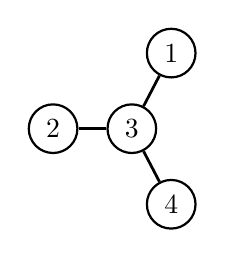
\begin{tikzpicture}[scale=1.0,auto,swap]

	  % define the round nodes
	  \foreach \pos/\name/\label in {
	    {(-2.0,1.46)/1/1a},
	    {(-3.5,0.5)/2/2a},
	    {(-2.5,0.5)/3/3a},
	    {(-2.0,-0.46)/4/4a}}
	    \node[vertex] (\label) at \pos {$\name$} ;

	  %neighbouring graph
		
	  \path[hi, line width=1.0]  (1a)  -- (3a);
	  \path[hi, line width=1.0]  (2a)  -- (3a);
	  \path[hi, line width=1.0]  (4a)  -- (3a);
    
	\end{tikzpicture}
	\caption{Claw}
	\label{fig:claw}
\end{subfigure}%
\begin{subfigure}{.2\textwidth}
	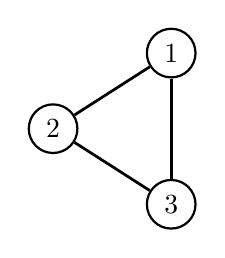
\begin{tikzpicture}[scale=1.0,auto,swap]

	  % define the round nodes
	  \foreach \pos/\name/\label in {
	    {(-2.0,1.46)/1/1a},
	    {(-3.5,0.5)/2/2a},
	    {(-2.0,-0.46)/3/3a}}
	    \node[vertex] (\label) at \pos {$\name$} ;

	  %neighbouring graph
		
	  \path[hi, line width=1.0]  (1a)  -- (2a);
	  \path[hi, line width=1.0]  (2a)  -- (3a);
	  \path[hi, line width=1.0]  (3a)  -- (1a);

	\end{tikzpicture}
	\caption{Cycle}
	\label{fig:cycle}
\end{subfigure}%
\begin{subfigure}{.2\textwidth}
	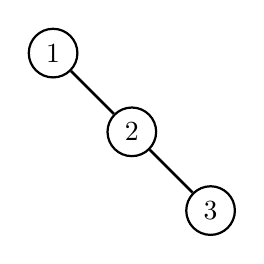
\begin{tikzpicture}[scale=1.0,auto,swap]

	  % define the round nodes
	  \foreach \pos/\name/\label in {
	    {(-3.0,1)/1/1a},
	    {(-2.0,0)/2/2a},
	    {(-1.0,-1)/3/3a}}
	    \node[vertex] (\label) at \pos {$\name$} ;

	  %neighbouring graph
		
	  \path[hi, line width=1.0]  (1a)  -- (2a);
	  \path[hi, line width=1.0]  (2a)  -- (3a);

	\end{tikzpicture}
	\caption{Path}
	\label{fig:path}
\end{subfigure}%
\begin{subfigure}{.2\textwidth}
	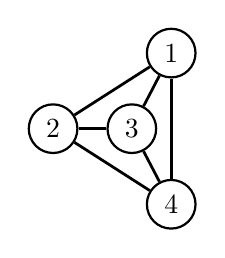
\begin{tikzpicture}[scale=1.0,auto,swap]

	  % define the round nodes
	  \foreach \pos/\name/\label in {
	    {(-2.0,1.46)/1/1a},
	    {(-3.5,0.5)/2/2a},
	    {(-2.5,0.5)/3/3a},
	    {(-2.0,-0.46)/4/4a}}
	    \node[vertex] (\label) at \pos {$\name$} ;

	  %neighbouring graph
		
	  \path[hi, line width=1.0]  (1a)  -- (2a);
	  \path[hi, line width=1.0]  (1a)  -- (3a);
	  \path[hi, line width=1.0]  (1a)  -- (4a);
	  \path[hi, line width=1.0]  (2a)  -- (3a);
	  \path[hi, line width=1.0]  (2a)  -- (4a);
	  \path[hi, line width=1.0]  (4a)  -- (3a);

	\end{tikzpicture}
	\caption{Clique}
	\label{fig:clique}
\end{subfigure}%
\end{center}
\caption[Graph types: claw, triangle, cycle and clique]{From left to right: A claw of 4 nodes ($C_4$), cycle of 3 nodes ($S_3$) (or triangle), a path of 3 nodes ($P_3$), a clique of 4 nodes ($K_4$).}
\label{graph_terminology_pic}
\end{figure}


\section{Global Network properties}

Global network properties give an overall picture of the network, but are unable to 
capture low-level patterns in the structure of the network. In the
following sections we will present a few key global properties such as the \emph{degree
distribution}, \emph{clustering coefficient} and the \emph{average path length}.

\subsection{Degree Distribution}

% \begin{figure}[h]
%   \centering
% 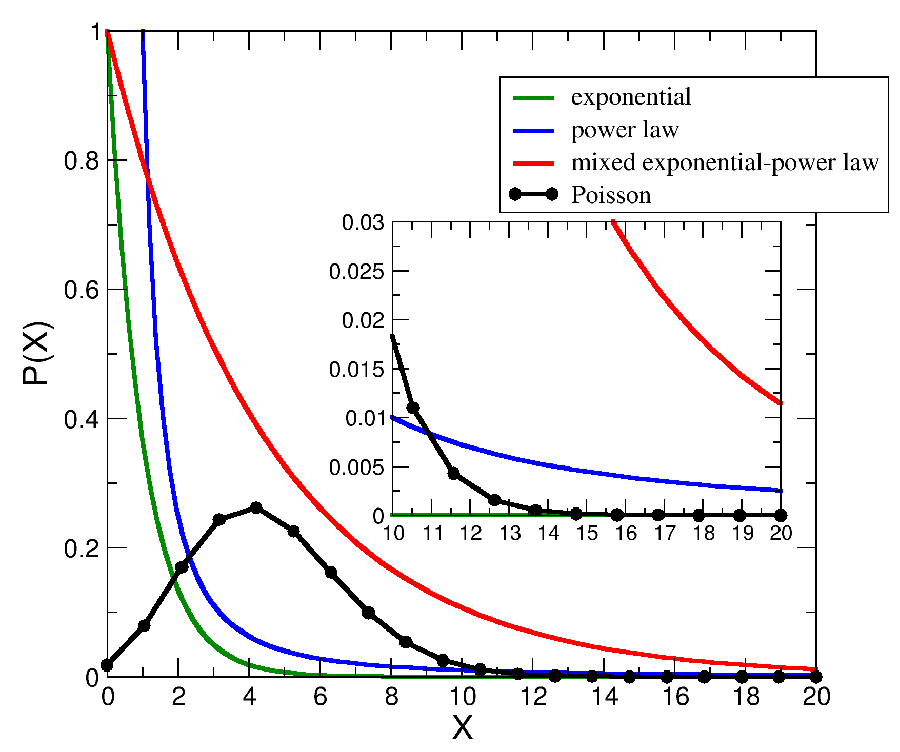
\includegraphics[scale=0.66]{images/deg_dist_all.png}
% \caption[Degree distributions: Poission, Power-law and Exponential.]{Some common classes of degree distributions:
% Poisson, Power-law and Exponential. Image source: \cite{dist2014proopnarine}}
% \label{fig:deg_dist_all}
% \end{figure}

\begin{mydef}
The degree of a node $x$ in a graph $G$ is the number of edges incident to the node, with loops counted twice. 
\end{mydef}

\begin{mydef}
The degree distribution $P(k)$ of a graph is the fraction of nodes in the network
having degree $k$. 
\end{mydef}

Several classes of degree distributions exist, with some most commonly-used ones being: 
\begin{itemize}
 \item Binomial
 \item Poison
 \item Power-law
 \item Exponential
\end{itemize}

% See figure \ref{fig:deg_dist_all} for an illustration of a Poison, Exponential and Power-law distributions. 

\begin{mydef}
A random variable $X$ follows the Bionomial distribution with parameters $n$ and $p$ if its probability mass function is given by:
$$ f(k;n,p) = {n \choose k} p^k (1-p)^{n-k}$$
\end{mydef}

\begin{mydef}
A random variable $X$ follows the Poisson distribution with parameter $\lambda > 0$ if its probability mass function is given by:
$$ f(k;\lambda) = \frac{\lambda^k e^{-\lambda}}{k!}$$
\end{mydef}

\begin{mydef}
A random variable $X$ follows the Power-law distribution with parameter $\gamma$ if its probability mass function is given by:
$$ f(k;\lambda) = k^{-\gamma}$$
\end{mydef}

A Power-law degree distribution has a high number of nodes with low degree and a very small number of nodes with high degree, also called hub nodes.

\begin{mydef}
A random variable $X$ follows the Exponential distribution with parameter $\lambda > 0$ if its probability mass function is given by:
$$ f(k;\lambda) = \lambda e^{-\lambda k}$$
\end{mydef}

Although many random graphs have a Poison degree distribution, it has been shown
that many real networks actually have a Power-law degree distribution instead. Such
networks include metabolic networks \cite{jeong2000large}, the Internet \cite{faloutsos1999power} and social networks \cite{adamic2001search}.

\subsection{Clustering Coefficient}

\begin{figure}[H]
\begin{center}
\begin{subfigure}{.3\textwidth}
  \centering
  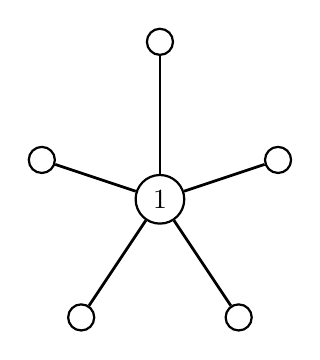
\begin{tikzpicture}[scale=1.0,auto,swap]

    % define the round nodes
    \foreach \pos/\name/\label in {
      {(-0.0,2.0)//2a},
      {(-1.5,0.5)//3a},
      {(-1.0,-1.5)//4a},
      {(1.0,-1.5)//5a},
      {(1.5,0.5)//6a}}
      \node[vertex2] (\label) at \pos {$\name$} ;
	      
    \foreach \pos/\name/\label in {
      {(-0.0,0.0)/1/1a}}
      \node[vertex] (\label) at \pos {$\name$} ;
      
    %neighbouring graph
	  
    \path[hi, line width=1.0]  (1a)  -- (2a);
    \path[hi, line width=1.0]  (1a)  -- (3a);
    \path[hi, line width=1.0]  (1a)  -- (4a);
    \path[hi, line width=1.0]  (1a)  -- (5a);
    \path[hi, line width=1.0]  (1a)  -- (6a);

  \end{tikzpicture}
  \caption{}
  \label{fig:clust1}
\end{subfigure}%
\begin{subfigure}{.3\textwidth}
  \centering
  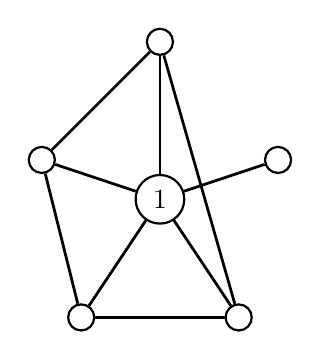
\begin{tikzpicture}[scale=1.0,auto,swap]

    % define the round nodes
    \foreach \pos/\name/\label in {
      {(-0.0,2.0)//2a},
      {(-1.5,0.5)//3a},
      {(-1.0,-1.5)//4a},
      {(1.0,-1.5)//5a},
      {(1.5,0.5)//6a}}
      \node[vertex2] (\label) at \pos {$\name$} ;
	      
    \foreach \pos/\name/\label in {
      {(-0.0,0.0)/1/1a}}
      \node[vertex] (\label) at \pos {$\name$} ;
      
    %neighbouring graph
	  
    \path[hi, line width=1.0]  (1a)  -- (2a);
    \path[hi, line width=1.0]  (1a)  -- (3a);
    \path[hi, line width=1.0]  (1a)  -- (4a);
    \path[hi, line width=1.0]  (1a)  -- (5a);
    \path[hi, line width=1.0]  (1a)  -- (6a);
    \path[hi, line width=1.0]  (2a)  -- (3a);
    \path[hi, line width=1.0]  (4a)  -- (5a);
    \path[hi, line width=1.0]  (4a)  -- (3a);
    \path[hi, line width=1.0]  (2a)  -- (5a);

  \end{tikzpicture}
  \caption{}
  \label{fig:clust2}
\end{subfigure}%
\begin{subfigure}{.3\textwidth}
  \centering
  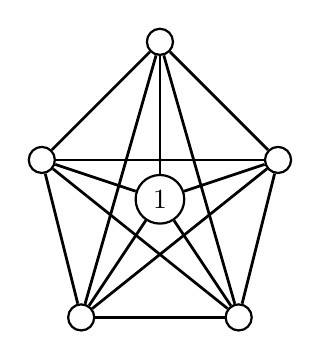
\begin{tikzpicture}[scale=1.0,auto,swap]

    % define the round nodes
    \foreach \pos/\name/\label in {
      {(-0.0,2.0)//2a},
      {(-1.5,0.5)//3a},
      {(-1.0,-1.5)//4a},
      {(1.0,-1.5)//5a},
      {(1.5,0.5)//6a}}
      \node[vertex2] (\label) at \pos {$\name$} ;
	      
    \foreach \pos/\name/\label in {
      {(-0.0,0.0)/1/1a}}
      \node[vertex] (\label) at \pos {$\name$} ;
      
    %neighbouring graph
	  
    \path[hi, line width=1.0]  (1a)  -- (2a);
    \path[hi, line width=1.0]  (1a)  -- (3a);
    \path[hi, line width=1.0]  (1a)  -- (4a);
    \path[hi, line width=1.0]  (1a)  -- (5a);
    \path[hi, line width=1.0]  (1a)  -- (6a);
    \path[hi, line width=1.0]  (2a)  -- (3a);
    \path[hi, line width=1.0]  (2a)  -- (4a);
    \path[hi, line width=1.0]  (2a)  -- (5a);
    \path[hi, line width=1.0]  (2a)  -- (6a);
    \path[hi, line width=1.0]  (3a)  -- (4a);
    \path[hi, line width=1.0]  (3a)  -- (5a);
    \path[hi, line width=1.0]  (3a)  -- (6a);
    \path[hi, line width=1.0]  (4a)  -- (5a);
    \path[hi, line width=1.0]  (4a)  -- (6a);
    \path[hi, line width=1.0]  (5a)  -- (6a);

  \end{tikzpicture}
  \caption{}
  \label{fig:clust3}
\end{subfigure}%
\end{center}
\caption[Clustering coefficient example]{The clustering coefficient intuitively describes how densely connected
the neighbours of a node are. In the above three scenarios, the
clustering coefficient $C$ of node 1 increases from $C = 0$ (image \subref{fig:clust1}) to 
$C = 1$ (image \subref{fig:clust3}) as more edges are added in its neighbourhood.}
\label{fig:clustering_coeff}
\end{figure}


The clustering coefficient is another important property of a graph that is used
for data analysis and comparisons. It measures the tendency of nodes to
cluster together, which is commonly seen in social networks.

Watts and Strogatz gave the following definition to the clustering coefficient \cite{watts1998collective}:
\begin{mydef}
 Let $G$ be a graph and $n$ a node that has $k_n $ neighbours. The maximum number of edges between the neighbours of $n$ is $
\frac{k_n (k_n - 1)}{2} $. The clustering coefficient of node $n$ is then defined 
as the fraction $ C_n $ of these edges that
are present in the set of neighbours of $n$. $ C_n $ can also be viewed as the
probability of two neighbours of $n$ being connected. This is then averaged
against all the nodes in the graph and the final clustering coefficient $C$ of
graph $G$ is obtained.  
\end{mydef}

It has been shown that real networks such as metabolic networks have a high clustering coefficient \cite{ravasz2002hierarchical}. Later on we will see that some random networks such as the Erd\H{o}s-R\'{e}nyi graphs have a low clustering coefficient when the
probability $p$ of connecting two nodes is also low. This makes these models unsuitable for modeling real data.

\subsection{Average path length}

\begin{mydef}
 Let $G =(V,E)$ be a graph and $u$ and $v$ two nodes in $V$. The distance between $u$ and $v$ is defined as the smallest number of links that have to be traversed to get from $u$ to $v$.
\end{mydef}

\begin{mydef}
 Let $G =(V,E)$ be a graph. The average path length of $G$ is the average distance between any pair of two nodes from $V$. 
\end{mydef}

Real networks have been shown to exhibit a small average path length. As a result, random network models that have been developed aimed at producing networks with a small average path length. Moreover, this property has several real-life applications. For example, in a real network such as the World Wide Web, a short average path length will facilitate the exchange of information and reduce operating costs. Similarly, a power grid will suffer less losses if its average path length is minimal.  \\


\subsection{Spectral Distribution}

Spectral network theory explains the topology of a network in terms of the eigenvalues and eigenvectors of matrices associated with the network, such as the adjacency matrix or Laplacian matrix. In order to understand the spectral distribution of a network we first need to define its Laplacian matrix.

\begin{mydef}
 Let $G = (V,E)$ be an unweighted graph and let $A$ be its adjacency matrix. The diagonal degree matrix $D$ of $G$ is a matrix where the diagonal entries are equal to the node degrees, that is $D(x,x) = d_x$, where $d_x$ is the degree of node $x$. The Laplacian matrix of $G$ is defined as:
 $$ L = D - A$$
\end{mydef}

\begin{mydef}
 Let $G$ be a graph and $L$ its Laplacian matrix. The spectral distribution of $G$ is defined as the ordered vector $\lambda = (\lambda_1, \lambda_2, \dots, \lambda_n)$ of eigenvalues of $L$ , where $\lambda_1$ is the largest eigenvalue and $\lambda_n$ the smallest.
\end{mydef}


The \emph{Spectral distance} between two graphs $G$ and $H$ is then defined as the Euclidean distance of their spectral distributions. Wilson and Zhou have analysed the spectral distribution of various networks and showed that the spectral distance of two networks is the best measure for classification and clustering purposes \cite{wilson2008study}. Thorne and Strumpf have also used the spectral distribution for the analysis of the evolution of PPI networks \cite{thorne2012graph}.

\section{Local Network properties}

Local network properties capture detailed information about a local region in the network or even about one single node of interest in the network. However, local properties cannot give an overall description of the network in the way the global properties such as the degree distribution or the average path length do. In the next few sections we will
present three main types of local network properties: \emph{Node centralities}, \emph{Graphlet
Frequency Vector} and \emph{Graphlet Degree Vector}

\subsection{Node centralities}

One commonly used property for measuring the importance of a node in a
network is the centrality. Several types of centralities exist:
\begin{itemize}
 \item \emph{Degree centrality}: Measures the number of links that connect with the
node. It is simply defined as the degree of the node.
 \item \emph{Betweenness centrality}: Quantifies how many shortest paths pass through
the node
 \item \emph{Closeness centrality}: Measures how close the node is to the other nodes
in the network.
\end{itemize}

\begin{mydef}
Let $G=(V,E)$ be a graph and $v$ a node from $V$. The Degree centrality of $v$ is defined as the degree of $v$.
\end{mydef}

\begin{mydef}
Let $G=(V,E)$ be a graph and $v$ a node from $V$. The Betweenness centrality of $v$ is defined as:
$$ B(v) = \sum_{s \ne v \ne t \in V}\frac{\sigma_{st}(v)}{\sigma_{st}}$$
where $\sigma_{st}(v) $ is the number of shortest paths from $s$ to $t$ that pass
through node $v$, while $ \sigma_{st} $ is the total number of shortest paths
from $s$ to $t$.
\end{mydef}


\begin{mydef}

Let $G=(V,E)$ be a graph, $v$ a node from $V$ and $d_v$ be the sum of the distances from $v$ to
all the other nodes in the network. The Closeness centrality $C_v$ is
defined as $C_v = d_v^{-1}$. 
\end{mydef}


\subsection{Graphlets}
\label{sec:graphlets}

\begin{figure}[h]
  \centering
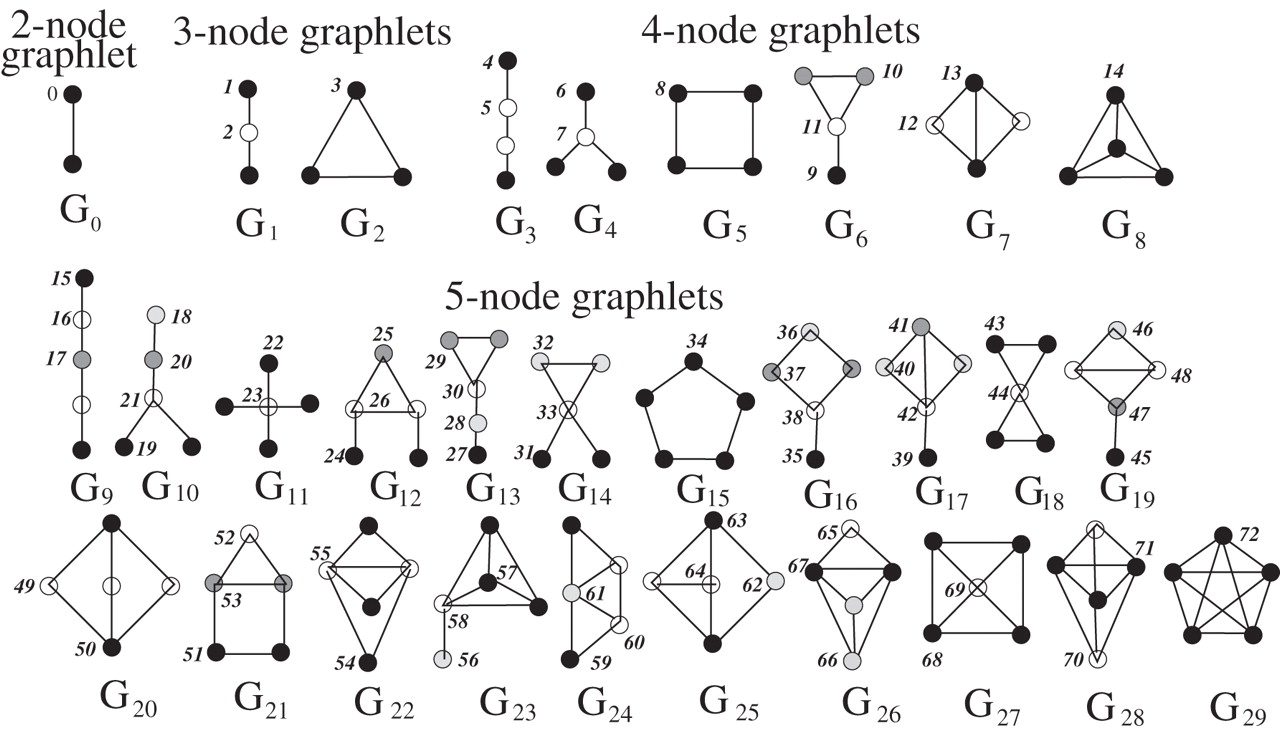
\includegraphics[scale=0.36]{images/graphlets.jpg}
\caption[Graphlets for sizes of 2, 3, 4 and 5 nodes]{Graphlets for sizes of 2, 3, 4 and 5 nodes. They are ordered in
groups according to the number of nodes they contain. These are the graphlets that are counted when computing
the GDV and GCV metrics. The node labels represent unique automorphism orbits. Source: \cite{milenkoviae2008uncovering} }
\label{fig:graphlets}
\end{figure}

Graphlets are small connected non-isomorphic\footnote{No two graphs from the set are the same.} induced\footnote{An induced subgraph is a subset of the vertices of a graph $G$ together with any edges whose endpoints are in the subset.} subgraphs of a graph. See definitions \ref{def:non_iso} and \ref{def:induced} for what non-isomorphic and induced graphs are. Figure \ref{fig:graphlets} shows all the graphlets of 2,3,4 and 5 nodes. They have been previously used by Nata\v{s}a et al. \cite{milenkoviae2008uncovering,prvzulj2007biological} for developing signatures such as the Graphlet Degree Vector (GDV) that quantify the local topological structure around a node.

For a given graph $G$, the \emph{Graphlet Frequency Vector} (GFV) can be calculated by
counting the number of distinct graphlets of each type found in $G$.
From here, we normalise the GFV against the total number of graphlets in $G$ to
calculate the \emph{Relative Graphlet Frequency Vector} (RGFV).

\begin{mydef}
\label{def:rgfv}
Let $G_i$ be the total number of graphlet of type $i$ in graph $G$. Then the Relative Graphlet Frequency Vector (RGFV) is defined as:

\begin{equation}
 GFV(G) = \left(F_1(G), F_2(G), ... F_{29}(G)\right)
\end{equation}
where 
$$ F_i(G) = -\log\left(\frac{G_i}{\sum_{i=1}^{n}G_i}\right) $$

\end{mydef}


\begin{figure}[h]
  \centering
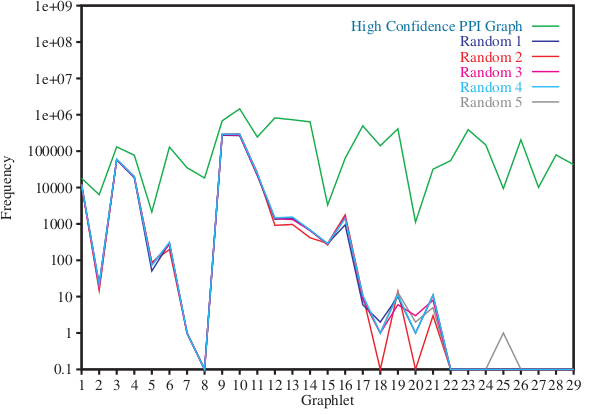
\includegraphics[scale=0.9]{images/gdv-er-interactome.png}
\caption[Graphlet Frequency Vectors for S. cerevisiae PPI network]{Example of \emph{Graphlet Frequency Vectors} for several random graphlets of a PPI network of
\emph{S. cerevisiae} (baker's yeast). As one can see from the plot, the GFV
signature of the real network is considerably different from the ones of the
random networks. The random networks have been generated using the Erd\H{o}s-R\'{e}nyi
method. Source: \cite{prvzulj2004modeling}}
\label{fig:gdv_er}
\end{figure}

\subsection{Relative Graphlet Frequency Distance}
\label{sec:rgfd}

Using the Graphlet frequencies that have been previously defined, we can now
compute a measure of disparity between two graphs by taking pairs of
graphlet frequencies for each type and then summing their absolute difference.
This is called the \emph{Relative Graphlet Frequency Distance} (RGFD). It is formally defined as follows:

\begin{mydef}
\label{def:rgfd}
Let $G$ and $H$ be two graphs and let \(F_i(G)\) and
\(F_i(H)\) be the frequency of the $i^{th}$ graphlet in $G$ and $H$ respectively. The Relative Graphlet Frequency Distance is then defined as:
$$  D = \sum_{i=1}^{n}| F_i(G) - F_i(H) | $$
\end{mydef}


\subsection{Graphlet Degree Vectors}
\label{sec:gdv}

In order to explain what a \emph{Graphlet Degree Vector} is, we first need to come back to automorphism orbits. For a node $x$, its automorphism orbit is the set of nodes similar to $x$ in the graph that could be interchanged with it in an automorphism operation. See definition \ref{def:automorphism_orbit} on page \pageref{def:automorphism_orbit} for a formal definition of the automorphism orbits. 


Figure \ref{fig:graphlets} shows the automorphism orbits for all the nodes in each of the 29 different graphlets. The different automorphism orbits are labelled with numbers ranging from 0 to 72, and the nodes in each graphlet are coloured according to which automorphism orbit it belongs to. Now that we have defined automorphism orbits, we can give a full definition of the \emph{Graphlet Degree Vector} of a node:

\begin{mydef}
For a node $x$ in a graph $G$, its Graphlet Degree Vector or GDV is a vector of $73$ coordinates, where each coordinate $i$ measures the number of graphlets that touch node $x$ at automorphism orbit $i$.
\end{mydef}

The GDV generalises the degree of a node, which counts the number of edges it touches, into the vector of graphlet degrees, which counts the number of graphlets that the node touches at a particular automorphism orbit. The resulting signature describes the local topology of the node neighbourhood up until a distance of 4 \cite{milenkoviae2008uncovering}.

For a given node $x$ in a graph $G$, we denote by $x_i$ the $i^{th}$ coordinate of the GDV vector of $x$. That is, $x_i$ is the number of times $x$ is touched at orbit $i$. 

\begin{mydef}
The distance $D_i(x,y)$ between the $i^{th}$ automorphism orbits of nodes $x$ and $y$ is defined as: 

\[D_i(x,y)=w_i \frac{|\log(x_i+1)-\log(y_i+1)|}{\log(\max(x_i,y_i)+2)}\]
where $w_i \in [0,1]$ are weights that normalise orbit dependency \emph{\cite{milenkoviae2008uncovering}}.
\end{mydef}

The logarithm function is used because the $i^{th}$ coordinates of the signature vectors of two nodes can differ by several order of magnitude and we do not want the distance measure to be dominated by the larger values \cite{milenkoviae2008uncovering}. We also add 1 to $u_i$ and $v_i$ in order to prevent the logarithm from going to $-\infty$. We add 2 in the denominator of the formula in order to prevent it from being infinite or 0 \cite{milenkoviae2008uncovering}.


\begin{mydef}
\label{def_gdv_dist}
Given two GDVs of nodes $x$ and $y$, the distance $D(x,y)$ between the GDVs of $x$ and $y$ is defined as:
$$D(x,y)= \frac{\sum_{i=0}^{72}D_i}{\sum_{i=0}^{72}w_i} $$ 
\end{mydef}

The distance measure given in definition \ref{def_gdv_dist} is in the $[0,1]$ range, where a distance of $0$ means that the two GDVs are identical. 

\begin{mydef}
\label{def_gdv_sim}
The signature similarity between nodes $x$ and $y$ is defined as:
$$S(x,y) = 1 - D(x,y) $$ 
\end{mydef}

The signature similarity gives a measure of how similar the topological structure around two nodes is. This is very useful because it can be easily applied to practical problems. For instance, it has been shown that the function of a protein can be predicted from its interactions \cite{letovsky2003predicting}. Therefore, if a protein $x$ is known to have a particular function and one would like to annotate a different, unknown protein $y$, one can transfer the function from $x$ to $y$ if their GDV signature similarity is high.

\subsection{Graphlet Degree Distributions}
\label{sec:gdd}

The Degree Distribution of a network calculates the number of nodes touching $k$
edges for each value of $k$. However, we can generalise this concept by looking
at the 73 automorphism orbits (see figure \ref{fig:graphlets}) and counting the
number of nodes that touch a particular graphlet at a particular orbit. Finally,
we get a spectrum of 73 \emph{Graphlet Degree Distributions (GDDs)} measuring
local properties of a network. 

We are now trying to compare the spectrum of 73 Graphlet Degree Distributions
belonging to a graph $G$ to the ones corresponding to another graph $H$. There
might be several ways to perform this, but we will present the method used by
N. Pr\v{z}ulj et al. in 2006 \cite{prvzulj2007biological}. 

\begin{mydef}

Let $G$ be a graph and let \( d_G^j(k) \) be a sample distribution of the
number of nodes in $G$ touching orbit $j$ ($j$ = $1-73$) $k$ times. \( d_G^j
\) represents the $j^{th}$ graphlet degree distribution (GDD). The scaled $j^{th}$ graphlet degree distribution $S_G^j(k)$ of $G$ is then defined as: 

$$ S_G^j(k) = \frac{d_G^j(k)}{k} $$

\end{mydef}


The reason for scaling \( d_G^j\) is because most of the information is retained in the lower
degrees, whereas the high degrees mostly contain
noise \cite{prvzulj2007biological}. Afterwards, the distribution is normalised
against its total area:

$$ T_G^j = \sum_{k=1}^{\infty}S_G^j(k) $$

giving the normalised distribution:

$$ N_G^j(k) = \frac{S_G^j(k)}{T_G^j}. $$

The reason why we are normalising the distribution is because a large
network would have a lot of nodes that potentially touch orbit $j$ and therefore a
large area under the curve. Normalising it would make large and small
biological networks comparable in terms of their GDD. 

\begin{mydef}
For two graphs $G$ and $H$ and an orbit $j$, we define the distance \( D^j(G,H) \) between their normalised $j^{th}$ distributions as:
$$ D^j(G,H) = \sqrt{\sum_{k=1}^{\infty}[N_G^j(k) - N_H^j(k)]^2} $$
\end{mydef}

The distance \( D^j(G,H) \) is between 0 and 1, where 0 means that $G$ and $H$ have
the same GDD for automorphism orbit $j$. Now that we have a measure of distance between two graphs $G$ and $H$, we need to invert the this distance in order to get the \emph{$j^{th}$ GDD agreement}:

\begin{mydef}

For two graphs $G$ and $H$ and an orbit $j$, we define the $j^{th}$ GDD agreement between their normalised $j^{th}$ distributions as:
$$ A^j(G, H) = 1 - D^j(G,H)$$
Moreover, the overall GDD agreement between the two
networks $G$ and $H$ is defined as the arithmetic mean of \( A^j(G,H) \) over all $j$:
 
$$ A(G,H) = \frac{1}{73}\sum_{j=0}^{72}A^j(G,H) $$  
\end{mydef}

The GDD agreement is like the GDV signature similarity of two nodes $x$ and $y$, but this time for the overall graphs $G$ and $H$. This measure can be used to compare different networks or even evaluate which random graphs best model the real data.

\section{Random graphs}

Random graphs are graphs that are usually generated using a random process. They are used in data analysis for comparing or aligning them against real networks. They can model the behaviour of real-world networks, such as the World Wide Web or PPI networks. Random graph models have been successfully used in various biological settings, such as: Network motifs \cite{milo2002network}, De-noising of protein-protein interaction network data \cite{kuchaiev2009geometric} or guiding biological experiments \cite{lappe2003unraveling}. In the next sections we will present several types of random graphs along with their properties.

\subsection{Erd\H{o}s-R\'{e}nyi graphs}

The work on random graph models started from the influential publications of
Erd\H{o}s and R\'{e}nyi in the 1950s and 1960s. Edgar Gilbert also published a similar
model later on. Erd\H{o}s and R\'{e}nyi described the \(G_{n,m}\)
model \cite{erdHos1959random}, while Gilbert described the \(G_{n,p}\)
model \cite{gilbert1959random}. These two methods can be described as
follows: 
\begin{itemize}
 \item[\(\mathbf{G_{n,p}}\)]: We start with $n$ disconnected nodes and a given
probability $p$. We then go through every pair of nodes and connect them with
probability $p$.
 \item[\(\mathbf{G_{n,m}}\)]: We start with $n$ disconnected nodes and a target number of edges $m$. Afterwards, we randomly select $m$ pairs of nodes and connect them.
\end{itemize}

Although these networks are very easy to generate, it was later found
that real networks have a structure that is different from the
Erd\H{o}s-R\'{e}nyi graphs. More precisely, they have a different degree distribution and a low clustering coefficient. On the other hand, some real networks have a power-law degree distribution. For the Erd\H{o}s-R\'{e}nyi $ G_{n,p} $ graph, the degree distribution is binomial:

\begin{equation}
 P(k) = {n-1 \choose k} p^k (1-p)^{n-1-k}
\end{equation}
which can be approximated with a Poisson distribution for a large $n$:

\begin{equation}
 P(k) = \frac{z^k * e^{-z}}{k!}
\end{equation}

\begin{figure}[H]
\begin{center}
\begin{subfigure}{.3\textwidth}
  \centering
  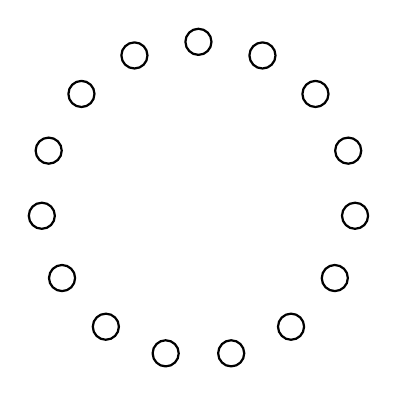
\begin{tikzpicture}[scale=1.0,auto,swap]

    % define the round nodes
    \foreach \pos/\name/\label in {
	{(0.000, 2.000)//0a},
	{(0.813, 1.827)//1a},
	{(1.486, 1.338)//2a},
	{(1.902, 0.618)//3a},
	{(1.989, -0.209)//4a},
	{(1.732, -1.000)//5a},
	{(1.176, -1.618)//6a},
	{(0.416, -1.956)//7a},
	{(-0.416, -1.956)//8a},
	{(-1.176, -1.618)//9a},
	{(-1.732, -1.000)//10a},
	{(-1.989, -0.209)//11a},
	{(-1.902, 0.618)//12a},
	{(-1.486, 1.338)//13a},
	{(-0.813, 1.827)//14a}}
      \node[vertex2] (\label) at \pos {$\name$} ;
	  


  \end{tikzpicture}
  \caption{$p = 0$}
  \label{fig:p00}
\end{subfigure}%
\begin{subfigure}{.3\textwidth}
  \centering
  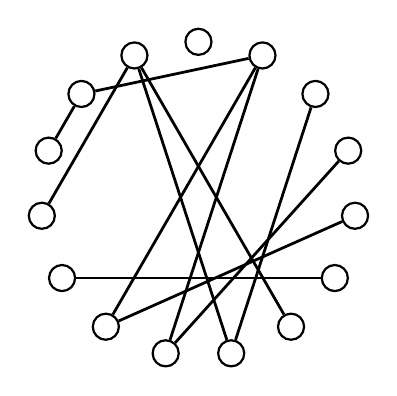
\begin{tikzpicture}[scale=1.0,auto,swap]

    % define the round nodes
    \foreach \pos/\name/\label in {
	{(0.000, 2.000)//0a},
	{(0.813, 1.827)//1a},
	{(1.486, 1.338)//2a},
	{(1.902, 0.618)//3a},
	{(1.989, -0.209)//4a},
	{(1.732, -1.000)//5a},
	{(1.176, -1.618)//6a},
	{(0.416, -1.956)//7a},
	{(-0.416, -1.956)//8a},
	{(-1.176, -1.618)//9a},
	{(-1.732, -1.000)//10a},
	{(-1.989, -0.209)//11a},
	{(-1.902, 0.618)//12a},
	{(-1.486, 1.338)//13a},
	{(-0.813, 1.827)//14a}}
      \node[vertex2] (\label) at \pos {$\name$} ;
	      
    %neighbouring graph
	  
    \path[hi, line width=1.0]  (7a)  -- (2a);
    \path[hi, line width=1.0]  (8a)  -- (1a);
    \path[hi, line width=1.0]  (8a)  -- (3a);
    \path[hi, line width=1.0]  (9a)  -- (1a);
    \path[hi, line width=1.0]  (9a)  -- (4a);
    \path[hi, line width=1.0]  (10a)  -- (5a);
    \path[hi, line width=1.0]  (13a)  -- (1a);
    \path[hi, line width=1.0]  (13a)  -- (12a);
    \path[hi, line width=1.0]  (14a)  -- (6a);
    \path[hi, line width=1.0]  (14a)  -- (7a);
    \path[hi, line width=1.0]  (14a)  -- (11a);


  \end{tikzpicture}
  \caption{$p = 0.1$}
  \label{fig:p01}
\end{subfigure}%
\begin{subfigure}{.3\textwidth}
  \centering
  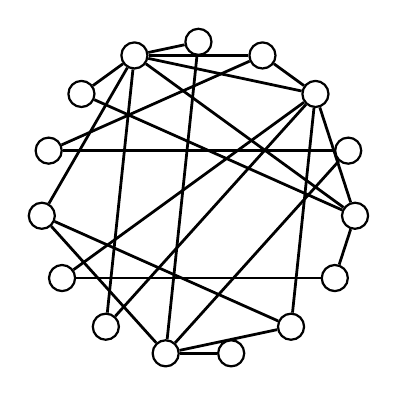
\begin{tikzpicture}[scale=1.0,auto,swap]

    % define the round nodes
    \foreach \pos/\name/\label in {
	{(0.000, 2.000)//0a},
	{(0.813, 1.827)//1a},
	{(1.486, 1.338)//2a},
	{(1.902, 0.618)//3a},
	{(1.989, -0.209)//4a},
	{(1.732, -1.000)//5a},
	{(1.176, -1.618)//6a},
	{(0.416, -1.956)//7a},
	{(-0.416, -1.956)//8a},
	{(-1.176, -1.618)//9a},
	{(-1.732, -1.000)//10a},
	{(-1.989, -0.209)//11a},
	{(-1.902, 0.618)//12a},
	{(-1.486, 1.338)//13a},
	{(-0.813, 1.827)//14a}}
      \node[vertex2] (\label) at \pos {$\name$} ;
	      
    %neighbouring graph
	  
    \path[hi, line width=1.0]  (2a)  -- (1a);
    \path[hi, line width=1.0]  (4a)  -- (2a);
    \path[hi, line width=1.0]  (5a)  -- (4a);
    \path[hi, line width=1.0]  (6a)  -- (2a);
    \path[hi, line width=1.0]  (8a)  -- (0a);
    \path[hi, line width=1.0]  (8a)  -- (3a);
    \path[hi, line width=1.0]  (8a)  -- (6a);
    \path[hi, line width=1.0]  (8a)  -- (7a);
    \path[hi, line width=1.0]  (9a)  -- (2a);
    \path[hi, line width=1.0]  (10a)  -- (2a);
    \path[hi, line width=1.0]  (10a)  -- (5a);
    \path[hi, line width=1.0]  (11a)  -- (6a);
    \path[hi, line width=1.0]  (11a)  -- (8a);
    \path[hi, line width=1.0]  (12a)  -- (1a);
    \path[hi, line width=1.0]  (12a)  -- (3a);
    \path[hi, line width=1.0]  (13a)  -- (4a);
    \path[hi, line width=1.0]  (14a)  -- (0a);
    \path[hi, line width=1.0]  (14a)  -- (1a);
    \path[hi, line width=1.0]  (14a)  -- (2a);
    \path[hi, line width=1.0]  (14a)  -- (4a);
    \path[hi, line width=1.0]  (14a)  -- (9a);
    \path[hi, line width=1.0]  (14a)  -- (11a);
    \path[hi, line width=1.0]  (14a)  -- (13a);



  \end{tikzpicture}
  \caption{$p = 0.2$}
  \label{fig:p02}
\end{subfigure}%
\end{center}
\caption[Erd\H{o}s-R\'{e}nyi graphs]{Example of three Erd\H{o}s-R\'{e}nyi random graphs generated using the
\(G_{n,p}\) method. The three different graphs differ with respect to the
probability $p$ of connecting one pair of nodes: (\subref{fig:p00}) $p = 0$ -- the graph is completely
disconnected. (\subref{fig:p01}) $p = 0.1$ -- the graph is sparsely connected because the probability $p$ is low
(\subref{fig:p02}) $p = 0.2$ -- the graph becomes more dense because of the increase of $p$ .}
\label{fig:erdos_renyi_graphs}
\end{figure}


\subsection{Erd\H{o}s-R\'{e}nyi with preserved degree distribution}
\label{er-dd}

As we have previously seen, the degree distribution of an Erd\H{o}s-R\'{e}nyi graph
does not match the real data. We will now present a method for constructing an
Erd\H{o}s-R\'{e}nyi network that preserves the degree distribution of a real network. 

We start with $n$ disconnected nodes. Each node is assigned a number of stubs 
according to the degree distribution of the real network that is being
modelled. A stub is simply a slot belonging to a particular node from where an edge can 
be connected. Afterwards, edges are created only between random pairs of nodes with
available stubs. After an edge is created, the number of stubs left available
at the nodes that were just connected is decreased by one. Moreover, edges
between one node and itself are not allowed.

This "stubs method" allows us to create Erd\H{o}s-R\'{e}nyi networks that have a power-law
degree distribution and a small average path length. Unfortunately, they still
have a low clustering coefficient.

\subsection{Scale-free networks}

\begin{figure}
  \centering
  \begin{subfigure}[b]{0.4\textwidth}
    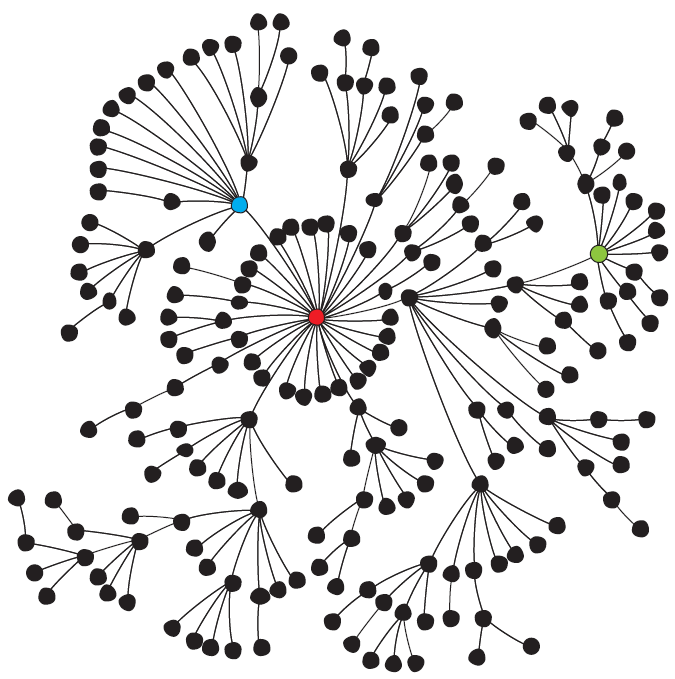
\includegraphics[width=\textwidth]{images/scale-free-network.png}
    \caption[Scale free network]{Example of a scale-free network. Note the large
    number of nodes of small degree at the periphery of the network, while the
    number of hub nodes is very small.}
    \label{fig:scale_free_network}  
  \end{subfigure}
  ~ %add desired spacing between images, e. g. ~, \quad, \qquad etc.
    %(or a blank line to force the subfigure onto a new line)
  \begin{subfigure}[b]{0.5\textwidth}
    \centering
    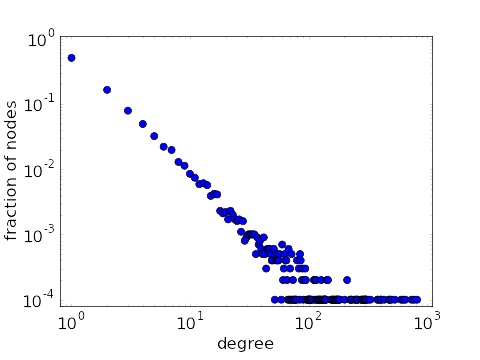
\includegraphics[width=\textwidth]{images/deg_dist_scale_free.png}
    \caption{The power-law degree distribution of a scale-free network. As the degree of
the nodes gets larger, the fraction of nodes decreases exponentially. Notice
the logarithmic scale on the Y axis. It has been observed that many real
networks exhibit a power-law degree distribution \cite{jeong2000large,faloutsos1999power,adamic2001search}.}
    \label{fig:degree_distribution}    
   \end{subfigure}
   \caption[Power-law degree distribution of a scale free network]{Scale-free network (\subref{fig:scale_free_network}) and power-law degree distribution (\subref{fig:degree_distribution})}
   \label{fig:scale_free} 
\end{figure}


Scale-free networks are networks that normally exhibit a power-law degree
distribution (see fig \ref{fig:scale_free}). That is, $ P(k) = k^{-\gamma} $,
where $P(k)$ is the fraction of nodes having degree $k$. It is currently believed that many networks such as the
World Wide Web, social networks or biological networks exhibit scale-free properties with a power-law degree distribution.

\subsubsection{Barab\'{a}si-Albert model}

There are several proposed ways in which scale-free networks can be
generated. The Barab\'{a}si-Albert model is one such technique that uses the
\emph{preferential attachment} mechanism, with which nodes of high degree have
a high probability of receiving even more connections. 

In order to construct a network using the Barab\'{a}si-Albert method, we start with
an initial connected network of $ m_0  $ nodes. New nodes are consecutively
added to the network one at a time. Each one of them is connected to $ m \le m_0 
$ target nodes with a probability that is proportional to the degree of the
target nodes. Formally, the probability $ p_i $ that the new node is connected
to node $i$ is:

\begin{equation}
 p_i = \frac{k_i}{\sum_{j}k_j}
\end{equation}

where $ k_i $ is the degree of node $i$, while the sum is over all the
nodes $j$ that already existed in the network when the new node is added. Because
of the preferential mechanism, heavily linked nodes (also called hub nodes)
tend to quickly accumulate links, whereas nodes with a low degree are unlikely
to be chosen. It has also been shown that the starting network heavily
influences the properties of the resulting network \cite{hormozdiari2007not}.

\subsection{Geometric graphs}

Geometric graphs are generated by fixing a certain metric space and using
metrics such as geometric distance or radius to connect edges together. A
metric space is a space that has a distance norm associated to it such as: the
Euclidean distance, Chessboard distance or Manhattan distance.

Such a network is generated in the following manner:
\begin{enumerate}
 \item Choose a metric space and place nodes within the space using a uniform
random distribution.
 \item If any nodes are within distance $d$ from each other, then connect them
with an edge.
 \item $d$ needs to be chosen so that the end number of edges matches the network
that is modelled.
\end{enumerate}

\begin{figure}[H]
  \centering
  \begin{subfigure}[b]{0.45\textwidth}
    \centering
    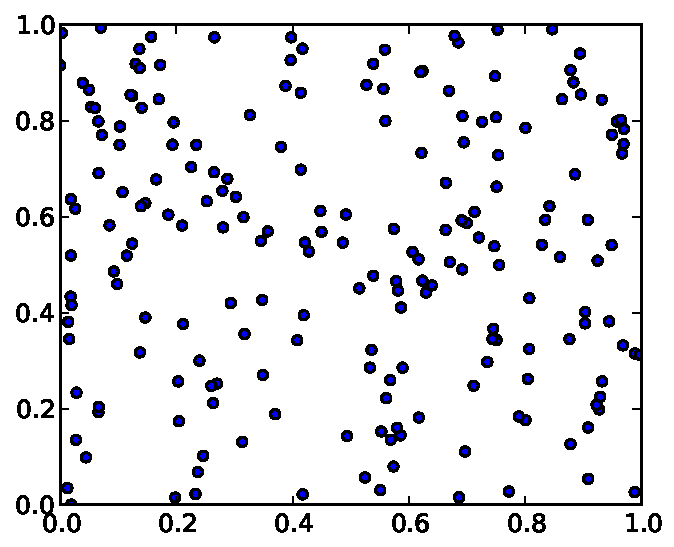
\includegraphics[scale=0.65]{../code/final_results/geometric_graphs/geo1.pdf}
    \caption{$d = 0.0$}
    \label{fig:geo1}  
  \end{subfigure}
  ~ %add desired spacing between images, e. g. ~, \quad, \qquad etc.
    %(or a blank line to force the subfigure onto a new line)
  \begin{subfigure}[b]{0.45\textwidth}
    \centering
    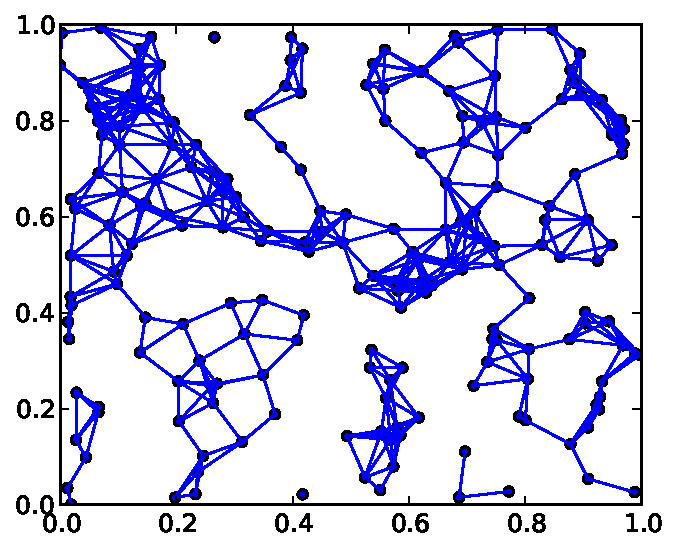
\includegraphics[scale=0.65]{../code/final_results/geometric_graphs/geo2.pdf}
    \caption{$d = 0.1$}
    \label{fig:geo2}    
   \end{subfigure}
    ~ %add desired spacing between images, e. g. ~, \quad, \qquad etc.
    %(or a blank line to force the subfigure onto a new line)
  \begin{subfigure}[b]{0.45\textwidth}
    \centering
    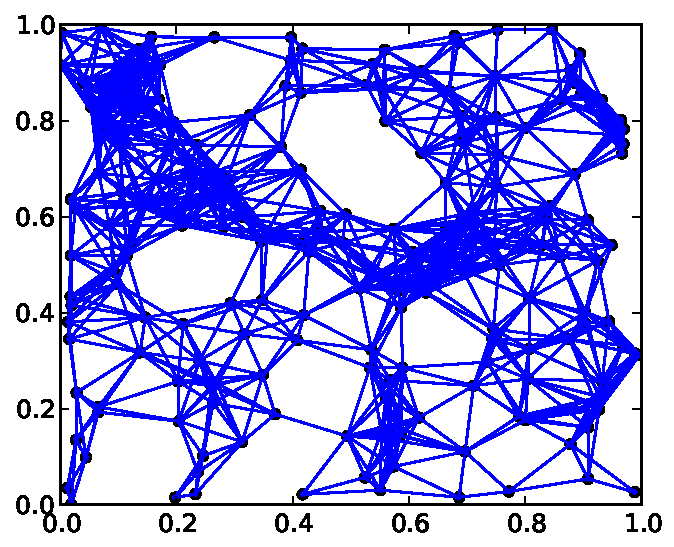
\includegraphics[scale=0.65]{../code/final_results/geometric_graphs/geo3.pdf}
    \caption{$d = 0.15$}
    \label{fig:geo3}    
   \end{subfigure}
    ~ %add desired spacing between images, e. g. ~, \quad, \qquad etc.
    %(or a blank line to force the subfigure onto a new line)
  \begin{subfigure}[b]{0.45\textwidth}
    \centering
    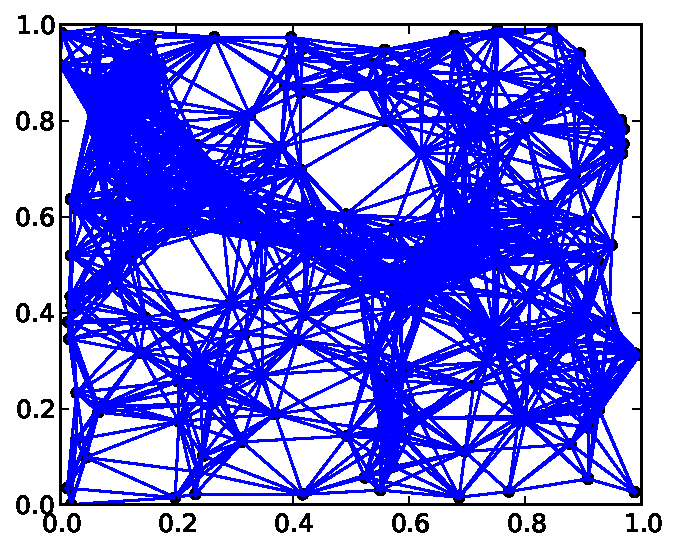
\includegraphics[scale=0.65]{../code/final_results/geometric_graphs/geo4.pdf}
    \caption{$d = 0.2$}
    \label{fig:geo4}    
   \end{subfigure}
   \caption[Geometric random graphs]{Geometric random networks built using different values for the distance parameter $d$, starting from
$d = 0$. Initially, nodes are distributed randomly across a metric space. When $d = 0$ in graph (\subref{fig:geo1}), the nodes are all disconnected from each other. As $d$ increases in graphs (\subref{fig:geo2} -- \subref{fig:geo4}), the number of connections in the network also increases proportionally. When using a Geometric network to model a real network, one would normally use a value of $d$ that would yield a similar number of edges as the real network.}
   \label{fig:geometric} 
\end{figure}


\subsection{Stickiness index-based graphs}

Pr\v{z}ulj et al. have proposed in 2006 a simple random
graph model that inserts a connection according to the degree or \emph{stickiness}
of the nodes involved \cite{prvzulj2006modelling}. This model has been inspired
from analysing protein-protein interactions and is based on two assumptions:
\begin{enumerate}
 \item A node with a high degree or \emph{stickiness} represents a protein that has many binding domains and/or its binding domains are
commonly involved in interactions.
 \item A pair of proteins is more likely to interact, or share complementary
binding domains, if they both have a high \emph{stickiness}. On the other hand,
if one or both of them have a low \emph{stickiness} index, they are less likely to
interact. Thus, the product of their stickiness values can be used as the
probability of connecting the nodes.
\end{enumerate}

Considering the above assumptions, a stickiness based random graph can be
constructed as follows:
\begin{enumerate}
 \item We start with a network of $n$ nodes each having a degree $ deg_i $
sampled from a degree distribution of our choice
 \item For each node $i$, we compute the stickiness index $
\theta_i=deg_i/\sqrt{\sum_{j=1}^{N}deg_j}. $ Note that $ 0 \leq \theta_i \leq 1$
 \item For each pair of nodes $(i,j)$, we connect them with probability $
\theta_i \theta_j $
\end{enumerate}


\subsection{Random graph Comparisons}

Now that we have presented a few commonly used random graph generating methods, we would like to compare them in terms of their underlying properties. As can be clearly seen in table \ref{tab:network_comparison}, real networks
normally have a power-law degree distribution, high clustering coefficient and
a small average path length. In terms of degree distribution, only Erd\H{o}s-R\'{e}nyi
(with a preserved degree distribution), Barab\'{a}si-Albert and Stickiness-based
random networks have a power-law degree distribution, which is found in real
networks. However, it must be noted that although most of the real networks
have a power-law degree distribution, this subject is still a matter of research. For
example, it has been shown that the Interactome network can be better modelled with
a Geometric network that has a Poisson degree distribution \cite{prvzulj2004modeling}.

On the other hand, only the Geometric and the Stickiness based models have a
high clustering coefficient. This is again something which has been observed in
most of the real networks such as social networks or biological networks.
Finally, most of the networks have a small average path length. It can
therefore be noted that the Stickiness-based network is the most successful
at modeling real-world phenomena with respect to these three properties.
However, there might be other network properties, such as various node
centralities \cite{newman2009networks} or \emph{Relative Graphlet Frequency
Agreement}, with can also be employed to
assess the suitability of the random networks. Identifying which of these 
properties can best compare various types of networks is still an open problem in
Network Analysis.

\definecolor{blue3}{HTML}{86B7FC} % med blue
\definecolor{blue1}{HTML}{B5F1FF} % light blue
\definecolor{blue2}{HTML}{E0F9FF} % very light blue

\definecolor{darkgreen}{HTML}{000000} % dark green

\rowcolors{1}{blue1}{blue2}

\begin{table}
  \centering
  Comparison of real networks versus randomly generated networks 
  \begin{tabular}{ | l | c | c | c |  }
%     \hlinede
    \cellcolor{blue3} Model & \cellcolor{blue3} Degree Distribution &
  \cellcolor{blue3} Clustering coefficient & \cellcolor{blue3} Average path
length \\
    \hline
    Real networks & \textcolor{darkgreen}{Power-law} &
  \textcolor{darkgreen}{High} & \textcolor{darkgreen}{Small}\\
    \hline
    Erd\H{o}s-R\'{e}nyi & \textcolor{red}{Poisson} & \textcolor{red}{Low} &
  \textcolor{red}{Large (for small p)} \\
    \hline
    Erd\H{o}s-R\'{e}nyi - DD & \textcolor{darkgreen}{Power-law} &
  \textcolor{red}{Low} & \textcolor{darkgreen}{Small} \\
    \hline
    Barab\'{a}si-Albert & \textcolor{darkgreen}{Power-law} &
  \textcolor{red}{Low} & \textcolor{darkgreen}{Small} \\
    \hline
    Geometric (uniform) & \textcolor{red}{Poisson} &
  \textcolor{darkgreen}{High} & \textcolor{darkgreen}{Small} \\
    \hline
    Stickiness based & \textcolor{darkgreen}{Power-law} &
  \textcolor{darkgreen}{High} & \textcolor{darkgreen}{Small} \\
    \hline
  \end{tabular}
  \caption{As one can observe from the table above, some of the models
such as Erd\H{o}s-R\'{e}nyi are not suitable for modeling real networks according to
these metrics. On the other hand, the Stickiness based random graph satisfies all the three criteria. Nevertheless, other network properties might exist for which the Stickiness based random network does not match the corresponding real network.}
  \label{tab:network_comparison}
\end{table}

\section{Measuring Correlation}

In sections \ref{sec:rgfd} and \ref{sec:gdd} we presented two main methods for calculating
how closely two GDV vectors match: \emph{Relative Graphlet Frequency Distance}
 and \emph{Graphlet Degree Distribution Agreement}. However, other methods also exist that use correlation coefficients such as \emph{Pearson's product-movement correlation coefficient} or \emph{Spearman's rank correlation coefficient}. This section presents correlation techniques that can be used for GDV comparisons.

\subsection{Pearson's product-movement correlation coefficient}

Given two random variables $X$ and $Y$ from a population, \emph{Pearson's
correlation coefficient} or sometimes called \emph{Pearson's population
correlation coefficient} is defined as the ratio between the covariance of $X$
and $Y$ and the product of their standard deviation. It was introduced by Karl
Pearson and it is based on a similar idea by Francis Galton in 1880 \cite{stigler1989francis,lee1988thirteen}.

\begin{mydef}
The Pearson's product-movement correlation coefficient $ \rho_{X,Y} $ between random variables $X$ and $Y$ is defined as:

 $$ \rho_{X,Y} = \frac{\sigma_{XY}}{\sigma_X\sigma_Y} =
\frac{E[X-\mu_X]E[Y-\mu_Y]}{\sigma_X\sigma_Y}$$
where $ \sigma_{XY} $ is the covariance of $X$ and $Y$, while $\sigma_X $, $ \mu_X $ and $\sigma_Y $, $ \mu_Y $ are the standard deviation and the expectation of $X$ and $Y$ respectively.
\end{mydef}


Pearson's correlation coefficient can also be applied to a sample from a given
population, in which case it is called the \emph{sample Pearson's correlation
coefficient} and is commonly denoted by $r$. This can be calculated by using
sample estimators for the covariance and standard deviation in the formula
above. 

\begin{mydef}
The sample Pearson's product-movement correlation coefficient $ r_{X,Y} $ between population samples $X$ and $Y$ is defined as:

\begin{equation}
\label{pears_corr}
 r = \frac{\sum_{i=1}^{n}(X_i - \bar{X})(Y_i -
\bar{Y})}{\sqrt{\sum_{i=1}^{n}\left(X_i -
\bar{X}\right)^2}\sqrt{\sum_{i=1}^{n}\left(Y_i -
\bar{Y}\right)^2}} 
\end{equation}
where $ \sigma_{XY} $ is the covariance of $X$ and $Y$, while $\sigma_X $, $ \mu_X $ and $\sigma_Y $, $ \mu_Y $ are the standard deviation and the expectation of $X$ and $Y$ respectively.
\end{mydef}

The values of both the sample and the population variants of Pearson's
correlation coefficients are between -1 and 1. Sample data points that have 
exactly 1 or -1 as their correlation coefficient will lie on a straight line.
Moreover, Pearson's correlation coefficient is symmetric because: 

$$ \rho(X,Y) = \rho(Y,X) $$

where $\rho(X,Y)$ is defined as the correlation between random variables $X$ and $Y$.

\subsubsection{Pearson's distance}

Given a correlation coefficient $ \rho_{X,Y} $, a distance metric
called the \emph{Pearson's distance} can be derived as
follows \cite{fulekar2009bioinformatics}:

$$ d_{X,Y} = 1- \rho_{X,Y} $$

It should be noted that because Pearson's correlation coefficient lies between
-1 and 1, then the Pearson's distance will have a value between 0 and 2.

\subsubsection{Interpretation}

Several researchers have provided guidelines into how
to interpret the size of the correlation coefficient \cite{cohen1988statistical} 
(equation \ref{pears_corr}). However, interpretation is highly dependent on the context of the problem. For
example, a correlation of 0.8 might be low if one verifies physical laws using
measurements made with high-precision instruments, but it might be considered
high when applied to the analysis of social networks, because of underlying hidden
factors.

\subsection{Spearman's rank correlation coefficient}


% perf: pears (0.914, 0.000) spear (1.000, 0.000)
% spread: pears (0.086, 0.447) spear (0.114, 0.314)
% outliers: pears (0.557, 0.000) spear (0.810, 0.000)

\rowcolors{1}{}{}


\begin{figure}[h]
\begin{center}	
\begin{subfigure}{0.45\textwidth}
  \centering
  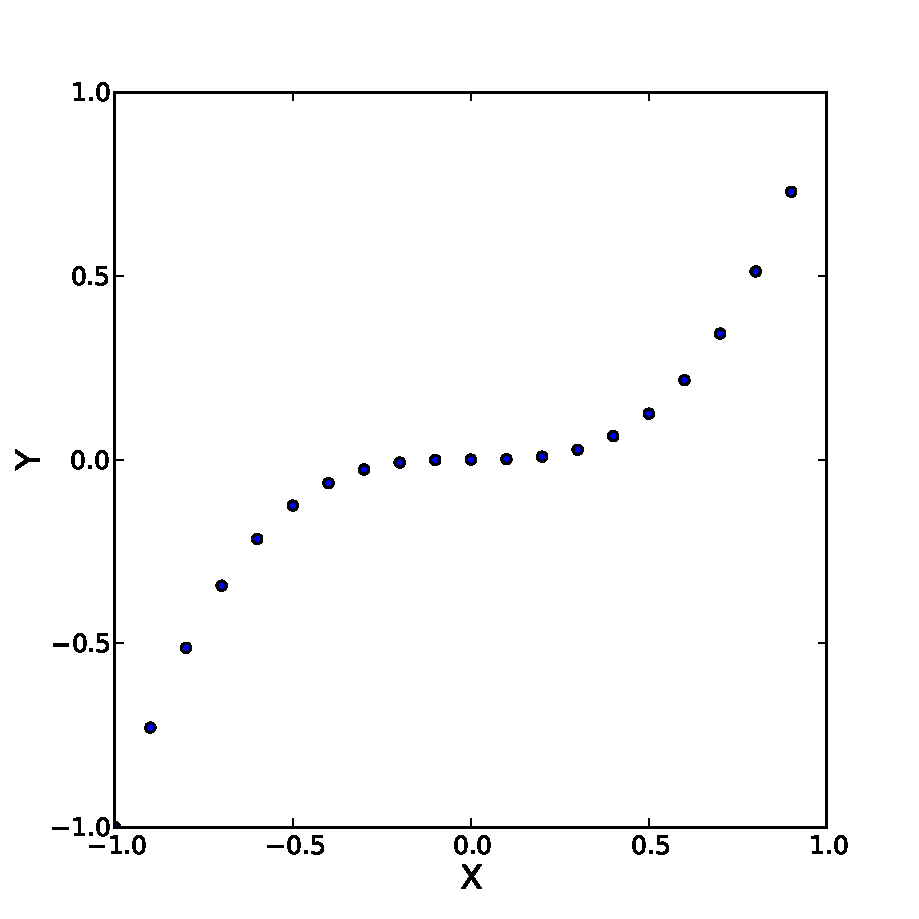
\includegraphics[width=\columnwidth]{../code/final_results/spearman_images/perfect.pdf}
  \caption{\begin{tabular}{r l}
 Pearson correlation: & 0.91\\
 p-value: & 0.0\\
 \hline
 Spearman correlation: & 1.0\\
 p-value: & 0.0
\end{tabular}}
  \label{fig:perf}
\end{subfigure}
\begin{subfigure}{0.45\textwidth}
  \centering
  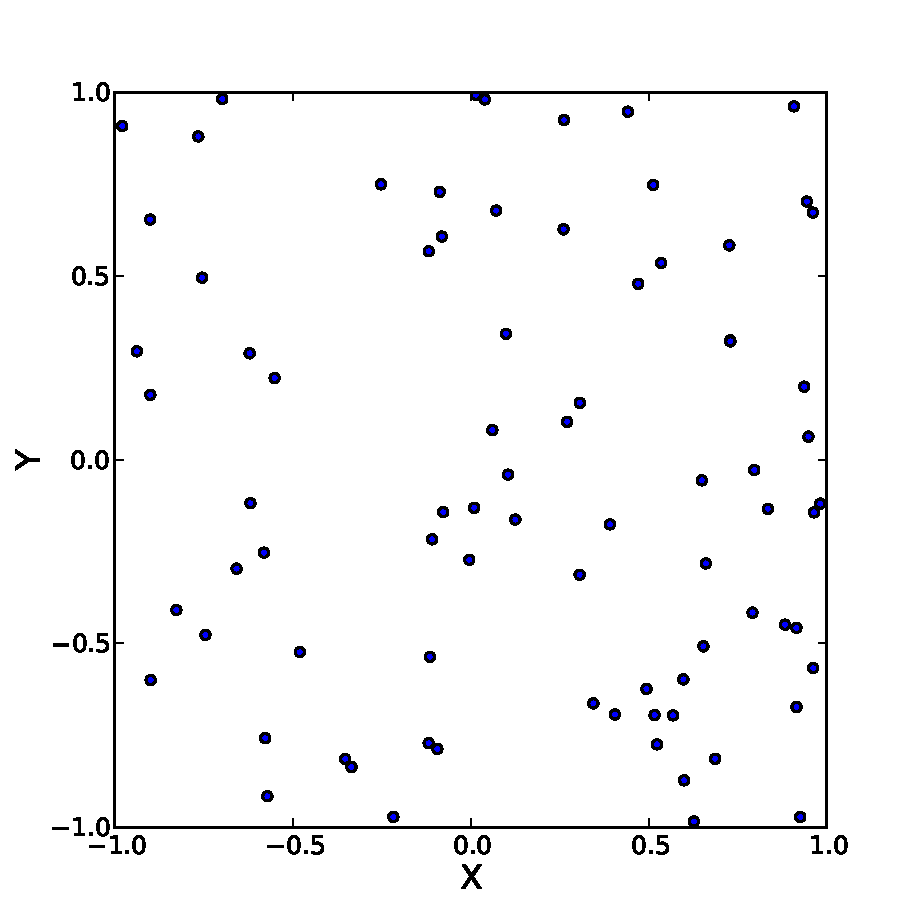
\includegraphics[width=\columnwidth]{../code/final_results/spearman_images/spread.pdf}
  \caption{\begin{tabular}{r l}
 Pearson correlation: & 0.08\\
 p-value: & 0.44\\
 \hline
 Spearman correlation: & 0.11\\
 p-value: & 0.31
\end{tabular}}  \label{fig:spread}
\end{subfigure}
\end{center}
\caption[Spearman's correlation coefficient -- perfectly correlated data vs random data ]{Spearman's correlation coefficient is measuring how well the
dependence between two variables $X$ and $Y$ can be modelled
using a monotonic function. A Spearman's correlation of 1 can result even
when the data points are not linear (subfigure \subref{fig:perf}), as long as they are monotonically related. For the same dataset, Pearson's correlation coefficient is 0.91. When the data points are evenly spread (subfigure \subref{fig:spread}), both the Pearson's and the Spearman's
correlation coefficients will be low ( 0.08 and
0.11 respectively) and their p-value will be high (0.44 and 0.31), suggesting that the correlation is not statistically significant.}
\end{figure}


\begin{figure}[h]
\begin{center}
\begin{subfigure}{0.45\textwidth}
  \centering
  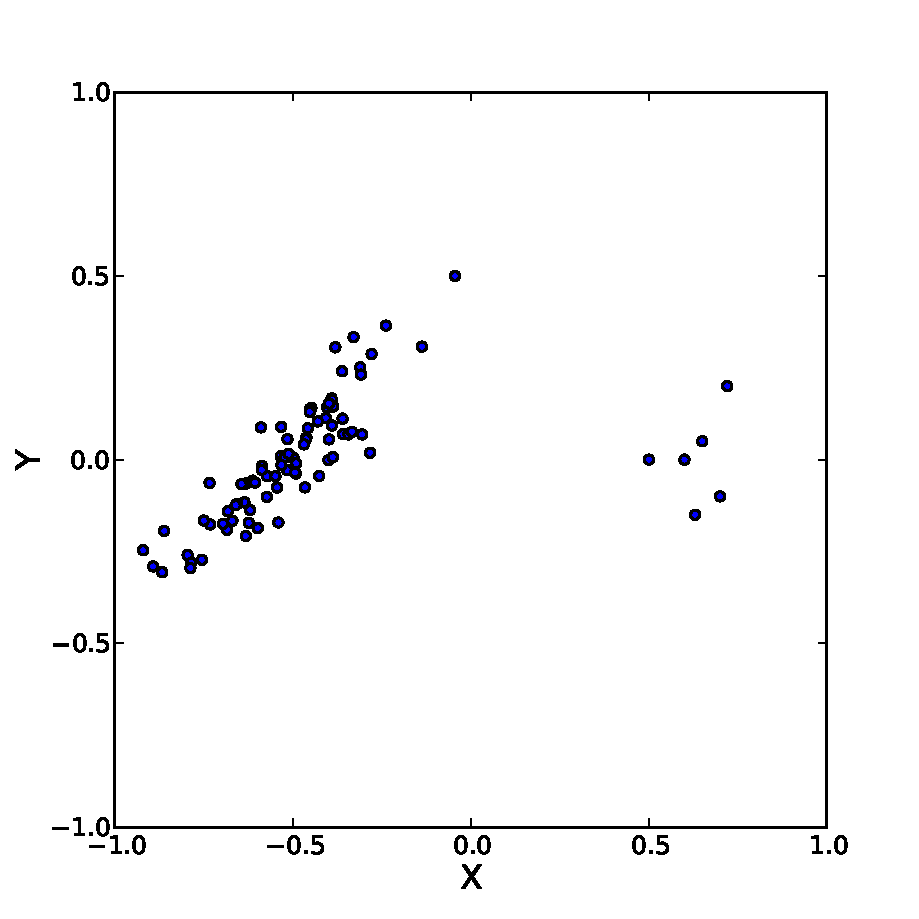
\includegraphics[width=\columnwidth]{../code/final_results/spearman_images/outliers.pdf}
  \caption{\begin{tabular}{r l}
 Pearson correlation: & 0.55\\
 p-value: & 0.0\\
 \hline
 Spearman correlation: & 0.81\\
 p-value: & 0.0
\end{tabular}}  \label{fig:outliers}
\end{subfigure}
\end{center}
\caption[Spearman's correlation coefficient -- outliers]{Spearman's rank correlation coefficient is less sensitive to outliers than Pearson's correlation coefficient, because each data point is first projected to its rank. For the above dataset, the Pearson's correlation coefficient is only 0.55, while Spearman's correlation coefficient is 0.81. Both correlations are statistically significant, since their p-values are below 0.05.}
\end{figure}


The Spearman's rank correlation coefficient or Spearman's rho, named after
Charles Spearman, is a non-parametric estimator of the statistical dependence of
two random variables \cite{lehman2005jmp}. It intuitively measures how well
the dependence between two variables can be measured using a monotonic function.
It is normally defined as follows:
\begin{mydef}
Let $X$ and $Y$ be two population samples and let $ x_i$ and $ y_i $ be the ranks of each of the data points in $X$ and $Y$. The Spearman's rank correlation coefficient is defined as the Pearson's correlation coefficient of the ranks $ x_i, y_i $ of the data points \emph{\cite{myers2010research}}.
\end{mydef}


\rowcolors{1}{blue1}{blue2}

\begin{table}
  \centering
  \begin{tabular}{ | c | c | c |}
    \hline
    \cellcolor{blue3} Variable $X_i$ & \cellcolor{blue3} Position & \cellcolor{blue3} Rank\\
    \hline
    0.3 & 1 & 1\\
    \hline
    0.6 & 2 & 2\\
    \hline
    1.2 & 4 & $ \frac{4+5}{2} $\\
    \hline
    1.2 & 5 & $ \frac{4+5}{2} $\\
    \hline
    0.8 & 3 & 3\\
    \hline
    1.9 & 6 & 1\\
    \hline
  \end{tabular}
  \caption{Computation of Spearman's ranks for a dataset of 6 samples. The data is initially sorted in ascending order. If the data point is
unique, then the rank is simply the position in the ordered list. Otherwise,
the rank is computed as the average of the positions of all the data points
with the same value.}
  \label{tab:ranks_table}
\end{table}

The calculation of the ranks is best illustrated in table \ref{tab:ranks_table}.
After the rank $ x_i, y_i $ of each data point is calculated,
the Spearman's correlation coefficient is computed using the formula for the Pearson's
correlation coefficient.


Spearman's correlation coefficient is considered non-parametric in the sense
that one does not need to know any prior on the $X$ and $Y$ random variables, as
it does not require knowledge (i.e.\ the parameters) of the joint probability
distribution of $X$ and $Y$.

\subsection{Computing the GDV correlation matrix of a network}
\label{pearsons_background}

We can use the Pearson's or Spearman's correlation coefficient previously
described to compute the \emph{GDV correlation matrix} for a given network in the
following manner:
\begin{enumerate}
 \item We compute the 73-element Graphlet Degree Vector (GDV) for every node in the
input network
 \item We then construct samples $ S_i, i\in {1,2,3, .. ,73} $
containing all the frequencies of the orbits of type $i$ found in the GDVs of
the nodes.
 \item We compute the Pearson's (or Spearman's) correlation coefficient of each
pair of samples $ (S_i, S_j) $ and we put them in the 73x73 correlation matrix $
C_{ij} $.
\end{enumerate}

The newly obtained graphlet correlation matrix will be symmetric with respect to 
the main diagonal, as Pearson's correlation coefficient is also symmetric. In
order to display such a matrix, we use a heat map, with blue representing a correlation of -1 and red representing a correlation of 1.

Given two matrices from two different networks $G$ and $H$, we then calculate
the \emph{Pearson's correlation matrix distance} between them by performing pairwise-subtractions of the elements. The \emph{Pearson's correlation matrix distance} is also referred to as the \emph{Graphlet correlation distance} in the literature \cite{yaverouglu2014revealing}.

\begin{mydef}
\label{def:gcd}
 Let $G$ and $H$ be two graphs and $G'$, $H'$ their Pearson's correlation matrices. The Pearson's correlation matrix distance or Graphlet correlation distance between $G$ and $H$ is then defined as:
 \begin{equation}
\label{pears_matrix_diff}
  D(G,H) = \sum_{i,j}\left(G'(i,j) - H'(i,j)\right)^2
\end{equation}
 
\end{mydef}

Note that the computed distance $D(G,H)$ is always greater than 0. We are now able to define the \emph{Graphlet Correlation Matrix Agreement}, which measures how similar two graphs are with respect to the GDV signatures.

\begin{mydef}
The \emph{Graphlet Correlation Matrix Agreement} between two graphs $G$ and $H$ is
defined as: 
 \begin{equation}
 Agreement = 1 - D(G,H)
 \end{equation}
\end{mydef}

One advantage of using the \emph{Graphlet Correlation Matrix Agreement} instead of the \emph{GDD agreement} previously defined is that it has been shown to be more robust to noise in the network data \cite{kuchaiev2009learning}.

\subsection{Hierarchical clustering}
\label{hier_clust}

When analysing the GDV correlation matrix of a network, we are interested to find out 
how graphlets group together with the rest of the graphlets according to their correlation. 
These groups of graphlets can be easily identified if we use \emph{hierarchical clustering}, 
which is a clustering method that builds a dendogram of the graphlets according to a distance function. 

The two main types of strategies for hierarchical clustering are:
\begin{itemize}
 \item Agglomerative (bottom-up): Each observation starts in its own cluster. At each step, the clusters with the smallest distance between each other are merged.  
 \item Divisive (top-down): All observations start in one cluster. At each step, the clusters are split recursively.
\end{itemize}

\subsubsection{Distance metric}
In order to perform \emph{hierarchical clustering}, a distance metric has to be defined. Some commonly-used metrics are:
\begin{itemize}
 \item Euclidean distance: $ \|a - b\|_2 = \sqrt{\sum_{i}(a_i - b_i)^2}$
 \item generalised p-norm: $ \|a - b\|_p = \left(\sum_{i}|a_i - b_i|^p\right)^\frac{1}{p}$
 \item Mahalanobis distance: $ \|a - b\| = \sqrt{(a - b)S^{-1}(a-b)}$, where $S$ is the covariance matrix
\end{itemize}


\subsubsection{Linkage criteria}

The linkage criteria defines the distance between the sets of data points as a function of the distances between the data points themselves. 

Some commonly used criteria for the linkage between two sets $A$ and $B$ are \cite{szekely2005hierarchical}:
\begin{itemize}
 \item Complete linkage clustering: $max \{d(a,b) | a \in A, b \in B\}$
 \item Single linkage clustering: $min \{d(a,b) | a \in A, b \in B\}$
 \item Average linkage clustering \cite{sokal1958statistical}: $max \{d(a,b) | a \in A, b \in B\}$
 \item Centroid linkage clustering: $ ||c_A - c_B|| $ where $c_A$ and $c_B$ are the centroids of clusters $A$ and $B$.
\end{itemize}


\section{Canonical Correlation Analysis}
\label{cca_background}

Canonical Correlation Analysis is a statistical method of analysing interdependence 
between two random variables $X$ and $Y$. The method was first introduced in 1936 by 
Harold Hotelling \cite{hotelling1936relations} and it has been used for 
analysing and interpreting data in various fields including 
Psychology \cite{cooley1971multivariate}, Marketing \cite{fader1990cross} and 
Operations Research \cite{pisharodi1991interset}.

Given two random variables $X$ and $Y$ and a set of vector weights $a_1$ and $b_1$, 
let $u_1 = Xb_1$ and $t_1 = Ya_1$. Canonical Correlation Analysis (CCA) aims to 
find the weights $a_1$ and $b_1$ such that the correlation $ \rho = r(t_1, u_1) $
is maximised. In this case, $u_1$ and $t_1$ are called the first canonical variates. 

The CCA process can be repeated again in order to find a second pair of canonical 
variates $u_2$ and $t_2$, with the additional condition that they are orthogonal to the first set 
of canonical variates $u_1$ and $t_1$. Thus, the second stage of the canonical correlation problem 
can be stated as follows:

Choose $a_2$,$b_2$ to maximise 
\begin{equation}
r(t_2, u_2) = r(Ya_2, Xb_2)
\end{equation}
such that 
$$r(t_1, t_2) = 0 \text{ and } r(u_1, u_2) = 0$$

This procedure can be repeatedly applied, although at each iteration the amount of correlation that we can achieve is decreasing. The reason for this is because each subsequent problem contains one extra orthogonality constraint compared to the previous one. The number of "stages" to the canonical correlation problem depends on the number of variables. 
If $p$ is the number of $X$ variables and $q$ is the number of $Y$ variables, then the maximum 
number of canonical variates that can be computed is $min(p,q)$.

\subsection{Derivation of Canonical Correlation Analysis}

We first define the correlation matrix $R$ as:

\rowcolors{1}{}{}

$$R = 
\begin{pmatrix}
R_{YY} & R_{YX} \\
R_{XY} & R_{XX} 
\end{pmatrix}
$$

where $R_{XY}$ is the correlation matrix between $X$ and $Y$, while $R_{XX}$ and $R_{YY}$ are the correlation matrices of $X$ and $Y$.  


We find that solving the problem in matrix form will in fact give the solution to all 
stages of the problem. Dropping the subscripts on variates $u = Xb$ and $t = Ya$, we restate the problem as follows:\\

Choose $a$, $b$ to maximise 

\begin{equation}
\label{cca_no_subscript}
r(t, u)=\frac{cov(t,u)}{\sqrt{var(t)var(u)}}
\end{equation}

The numerator of the objective function in equation (\ref{cca_no_subscript}) is simply given by:

$$Cov(t,u) = \frac{[t'u]}{n-1}=\frac{a'Y'Xb}{n-1} = a'R_{YX}b$$

By standardising $t$ and $u$, we effectively eliminate the denominator from the objective 
function in equation (\ref{cca_no_subscript}). Note that setting $ var(t) = 1 $ is equivalent to the following:
  
$$ var(t) = 1 $$
$$\implies \frac{[t't]}{n-1} = 1 $$
$$ \implies \frac{[a'Y'YA]}{n-1} = 1 $$
$$ \implies a'R_{YY}a = 1$$

Similarly, setting $var(u) = 1$ is the same as setting $b'R_{XX}b = 1$. Imposing these 
constraints, the problem becomes:\\

Choose $a$, $b$ to maximise 
$$a'R_{XX}b$$ 
subject to 
\begin{equation}
\label{cca_constraints}
a'R_{YY}a = 1 \text{ and } b'R_{XX}b = 1
\end{equation}

This constrained maximisation problem can be solved by using Lagrange multipliers and solving the first-order conditions. Using $\alpha/2$ and $\beta/2$ as Lagrange multipliers, the Lagrangian function is then given by:

\begin{equation}
 L = a'R_{YX}b - \frac{\alpha}{2}(a'R_{YY}a - 1) - \frac{\beta}{2}(b'R_{XX}b - 1) 
\end{equation}

Differentiating with respect to $a$ and $b$ and setting the results equal to zero gives the first-order necessary conditions:

\begin{equation}
\label{cca_foc1}
  \frac{\partial L}{\partial a} = 0 \implies R_{YX}b - \alpha R_{YY}a = 0
\end{equation}
\begin{equation}
\label{cca_foc2}
 \frac{\partial L}{\partial b} = 0 \implies R_{XY}a - \beta R_{XX}b = 0
\end{equation}

Taking the expression in equation (\ref{cca_foc1}) and premultiplying by $a'$ yields:

$$a'R_{YX}b - \alpha (a'R_{YY}a) = 0$$
which implies that $\alpha = r(t,u) $, the canonical correlation, because $a'R_{YY}a=1$ under the scaling constraints we have imposed for this problem. Similarly, taking equation (\ref{cca_foc2}) and premultiplying by $b'$ yields $\beta = r(t,u)$, which means that $\alpha = \beta$.

Now that the values of $\alpha$ and $\beta$ are known, we can substitute into equations (\ref{cca_foc1}) and (\ref{cca_foc2}) and solve the expressions for either $a$ or $b$.

Suppose we choose to solve for b. We use equation (\ref{cca_foc1}) to write $a$ as a function of $b$ as follows:

\begin{equation}
\label{cca_a}
  a = \frac{1}{r(t,u)}R^{-1}_{YY}R_{YX}b
\end{equation}

We then substitute the right-hand side of equation (\ref{cca_a}) above for $a$ in equation (\ref{cca_foc2}) and solve for $b$. The result is:

\begin{equation}
 R_{XY}\left( \frac{1}{r(t,u)}R^{-1}_{YY}R_{YX}b \right) = r(t,u)R_{XX}b
\end{equation}

Premultiplying by $R^{-1}_{XX}$ and mutiplying through by $r(t,u)$ gives:

\begin{equation}
  \label{cca_eigen_eq}
 [R^{-1}_{XX}R_{XY}R^{-1}_{YY}R_{YX}]b = r^2(t,u)b
\end{equation}

Equation (\ref{cca_eigen_eq}) is an eigenvector-eigenvalue problem. The vector $b$ is the first eigenvector of the matrix $R^{-1}_{XX}R_{XY}R^{-1}_{YY}R_{YX}$. The proportionality constant, which is the eigenvalue corresponding to $b$, is the squared canonical correlation $r^2(t,u)$. Although we will not prove this in the report, the structure of the canonical correlation problem ensures that the eigenvalues are both real and non-negative \cite{carroll1997mathematical}. 

We can now find $a$ by substituting $b$ into equation (\ref{cca_a}). We also find that $a$ is the first eigenvector of the matrix $R^{-1}_{YY}R_{YX}R^{-1}_{XX}R_{XY}$. The first eigenvalue is again the squared canonical correlation.

\subsection{Canonical Loadings}

To facilitate interpretation, it is helpful to look at canonical loadings, which are correlations between original variables and their corresponding canonical variates. The correlations between $X$ and $u$, which we denote $f$, are given by:

\begin{equation}
 f = \frac{1}{n-1}X'u = \frac{1}{n-1}X'(Xb) = R_{XX}b
\end{equation}
Similarly, the correlations between $Y$ and $t$, denoted $g$ are given by:
\begin{equation}
 g = \frac{1}{n-1}Y't = \frac{1}{n-1}Y'(Ya) = R_{YY}a
\end{equation}

\subsection{Canonical Cross-Loadings}

A slightly different concept is given by canonical cross-loadings, which are the correlations between original variables and the opposite canonical variates. The correlations between $X$ and $t$, which we denote $h$, are given by:

\begin{equation}
 h = \frac{1}{n-1}X't = \frac{1}{n-1}X'(Ya) = R_{XY}a
\end{equation}
The cross-loadings between $Y$ and $u$, denoted $j$ are given by:
\begin{equation}
 j = \frac{1}{n-1}Y'u = \frac{1}{n-1}Y'(Xb) = R_{YX}b
\end{equation}

In our project, when we present CCA results we only use canonical cross-loadings, because we are interested to find out how each element from one variate correlates with the elements from the opposite variate.

\subsection{Interpretation of Canonical Correlation Results}

The weights $a$ and $b$ that maximise the correlation $ \rho = corr(Xa, Yb) $ can be easily interpreted in the following manner:
\begin{itemize}
 \item If two values $a_i, b_j$ have the same sign it means that variables $X_i$, $Y_j$ are positively correlated. Similarly, if the values of $a_i, b_j$ have different signs then it means that the variables are negatively correlated. 
 \item A higher absolute value of $a_i$ and $b_j$ means that variables $X_i$, $Y_j$ show a stronger correlation. Similarly, if the absolute value of $a_i$ and $b_j$ is close to zero then it shows that variables $X_i$, $Y_j$ show a weak and insignificant correlation.
 \item If the weight vectors $a$ and $b$ are multiplied by scalars $\alpha$ and $\beta$ respectively, then the resulting correlation $ \rho' = corr(\alpha aX, \beta bY) $ is still the same as the original correlation between vectors $a$ and $b$, that is $ \rho = corr(Xa, Yb) $.
\end{itemize}

Note that in this report, when we say that two elements $x_i$ and $y_i$ of vectors $X$ and $Y$ correlate positively or have a positive correlation with respect to each other, it means that they have the same sign. Similarly, $x_i$ and $y_i$ will correlate negatively if they have opposite signs.

\section{Networks analysed}
\label{sec:networks_analysed}

Throughout the project we will be analysing several classes of networks:
\begin{itemize}
 \item Protein-Protein Interaction (PPI) networks
 \item Metabolic networks
 \item World Trade networks
%  \item Literature networks
\end{itemize}

 In order to perform Canonical Correlation Analysis, we have also used annotations, which are labels that offer information about each node in the graphs. For a country in the World Trade network (WTN), the annotations are financial indicators such as GDP per capita. On the other hand, for a protein in the PPI network these are properties such as "RNA transcription" or "energy production" that describe the function of the protein. Each of these networks and their annotations are described in detail in the following sections.

\subsection{Protein-Protein Interaction networks}
\label{sec:ppi_bck}

The Protein-Protein Interaction networks, or PPI networks are mainly represented by a graph where the nodes are proteins and the edges are interactions between proteins. These interactions are normally captured using technologies such as \emph{Yeast two-hybrid screening} \cite{young1998yeast} or \emph{affinity purification mass spectrometry} (AP-MS) \cite{brettner2012protein,wodak2013protein}.

The source of our PPI networks is the \emph{Biological General Repository for Interaction Datasets} (BioGRID). Throughout the project we have mainly focused on the Human PPI network, although some of our experiments have also been performed on the PPI networks of other model organisms such as C. elegans(worm), D. melanogaster(fruit fly), E. coli(bacteria), M. musculus(mouse) and S. cerevisiae(baker's yeast). We have done this in order to find out whether our results are consistent across a spectrum of networks from different species.

\subsubsection{Annotations}
\label{ppi_annotations}

In order to assign functional information to each protein in the PPI network, we have used \emph{Gene Ontology terms}, commonly called \emph{GO terms}. These are part of a large project called \emph{Gene Ontology} that aims to unify the representation of gene attributes across all species \cite{gene2008gene}. Moreover, we have also used two smaller annotation sets that only contained 13 and 14 functional terms respectively. The first one belongs to Christian von Mering et al. \cite{von2002comparative} and contains the following annotations:
\begin{multicols}{2}
\begin{itemize}
  \item Energy production
  \item Amino acid metabolism
  \item Other metabolism
  \item Translation
  \item Transcription
  \item Transcriptional control
  \item Protein fate
  \item Cellular organisation
  \item Transport and sensing
  \item Stress and defence
  \item Genome maintenance
  \item Cellular fate / organisation
  \item Uncharacterized
\end{itemize}
\end{multicols}

The second annotation file is from Charlie Boone \cite{costanzo2010genetic} and contains a slightly different annotation set:
\begin{multicols}{2}
\begin{itemize}
  \item Golgi endosome vacuole sorting
  \item Metabolism - mitochondria
  \item DNA replication
  \item Chromatin transcription
  \item Cell polarity morphogenesis
  \item Signalling stress response
  \item Chromatin  segmentation
  \item Protein folding
  \item ER Golgi traffic
  \item Nuclear cytoplasmic transport
  \item Cell cycle progression meiosis
  \item Protein degradation proteosome
  \item RNA processing
  \item Ribosome translation
\end{itemize}
\end{multicols}

Nevertheless, both annotation files label each proteins according to their function. Since these annotation sets are more compact\footnote{GO terms are in the order of thousands. A more compact version called GO Slim exists, which has around 100 different functional annotations.} than GO terms, we have found it easier to work with Boone's and von Mering's annotation files.

\rowcolors{1}{blue1}{blue2}

\begin{table}
  \centering
  Basic statistics of the Human PPI network\\
  \begin{tabular}{  c  c | c  c }
%     \hline
    Clustering coefficient & 0.125 & Number of nodes & 11099\\
    Connected components & 77 & Density & 0.001\\
    Network diameter & 13 & Heterogeneity & 1.945\\
    Average number of neighbours & 10.236 & Isolated nodes & 0\\
    Network centralisation & 0.046 & Number of self-loops & 0\\
    Shortest paths & 119,301,268 (96\%) & Multi-edge node pairs & 0\\
    Characteristic path length & 3.963 & Edges & 56806\\
%     \hline
  \end{tabular}
  \caption{Basic statistics for the Human PPI network. The Human PPI network has a large number of nodes (11099), a small clustering coefficient (0.125) and a large network diameter (13).}
  \label{tab:ppi_stats_table}
\end{table}

\subsection{Metabolic networks}
\label{sec:meta_bck}

A metabolic network is a set of chemical and metabolic processes that regulate physiological and biochemical properties of a cell. Therefore, these networks contain metabolic pathways and regulatory interactions that guide these processes. The source of our metabolic network data and annotations is the \emph{Kyoto Encyclopedia of Genes and Genomes} (KEGG) \cite{kegg}. Other sources where metabolic networks are available include \emph{EcoCyc} \cite{ecocyc} and \emph{BioCyc} \cite{biocyc}.

Throughout the project we have analysed two main types of metabolic networks:
\begin{itemize}
 \item Enzyme-based metabolic networks: each node in the network graph corresponds to an enzyme, protein, metabolite or other chemical. An edge is constructed whenever two chemicals participate in the same reaction.
 \item Compound-based metabolic networks: each node in the network graph is a compound, which is a set of enzymes that usually take part in one reaction of the metabolic process. In the compound-based networks, edges are formed between compounds as opposed to individual enzymes.
\end{itemize}

\subsubsection{Annotations}
\label{metabolic_annotations}

The two types of metabolic networks can be annotated with functional information about the enzymes or compounds respectively. One annotation set we used is the Enzyme Commission number, which is a numerical classification for enzymes that is based on the chemical reactions they catalyse \cite{webb1992enzyme}. Every enzyme code consists of four numbers separated by periods. When annotating the enzymes from our metabolic networks we have only used the top-level EC numbers:
\begin{enumerate}
 \item \textbf{Oxidoreductases}: enzymes that catalyse the transfer of electrons from one molecule to another.
 \item \textbf{Transferases}: enzymes that enact the transfer of specific functional groups (e.g. a methyl or glycosyl group) from one molecule to another.
 \item \textbf{Hydrolases}: enzymes that catalyse the hydrolysis\footnote{Hydrolysis is a chemical process in which chemical bonds are broken by the addition of water.} of a chemical bond.
 \item \textbf{Lyases}: enzymes that catalyse the breaking of various chemical bonds by means other than hydrolysis.
 \item \textbf{Isomerases}: enzymes that convert a molecule from one isomer to another.
 \item \textbf{Ligases}\footnote{from the Latin verb ligare: "to bind" or "to glue together"}: enzymes that catalyse the joining of two large molecules by forming a new chemical bond.
\end{enumerate}


\begin{table}
  \centering
  Basic statistics of the Human Metabolic network\\
  \begin{tabular}{  c  c | c  c }
    Clust coeff & 0.251 & Nr of nodes & 1343\\
    Connected components & 2 & Density & 0.005\\ 
    Network diameter & 9 & Heterogeneity & 2.702\\
    Avg. nr of neighbours & 6.774 & Isolated nodes & 0\\
    Network centralisation & 0.322 & Number of self-loops & 26\\
    Shortest paths & 1,796,942 (99\%) & Multi-edge node pairs & 1127\\
    Characteristic path length & 3.362 & Edges & 8610\\
  \end{tabular}
  \caption{Basic statistics for the Human Metabolic network. In terms of node size, the Human Metabolic network lies somewhere in between the PPI network and the World Trade network. It also has a medium clustering coefficient (0.251) and small density (0.005). }
  \label{tab:meta_stats_table}
\end{table}


% in trade also include thresholding method
\subsection{World Trade Networks}
\label{sec:trade_bck}

The \emph{World Trade network} (WTN), commonly called the trade or economic network in this report, contains a set of countries and the corresponding trade volume in commodities between them in a particular year. The volume of trade is expressed in international dollars (\$). The data has been taken from the \emph{United Nations Commodity Trade} website (Comtrade) \cite{comtrade}. The data that is available on the website is given as an undirected edge-list file, where each edge is weighted by the volume of trade between those two countries. Moreover, the edge list is sorted by the weight, with the countries that traded most with each other at the top of the list.

Since most of the countries trade with each other at least in small or negligible amounts, the original network graph is very dense. In order to reduce the density of the network and analyse only the important economic links between countries, the network has been thresholded to an 85\% level. This means that only the highest-weighted edges that made up 85\% of the total trade were finally kept, with the rest being discarded. As a result of this thresholding operation, we only kept the countries that trade significantly with each other.

We have analysed data from 49 different WTNs for all years between 1962 and 2010. Having this time series data allowed us to find patterns in the changes of world trade as it evolves over time. Table \ref{tab:trade_stats_table} shows basic statistics for the 2010 trade network - thresholded at the 85\% level. Moreover, apart from total trade network, we have also worked with the following commodity-specific trade networks:
\begin{itemize}
 \item Minerals and fuels
 \item Food and live animals
\end{itemize}

These networks represent the trade in a specific commodity that was done throughout the world. Table \ref{tab:trade_stats_table} shows basic statistics for the 2010 WTN. One can notice that the diameter of the network is really small (0.4). This is slightly undesirable, because the smaller the diameter the stronger the GCV correlation will be between nodes, because the probability of two nodes sharing part of their neighbourhood is large. Therefore, we tried thresholding the network at levels lower than 85\%, in order to make the network more disconnected and therefore increase its diameter. However, this attempt has not succeeded, because the network diameter has stayed at the same level. The reason for this might be because of the scale-free properties of the network, which ensure that when thresholding is applied, the isolated nodes are removed and only hub nodes are kept.

\begin{table}
  \centering
  Basic statistics of the 2010 World Trade Network\\
  \begin{tabular}{  c  c | c  c }
    Clust coeff & 0.583 & Nr of nodes & 119\\
    Connected components & 1 & Density & 0.110\\
    Network diameter & 4 & Heterogeneity & 1.255\\
    Avg. nr of neighbours & 12.992 & Isolated nodes & 0\\
    Network centralisation & 0.578 & Number of self-loops & 0\\
    Shortest paths & 14,042 (100\%) & Multi-edge node pairs & 0\\
    Characteristic path length & 2.137 & Edges & 773 \\
  \end{tabular}
  \caption{Basic statistics for the 2010 World Trade network that has been thresholded at the 85\% level. The network has a small number of nodes(119), large clustering coefficient(0.583) and small network diameter(4).}
  \label{tab:trade_stats_table}
\end{table}

\subsubsection{Annotations - Economic indicators}

The basic economic indicators that we have used for the Canonical Correlation analysis are the following:
\begin{itemize}
 \item Population (POP): The total population of the country. Data source: WEO \cite{weo2014}
 \item Level of Employment (LE): The number of people who performed some work during a specified period. Data source: WEO \cite{weo2014}.
 \item Real GDP per capita (RGDPL): Purchasing Power Parity adjusted Gross Domestic Product (Laspeyres) which was derived from the growth rates of consumption share, government share and investment share. Data source: PENN \cite{heston2002penn}
 \item Real GDP per capita (RGDPL2) -- Purchasing Power Parity adjusted Gross Domestic Product (Laspeyres) which was derived from the growth rates of domestic absorption. Data source: PENN \cite{heston2002penn}
 \item Real GDP per capita -- Constant Prices Chain series (RGDPCH). Data source: PENN \cite{heston2002penn}
 \item Consumption Share of RGDPL (KC) -- Data source: PENN \cite{heston2002penn}
 \item Government Share of RGDPL (KG) -- Data source: PENN \cite{heston2002penn}
 \item Investment Share of RGDPL (KI) -- Data source: PENN \cite{heston2002penn}
 \item Exchange Rate (XRAT) -- Data source: PENN \cite{heston2002penn}
 \item Current Account Balance (BCA): The difference between a country's exports of goods and services and its imports. Financial transfers and investments are not taken into account. Data source: PENN \cite{heston2002penn}
 \item Trade Openness (OPENK) -- Data source: PENN \cite{heston2002penn}
\end{itemize}

Moreover, this list of economic indicators has been augmented with composed indicators that are the products of several basic indicators. The full list is as follows:
\begin{multicols}{3}
\begin{itemize}
  \item POP 
  \item LE
  \item KI x RGDPL x POP
  \item RGDPCH x POP
  \item RGDPL x POP
  \item RGDPL2 x POP
  \item KG x RGDPL x POP
  \item KC x RGDPL x POP
  \item KC x RGDPL
  \item XRAT 
  \item RGDPCH
  \item RGDPL 
  \item RGDPL2
  \item KG x RGDPL
  \item KI x RGDPL
  \item KC
  \item KI
  \item BCA per RGDPL
  \item KG
  \item BCA
  \item OPENK
\end{itemize}
\end{multicols}



% Chapter 3
\chapter{Methodology}
\label{chp:methodology}
%You are free to write up any additional material that will appear in the final
%report, for example a section or chapter describing a significant component of
%the design/implementation that you have already completed.  Avoid any
%additional material that is not re-usable in the final report.

\section{Mathematical model}
\label{sec:math_model}

We now introduce the novel signature that can be interpreted as a generalisation of
the \emph{Graphlet Distribution Vector} (GDV) described in section \ref{sec:gdv}. This signature, which we shall call the \emph{Graphlet Cluster Vector} (GCV) (for reasons that will soon become obvious), is a central concept of this project. Since the GCV is a novel signature, we would like to explore its properties and find out how to use it for getting insights from the network data. The idea for the novel GCV signatures came from Zoran Levnaji\'{c}, one of Nata\v{s}a Pr\v{z}ulj's collaborators. Before giving a full definition of the GCV, we first define what the \emph{neighbouring subgraph} of a node $n$ is: 

\begin{mydef}
\label{def:neighbouring_subgraph}
 Let $G = (V,E)$ be a graph and $n$ be a node in $V$. The neighbouring subgraph $S_n=(V_n,E_n)$ of node $n$ is an induced subgraph of $G$ where $V_n$ is the set of all neighbouring vertices of $n$, with $n \notin V_n$.
\end{mydef}

This implies that $S_n$ will contain all the edges between the neighbours of $n$ excluding those coming from the source node $n$ itself. Now that we have defined the neighbouring subgraph of a node, we are ready to give the full definition of the new \emph{Graphlet Cluster Vector}:
\begin{mydef}
\label{def:unnorm_gcv}
 Let $G$ be a graph, $n$ a node in $G$, \( S_n \) the neighbouring subgraph of $n$ in $G$ and let \( S_n^i\) be the number of graphlets of type i in \( S_n \), $i \in \{1,2, \dots 29\}$. The Graphlet Cluster Vector of node $n$ is a vector of 29 elements defined as:
 $$ GCV(n) = \left(S_n^1, S_n^2, \dots , S_n^{29}\right)$$
\end{mydef}

The GCV signature of a node $n$ is therefore counting the number of graphlets of each type in $n$'s neighbouring subgraph. One can also normalise it with respect to the total number of graphlets found in $S_n$ to get the \emph{normalised Graphlet Cluster Vector}. The formal definition is the following:

\begin{mydef}
\label{def:norm_gcv}
 Let $G$ be a graph, $n$ a node in $G$, \( S_n \) the neighbouring subgraph of $n$ in $G$ and let \( S_n^i\) be the number of graphlets of type i in \( S_n \). The normalised Graphlet Cluster Vector of node $n$ is defined as:
 $$ GCV(n) = \left(F_n^1, F_n^2, ... F_n^{29}\right)$$
 where
 $$ F_n^i = \frac{S_n^i}{\sum_{i=1}^{n}S_n^i} $$
\end{mydef}

There are several ways to interpret both variants of the GCV signature:
\begin{itemize}
 \item GCV generalises the GDV by capturing structural information in the neighbouring subgraph of a particular node. The GDV used to count the number of graphlets touching a node at a particular orbit. 
 \item In the normalised version, if the GCV would have also recorded the frequency of graphlet $G_0$\footnote{$G_0$ is simply an edge between two nodes.}, that frequency would have represented the clustering coefficient of node $n$. Therefore, one can also interpret the GCV as a generalisation of the clustering coefficient of a node.
 \item The normalised version of the GCV of a node $n$ can also be interpreted as an exponentiated\footnote{RGFV applies a logarithmic function to each of the frequencies, see definition \ref{def:rgfv} in section \ref{sec:graphlets}} RGFV\footnote{RGFV counts the frequency of graphlets in the whole graph, see definition \ref{def:rgfv} in section \ref{sec:graphlets}} of the neighbouring graph of node $n$.
\end{itemize}

The reason we don't include graphlet $G_0$ is because that simply gives us the clustering coefficient of the node. Moreover, $G_0$ correlates positively with all the other graphlets in the vector, since it is a subgraph of all the other graphlets. Therefore, that does not give us any useful information in Pearson's GCV correlation matrices or CCA. 

As it was previously mentioned, the core idea of the GCV signature belongs to Dr. Zoran Levnaji\'{c}, one of Nata\v{s}a Pr\v{z}ulj's collaborators. Nevertheless, I also have some contributions to the mathematical model, because at the beginning of the project I researched a few normalisation methods and sizes of the neighbouring subgraph of a node where the GCV is calculated. After several normalisation procedures and neighbouring subgraph sizes have been discussed and analysed, we decided on the version presented in this paper. For an overview of a different normalisation method attempted, see section \ref{sec:gcv_norm_attempt}. For a study on the neighbouring subgraph size, see section \ref{sec:neigh_subgr_size}.

\begin{figure} 
\centering
\begin{tikzpicture}[scale=1.5,auto,swap]

  \draw (-2,0) ellipse (0.85cm and 1.8cm);
  \node[upper left] at (current bounding box.north east) {\textbf{$S_1$}};	
  
  % define the round nodes
  \node[vertex,blue] (1a) at (-3.75877048314363,0) {$1$};
  
  \foreach \pos/\name/\label in {
    {(-2.0,1.46)/2/2a},
    {(-2.5,0.5)/3/3a},
    {(-1.5,-0.5)/4/4a},
    {(-2.0,-1.46)/5/5a},
    {(0.5,-0.46)/6/6a}}
    \node[vertex] (\label) at \pos {$\name$} ;

    \node[upper left,inner sep=0] (src_lab) at (-4.5,0.75) {\rowcolors{1}{}{}\begin{tabular}{r} source\\ node \end{tabular}};
    \draw[->, thick]  (src_lab)  -- (1a) {}; 
    
  %neighbouring graph
	
  \path[hi, line width=1.0]  (4a)  -- (3a);
  \path[hi, line width=1.0]  (2a)  -- (4a);
  \path[hi, line width=1.0]  (5a)  -- (4a);
  
  % rest of edges, dotted

  \path[lo, line width=1.0]  (1a)  -- (2a);
  \path[lo, line width=1.0]  (1a)  -- (3a);
  \path[lo, line width=1.0]  (1a)  -- (4a);
  \path[lo, line width=1.0]  (1a)  -- (5a);
  \path[lo, line width=1.0]  (6a)  -- (5a);
\end{tikzpicture}
\caption[Illustration of the neighbouring of a node]{Illustration of the neighbouring subgraph $S_1$ of node 1. $S_1$ is made of 4 nodes: \{2,3,4,5\} and 3 edges: \{$(2,4)$,$(3,4)$,$(4,5)$\}. In order to find the GCV signature we count the frequency of graphlets of each type in $S_1$. In this example we obtain: $(3,3,0,1,0,0,0,...)$. Note that since there is no edge between nodes $1$ and $6$, node $6$ is not used for calculating the GCV of node $1$. Moreover, source node 1 and the edges linking it are also excluded from $S_1$.}
\end{figure}


\subsection{GCV normalisation attempt}
\label{sec:gcv_norm_attempt}

Our initial plan was to normalise each frequency in the GCV signature according to the maximum possible number of graphlets of that type in the neighbouring subgraph. However, this proved to be a very complicated mathematical problem, because both of the following sub-problems are mathematically non-trivial:
\begin{enumerate}
 \item Finding out which graphs contain the maximal number of graphlets of each type.
 \item Once such a graph is found, finding the formula for the maximum number of graphlets.
\end{enumerate}

Each of the above subproblems are unique for all the 30 different graphlets and they have to be solved separately. One remark we can make is that an upper limit for the maximum number of graphlets of type $i$ is :
$$ max(i) = {n \choose k} = \frac{n!}{k! (n-k)!} $$ 
where $i \in \{1,2, \dots 29\}$ and $k$ is the number of nodes in graphlet $i$.

For the first subproblem, one can hypothesise a graph structure that might have the maximal frequency of graphlet $i$ for a fixed number of nodes $n$ and mathematically prove that no other graph with the same number of nodes can yield a higher frequency. To illustrate the complexity of the problem, let us find the maximum number of graphlets of type 1 ($G_1$, path of 3 nodes) in a graph $H=(V,E)$, where $|V| = n$, for a given $n$. First of all, we need to identify which graph $H$ gives a high frequency of graphlet $G_1$. Since $G_1$ is not a clique, it would not be convenient for $H$ to be a clique either, otherwise the frequency of $G_1$ would be 0. Similarly, if $H$ has no edges, then the frequency of $G_1$ is also 0. 

One type of graph $H$ that might give us a high frequency of $G_1$ is a bipartite graph. Moreover, let us also assume that the nodes of $H$ are split into two sets of equal cardinality\footnote{If $n$ is odd then one extra node is added in $H_1$.} $H_1$ and $H_2$. Since we would like $H$ to be bipartite, let us assume edges exist between all nodes $i$ and $j$, with $i \in H_1$ and $j \in H_2$. Now that we have a candidate graph $H$ that might give us a high frequency of $G_1$ graphlets, one can count how many graphlets $G_1$ there are in $H$. The exact frequencies are given below:

\rowcolors{1}{}{}	
$$max(G_1, H) = \begin{cases}
   n^2(n-2)/8  & \text{if } n \text{ is even} \\
   x(x+1)(2x-1)/2 \text{ where } x = \floor{\frac{n}{2}} & \text{if } n \text{ is odd}
  \end{cases}$$
Therefore, this is the hypothesised maximum number of graphlets of type $G_1$ in a graph $H$ of $n$ nodes. The formulae already look complicated and get even more complex as the graphlets increase in size and density. Therefore, the problem of finding the maximum theoretical number of graphlets of each type is infeasible, at least for the purposes of our project. We have therefore decided to only normalise the GCV with the sum of all the frequencies, as it is given in definition \ref{def:norm_gcv} in the previous section.


\subsection{Study on neighbouring subgraph size}
\label{sec:neigh_subgr_size}

One other aspect that has been closely studied is the size of the neighbourhood subgraph. The current definition of the GCV uses a subgraph that excludes the source node and nodes that are at a distance of 2 or more from the source node. However, the subgraph can be extended in two different manners:
\begin{itemize}
 \item \textbf{Shell extension}: For a given parameter $d$, the neighbouring subgraph $S_n$ of a node $n$ contains nodes that are at a distance $d$ from $n$, where the distance between two nodes is defined as the minimum path length.
 \item \textbf{Core extension}: For a given parameter $d$, the neighbouring subgraph $S_n$ of a node $n$ contains all nodes that are at a distance $d$ or smaller from $n$. Moreover, $n \in S_n $.
\end{itemize}

Figure \ref{fig:shell_core} illustrates different shell and core neighbouring subgraphs for a source node. There are several  problems associated with shell and core neighbourhoods that are larger than 1:
\begin{itemize}
 \item The GCV computation becomes intractable for large networks, because the neighbourhood of each node is bigger.
 \item Finding the actual neighbourhood requires graph searching in order to find the shortest path between the source node and every other node in the network. This places further computational demand on the algorithm.
 \item Some networks such as the World Trade Networks have a short diameter of approximately 5. Therefore, the core-5 neighbourhood will contain all the nodes in the network, while core-4 and core-3 will also contain a lot of nodes if the starting node is a hub node.
\end{itemize}


\begin{figure}[H]
\centering
  \begin{subfigure}[b]{0.45\textwidth}
    \begin{tikzpicture}[scale=1.2,auto,swap]

      \draw (1.5,0) ellipse (0.7cm and 1.7cm);
%       \node[upper left] at (current bounding box.north east) {\textbf{$S_1$}};	
      
      \node[vertex,blue] (1a) at (0,0) {$1$};
      
      % define the round nodes
      \foreach \pos/\name/\label in {
	{(1.5,0)//2a},
	{(1.5,1)//3a},
	{(1.5,-1)//4a},
	{(3,0)//5a},
	{(3,2)//6a},
	{(3,-2)//7a}}
	\node[vertex] (\label) at \pos {$\name$} ;
  
      \node[upper left,inner sep=0] (src_lab) at (-1.5,0.75) {\begin{tabular}{r} source\\ node \end{tabular}};
      \draw[->, thick]  (src_lab)  -- (1a) {}; 
	
      %neighbouring graph
	    
      \path[lo, line width=1.0]  (1a)  -- (2a);
      \path[lo, line width=1.0]  (1a)  -- (3a);
      \path[lo, line width=1.0]  (1a)  -- (4a);
      \path[hi, line width=1.0]  (2a)  -- (4a);
      \path[lo, line width=1.0]  (3a)  -- (6a);
      \path[lo, line width=1.0]  (3a)  -- (5a);
      \path[lo, line width=1.0]  (4a)  -- (7a);   
      \path[lo, line width=1.0]  (5a)  -- (7a); 
      \path[lo, line width=1.0]  (5a)  -- (6a); 
      % rest of edges, dotted

%       \path[lo, line width=1.0]  (1a)  -- (2a);
%       \path[lo, line width=1.0]  (1a)  -- (3a);
%       \path[lo, line width=1.0]  (1a)  -- (4a);
%       \path[lo, line width=1.0]  (1a)  -- (5a);
%       \path[lo, line width=1.0]  (6a)  -- (5a);
    \end{tikzpicture}
    \caption{Shell-1 neighbourhood}
    \vspace{1em}  
  \label{fig:shell1}
  \end{subfigure}
  \begin{subfigure}[b]{0.45\textwidth}
    \begin{tikzpicture}[scale=1.2,auto,swap]

      \draw (3,0) ellipse (0.7cm and 2.5cm);
%       \node[upper left] at (current bounding box.north east) {\textbf{$S_1$}};	
      
      \node[vertex,blue] (1a) at (0,0) {$1$};
      
      % define the round nodes
      \foreach \pos/\name/\label in {
	{(1.5,0)//2a},
	{(1.5,1)//3a},
	{(1.5,-1)//4a},
	{(3,0)//5a},
	{(3,2)//6a},
	{(3,-2)//7a}}
	\node[vertex] (\label) at \pos {$\name$} ;
  
      \node[upper left,inner sep=0] (src_lab) at (-1.5,0.75) {\begin{tabular}{r} source\\ node \end{tabular}};
      \draw[->, thick]  (src_lab)  -- (1a) {}; 
	
      %neighbouring graph
	    
      \path[lo, line width=1.0]  (1a)  -- (2a);
      \path[lo, line width=1.0]  (1a)  -- (3a);
      \path[lo, line width=1.0]  (1a)  -- (4a);
      \path[lo, line width=1.0]  (2a)  -- (4a);
      \path[lo, line width=1.0]  (3a)  -- (6a);
      \path[lo, line width=1.0]  (3a)  -- (5a);
      \path[lo, line width=1.0]  (4a)  -- (7a);   
      \path[hi, line width=1.0]  (5a)  -- (7a); 
      \path[hi, line width=1.0]  (5a)  -- (6a); 
      % rest of edges, dotted

%       \path[lo, line width=1.0]  (1a)  -- (2a);
%       \path[lo, line width=1.0]  (1a)  -- (3a);
%       \path[lo, line width=1.0]  (1a)  -- (4a);
%       \path[lo, line width=1.0]  (1a)  -- (5a);
%       \path[lo, line width=1.0]  (6a)  -- (5a);
    \end{tikzpicture}
    \caption{Shell-2 neighbourhood} 
    \vspace{1em}  
    \label{fig:shell2}
  \end{subfigure}
  \begin{subfigure}[b]{0.45\textwidth}
    \begin{tikzpicture}[scale=1.2,auto,swap]

      \draw (0.8,0) ellipse (1.3cm and 1.8cm);
%       \node[upper left] at (current bounding box.north east) {\textbf{$S_1$}};	
      
      \node[vertex,blue] (1a) at (0,0) {$1$};
      
      % define the round nodes
      \foreach \pos/\name/\label in {
	{(1.5,0)//2a},
	{(1.5,1)//3a},
	{(1.5,-1)//4a},
	{(3,0)//5a},
	{(3,2)//6a},
	{(3,-2)//7a}}
	\node[vertex] (\label) at \pos {$\name$} ;
  
      \node[upper left,inner sep=0] (src_lab) at (-1.5,0.75) {\begin{tabular}{r} source\\ node \end{tabular}};
	
      %neighbouring graph
	    
      \path[hi, line width=1.0]  (1a)  -- (2a);
      \path[hi, line width=1.0]  (1a)  -- (3a);
      \path[hi, line width=1.0]  (1a)  -- (4a);
      \path[hi, line width=1.0]  (2a)  -- (4a);
      \path[lo, line width=1.0]  (3a)  -- (6a);
      \path[lo, line width=1.0]  (3a)  -- (5a);
      \path[lo, line width=1.0]  (4a)  -- (7a);   
      \path[lo, line width=1.0]  (5a)  -- (7a); 
      \path[lo, line width=1.0]  (5a)  -- (6a); 
      \draw[->, thick]  (src_lab)  -- (1a) {}; 
%       \draw[line,thick, ->] (file1) -- (file_final.north west) {};
      % rest of edges, dotted

%       \path[lo, line width=1.0]  (1a)  -- (2a);
%       \path[lo, line width=1.0]  (1a)  -- (3a);
%       \path[lo, line width=1.0]  (1a)  -- (4a);
%       \path[lo, line width=1.0]  (1a)  -- (5a);
%       \path[lo, line width=1.0]  (6a)  -- (5a);
    \end{tikzpicture}
    \caption{Core-1 neighbourhood}  
    \label{fig:core1}
  \end{subfigure}
    \begin{subfigure}[b]{0.45\textwidth}
    \begin{tikzpicture}[scale=1.2,auto,swap]

      \draw (1.9,0) ellipse (2.4cm and 2.6cm);
%       \node[upper left] at (current bounding box.north east) {\textbf{$S_1$}};	
      
      \node[vertex,blue] (1a) at (0,0) {$1$};
      
      % define the round nodes
      \foreach \pos/\name/\label in {
	{(1.5,0)//2a},
	{(1.5,1)//3a},
	{(1.5,-1)//4a},
	{(3,0)//5a},
	{(3,2)//6a},
	{(3,-2)//7a}}
	\node[vertex] (\label) at \pos {$\name$} ;
  
	
      %neighbouring graph
	    
      \path[hi, line width=1.0]  (1a)  -- (2a);
      \path[hi, line width=1.0]  (1a)  -- (3a);
      \path[hi, line width=1.0]  (1a)  -- (4a);
      \path[hi, line width=1.0]  (2a)  -- (4a);
      \path[hi, line width=1.0]  (3a)  -- (6a);
      \path[hi, line width=1.0]  (3a)  -- (5a);
      \path[hi, line width=1.0]  (4a)  -- (7a);   
      \path[hi, line width=1.0]  (5a)  -- (7a); 
      \path[hi, line width=1.0]  (5a)  -- (6a); 

      \node[upper left,inner sep=0] (src_lab) at (-1.5,0.75) {\begin{tabular}{r} source\\ node \end{tabular}};
      \draw[->, thick]  (src_lab)  -- (1a) {}; 
%       \draw[line,thick, ->] (file1) -- (file_final.north west) {};
      % rest of edges, dotted

%       \path[lo, line width=1.0]  (1a)  -- (2a);
%       \path[lo, line width=1.0]  (1a)  -- (3a);
%       \path[lo, line width=1.0]  (1a)  -- (4a);
%       \path[lo, line width=1.0]  (1a)  -- (5a);
%       \path[lo, line width=1.0]  (6a)  -- (5a);
    \end{tikzpicture}
    \caption{Core-2 neighbourhood} 
    \label{fig:core2}
  \end{subfigure}
\caption[Shell and Core neighbourhoods]{Shell and Core neighbourhoods for source node 1: (\subref{fig:shell1}) Shell-1 is the subgraph of nodes at distance 1 from the source node. (\subref{fig:shell2}) Shell-2 is the subgraph of nodes at distance 2 from the source node. (\subref{fig:core1}) Core-1 is the subgraph of nodes at distance 1 or smaller from the source node (including the source node itself). (\subref{fig:core2}) Core-2 is the subgraph of nodes at distance 2 or smaller from the source node (including the source node itself).}
\label{fig:shell_core}
\end{figure}

Because of these reasons we have decided against the use of core and shell neighbourhoods that have a size larger than 1. This left us only with core-1 and shell-1. The final decision was to use shell-1 because the resulting GCV signature would not count any graphlets that the older GCV signature would count as well. With core-1, there exist graphlets that touch the source node which are also counted by the other GDV signature. 

\subsection{Relative Cluster Frequency Distance}
\label{rcfd}

We now define the \emph{Relative Cluster Frequency Distance} (RCFD), which measures the distance between two GCVs. It is the equivalent of RGFD (section \ref{sec:rgfd}), but instead uses the GCV instead of the GDV.

\begin{mydef}
 Let $G$ be a graph, $p$ and $q$ two nodes in $G$ and let \(F_p^i\)
and \(F_q^i\) be the frequency of the $i^{th}$ graphlet in the GCVs of nodes $p$ and $q$ respectively. The Relative Cluster Frequency Distance (RCFD) between $p$ and $q$ is then defined as:
\begin{equation}
 RCFD(p,q) = \sqrt{\sum_{i=1}^{n}| F_p^i - F_q^i |^2}
\end{equation}
\end{mydef}

Note that the RCFD formula uses the Euclidean-distance, while the RGDF uses the absolute value as the distance measure. In this project, we use the Euclidean distance version for computing the RCFD.

\section{Implementation}

After the mathematical model behind the Graphlet Cluster Vector has been formally defined, we implemented it in \verb!C++!. The two main reasons for choosing \verb!C++! are as follows:
\begin{enumerate}
 \item Nata\v{s}a Pr\v{z}ulj's research group already wrote a \verb!C++! function that counted the number of graphlets in a given input graph. Therefore, we were able to leverage that code and add extra functionality on top of it.
 \item \verb!C++! is a compiled language that does not run in a virtual
environment, and consequently it can run intensive computations very fast. A similar implementation in a language such as Java, which runs on a virtual machine, takes longer. Since our algorithm is required to execute intensive computations on large biological networks, we decided that \verb!C++! was the most suitable programming language for this.
\end{enumerate}

The \verb!C++! file that I was given from N. Przulj's group (called ncount.cpp) was used to count both the RGFV (i.e.\ the number of graphlets of each type in a graph) and also the GDV signatures (i.e.\ the number of automorphism orbits that nodes touch). I was also given another script that was used to convert the given networks\footnote{The given networks were represented as edge lists in a text files.} to a file format called LEDA \cite{leda2014fileformat}, that is easy to be read and processed by the graphlet counting function.

\subsection{Node-based Graphlet Cluster Vector}

We started writing the implementation by first modifying a function called \lstinline|count()| that computed the GDV signature (from \lstinline|ncount.cpp|) and removing the unnecessary code that was dealing with
automorphism orbits. Afterwards, we realised that the function was still hard to
work with, for it was very long\footnote{400 lines of code} and resembled a 'God-function' that was responsible for everything: reading from the input file, parsing it, building an efficient data structure to store the input in, counting the graphlets and writing to the output file. We therefore decided to split it up into modules according to their responsibility. Some of these concepts have been introduced in the
second-year Software Engineering course. We delegated the reading and parsing of the input file and writing the out files to separate functions and cleaned up the unnecessary computations.

After re-structuring the function that computes the GDV signature, we modified the main loop that was going over every single node and inserted some code that would extract its neighbouring subgraph (see definition \ref{def:neighbouring_subgraph}) and store it in a data structure. However, this proved to be one of the hardest tasks because the data structures used to represent the graph were complex. The programmers who implemented the initial graphlet-counting function used a specially-optimised data structure that stored the network graph in two different structures at the same time: an adjacency matrix and an adjacency list. This turned out to be a good idea, because using both the list and the matrix forms allowed for many operations to be executed in constant time:
\begin{itemize}
 \item The adjacency matrix allowed one to check whether two arbitrary nodes are connected in O(1) time.
 \item The adjacency list allowed one to get the list of all the neighbours of a node in O(1) time. This was especially useful for our extension, where we extracted the neighbourhood of a node in order to count the number of graphlets in it. 
\end{itemize}

However, the complexity associated with this representation is that both structures had to be synchronised at every point in the execution of the algorithm. Fortunately, since our algorithm was only computing the number of graphlets in the given graph, there was no need to change the graph structure. Nevertheless, constructing the data structure was made even more complicated by the following facts:
\begin{itemize}
 \item The representation used by the adjacency matrix and the adjacency list used low-level \verb!C++! optimisations. For example, the adjacency matrix was using a \lstinline|char| for storing 8 consecutive binary values. As a result, connecting two vertices $i$ and $j$ with an edge became as complicated as this: \lstinline|adjmat[i][j / 8] = 1<<(j % 8)| % it should be |= instead of = .. but the bar breaks the environment
 \item The extensive use of macros in the code we were leveraging. For example, a for loop that iterated through all the nodes in the network was defined using the following declaration: \lstinline|#define foreach_adj(x,y) for(x = edges_for[y]; x != edges_for[y+1]; x++)|. Similar macros existed for operations like connecting two nodes, calculating the degree of a node or checking if two nodes are connected.
\end{itemize}

After the neighbourhood of the node has been successfully extracted and represented in this data structure, it was simply passed to the graphlet-counting function. The result obtained is a 29-element GCV containing the frequencies of each graphlet type. This process is then repeated for the rest of the nodes in the network graph. At the end the program outputs a list of nodes and their corresponding GCVs. The algorithm was tested for correctness on some small, manually-constructed networks. Afterwards, we ran it on four different real networks:
\begin{itemize}
 \item Protein-Protein Interaction network (PPI)
 \item Metabolic network
 \item 2010 Full World Trade network (WTN)
 \item 2010 Thresholded World Trade network (WTN) 
\end{itemize}

However, the computation was taking more than 10 hours for the 2010 Full WTN, so the next step was to parallelise the computation.

\subsection{Parallelisation}

Given a graph $G = (V,E)$, the easiest approach to parallelise the GCV computation is to split the vertex set $V$ into $n$ different chunks ($V_1$, $V_2$, \dots , $V_n$) and then distribute them to the working threads or processes. Each process $i$ would receive its chunk $V_i$, calculate the GCV for each node in $V_i$ and write the output to a file. After all the processes have finished their work, all the $n$ files can be assembled together. 

Although there exist several other approaches, this is the method we chose to implement. More precisely, we parallelised the code across multiple cores by creating child processes with the \verb!C++! \lstinline|fork()| function. After being forked, each child process starts computing the GCV for its chunk of nodes and outputs the results to its own output file, suffixed with the process number. Meanwhile, the parent process waits until all the child processes finish their execution, at which point it assembles all the output files\footnote{Each output file is tagged with an ID of the process that generated it. However, this ID is not the PID of the process.} together and cleans up the environment. A diagram of this process can be visualised in figure \ref{fig:parallelisation_process}. Moreover, we added extra functionality to the parallelisation code by allowing a variable number of processes to be generated and have this number passed as a parameter to the program. This is useful especially because the 
ideal number of processes can vary from one machine to another, depending on the number of available cores. Given that we have access to machines that have at most 64 cores, this parallelisation can in theory offer us a maximum speedup of 64 if run on these machines. A pseudocode of the parallelisation logic is given in figure \ref{fig:pseudocode_parallelisation}.

%%%%%%%%%% Parallelisation process %%%%%%%%%%%%%

\begin{figure}[H]
  \begin{center}
  \begin{tikzpicture}[scale=1.0,auto,swap,post/.style={->,shorten >=3pt,>=stealth',thick}]


    \node[inner sep=0pt] (network) at (-9.0, 0.0) {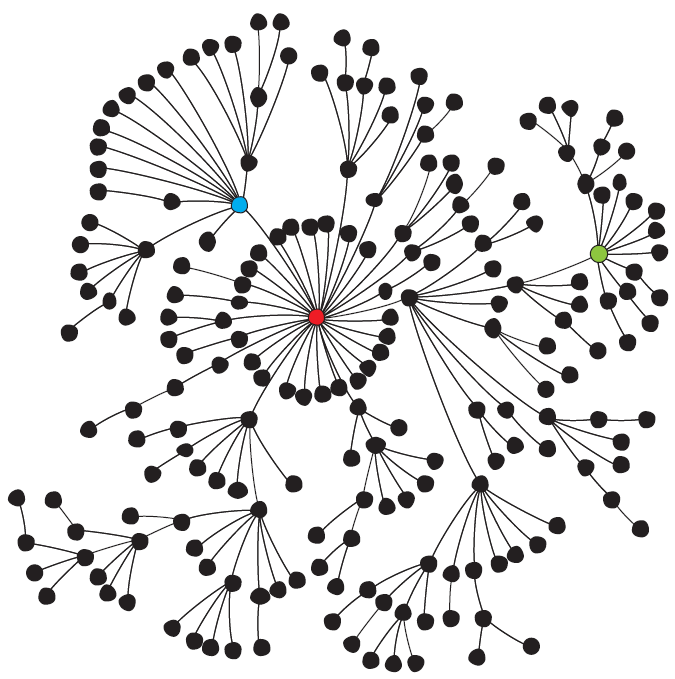
\includegraphics[width=0.4\textwidth]{images/scale-free-network.png}};

    \node (proc1) at (-3.5,2) [draw,thick,minimum width=2cm,minimum height=1cm,rounded corners=10pt] {Process 1};
    \node (proc2) at (-3.5,-2) [draw,thick,minimum width=2cm,minimum height=1cm,rounded corners=10pt] {Process $n$};

    \node (file1) at (0,2) [draw,thick,minimum width=2cm,minimum height=1cm,rounded corners=10pt] {GCV list 1};
    \node (file2) at (0,-2) [draw,thick,minimum width=2cm,minimum height=1cm,rounded corners=10pt] {GCV list $n$};
    
    \node (file_final) at (3,0) [draw,thick,minimum width=2cm,minimum height=1cm,rounded corners=10pt] {Final GCV list};
    
    \draw node[circle, minimum size=2cm, red, fill=red, fill opacity=0.2] (nodes1) at (-7.0,1.5)  {};
    \draw node[circle, minimum size=2cm, red, fill=green, fill opacity=0.2] (nodes2) at (-7.0,-1.5)  {};

    \draw[line width=2pt, loosely dotted] (-3.5,1) -- (-3.5,-1);
    \draw[line width=2pt, loosely dotted] (0,1) -- (0,-1);
    
%     \draw[red] (-12.0,9.5) rectangle (-1.0,9.0);
%     \draw[red] (-12.0,8.55) rectangle (-1.0,8.05);
    
    \draw[line,thick, ->] (nodes1) -- node[above] {chunk 1} (proc1) {};
    \draw[line,thick, ->] (nodes2) -- node[above] {chunk $n$} (proc2) {};
    \draw[line,thick, ->] (proc1) -- node[above] {GCVs} (file1) {};
    \draw[line,thick, ->] (proc2) -- node[above] {GCVs} (file2) {};
    \draw[line,thick, ->] (file1) -- (file_final.north west) {};
    \draw[line,thick, ->] (file2) -- (file_final.south west) {};

  \end{tikzpicture}
  \caption[Parallelisation process for the GCV computation]{Illustration of the parallelisation process for the GCV computation. For an input network, we split the nodes into different chunks and assign each chunk to a process. Each process computes the GCVs only for his chunk of nodes and writes them to an output file. At the end, all the GCV lists from the output files are assembled together into one final list. During the assembly process, the final GCV list is also sorted by node entry in order to easily visualise all the GCVs and to simplify our consistency checks.}
  \label{fig:parallelisation_process}
  \end{center}
\end{figure}%

%%%%%%%%%%%%%%%%%%%%%%%

\begin{figure}
\begin{lstlisting}
for each child process
{
  /* spawn a new process and store its PID */
  pids[proc_index] = fork();
  if (current process is a child)
  {
    /* open file suffixed by process number */
    FILE* out_file = fopen(out_name + proc_index, "w");
    /* find the nodes that the child needs to process */
    nodes_to_process = [CHUNK_SIZE * proc_index, CHUNK_SIZE * proc_index + 1]
    /* compute the GCV list and write them to the output */
    compute_gcv(input_graph, out_file, nodes_to_process);
    /* the child process closes the file and terminates */
    fclose(fp_out);
    return 0;
  }
}

/* Parent process waits on all children to finish execution */
for each child process
{
  waitpid(pids[proc_index]);
}
\end{lstlisting}
\caption[Pseudocode for the parallelisation logic]{Pseudocode for the parallelisation logic that is implemented in file \lstinline|e_gdv.cpp|. Note that the actual GCV computation takes place in the \lstinline|compute_gcv| function. The reason why the output file pointer is passed to this function is because we want each process to write the GCV signatures to the output files on the fly, as soon as they are computed. This helps us debug the software more easily and also avoid "out of memory" problems when processing large network files which have more than 11.000 nodes.}
\label{fig:pseudocode_parallelisation}
\end{figure}

Because of the way we chose to implement parallelisation, some processes tend to finish earlier than other. Even if every process computes the GCV for the same number of nodes in the network, computing the GCV for hub nodes takes considerably longer because they have large neighbouring subgraphs. As a result, some processes finish early while others get stuck with the GCV computation for some hub nodes. However, this limitation tends to become less obvious as the size of the input network increases. One way to overcome this problem is to redistribute the computation to the processes that finish early.

In order to evaluate the speedup from parallelisation, we repeatedly perform the GCV computation on the PPI, WTN and Metabolic networks using a variable number of processes and network size. Each experiment is also repeated 5 times and the average running time is reported. The machine we run the experiments is the \lstinline|Bionets02|, having the following specifications\footnote{The CPU type and memory size are taken from the output of the \lstinline|lshw| command. The specifications of the AMD Opteron 6282 SE processor are taken from the www.cpu-world.com website.}:
\begin{itemize}
 \item cpu: 4 x AMD Opteron(tm) Processor 6282 SE @ 2600MHz
 \begin{itemize}
  \item Number of cores: 16 
  \item Data width: 64 bit
  \item Level 1 cache size: 8 x 64 KB 2-way associative shared instruction caches, 16 x 16 KB 4-way associative data caches
  \item Level 2 cache size: 8 x 2 MB 16-way associative shared exclusive caches
 \end{itemize}
 \item memory: 125GB
\end{itemize}


We therefore calculate on \lstinline|Bionets02| the speedup obtained on the Human PPI, Human Metabolic and 2010 World Trade network as the number of processes increases from 1 to 64. The speedup $s_n$ when using $n$ processes is calculated as follows:
$$ s_n = 100\left(\frac{T_{1}}{T_{n}} - 1\right)$$\
where $T_{n}$ is the wall-clock time of execution when using $n$ processes, while $T_1$ is the wall-clock time of the serial execution. The final value is multiplied by 100 so that we can express it in percentage terms. Figure \ref{fig:time_threads} shows the speedup for the PPI, Metabolic and WTN networks. Each experiment has been run 5 times and the average running times $T_n$ have been used to compute the final speedup. When the number of processes is 2, we don't get any speedup in the execution, but as the number of processes increases, some speedup is clearly visible for the PPI and WTN networks. The Metabolic network only shows some speedup when 64 processes are running the computation. The PPI and the WTN networks also show a considerable speedup at the end, when executing the computation on 64 processes. It should be noted that the speedup of WTN becomes greater than the equivalent speedup of the PPI network when more than 32 processes are used.

\begin{figure}[H]
  \centering
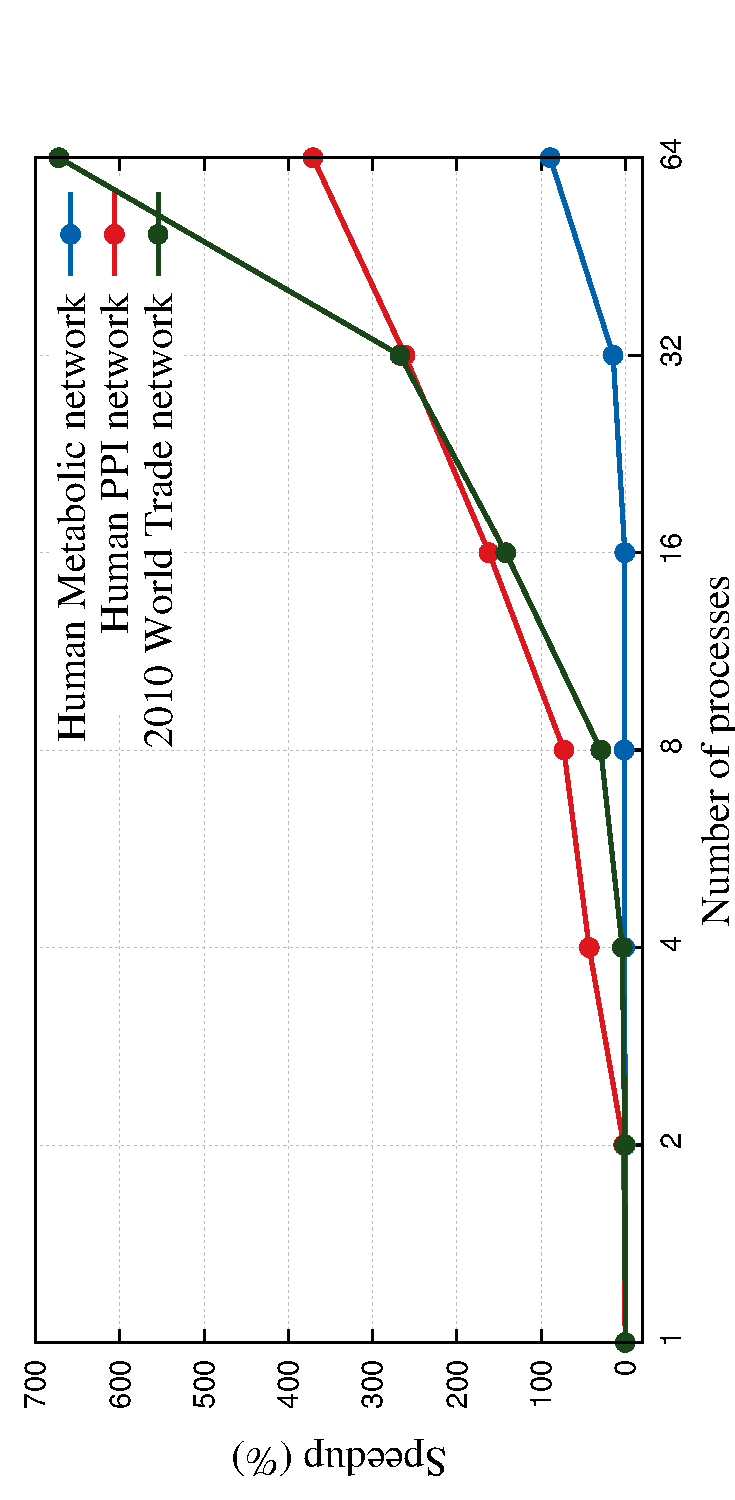
\includegraphics[angle=-90,scale=0.6]{../code/final_results/parallelisation_results/nr_processes2}
\caption[Parallelisation - speedup for PPI, Metabolic and 2010 WTN networks]{Speedup gained from parallelisation as the number of processes increases. The following three different networks have been tested: A human PPI network, a human metabolic network and a 2010 World Trade network (WTN). Although not immediately obvious from the graph because of the logarithmic $X$ axis, the speedup trend is linear in the number of processes. A maximum speedup of 680\% and 380\% is obtained for the WTN and the PPI network respectively when 64 processes are used.}
\label{fig:time_threads}
\end{figure}

After evaluating the speedup of the parallelisation, we are now interested to see how the execution time changes when we increase/decrease the problem size. In order to test for different problem sizes, we take a large network and randomly remove edges from it. We therefore generate networks that contain 50\%, 60\%, \dots , 100\% of the edges of the initial network. We then compute the execution time (wall-clock time) on each of these incomplete networks for a different number of processes. For each process and network size, 5 trials are run and the average execution time is reported. Figure \ref{fig:problem_size} shows the results obtained for this experiment. When the problem size is small, the execution time is fast regardless of the number of processes used. However, as the network size increases, the speedup gains from parallelisation become apparent, because the difference between lines widens. Eventually, when 64 processes are used, the execution time on the full network is approximately 32 seconds, 
which is 3-4 times faster than the equivalent execution time with 1 process. Note that the apparent inconsistencies between the PPI results in figure \ref{fig:time_threads} and the last column from figure \ref{fig:problem_size} might be because of the fact that the \lstinline|Bionets02| might have had other services from users running in the meantime that could have affected the performance.


\begin{figure}[H]
  \centering
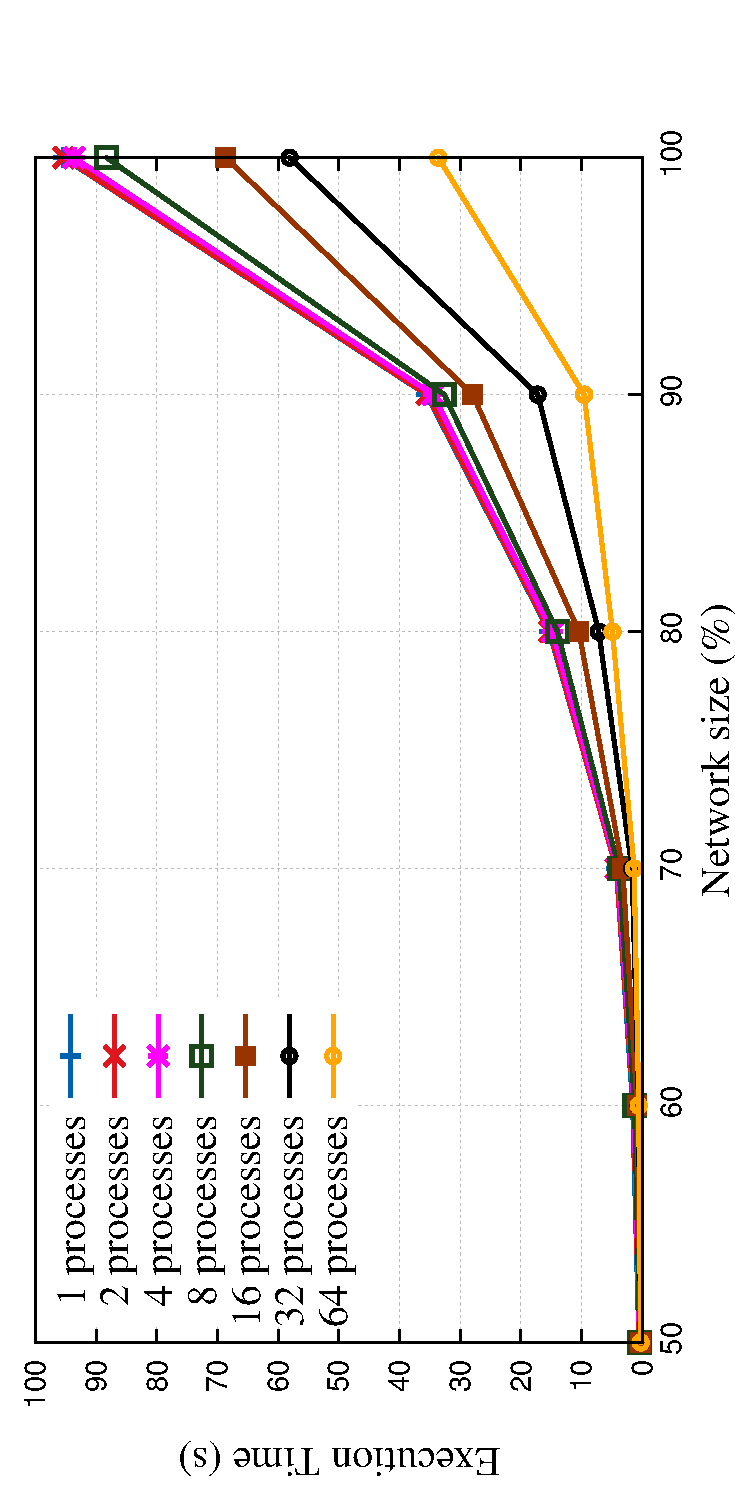
\includegraphics[angle=-90,scale=0.6]{../code/final_results/parallelisation_results/problem_size_human_ppi2}
\caption[Parallelisation - Execution time as the network size increases]{Execution time plotted for different number of processes as the network size increases. The input network used is the Human PPI network, and a network size of $p\%$ refers to the percentage of edges that were kept from the original network. For all network sizes, one can easily notice that the execution time gets faster as the number of processes increases. These results suggest that the gains in parallelisation are noticeable only for large networks.}
\label{fig:problem_size}
\end{figure}

The network that had the longest average runtime was the PPI network, with an execution time ranging from 95 seconds (1 process) to 32 seconds (64 processes). Although an execution time of 95 seconds is not problematic for our experiments, other PPI networks\footnote{the PPI networks from BioGRID - Full version, see section \ref{sec:cca_ppi_intro}} we have experimented with have taken around 10 hours to finish using 64 parallel processes. Moreover, other networks such as the literature network\footnote{We have also experimented with literature networks, which are networks of characters from a book. However, the results were not significant so we have not included them in this report.} of the Bible have taken several days to finish using 64 parallel processes. The reason the GCV computation takes so long to finish on these networks is because some processes get stuck with computing GCVs for hub nodes, which have very large neighbouring graphs.

In conclusion, parallelisation of GCV computation was a key part of the project that enabled us to run more experiments faster and to exploit all the computational resources of our machines. Some of the experiments on the PPI and literature networks would not have been possible without parallel computation.

\subsection{Pearsons's GCV correlation matrix}
\label{sec:metho_pears}

 In the background section \ref{pearsons_background}, we introduced the Pearson's GDV correlation matrix for a given graph. Similarly, the \emph{Pearson's GCV correlation matrix} can also be computed in order to find out which graphlets cluster together. This is important because graphlets that cluster together have a similar behaviour and also correlate with the same functional annotations. We present to the reader the steps used for computing the \emph{Pearson's GCV correlation matrix}, which uses the GCV (Graphlet Cluster Vector) instead of the GDV (Graphlet Degree Vector):
\begin{enumerate}
 \item We compute the Graphlet Cluster Vector (GCV) for every node in the
input network
 \item We then construct samples $ S_i, i\in {1,2,3, .. ,29} $
containing all the frequencies of the graphlet of type $i$ found in the GCVs of
the nodes. The length of $S_i$ would be equal to $N$, the number of nodes in the network.
 \item We compute the Pearson's correlation coefficient for each pair of samples $ (S_i, S_j) $ and we write them in the 29x29 correlation matrix $
C$ at position $(i,j)$.
\end{enumerate}

The program that computes the GCV correlation matrix has been written without using any library functions. Nevertheless, it took me a few of hours to identify some bugs and memory leaks. Using GDB and Valgrind has proven to be extremely helpful for this task. I also implemented my own function that computes the Pearson's coefficient for two samples $X$ and $Y$ and tested it using an excel spreadsheet that computed the correlation coefficient in parallel.

Unfortunately, the first heat maps that we get for the three main network classes (PPI, Metabolic and Trade) are not easy to interpret. See the initial image (top-left corner) from figure \ref{fig:heatmap_process}, which shows the original heat map obtained for the Human PPI network. Most of the graphlets display a high correlation (at least 0.5) and because of that we cannot distinguish clusters easily. Similar results are obtained for the other two networks: Human Metabolic and WTN. In order to identify which graphlets cluster together, we apply two main modifications to the matrices:
\begin{itemize}
 \item Normalisation: We normalise the correlation values so that they lie more evenly in the (0,1) range.
 \item Hierarchical clustering: In order to better identify clusters of graphlets that are highly correlated with each other, we perform hierarchical clustering on the set of 29 graphlet signatures.
\end{itemize}


\rowcolors{1}{blue1}{blue2}


%%%%%%%%%% GCV computation process %%%%%%%%%%%%%

\newcommand{\cellsizegcvtable}{1.45}

\newcommand{\gcvtable}{
\begin{tabular}{p{\cellsizegcvtable cm}p{\cellsizegcvtable cm}p{\cellsizegcvtable cm}p{\cellsizegcvtable cm}p{\cellsizegcvtable cm}p{0.5cm}}
 Graphlets    & GCV (node 1) & GCV (node 2) & GCV (node 3) & GCV (node 4) & \dots \\
 G1 & 2 & 3 & 6 & 9 & \dots \\ 
 G2 & 1 & 10 & 23 & 0 & \dots \\ 
 G3 & 0 & 3 & 5 & 14 & \dots \\ 
 G4 & 4 & 9 & 6 & 2 & \dots \\ 
 \dots &  \dots & \dots & \dots & \dots & \dots\\
 G29 & 1 & 14 & 6 & 0 & \dots \\  
\end{tabular}
}

\begin{figure}[h]
  \begin{center}
  \begin{tikzpicture}[scale=1.0,auto,swap,post/.style={->,shorten >=3pt,>=stealth',thick}]


    \node[inner sep=0pt] (1a) at (-9.0, 2.0) {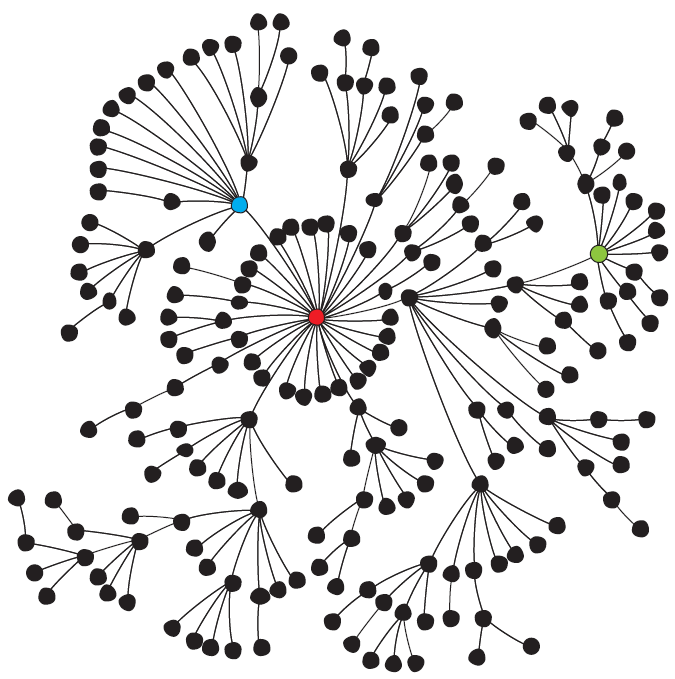
\includegraphics[width=0.4\textwidth]{images/scale-free-network.png}};
    \node[inner sep=0pt] (2a) at (-6.5, 9.0) {\gcvtable};
    \node[inner sep=0pt] (3a) at (-0.0, 2.0) {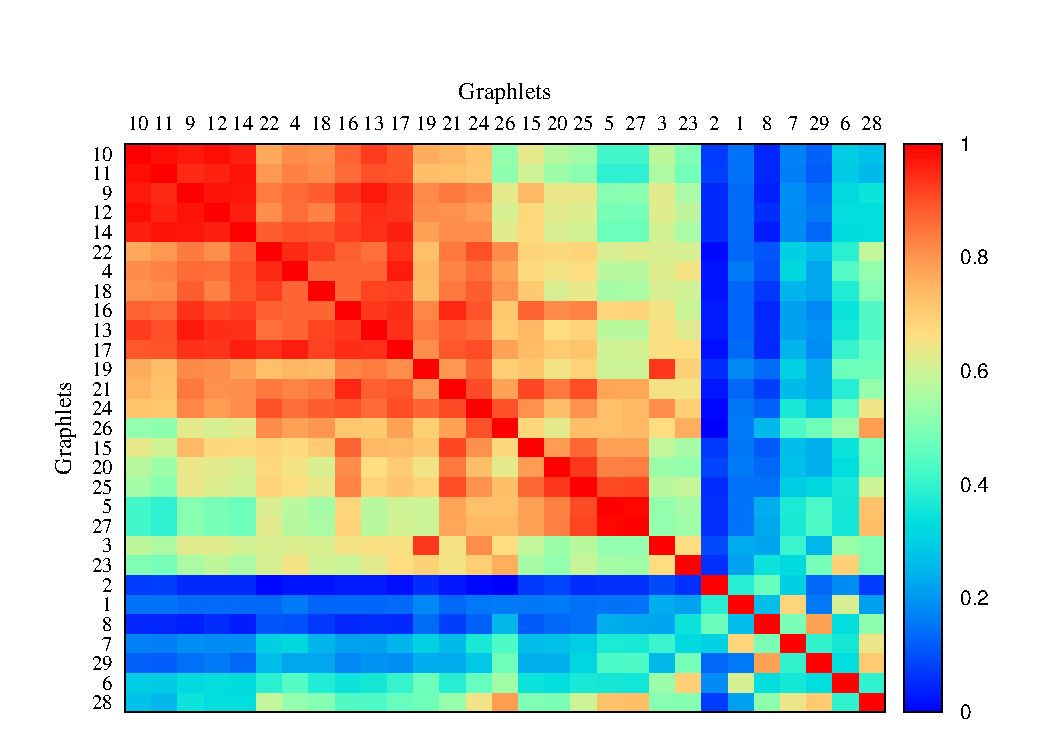
\includegraphics[scale=0.7]{../code/final_results_norm1/trade_2010_thresholded/heatmap_pearsons_hclust_trade_2010_thresholded2.pdf}};
    \node[text width=10em] (4a) at (2.5, 8.7) {$\rho(i,j) = $ Pearson's correlation between row vectors $i$ and $j$ };
    \node (5a) at (2.5, 1) {};
    \node (gcv_src) at (-1.0, 8.7) {};
    
    \draw[red] (-12.0,9.5) rectangle (-1.0,9.0);
    \draw[red] (-12.0,8.55) rectangle (-1.0,8.05);
	  
   \draw[post] (1a) -- node[right] {Graphlet Cluster Vectors (GCVs)} (1a |- 2a.south);
%     \path[hi, line width=1.0]  (4a)  -- (5a);
    \draw[post,rounded corners=5pt] (4a.south)-|(5a.north);
    \draw[post,rounded corners=5pt] (gcv_src) -- node[above] {} (gcv_src -| 4a.west) ;
    
  \end{tikzpicture}
  \caption[Computation process of the Pearson's GCV correlation matrix]{Computation process of the Pearson's GCV correlation matrix. For an input network, we compute a table of the GCV signatures for all the nodes in the input network. Afterwards, we compute the Pearson's correlation coefficient $\rho(i,j)$ between each pair of row vectors $i$ and $j$ and store it at position $M[i,j]$ in the correlation matrix $M$.}
  \label{fig:gcv_corr_process}
  \end{center}
\end{figure}%

%%%%%%%%%%%%%%%%%%%%%%%


% \begin{figure}[H]
%   \centering
%   \hbox{\hspace{-1cm}
%   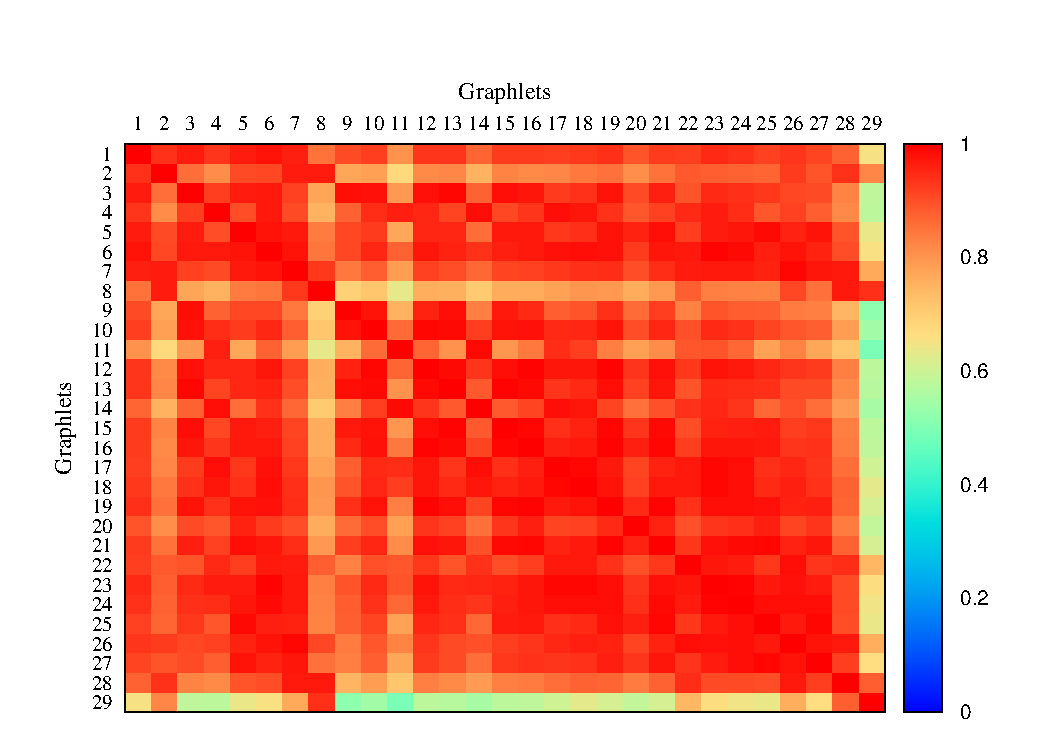
\includegraphics[scale=1.0]{../code/final_results/human_ppi/heatmap_pearsons_human_ppi2.pdf}}
%   \caption{Heatmap for the Pearson's GCV correlation matrix of the Human PPI network}
%   \label{ppi_heatmap}
% \end{figure}


\subsection{Normalisation}

Two main normalisation steps have been performed in order to spread out the correlation values over the (0,1) range:
\begin{enumerate}
 \item Feature scaling
 \item Polynomial scaling
\end{enumerate}

By feature scaling we denote a uniform scaling that makes the data fit on the (0,1) range. On the other hand, polynomial scaling applies a polynomial function to the input value. They are formally defined as follows:
\begin{mydef}
Let $X$ be a population and $min(X)$, $max(X)$ be the minimal respectively maximal value in $X$. Feature scaling is a transformation that converts each element $x \in X$ into an element $x'$ such that:
\begin{equation}
 x' = \frac{x - min(X)}{max(X) - min(X)}
\end{equation}
\end{mydef}


\begin{mydef}
Let $X$ be a population. Polynomial scaling is a transformation that converts each element $x \in X$ into an element $x'$ such that:
 $$x' = x^n$$ 
\end{mydef}



For each matrix, feature scaling is first applied followed by polynomial scaling. For both feature scaling and polynomial scaling, the set of all entries in the 2D matrix are used as the population vector $X$. After applying feature scaling, all the entries in the correlation matrix are converted to the (0,1) range. This results in both the input and output of the polynomial scaling to also be in the (0,1) range, regardless of the parameter $n$ that is used. 


\subsection{Hierarchical clustering}

Hierarchical clustering is a method that clusters data points according to how similar they are. In our case the data points were the 29 GCV correlation vectors, and the similarity measure used was given by the Euclidean distance. See section \ref{hier_clust} for background information on hierarchical clustering. The reason for clustering them is because we need to find out which graphlets are similar and which ones are different with each other. The graphlets that are similar probably have some common properties that we are able to identify and interpret.

We have used the python library \lstinline|Scipy| to run hierarchical clustering. We first calculate a distance matrix using the \lstinline|Scipy.spatial.distance|. This symmetric matrix stores the distances between every two data points as a 2D matrix. Afterwards, the hierarchical clustering is performed with the function call \lstinline|scipy.cluster.hierarchy.linkage(dist_matrix, method='complete')|. The method parameter refers to the type of hierarchical clustering that is performed. We have chosen to use Complete linkage\footnote{Complete linkage groups clusters together according to the shortest distance between the farthest points in the sets (see the definition for complete linkage in section \ref{hier_clust}).} because it avoids the so-called \emph{chaining phenomenon} of single linkage, where clusters are forced together due to outlier data points being close to each other, even though the majority of the data points might actually be away from each other. It has also been shown that complete 
linkage tends 
to create clusters of similar diameter \cite{everitt2001hierarchical}.

Each Pearson's correlation matrix is first normalised using both feature scaling and polynomial functions and then hierarchically clustered. We shall refer to this process as the \emph{Pearson's GCV correlation matrix life cycle}. More details about its implementation aspects can be found in section \ref{sec:life-cycle_framework}. Figure \ref{fig:heatmap_process} shows the \emph{Pearson's GCV correlation matrix life cycle} for the Human PPI network. One can clearly see that the initial matrix is very hard to interpret, having all correlations very high. On the other hand, the final matrix is very easy to interpret and clearly shows graphlet clusters formed along the diagonal. In this example, we used a a $4^{th}$ degree polynomial, but for other networks we found that other polynomial functions offer better results. Chapter \ref{chp:applications} presents the key results of the Pearson's matrices applied to different network classes.

%%%%%%%%%% Heatmap life cycle %%%%%%%%%%%%%

% Define the arm and angle options
\def\myarm{1cm}
\def\myangle{0}
\tikzset{
  arm/.default=1cm,
  arm/.code={\def\myarm{#1}}, % store value in \myarm
  angle/.default=0,
  angle/.code={\def\myangle{#1}} % store value in \myangle
}

% Define the myncbar to path
\tikzset{
    myncbar/.style = {to path={
        % We need to calculate a couple of coordinates to help us draw
        % the path. 
        let
            % Same as (\tikztotarget)++(\myangle:\myarm)
            \p1=($(\tikztotarget)+(\myangle:\myarm)$)
        in
            -- ++(\myangle:\myarm) coordinate (tmp)
            % Find the projection of the (tmp) coordinate
            % on the line from the target to p1
            --  node[below] {\hspace{1.0em}\begin{tabular}{c} $4^{th}$ degree polynomial scaling: \\ $x' = x^4$ \end{tabular}} ($(\tikztotarget)!(tmp)!(\p1)$)
            -- (\tikztotarget)\tikztonodes
    }}
}


\begin{figure}[h!]
  \rowcolors{1}{}{}
  \hspace{-3.0em}
  \begin{tikzpicture}[scale=1.0,auto,swap,post/.style={->,shorten >=3pt,>=stealth',thick}]

    \node[inner sep=0pt] (orig) at (0.0, 8.0) {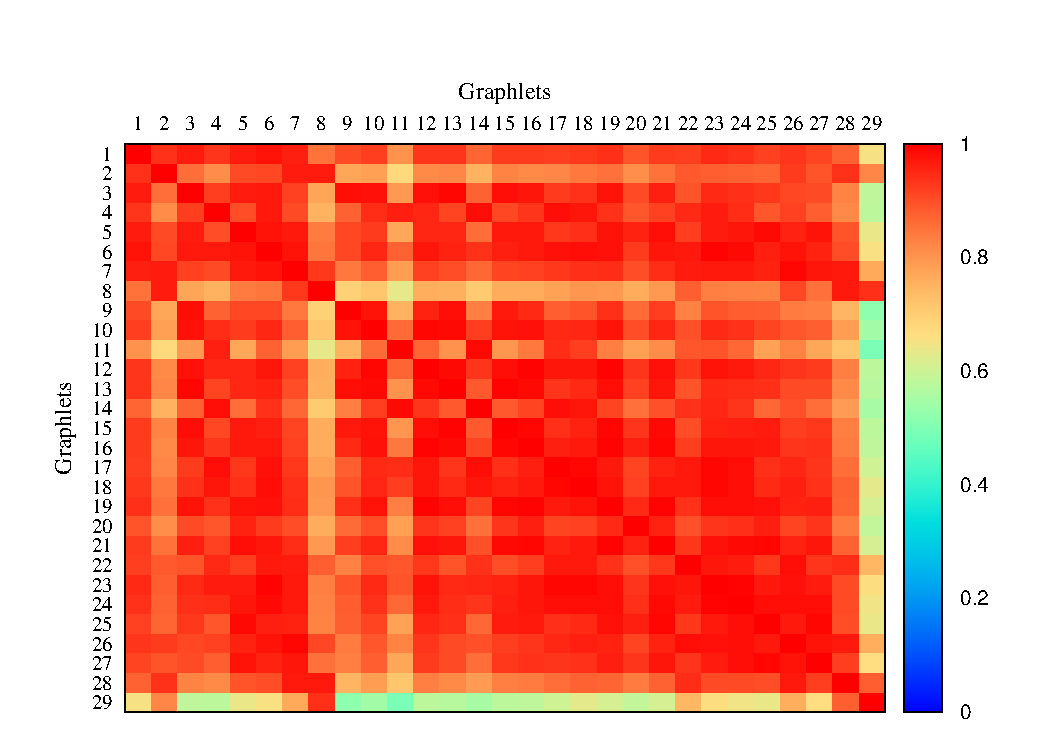
\includegraphics[scale=0.5]{../code/final_results/human_ppi/heatmap_pearsons_human_ppi2.pdf}};
    \node at (orig.north) {\textbf{Initial matrix}};
    \node[inner sep=0pt] (feature_scaled) at (0.0, 0.0) {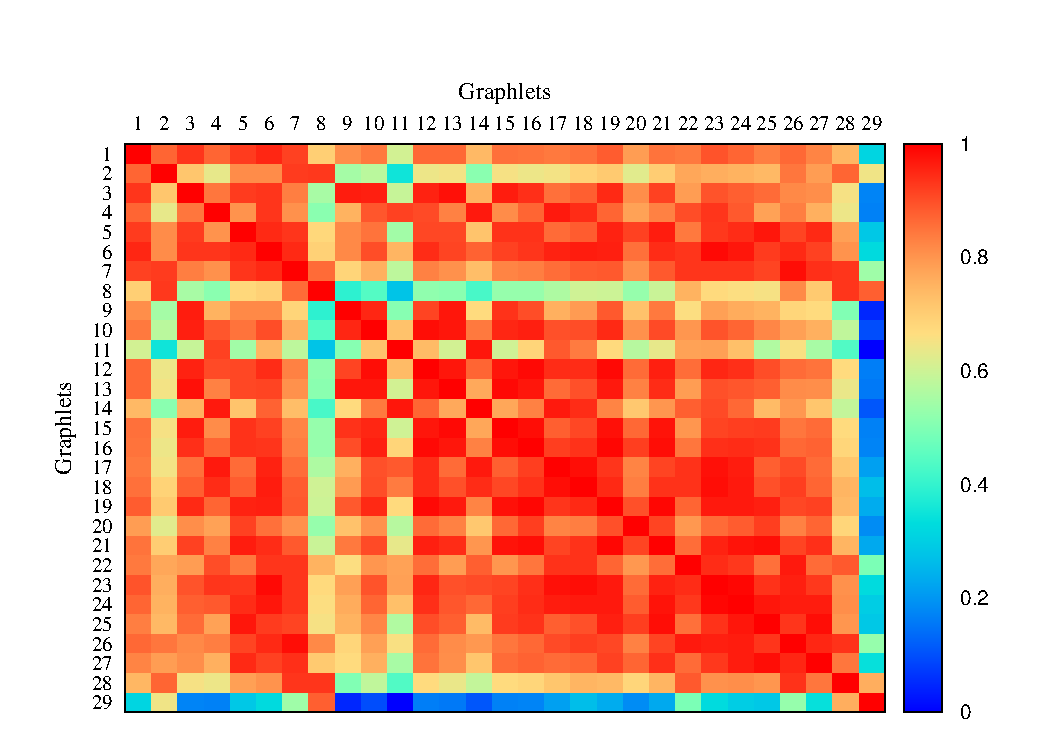
\includegraphics[scale=0.5]{../code/final_results/human_ppi/heatmap_pearsons_normalized_human_ppi2.pdf}};
    \node[inner sep=0pt] (poly4) at (9.0, 0.0) {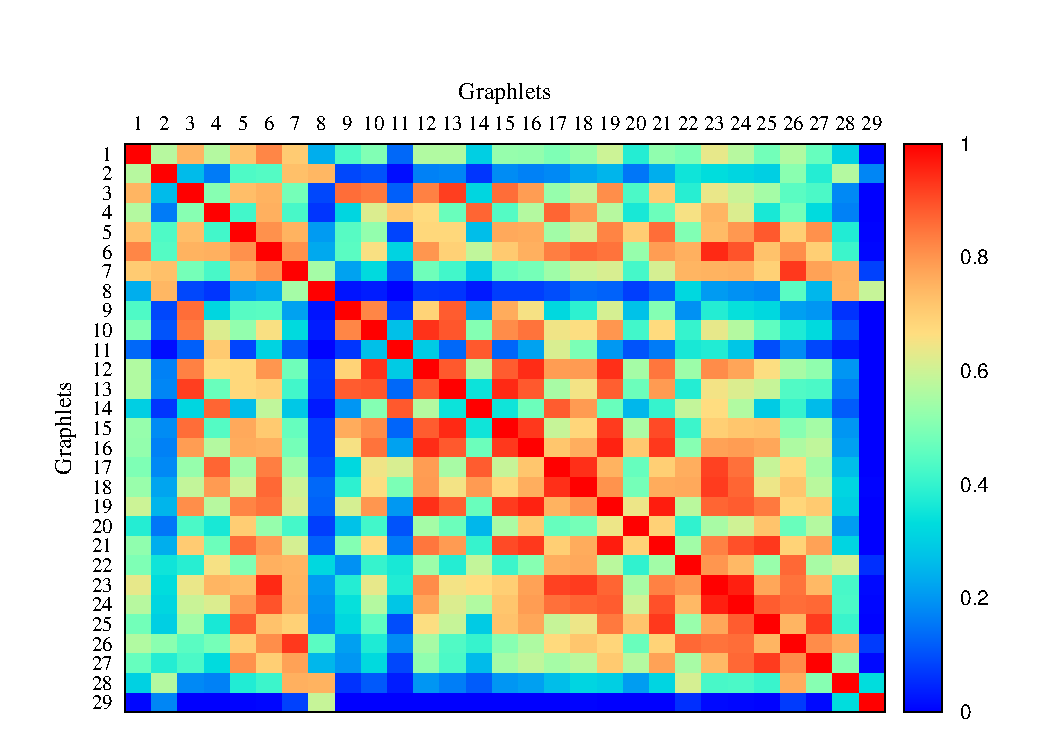
\includegraphics[scale=0.5]{../code/final_results/human_ppi/heatmap_pearsons_normalized_human_ppi-poly-42.pdf}};
    \node[inner sep=0pt] (hclust) at (9.0, 8.0) {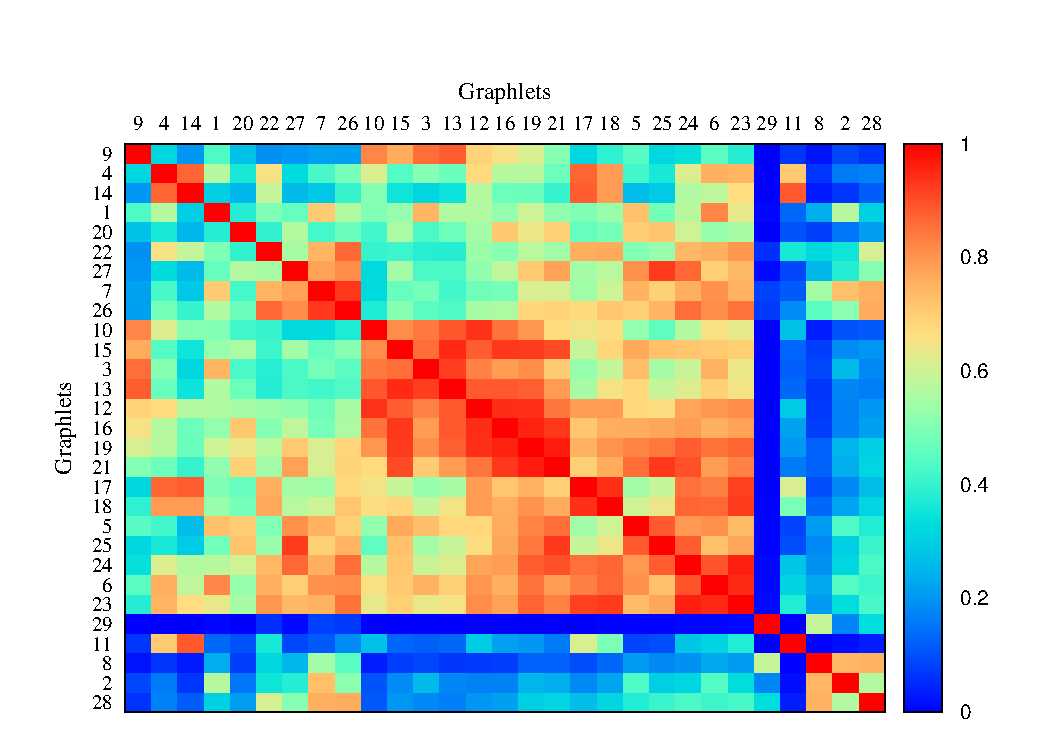
\includegraphics[scale=0.5]{../code/final_results/human_ppi/heatmap_pearsons_hclust_human_ppi-poly-42.pdf}};
    \node at (hclust.north) {\textbf{Final matrix}};
    
    \draw[line,thick, ->] (orig) -- node[right] {\begin{tabular}{l} feature scaling: \\ $x' = \frac{x - min}{max - min}$ \end{tabular}} (feature_scaled) {};
    \draw [->,thick] (feature_scaled.south)  to[myncbar,arm=-0.5cm,angle=90]  (poly4.south);
    \draw[line,thick, ->] (poly4) -- node[right] {\begin{tabular}{l}hierarchical clustering\\(complete linkage)\end{tabular}} (hclust) {};


  \end{tikzpicture}
  \caption[Pearson's GCV correlation matrix life cycle for the Human PPI network]{Pearson's GCV correlation matrix life cycle for the Human PPI network. The initial Pearson's GCV correlation matrix is on the top-left corner and the final matrix is on the top-right corner, after feature scaling, polynomial scaling and hierarchical clustering operations are applied. One can see that in the final matrix graphlet clusters are distinguished more easily compared to the initial matrix. The operation order is anti-clockwise. When feature scaling, the range of the correlations $[min, max]$ is scaled to $[0,1]$. After performing polynomial scaling using a $4^{th}$ degree function, the correlations are lowered even more. Finally, after applying hierarchical clustering, similar graphlets cluster together along the diagonal. Hierarchical clustering uses complete linkage for grouping GCVs and the Euclidean distance to compute the difference between GCVs.}
  \label{fig:heatmap_process}
\end{figure}%

%%%%%%%%%%%%%%%%%%%%%%%

\subsection{Canonical Correlation Analysis}

Graphlets only give us information about the topology of the network connections. However, in order to associate them with node functions or annotations, we need to correlate the GCV with a vector of node annotations. Canonical Correlation Analysis (CCA) is able to do exactly this and also give us a p-value, that can quantify the significance of the result. The theory behind CCA is given in background section \ref{cca_background}. In this section, we present how we applied CCA in our experiments and discuss implementation details.

% Discuss about Darren's scripts, how I modified them
Initially, I experimented with CCA using three different implementations:
\begin{itemize}
 \item \lstinline|Python Scikit|: a Python implementation that is based on algorithms by Jacob A. Wegelin \cite{wegelin2000survey}. The problem with this implementation is the poor documentation available.
 \item \lstinline|Matlab|: based on two books by Krzanowski, W. J. \cite{krzanowski2000principles} and Seber, G. A \cite{seber2009multivariate}. The documentation is good, but the implementation does not provide canonical cross-loadings.
 \item Darren Davis's \lstinline|R| script: Darren Davis is a collaborator of N. Pr\v{z}ulj who has previously applied CCA on GDV signatures. His \lstinline|R| implementation also performs some preprocessing of the data points and covariance matrices, such as scaling, centring\footnote{The data points are centred around the origin} and regularisation\footnote{If the covariance matrix is singular, a weighted identity matrix is added to it. More formally, if the covariance matrix of the data points is $S$, then $S' = S + \lambda I$}. This implementation is also accompanied by some python scripts that can preprocess all the trade networks for a given range of years.
\end{itemize}

We have decided to use Darren Davis's script, mainly because it is able to calculate cross-loadings and it also had 5 accompanying python scripts that preprocess the economic networks. Therefore, we refactored the \lstinline|R| script in order to allow several parameters to be passed from the command line. On the other hand, the preprocessing python scripts have been extensively modified to deal with the new GCV signature and for enabling them to process different annotation files, such as EC numbers (see section \ref{metabolic_annotations}) or Boone's and von Mering's annotations (see section \ref{ppi_annotations}).

\hilight{Discuss about how I converted the annotation files}

% Add reference with example pictures and tables once they have been added.

Darren Davis's \lstinline|R| script gives us all the canonical correlation eigenvectors, with their associated correlation and p-values and writes them to a text file. The eigenvectors are sorted in descending order by their correlation strength, so the first eigenvector is the most significant. We therefore created a parser for this file that finds the first eigenvector and produces a \LaTeX\ table with all the cross-loadings and the respective overall correlation and p-value. This script has been used for generating all the CCA tables in this report. We have also created another script that creates a vector graphics image containing the following:
\begin{itemize}
 \item an indicator list on the left-hand side where is element is coloured from green (1) to red (-1) according to their canonical cross-loading.
 \item a top-right panel containing the graphlets with the highest canonical cross-loading.
 \item a bottom-right panel containing the graphlets with the lowest canonical cross-loading.
 \item a gradient bar in the middle measuring correlation where the graphlets and indicators are connected.
\end{itemize}

This script is written in Python and generates fragments of \lstinline|Tikz| code that can be used by \LaTeX to generate the image. In order to get the images in their final state, further manual modifications are performed. The images are very intuitive to understand and will be used extensively during the presentation. They are also included in this report in figures \ref{fig:all_trade_cca_unnorm_black}, \ref{fig:all_trade_cca_black} and \ref{fig:ppi_cca_black}. However, we don't include them for all CCA results in the report because they don't give the exact correlations which are required for a careful analysis.

\subsection{Network life cycle framework}
\label{sec:life-cycle_framework}
In order to be able to run all our experiments in an automatic fashion and for a variety of networks, we implemented a few \emph{network life cycle frameworks} that take a network and run all the statistical experiments automatically. The frameworks are defined by commands in a Makefile that chain a variety of scripts. We wrote two main classes of such frameworks: 
\begin{enumerate}
 \item Pearson's GCV Correlation matrix life cycle: used for computing all the correlation matrices and generating several types of heat maps.
 \item Canonical Correlation life cycle: used for preprocessing a network and its annotation file and applying CCA on them.
\end{enumerate}

Both of these are described in more detail in the following subsections.

\subsubsection{Pearson's GCV correlation matrix life cycle}

The \emph{Pearson's GCV correlation matrix life cycle} takes an input network and computes several GCV correlation matrices and their corresponding heat maps. Several environment variables need to be set in order to run it, such as the network source folder, network file, generated folder\footnote{The generated folder is used for storing all the program results} and the GCV normalisation type\footnote{A binary value that decides whether the GCV is normalised or not.}. The steps that are performed in the life cycle are as follows:
\begin{enumerate}
 \item Initial file handling: Several directories are created and input files are copied over.
 \item GCV computation using \lstinline|e_gdv.cpp|\footnote{The name of the script is derived from "extended gdv", because at the time we started writing the script we were not decided on the name for the new signature.}
 \item Average network GCV computation
 \item Computation of the Pearson's GCV correlation matrix
 \item Computation of 4 types of normalised correlation matrices\footnote{The matrices are normalised with first, second, third and fourth degree polynomials. The higher the degree, the stronger the contrast between correlation values will become.}
 \item Hierarchical clustering on all the correlation matrices
 \item Heat map generation of all the correlation matrices using \lstinline|gnuplot|
\end{enumerate}


\subsubsection{Canonical Correlation Analysis life cycle}

A different framework was set up for Canonical Correlation Analysis. In order to run CCA on an input network, several preprocessing steps are required that transform the GCV and annotation files. For the World Trade network, the steps performed by the CCA life cycle are defined below:
\begin{enumerate}
 \item Initial file handling: the output folders are created and input files are copied over.
 \item Conversion of the GCV dump file to a CSV file for each of the 48 networks over the period 1962-2010.
 \item Aggregation of the above per-year GCV CSV files into a single GCV file.
 \item Aggregation of the economic indicator files into a single CSV file. Country/year entries with incomplete data are dropped.
 \item Augmentation of the basic economic indicators with composed economic indicators (e.g. GDP per capita x Population to get the total GDP of a country).
 \item Alignment of the GCV entries with the final economic indicators.
 \item execution of the actual Canonical Correlation Analysis
\end{enumerate}

\hilight{add the python files for each of these steps. the listing env has some probs with wrapping though}

The CCA life cycle described above is specific for the Trade networks. Similar frameworks were created for the other networks, which use different types of annotations. The steps performed are similar, but they use different parameters and one different preprocessing script that converts the indicators to a CSV file. It must be noted that the Python scripts performing the above steps are based on scripts created by Darren Davis for the GDV-based CCA.

\subsection{Unit testing}

Throughout the project we implemented a small suite of unit tests that checks the basic functionality of the GCV signature computation. We used the \lstinline|BOOST| unit testing framework written in \verb!C++! because of the following reasons:
\begin{itemize}
 \item The core algorithm that computes the GCV signature has also been written in \verb!C++!, which made integration easy.
 \item The \lstinline|BOOST| testing framework has very useful features such as:
 \begin{itemize}
  \item Grouping test cases into suites.
  \item The ability of running multiple, independent tests in parallel.
  \item The possibility of seeing the progress of long and complex tests.
 \end{itemize}
 \item There exists a variety of online tutorials and learning materials on the \lstinline|BOOST| testing framework
\end{itemize}

We wrote unit tests that check for the correctness of the GCV signature on PPI, Metabolic and World Trade networks. Moreover, we also tested the GCV on a small number of toy networks and compared the results with GCV signatures that were calculated by hand. Furthermore, we also tested the parallel computation in the following manner:
\begin{enumerate}
 \item For a given input network, we compute the GCV signature list several times, using an increasing number of processes.
 \item We compare each of the generated GCV lists for consistency. 
\end{enumerate}

This parallelisation test actually helped us discover a bug in the code caused by a null pointer exception, which only occured when 2 or more processes were used. This only affected a few of the processes that accessed the illegal area of the virtual memory and stopped their execution. As a result, the resulting GCV dump was incomplete, and this aspect was not immediately obvious without a close examination of the GCV list. 

The unit tests in our suite can be run using the Makefile command: \lstinline|make test|. This will execute all the tests in the test suite. One can also run individual tests or a subset of all the tests in the suite. Running two tests on the WTN network using 16 and 32 processes for the GCV computation produces an output similar to the one in figure \ref{fig:unit_test_output}.

\definecolor{test_green}{HTML}{003300} % 
\definecolor{test_blue}{HTML}{0033CC} % 

\lstdefinestyle{base}{
  language=C,
  emptylines=1,
  breaklines=true,
  basicstyle=\ttfamily\color{black},
  moredelim=**[is][\color{test_green}\textbf{}]{@}{@},
}

\begin{figure}[H]
\begin{lstlisting}[style=base,escapechar=!]
!\textcolor{test_blue}{Running 2 test cases...}!

!\textcolor{test_blue}{Running:}! ./e_gdv trade_2010_thresholded.gw test_bank/trade_2010_thresholded 16
Finished parsing the LEDA file
Waiting on the children ...Children have finished processing. Assembling the files...Running: cat test_bank/trade_2010_thresholded.0* > test_bank/trade_2010_thresholded.ndump2;rm test_bank/trade_2010_thresholded.0*

@Test successful@

!\textcolor{test_blue}{Running:}! ./e_gdv trade_2010_thresholded.gw test_bank/trade_2010_thresholded 32
Finished parsing the LEDA file
Waiting on the children ...Children have finished processing. Assembling the files...Running: cat test_bank/trade_2010_thresholded.0* > test_bank/trade_2010_thresholded.ndump2;rm test_bank/trade_2010_thresholded.0*
% 
@Test successful@


@*** No errors detected@

\end{lstlisting}
\caption[Command-line output when running two unit tests on the 2010 World Trade network]{Command-line output when running two unit tests on the 2010 World Trade network using 16 and 32 processes. For each test, the input network LEDA file is first parsed and then the parent waits until all children finish their processing. When the children processes finish their work, their output files are assembled together and checked for consistency.}
\label{fig:unit_test_output}
\end{figure}


% Chapter 4
\chapter{Applications}
\label{chp:applications}
%You are free to write up any additional material that will appear in the final
%report, for example a section or chapter describing a significant component of
%the design/implementation that you have already completed.  Avoid any
%additional material that is not re-usable in the final report.

\newcommand{\gscaling}{0.7}

\newcommand{\gone}{
    \begin{tabular}{>{\centering\bfseries}m{1in} >{\centering}m{0in}}	
      \begin{tikzpicture}[scale=\gscaling,auto,swap]

	% define the round nodes
	\foreach \pos/\name/\label in {
	  {(0,1)//1a},
	  {(0,0)//2a},
	  {(0,-1)//3a}}
	  \node[vertex2] (\label) at \pos {$\name$} ;

	%neighbouring graph
	      
	\path[hi, line width=1.0]  (1a)  -- (2a);
	\path[hi, line width=1.0]  (2a)  -- (3a);

	
      \end{tikzpicture} & \Large{$G_{1}$}
    \end{tabular}
}

\newcommand{\gonecca}[1]{
    \begin{tabular}{>{\centering\bfseries}m{0.4in} >{\centering}m{0in}}	
      \begin{tikzpicture}[scale=\gscaling,auto,swap]

	% define the round nodes
	\foreach \pos/\name/\label in {
	  {(0,1)//1a},
	  {(0,0)//2a},
	  {(0,-1)//3a}}
	  \node[vertex2,draw=#1,fill=#1] (\label) at \pos {$\name$} ;

	%neighbouring graph
	      
	\path[hi, line width=1.0,draw=#1]  (1a)  -- (2a);
	\path[hi, line width=1.0,draw=#1]  (2a)  -- (3a);

	
      \end{tikzpicture} \cellcolor{black} & \cellcolor{black}\textcolor{white}{\Large{$G_{1}$}}
    \end{tabular}
}

\newcommand{\gtwo}{
    \begin{tabular}{>{\centering\bfseries}m{1in} >{\centering}m{0in}}	
      \begin{tikzpicture}[scale=\gscaling * 1.3,auto,swap]

	% define the round nodes
	\foreach \pos/\name/\label in {
	  {(0,1.3)//1a},
	  {(-0.7,0)//2a},
	  {(0.7,0)//3a}}
	  \node[vertex2] (\label) at \pos {$\name$} ;

	%neighbouring graph
	      
	\path[hi, line width=1.0]  (1a)  -- (2a);
	\path[hi, line width=1.0]  (2a)  -- (3a);
	\path[hi, line width=1.0]  (3a)  -- (1a);

	
      \end{tikzpicture} & \Large{$G_{2}$}
    \end{tabular}
}


\newcommand{\gtwocca}[1]{
    \begin{tabular}{>{\centering\bfseries}m{0.7in} >{\centering}m{0in}}	
      \begin{tikzpicture}[scale=\gscaling * 1.3,auto,swap]

	% define the round nodes
	\foreach \pos/\name/\label in {
	  {(0,1.3)//1a},
	  {(-0.7,0)//2a},
	  {(0.7,0)//3a}}
	  \node[vertex3,draw=#1,fill=#1] (\label) at \pos {$\name$} ;

	%neighbouring graph
	      
	\path[hi, line width=1.0,draw=#1]  (1a)  -- (2a);
	\path[hi, line width=1.0,draw=#1]  (2a)  -- (3a);
	\path[hi, line width=1.0,draw=#1]  (3a)  -- (1a);

	
      \end{tikzpicture} \cellcolor{black} & \cellcolor{black}\textcolor{white}{\Large{$G_{2}$}}
    \end{tabular}
}

\newcommand{\gfive}{
    \begin{tabular}{>{\centering\bfseries}m{1in} >{\centering}m{0in}}	
      \begin{tikzpicture}[scale=\gscaling * 1.5,auto,swap]

	% define the round nodes
	\foreach \pos/\name/\label in {
	  {(0,0)//1a},
	  {(0,1)//2a},
	  {(1,1)//3a},
	  {(1,0)//4a}}
	  \node[vertex2] (\label) at \pos {$\name$} ;

	%neighbouring graph
	      
	\path[hi, line width=1.0]  (1a)  -- (2a);
	\path[hi, line width=1.0]  (2a)  -- (3a);
	\path[hi, line width=1.0]  (3a)  -- (4a);
	\path[hi, line width=1.0]  (1a)  -- (4a);


	
      \end{tikzpicture} & \Large{$G_{5}$}
    \end{tabular}
}

\newcommand{\gsix}{
    \begin{tabular}{>{\centering\bfseries}m{1in} >{\centering}m{0in}}	
      \begin{tikzpicture}[scale=\gscaling,auto,swap]

	% define the round nodes
	\foreach \pos/\name/\label in {
	  {(0,0)//1a},
	  {(-0.8,1)//2a},
	  {(0.8,1)//3a},
	  {(0,-1)//4a}}
	  \node[vertex2] (\label) at \pos {$\name$} ;

	%neighbouring graph
	      
	\path[hi, line width=1.0]  (1a)  -- (2a);
	\path[hi, line width=1.0]  (2a)  -- (3a);
	\path[hi, line width=1.0]  (1a)  -- (3a);
	\path[hi, line width=1.0]  (1a)  -- (4a);


	
      \end{tikzpicture} & \Large{$G_{6}$}
    \end{tabular}
}


\newcommand{\gsixcca}[1]{
    \begin{tabular}{>{\centering\bfseries}m{0.7in} >{\centering}m{0in}}	
      \begin{tikzpicture}[scale=\gscaling,auto,swap]

	% define the round nodes
	\foreach \pos/\name/\label in {
	  {(0,0)//1a},
	  {(-0.8,1)//2a},
	  {(0.8,1)//3a},
	  {(0,-1)//4a}}
	  \node[vertex2,draw=#1,fill=#1] (\label) at \pos {$\name$} ;

	%neighbouring graph
	      
	\path[hi, line width=1.0,draw=#1]  (1a)  -- (2a);
	\path[hi, line width=1.0,draw=#1]  (2a)  -- (3a);
	\path[hi, line width=1.0,draw=#1]  (1a)  -- (3a);
	\path[hi, line width=1.0,draw=#1]  (1a)  -- (4a);


	
      \end{tikzpicture} \cellcolor{black} & \cellcolor{black}\textcolor{white}{\Large{$G_{6}$}}
    \end{tabular}
}

\newcommand{\gseven}{
    \begin{tabular}{>{\centering\bfseries}m{1in} >{\centering}m{0in}}	
      \begin{tikzpicture}[scale=\gscaling * 1.2,auto,swap]

	% define the round nodes
	\foreach \pos/\name/\label in {
	  {(-1.0,0)//1a},
	  {(1,0)//2a},
	  {(0,1)//3a},
	  {(0,-1)//4a}}
	  \node[vertex2] (\label) at \pos {$\name$} ;

	%neighbouring graph
	      
	\path[hi, line width=1.0]  (1a)  -- (3a);
	\path[hi, line width=1.0]  (1a)  -- (4a);
	\path[hi, line width=1.0]  (2a)  -- (3a);
	\path[hi, line width=1.0]  (2a)  -- (4a);
	\path[hi, line width=1.0]  (3a)  -- (4a);

	
      \end{tikzpicture} & \Large{$G_{7}$}
    \end{tabular}
}


\newcommand{\geight}{
    \begin{tabular}{>{\centering\bfseries}m{1in} >{\centering}m{0in}}	
      \begin{tikzpicture}[scale=\gscaling * 1.3,auto,swap]

	% define the round nodes
	\foreach \pos/\name/\label in {
	  {(0,0)//1a},
	  {(-0.7,-0.6)//2a},
	  {(0.7,-0.6)//3a},
	  {(0,1)//4a}}
	  \node[vertex2] (\label) at \pos {$\name$} ;

	%neighbouring graph
	      
	\path[hi, line width=1.0]  (1a)  -- (2a);
	\path[hi, line width=1.0]  (1a)  -- (3a);
	\path[hi, line width=1.0]  (1a)  -- (4a);
	\path[hi, line width=1.0]  (2a)  -- (3a);
	\path[hi, line width=1.0]  (2a)  -- (4a);
	\path[hi, line width=1.0]  (3a)  -- (4a);

	
      \end{tikzpicture} & \Large{$G_{8}$}
    \end{tabular}
}



\newcommand{\geightcca}[1]{
    \begin{tabular}{>{\centering\bfseries}m{0.7in} >{\centering}m{0in}}	
      \begin{tikzpicture}[scale=\gscaling * 1.3,auto,swap]

	% define the round nodes
	\foreach \pos/\name/\label in {
	  {(0,0)//1a},
	  {(-0.7,-0.6)//2a},
	  {(0.7,-0.6)//3a},
	  {(0,1)//4a}}
	  \node[vertex3,draw=#1,fill=#1] (\label) at \pos {$\name$} ;

	%neighbouring graph
	      
	\path[hi, line width=1.0,draw=#1]  (1a)  -- (2a);
	\path[hi, line width=1.0,draw=#1]  (1a)  -- (3a);
	\path[hi, line width=1.0,draw=#1]  (1a)  -- (4a);
	\path[hi, line width=1.0,draw=#1]  (2a)  -- (3a);
	\path[hi, line width=1.0,draw=#1]  (2a)  -- (4a);
	\path[hi, line width=1.0,draw=#1]  (3a)  -- (4a);

	
      \end{tikzpicture} \cellcolor{black} & \cellcolor{black}\textcolor{white}{\Large{$G_{8}$}}
    \end{tabular}
}

\newcommand{\gnine}{
    \begin{tabular}{>{\centering\bfseries}m{1in} >{\centering}m{0in}}	
      \begin{tikzpicture}[scale=\gscaling,auto,swap]

	% define the round nodes
	\foreach \pos/\name/\label in {
	  {(0,2)//1a},
	  {(0,1)//2a},
	  {(0,0)//3a},
	  {(0,-1)//4a},
	  {(0,-2)//5a}}
	  \node[vertex2] (\label) at \pos {$\name$} ;

	%neighbouring graph
	      
	\path[hi, line width=1.0]  (1a)  -- (2a);
	\path[hi, line width=1.0]  (2a)  -- (3a);
	\path[hi, line width=1.0]  (3a)  -- (4a);
	\path[hi, line width=1.0]  (4a)  -- (5a);


	
      \end{tikzpicture} & \Large{$G_{9}$}
    \end{tabular}
}

\newcommand{\gninecca}[1]{
    \begin{tabular}{>{\centering\bfseries}m{0.7in} >{\centering}m{0in}}	
      \begin{tikzpicture}[scale=\gscaling,auto,swap]

	% define the round nodes
	\foreach \pos/\name/\label in {
	  {(0,2)//1a},
	  {(0,1)//2a},
	  {(0,0)//3a},
	  {(0,-1)//4a},
	  {(0,-2)//5a}}
	  \node[vertex3,draw=#1,fill=#1] (\label) at \pos {$\name$} ;

	%neighbouring graph
	      
	\path[hi, line width=1.0,draw=#1]  (1a)  -- (2a);
	\path[hi, line width=1.0,draw=#1]  (2a)  -- (3a);
	\path[hi, line width=1.0,draw=#1]  (3a)  -- (4a);
	\path[hi, line width=1.0,draw=#1]  (4a)  -- (5a);


	
      \end{tikzpicture} \cellcolor{black} & \cellcolor{black}\textcolor{white}{\Large{$G_{9}$}}
    \end{tabular}
}


\newcommand{\gten}{
    \begin{tabular}{>{\centering\bfseries}m{1in} >{\centering}m{0in}}	
      \begin{tikzpicture}[scale=\gscaling,auto,swap]

	% define the round nodes
	\foreach \pos/\name/\label in {
	  {(0,2)//1a},
	  {(0,1)//2a},
	  {(0,0)//3a},
	  {(-0.7,-0.7)//4a},
	  {(0.7,-0.7)//5a}}
	  \node[vertex2] (\label) at \pos {$\name$} ;

	%neighbouring graph
	      
	\path[hi, line width=1.0]  (1a)  -- (2a);
	\path[hi, line width=1.0]  (2a)  -- (3a);
	\path[hi, line width=1.0]  (3a)  -- (4a);
	\path[hi, line width=1.0]  (3a)  -- (5a);


	
      \end{tikzpicture} & \Large{$G_{10}$}
    \end{tabular}
}



\newcommand{\gtencca}[1]{
    \begin{tabular}{>{\centering\bfseries}m{0.7in} >{\centering}m{0in}}	
      \begin{tikzpicture}[scale=\gscaling,auto,swap]

	% define the round nodes
	\foreach \pos/\name/\label in {
	  {(0,2)//1a},
	  {(0,1)//2a},
	  {(0,0)//3a},
	  {(-0.7,-0.7)//4a},
	  {(0.7,-0.7)//5a}}
	  \node[vertex3,draw=#1,fill=#1] (\label) at \pos {$\name$} ;

	%neighbouring graph
	      
	\path[hi, line width=1.0,draw=#1]  (1a)  -- (2a);
	\path[hi, line width=1.0,draw=#1]  (2a)  -- (3a);
	\path[hi, line width=1.0,draw=#1]  (3a)  -- (4a);
	\path[hi, line width=1.0,draw=#1]  (3a)  -- (5a);


	
      \end{tikzpicture} \cellcolor{black} & \cellcolor{black}\textcolor{white}{\Large{$G_{10}$}}
    \end{tabular}
}

\newcommand{\geleven}{
    \begin{tabular}{>{\centering\bfseries}m{1in} >{\centering}m{0in}}	
      \begin{tikzpicture}[scale=\gscaling,auto,swap]

	% define the round nodes
	\foreach \pos/\name/\label in {
	  {(0,0)//1a},
	  {(0,1)//2a},
	  {(-1,0)//3a},
	  {(0,-1)//4a},
	  {(1,0)//5a}}
	  \node[vertex2] (\label) at \pos {$\name$} ;

	%neighbouring graph
	      
	\path[hi, line width=1.0]  (1a)  -- (2a);
	\path[hi, line width=1.0]  (1a)  -- (3a);
	\path[hi, line width=1.0]  (1a)  -- (4a);
	\path[hi, line width=1.0]  (1a)  -- (5a);


	
      \end{tikzpicture} & \Large{$G_{11}$}
    \end{tabular}
}


\newcommand{\gtwelve}{
    \begin{tabular}{>{\centering\bfseries}m{1in} >{\centering}m{0in}}	
      \begin{tikzpicture}[scale=\gscaling,auto,swap]

	% define the round nodes
	\foreach \pos/\name/\label in {
	  {(-0.7,0)//1a},
	  {(0.7,0)//2a},
	  {(0,1.2)//3a},
	  {(-0.7,-1)//4a},
	  {(0.7,-1)//5a}}
	  \node[vertex2] (\label) at \pos {$\name$} ;

	%neighbouring graph
	      
	\path[hi, line width=1.0]  (1a)  -- (2a);
	\path[hi, line width=1.0]  (2a)  -- (3a);
	\path[hi, line width=1.0]  (1a)  -- (3a);
	\path[hi, line width=1.0]  (1a)  -- (4a);
	\path[hi, line width=1.0]  (2a)  -- (5a);

	
      \end{tikzpicture} & \Large{$G_{12}$}
    \end{tabular}
}

\newcommand{\gtwelvecca}[1]{
    \begin{tabular}{>{\centering\bfseries}m{0.7in} >{\centering}m{0in}}	
      \begin{tikzpicture}[scale=\gscaling,auto,swap]

	% define the round nodes
	\foreach \pos/\name/\label in {
	  {(-0.7,0)//1a},
	  {(0.7,0)//2a},
	  {(0,1.2)//3a},
	  {(-0.7,-1)//4a},
	  {(0.7,-1)//5a}}
	  \node[vertex3,draw=#1,fill=#1] (\label) at \pos {$\name$} ;

	%neighbouring graph
	      
	\path[hi, line width=1.0,draw=#1]  (1a)  -- (2a);
	\path[hi, line width=1.0,draw=#1]  (2a)  -- (3a);
	\path[hi, line width=1.0,draw=#1]  (1a)  -- (3a);
	\path[hi, line width=1.0,draw=#1]  (1a)  -- (4a);
	\path[hi, line width=1.0,draw=#1]  (2a)  -- (5a);

	
      \end{tikzpicture}\cellcolor{black} & \cellcolor{black}\textcolor{white}{\Large{$G_{12}$}}
    \end{tabular}
}

\newcommand{\gthirteen}{
    \begin{tabular}{>{\centering\bfseries}m{1in} >{\centering}m{0in}}	
      \begin{tikzpicture}[scale=\gscaling,auto,swap]

	% define the round nodes
	\foreach \pos/\name/\label in {
	  {(0,0)//1a},
	  {(-0.8,1)//2a},
	  {(0.8,1)//3a},
	  {(0,-1)//4a},
	  {(0,-2)//5a}}
	  \node[vertex2] (\label) at \pos {$\name$} ;

	%neighbouring graph
	      
	\path[hi, line width=1.0]  (1a)  -- (2a);
	\path[hi, line width=1.0]  (2a)  -- (3a);
	\path[hi, line width=1.0]  (1a)  -- (3a);
	\path[hi, line width=1.0]  (1a)  -- (4a);
	\path[hi, line width=1.0]  (4a)  -- (5a);

	
      \end{tikzpicture} & \Large{$G_{13}$}
    \end{tabular}
}

\newcommand{\gthirteencca}[1]{
    \begin{tabular}{>{\centering\bfseries}m{0.7in} >{\centering}m{0in}}	
      \begin{tikzpicture}[scale=\gscaling,auto,swap]

	% define the round nodes
	\foreach \pos/\name/\label in {
	  {(0,0)//1a},
	  {(-0.8,1)//2a},
	  {(0.8,1)//3a},
	  {(0,-1)//4a},
	  {(0,-2)//5a}}
	  \node[vertex3,draw=#1,fill=#1] (\label) at \pos {$\name$} ;

	%neighbouring graph
	      
	\path[hi, line width=1.0,draw=#1]  (1a)  -- (2a);
	\path[hi, line width=1.0,draw=#1]  (2a)  -- (3a);
	\path[hi, line width=1.0,draw=#1]  (1a)  -- (3a);
	\path[hi, line width=1.0,draw=#1]  (1a)  -- (4a);
	\path[hi, line width=1.0,draw=#1]  (4a)  -- (5a);

	
      \end{tikzpicture} \cellcolor{black} & \cellcolor{black}\textcolor{white}{\Large{$G_{13}$}}
    \end{tabular}
}


\newcommand{\gfourteen}{
    \begin{tabular}{>{\centering\bfseries}m{1in} >{\centering}m{0in}}	
      \begin{tikzpicture}[scale=\gscaling * 0.8,auto,swap]

	% define the round nodes
	\foreach \pos/\name/\label in {
	  {(0,0)//1a},
	  {(-1,1)//2a},
	  {(1,1)//3a},
	  {(-1,-1)//4a},
	  {(1,-1)//5a}}
	  \node[vertex2] (\label) at \pos {$\name$} ;

	%neighbouring graph
	      
	\path[hi, line width=1.0]  (1a)  -- (2a);
	\path[hi, line width=1.0]  (1a)  -- (3a);
	\path[hi, line width=1.0]  (2a)  -- (3a);
	\path[hi, line width=1.0]  (1a)  -- (4a);
	\path[hi, line width=1.0]  (1a)  -- (5a);

	
      \end{tikzpicture} & \Large{$G_{14}$}
    \end{tabular}
}



\newcommand{\gfourteencca}[1]{
    \begin{tabular}{>{\centering\bfseries}m{0.7in} >{\centering}m{0in}}	
      \begin{tikzpicture}[scale=\gscaling * 0.8,auto,swap]

	% define the round nodes
	\foreach \pos/\name/\label in {
	  {(0,0)//1a},
	  {(-1,1)//2a},
	  {(1,1)//3a},
	  {(-1,-1)//4a},
	  {(1,-1)//5a}}
	  \node[vertex3,draw=#1,fill=#1] (\label) at \pos {$\name$} ;

	%neighbouring graph
	      
	\path[hi, line width=1.0,draw=#1]  (1a)  -- (2a);
	\path[hi, line width=1.0,draw=#1]  (1a)  -- (3a);
	\path[hi, line width=1.0,draw=#1]  (2a)  -- (3a);
	\path[hi, line width=1.0,draw=#1]  (1a)  -- (4a);
	\path[hi, line width=1.0,draw=#1]  (1a)  -- (5a);

	
      \end{tikzpicture} \cellcolor{black} & \cellcolor{black}\textcolor{white}{\Large{$G_{14}$}}
    \end{tabular}
}

\newcommand{\gfifteen}{
    \begin{tabular}{>{\centering\bfseries}m{1in} >{\centering}m{0in}}	
      \begin{tikzpicture}[scale=\gscaling,auto,swap]

	% define the round nodes
	\foreach \pos/\name/\label in {
	  {(0,1)//1a},
	  {(-0.8,0.2)//2a},
	  {(-0.4,-0.8)//3a},
	  {(0.4,-0.8)//4a},
	  {(0.8,0.2)//5a}}
	  \node[vertex2] (\label) at \pos {$\name$} ;

	%neighbouring graph
	      
	\path[hi, line width=1.0]  (1a)  -- (2a);
	\path[hi, line width=1.0]  (2a)  -- (3a);
	\path[hi, line width=1.0]  (3a)  -- (4a);
	\path[hi, line width=1.0]  (4a)  -- (5a);
	\path[hi, line width=1.0]  (5a)  -- (1a);

	
      \end{tikzpicture} & \Large{$G_{15}$}
    \end{tabular}
}

\newcommand{\gfifteencca}[1]{
    \begin{tabular}{>{\centering\bfseries}m{0.7in} >{\centering}m{0in}}	
      \begin{tikzpicture}[scale=\gscaling,auto,swap]

	% define the round nodes
	\foreach \pos/\name/\label in {
	  {(0,1)//1a},
	  {(-0.8,0.2)//2a},
	  {(-0.4,-0.8)//3a},
	  {(0.4,-0.8)//4a},
	  {(0.8,0.2)//5a}}
	  \node[vertex2,draw=#1,fill=#1] (\label) at \pos {$\name$} ;

	%neighbouring graph
	      
	\path[hi, line width=1.0,draw=#1]  (1a)  -- (2a);
	\path[hi, line width=1.0,draw=#1]  (2a)  -- (3a);
	\path[hi, line width=1.0,draw=#1]  (3a)  -- (4a);
	\path[hi, line width=1.0,draw=#1]  (4a)  -- (5a);
	\path[hi, line width=1.0,draw=#1]  (5a)  -- (1a);

	
      \end{tikzpicture} \cellcolor{black} & \cellcolor{black}\textcolor{white}{\Large{$G_{15}$}}
    \end{tabular}
}


\newcommand{\gsixteen}{
    \begin{tabular}{>{\centering\bfseries}m{1in} >{\centering}m{0in}}	
      \begin{tikzpicture}[scale=\gscaling,auto,swap]

	% define the round nodes
	\foreach \pos/\name/\label in {
	  {(0,0)//1a},
	  {(-0.8,1)//2a},
	  {(0.8,1)//3a},
	  {(0,-1)//4a},
	  {(0,1.8)//5a}}
	  \node[vertex2] (\label) at \pos {$\name$} ;

	%neighbouring graph
	      
	\path[hi, line width=1.0]  (1a)  -- (2a);
	\path[hi, line width=1.0]  (2a)  -- (5a);
	\path[hi, line width=1.0]  (3a)  -- (5a);
	\path[hi, line width=1.0]  (1a)  -- (3a);
	\path[hi, line width=1.0]  (1a)  -- (4a);


      \end{tikzpicture} & \Large{$G_{16}$}
    \end{tabular}
}



\newcommand{\gsixteencca}[1]{
    \begin{tabular}{>{\centering\bfseries}m{0.7in} >{\centering}m{0in}}	
      \begin{tikzpicture}[scale=\gscaling,auto,swap]

	% define the round nodes
	\foreach \pos/\name/\label in {
	  {(0,0)//1a},
	  {(-0.8,1)//2a},
	  {(0.8,1)//3a},
	  {(0,-1)//4a},
	  {(0,1.8)//5a}}
	  \node[vertex3,draw=#1,fill=#1] (\label) at \pos {$\name$} ;

	%neighbouring graph
	      
	\path[hi, line width=1.0,draw=#1]  (1a)  -- (2a);
	\path[hi, line width=1.0,draw=#1]  (2a)  -- (5a);
	\path[hi, line width=1.0,draw=#1]  (3a)  -- (5a);
	\path[hi, line width=1.0,draw=#1]  (1a)  -- (3a);
	\path[hi, line width=1.0,draw=#1]  (1a)  -- (4a);


      \end{tikzpicture} \cellcolor{black} & \cellcolor{black}\textcolor{white}{\Large{$G_{16}$}}
    \end{tabular}
}

\newcommand{\gtwenty}{
    \begin{tabular}{>{\centering\bfseries}m{1in} >{\centering}m{0in}}	
      \begin{tikzpicture}[scale=\gscaling,auto,swap]

	% define the round nodes
	\foreach \pos/\name/\label in {
	  {(-1.0,0)//1a},
	  {(0,0)//2a},
	  {(1,0)//3a},
	  {(0,1)//4a},
	  {(0,-1)//5a}}
	  \node[vertex2] (\label) at \pos {$\name$} ;

	%neighbouring graph
	      
	\path[hi, line width=1.0]  (1a)  -- (4a);
	\path[hi, line width=1.0]  (2a)  -- (4a);
	\path[hi, line width=1.0]  (3a)  -- (4a);
	\path[hi, line width=1.0]  (1a)  -- (5a);
	\path[hi, line width=1.0]  (2a)  -- (5a);
	\path[hi, line width=1.0]  (3a)  -- (5a);

	
      \end{tikzpicture} & \Large{$G_{20}$}
    \end{tabular}
}

\newcommand{\gtwentycca}[1]{
    \begin{tabular}{>{\centering\bfseries}m{0.7in} >{\centering}m{0in}}	
      \begin{tikzpicture}[scale=\gscaling,auto,swap]

	% define the round nodes
	\foreach \pos/\name/\label in {
	  {(-1.0,0)//1a},
	  {(0,0)//2a},
	  {(1,0)//3a},
	  {(0,1)//4a},
	  {(0,-1)//5a}}
	  \node[vertex2,draw=#1,fill=#1] (\label) at \pos {$\name$} ;

	%neighbouring graph
	      
	\path[hi, line width=1.0,draw=#1]  (1a)  -- (4a);
	\path[hi, line width=1.0,draw=#1]  (2a)  -- (4a);
	\path[hi, line width=1.0,draw=#1]  (3a)  -- (4a);
	\path[hi, line width=1.0,draw=#1]  (1a)  -- (5a);
	\path[hi, line width=1.0,draw=#1]  (2a)  -- (5a);
	\path[hi, line width=1.0,draw=#1]  (3a)  -- (5a);

	
      \end{tikzpicture} \cellcolor{black} & \cellcolor{black}\textcolor{white}{\Large{$G_{20}$}}
    \end{tabular}
}


\newcommand{\gtwentyone}{
    \begin{tabular}{>{\centering\bfseries}m{1in} >{\centering}m{0in}}	
      \begin{tikzpicture}[scale=\gscaling * 1.4,auto,swap]

	% define the round nodes
	\foreach \pos/\name/\label in {
	  {(0,0)//1a},
	  {(1,0)//2a},
	  {(0.5,0.7)//3a},
	  {(0,-1)//4a},
	  {(1,-1)//5a}}
	  \node[vertex2] (\label) at \pos {$\name$} ;

	%neighbouring graph
	      
	\path[hi, line width=1.0]  (1a)  -- (2a);
	\path[hi, line width=1.0]  (1a)  -- (3a);
	\path[hi, line width=1.0]  (2a)  -- (3a);
	\path[hi, line width=1.0]  (1a)  -- (4a);
	\path[hi, line width=1.0]  (2a)  -- (5a);
	\path[hi, line width=1.0]  (4a)  -- (5a);

	
      \end{tikzpicture} & \Large{$G_{21}$}
    \end{tabular}
}


\newcommand{\gtwentytwo}{
    \begin{tabular}{>{\centering\bfseries}m{1in} >{\centering}m{0in}}	
      \begin{tikzpicture}[scale=\gscaling * 1.4,auto,swap]

	% define the round nodes
	\foreach \pos/\name/\label in {
	  {(0,0)//1a},
	  {(1,0)//2a},
	  {(0.5,0.7)//3a},
	  {(0.5,-0.7)//4a},
	  {(0.5,-1.6)//5a}}
	  \node[vertex2] (\label) at \pos {$\name$} ;

	%neighbouring graph

	\path[hi, line width=1.0]  (1a)  -- (2a);	
	\path[hi, line width=1.0]  (1a)  -- (3a);
	\path[hi, line width=1.0]  (1a)  -- (4a);
	\path[hi, line width=1.0]  (1a)  -- (5a);
	\path[hi, line width=1.0]  (2a)  -- (3a);
	\path[hi, line width=1.0]  (2a)  -- (4a);
	\path[hi, line width=1.0]  (2a)  -- (5a);

	
      \end{tikzpicture} & \Large{$G_{22}$}
    \end{tabular}
}


\newcommand{\gtwentythree}{
    \begin{tabular}{>{\centering\bfseries}m{1in} >{\centering}m{0in}}	
      \begin{tikzpicture}[scale=\gscaling * 1.2,auto,swap]

	% define the round nodes
	\foreach \pos/\name/\label in {
	  {(0,0)//1a},
	  {(-0.7,-0.6)//2a},
	  {(0.7,-0.6)//3a},
	  {(0,1)//4a},
	  {(-0.7,-1.6)//5a}}
	  \node[vertex2] (\label) at \pos {$\name$} ;

	%neighbouring graph
	      
	\path[hi, line width=1.0]  (1a)  -- (2a);
	\path[hi, line width=1.0]  (1a)  -- (3a);
	\path[hi, line width=1.0]  (1a)  -- (4a);
	\path[hi, line width=1.0]  (2a)  -- (3a);
	\path[hi, line width=1.0]  (2a)  -- (4a);
	\path[hi, line width=1.0]  (3a)  -- (4a);
	\path[hi, line width=1.0]  (2a)  -- (5a);
	
      \end{tikzpicture} & \Large{$G_{23}$}
    \end{tabular}
}


\newcommand{\gtwentyfour}{
    \begin{tabular}{>{\centering\bfseries}m{1in} >{\centering}m{0in}}	
      \begin{tikzpicture}[scale=\gscaling * 1.3,auto,swap]

	% define the round nodes
	\foreach \pos/\name/\label in {
	  {(0,0)//1a},
	  {(0,1)//2a},
	  {(0.8,0.6)//3a},
	  {(0.8,-0.6)//4a},
	  {(0,-1)//5a}}
	  \node[vertex2] (\label) at \pos {$\name$} ;

	%neighbouring graph

	\path[hi, line width=1.0]  (1a)  -- (2a);	
	\path[hi, line width=1.0]  (1a)  -- (3a);
	\path[hi, line width=1.0]  (1a)  -- (4a);
	\path[hi, line width=1.0]  (1a)  -- (5a);
	\path[hi, line width=1.0]  (2a)  -- (3a);
	\path[hi, line width=1.0]  (3a)  -- (4a);
	\path[hi, line width=1.0]  (4a)  -- (5a);

	
      \end{tikzpicture} & \Large{$G_{24}$}
    \end{tabular}
}


\newcommand{\gtwentyfive}{
    \begin{tabular}{>{\centering\bfseries}m{1in} >{\centering}m{0in}}	
      \begin{tikzpicture}[scale=\gscaling * 1.2,auto,swap]

	% define the round nodes
	\foreach \pos/\name/\label in {
	  {(-1.0,0)//1a},
	  {(0,0)//2a},
	  {(1,0)//3a},
	  {(0,1)//4a},
	  {(0,-1)//5a}}
	  \node[vertex2] (\label) at \pos {$\name$} ;

	%neighbouring graph

	\path[hi, line width=1.0]  (1a)  -- (2a);	
	\path[hi, line width=1.0]  (1a)  -- (4a);
	\path[hi, line width=1.0]  (2a)  -- (4a);
	\path[hi, line width=1.0]  (3a)  -- (4a);
	\path[hi, line width=1.0]  (1a)  -- (5a);
	\path[hi, line width=1.0]  (2a)  -- (5a);
	\path[hi, line width=1.0]  (3a)  -- (5a);

	
      \end{tikzpicture} & \Large{$G_{25}$}
    \end{tabular}
}


\newcommand{\gtwentysix}{
    \begin{tabular}{>{\centering\bfseries}m{1in} >{\centering}m{0in}}	
      \begin{tikzpicture}[scale=\gscaling * 1.0,auto,swap]

	% define the round nodes
	\foreach \pos/\name/\label in {
	  {(-0.8,0)//1a},
	  {(0.8,0)//2a},
	  {(0,0.75)//3a},
	  {(0,-0.75)//4a},
	  {(0,-1.8)//5a}}
	  \node[vertex2] (\label) at \pos {$\name$} ;

	%neighbouring graph

	\path[hi, line width=1.0]  (1a)  -- (2a);	
	\path[hi, line width=1.0]  (1a)  -- (3a);
	\path[hi, line width=1.0]  (1a)  -- (4a);
	\path[hi, line width=1.0]  (1a)  -- (5a);
	\path[hi, line width=1.0]  (2a)  -- (3a);
	\path[hi, line width=1.0]  (2a)  -- (4a);
	\path[hi, line width=1.0]  (2a)  -- (5a);

	
      \end{tikzpicture} & \Large{$G_{26}$}
    \end{tabular}
}



\newcommand{\gtwentyseven}{
    \begin{tabular}{>{\centering\bfseries}m{1in} >{\centering}m{0in}}	
      \begin{tikzpicture}[scale=\gscaling*2,auto,swap]

	% define the round nodes
	\foreach \pos/\name/\label in {
	  {(0,0)//1a},
	  {(0,1)//2a},
	  {(1,1)//3a},
	  {(1,0)//4a},
	  {(0.5,0.5)//5a}}
	  \node[vertex2] (\label) at \pos {$\name$} ;

	%neighbouring graph
	      
	\path[hi, line width=1.0]  (1a)  -- (2a);
	\path[hi, line width=1.0]  (2a)  -- (3a);
	\path[hi, line width=1.0]  (3a)  -- (4a);
	\path[hi, line width=1.0]  (1a)  -- (4a);
	\path[hi, line width=1.0]  (5a)  -- (2a);
	\path[hi, line width=1.0]  (5a)  -- (3a);
	\path[hi, line width=1.0]  (5a)  -- (4a);
	\path[hi, line width=1.0]  (5a)  -- (1a);

	
      \end{tikzpicture} & \Large{$G_{27}$}
    \end{tabular}
}


\newcommand{\gtwentynine}{
    \begin{tabular}{>{\centering\bfseries}m{1in} >{\centering}m{0in}}	
      \begin{tikzpicture}[scale=\gscaling * 1.3,auto,swap]

	% define the round nodes
	\foreach \pos/\name/\label in {
	  {(0,1)//1a},
	  {(-0.8,0.2)//2a},
	  {(-0.4,-0.8)//3a},
	  {(0.4,-0.8)//4a},
	  {(0.8,0.2)//5a}}
	  \node[vertex2] (\label) at \pos {$\name$} ;

	%neighbouring graph
	      
	\path[hi, line width=1.0]  (1a)  -- (2a);
	\path[hi, line width=1.0]  (1a)  -- (3a);
	\path[hi, line width=1.0]  (1a)  -- (4a);
	\path[hi, line width=1.0]  (1a)  -- (5a);
	\path[hi, line width=1.0]  (2a)  -- (3a);
	\path[hi, line width=1.0]  (2a)  -- (4a);
	\path[hi, line width=1.0]  (2a)  -- (5a);
	\path[hi, line width=1.0]  (3a)  -- (4a);
	\path[hi, line width=1.0]  (3a)  -- (5a);
	\path[hi, line width=1.0]  (4a)  -- (5a);


	
      \end{tikzpicture} & \Large{$G_{29}$}
    \end{tabular}
}

\newcommand{\gtwentyninecca}[1]{
    \begin{tabular}{>{\centering\bfseries}m{0.7in} >{\centering}m{0in}}	
      \cellcolor{black}\begin{tikzpicture}[scale=\gscaling * 1.3,auto,swap]

	% define the round nodes
	\foreach \pos/\name/\label in {
	  {(0,1)//1a},
	  {(-0.8,0.2)//2a},
	  {(-0.4,-0.8)//3a},
	  {(0.4,-0.8)//4a},
	  {(0.8,0.2)//5a}}
	  \node[vertex3,draw=#1,fill=#1] (\label) at \pos {$\name$} ;

	%neighbouring graph
	      
	\path[hi, line width=1.0,draw=#1]  (1a)  -- (2a);
	\path[hi, line width=1.0,draw=#1]  (1a)  -- (3a);
	\path[hi, line width=1.0,draw=#1]  (1a)  -- (4a);
	\path[hi, line width=1.0,draw=#1]  (1a)  -- (5a);
	\path[hi, line width=1.0,draw=#1]  (2a)  -- (3a);
	\path[hi, line width=1.0,draw=#1]  (2a)  -- (4a);
	\path[hi, line width=1.0,draw=#1]  (2a)  -- (5a);
	\path[hi, line width=1.0,draw=#1]  (3a)  -- (4a);
	\path[hi, line width=1.0,draw=#1]  (3a)  -- (5a);
	\path[hi, line width=1.0,draw=#1]  (4a)  -- (5a);


	
      \end{tikzpicture} & \cellcolor{black}\textcolor{white}{\Large{$G_{29}$}}
    \end{tabular}
}


\newcommand{\gdots}{
    \begin{tabular}{>{\centering\bfseries}m{-2in} >{\centering}m{0in}}	
    \vdots & 
    \end{tabular}
}


\definecolor{ccacol0}{rgb}{0.00,1.00,0}%1
\definecolor{ccacol1}{rgb}{0.20,1.00,0}%0.8 
\definecolor{ccacol2}{rgb}{0.40,1.00,0}%0.6
\definecolor{ccacol3}{rgb}{0.60,1.00,0}%0.4
\definecolor{ccacol4}{rgb}{0.80,1.00,0}%0.2
\definecolor{ccacol5}{rgb}{1.00,1.00,0}%0.0
\definecolor{ccacol6}{rgb}{1.00,0.80,0}%-0.2
\definecolor{ccacol7}{rgb}{1.00,0.60,0}%-0.4
\definecolor{ccacol8}{rgb}{1.00,0.40,0}%-0.6
\definecolor{ccacol9}{rgb}{1.00,0.20,0}%-0.8
\definecolor{ccacol10}{rgb}{1.00,0.00,0}%-1


\newcommand{\ccafigscale}{0.75}



\section{Initial Experiments}



\subsection{Average Network GCV}

The first experiments we conduct with the novel GCV signature are comparisons of average network GCV signatures. For each node in the given network, the normalised GCV signature is calculated and then averaged over all the nodes in the network. Figure \ref{fig:avg_gdv_real} shows the results for three different networks: A Human PPI network, a Human Metabolic network and a 2010 World Trade network. 


\begin{figure}[h]
  \centering
  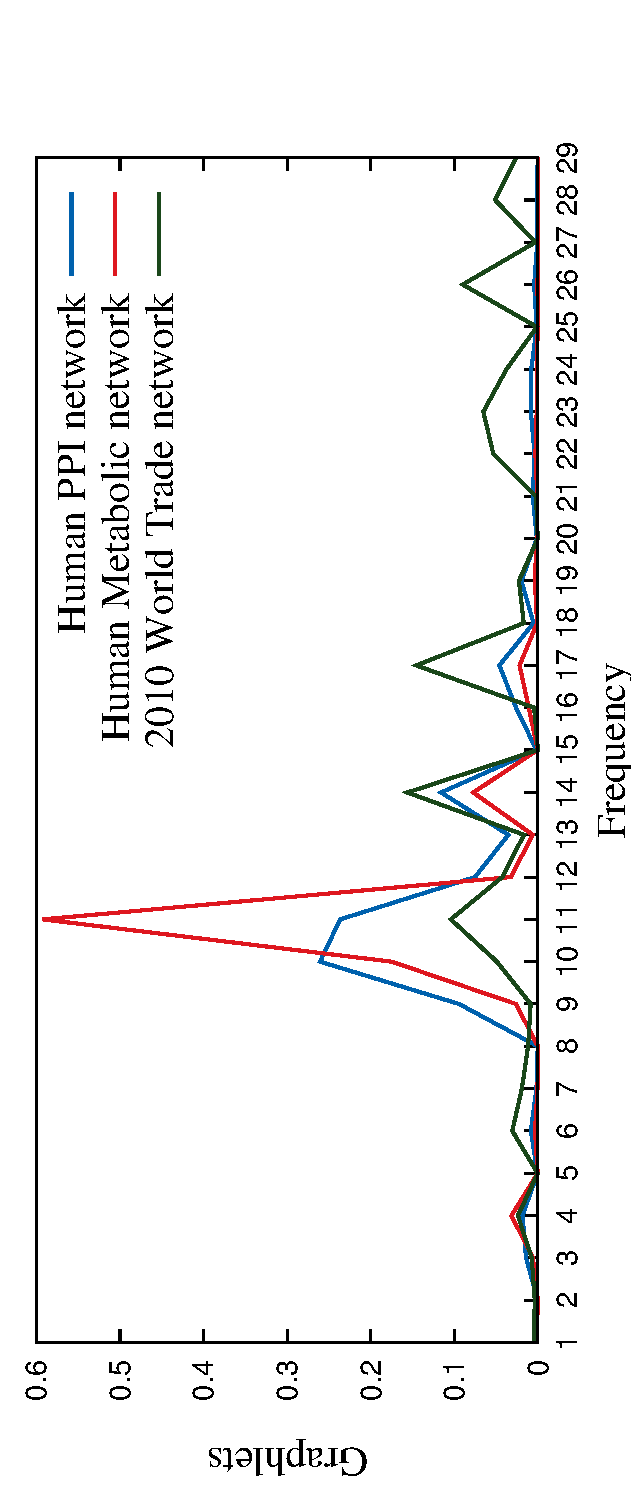
\includegraphics[scale=0.7, angle=-90]{../code/final_results/all_nets_average2.pdf}
  \caption[Average GCV signatures for PPI, Metabolic and World Trade network]{Comparison of the average GCV signatures for three different
  real networks: a PPI network, a Metabolic network and 
  a 2010 World Trade network (WTN). There is a considerable discrepancy in the values of graphlets \{9,10,11\} across the network types. Moreover, the WTN is the only network in which graphlets \{22,23,24,26,28,29\} are represented.}
  \label{fig:avg_gdv_real}
\end{figure}

We observe in figure \ref{fig:avg_gdv_real} that there are slight differences between the normalised GCV of the three networks analysed. More precisely,
Graphlets \{9,10,11\} seem to discriminate well between them, with the Metabolic network having the highest number of $ G_{11}$ graphlets and the WTN having the least. All these graphlets are sparse 5-node graphlets that have 4 edges each. The reason why the Metabolic network has a lot of graphlets $G_{11}$ (a claw of 5 nodes) is because it is made of long metabolic paths that intersect with each other. This is best represented by graphlet $G_{11}$ which is made of a central node and several satellite nodes. Moreover, the WTN also seems to have relatively more graphlets \{22,26,28,29,22,23,24\} compared to the other networks. The reason for this is because the WTN is a dense network and all those graphlets are relatively dense compared to graphlets \{9,10,11, \dots \} that have few connecting edges.

\subsection{Random Networks}
\label{sec:initial_experiments_rnd_nets}

After we performed comparisons of the average GCV of real networks, our
next step is to experiment with the following random network models:
\begin{enumerate}
  \item Erd\H{o}s-R\'{e}nyi \cite{erdHos1959random} (ER)
  \item Erd\H{o}s-R\'{e}nyi (with preserved\footnote{The "stubs" method enables the Erd\H{o}s-R\'{e}nyi graph to preserve the degree distribution of the real network.} degree distribution) (ER-DD)
  \item Geometric networks \cite{penrose2003random} (GEO)
  \item Scale-free Barab\'{a}si-Albert -- preferential attachment \cite{barabasi1999emergence} (SF)
  \item Stickiness index-based \cite{prvzulj2006modelling} (STICKY)
\end{enumerate}


The corresponding labels (ER, ER-DD, GEO, SF, STICKY) will be used throughout this section to refer to each of these models. We generate 30 different models for every network (Metabolic, PPI, WTN) and random network generating algorithm (ER, ER-DD, etc ..) resulting in 150 total networks. Afterwards, in order to give a measure of precision to the GCV signature of random networks, we calculate the standard deviation for each of the values of the GCV. 

The results obtained for the Human PPI network are shown in figure \ref{ppi_spreads}. For the Human PPI network, we notice that all the random models apart from ER-DD have very low standard deviations for all the graphlet frequencies. The graphlets where the ER-DD networks exhibit some degree of randomness are \{10, 11\}. On the other hand, the geometric random graphs are the only ones which contain some of the dense 5-node graphlets at the right-end of the spectrum \{23,24,26,28,29\}. Moreover, the ER random graphs only contain graphlet $G_1$, which is a $P3$. The reason for this is because ER is a rudimentary random graph model that is unable to capture the underlying complexity of the original graph. The random networks that seem to best approximate the original networks are the Scale-free\footnote{Barab\'{a}si-Albert Preferential Attachment} and the Stickiness-based. These results are confirmed by the \emph{Relative Cluster Frequency Agreement} in section \ref{rcfd_res}.


\begin{figure}[H]
  \centering
  \textbf{Average GCV for random models of the Human PPI network}
  \begin{subfigure}[b]{1.0\textwidth}
    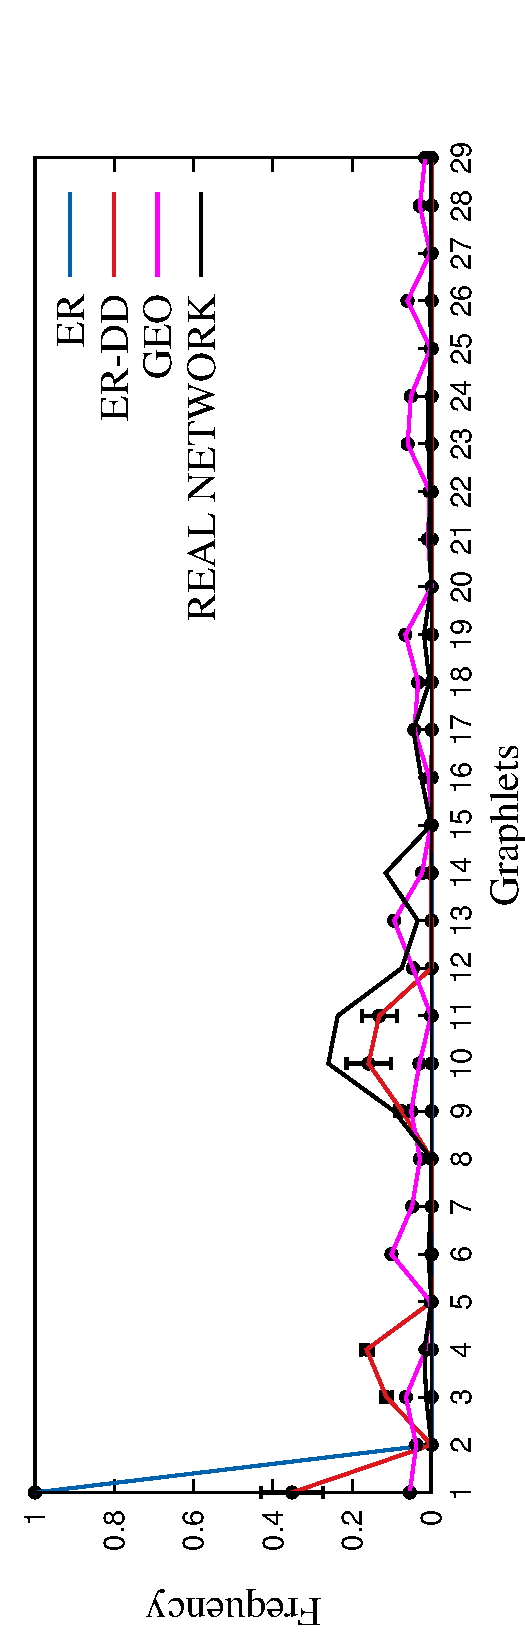
\includegraphics[angle=-90,scale=0.6]{../code/final_results/human_ppi/avg_egdvs_rnd_spreads_figures/spreads_012_rnd2.pdf} 
  \end{subfigure}
  \begin{subfigure}[b]{1.0\textwidth}
    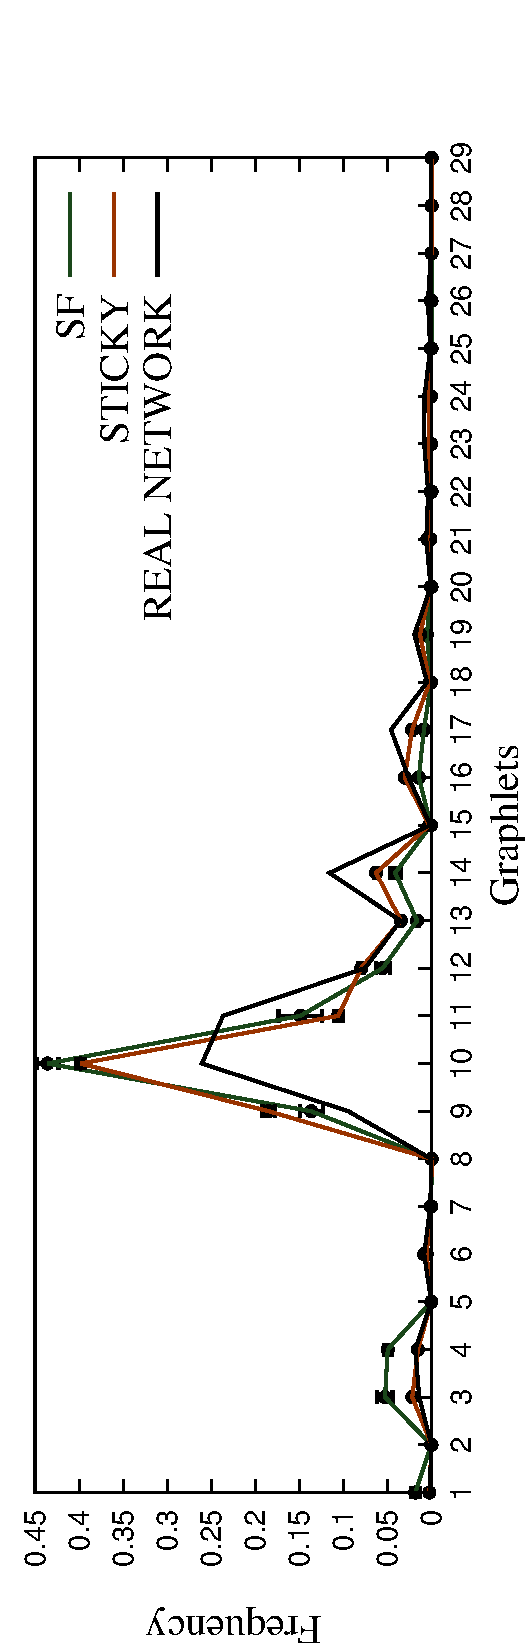
\includegraphics[angle=-90,scale=0.6]{../code/final_results/human_ppi/avg_egdvs_rnd_spreads_figures/spreads_34_rnd2.pdf} 
  \end{subfigure}
\caption[Average GCV for the Human PPI network and ER, ER-DD, GEO, SF and STICKY random models]{Average GCV for the Human PPI network, including the standard deviations displayed as vertical error bars. The random models analysed are: Erd\H{o}s-R\'{e}nyi (ER), Erd\H{o}s-R\'{e}nyi with preserved degree distribution (ER-DD), Geometric (GEO), Scale-free Barab\'{a}si-Albert -- Preferential Attachment (SF) and 
Stickiness-based (STICKY). The length of one vertical bar is equal to one standard deviation $\sigma$. We assume that the samples are normally distributed with mean $\mu$ and variance $\sigma^2$}
\label{ppi_spreads}
\end{figure}

Figure \ref{meta_spreads} shows the average GCVs for the Metabolic networks and the corresponding random networks. We notice that the metabolic networks have a slightly different signature compared to the PPI networks. First of all, they have more graphlets $G_{11}$ but less graphlets $G_{10}$. Secondly, for this class of networks the ER-DD random network seems to be a better approximation according to the GCV signatures, especially for graphlet types \{10,11,12\}. The fact that ER-DD is the best approximation for the Metabolic network is again confirmed in section \ref{rcfd_res}.

\begin{figure}[H]
  \centering
  \textbf{Average GCV for random models of the Human Metabolic network}
  \begin{subfigure}[b]{1.0\textwidth}
    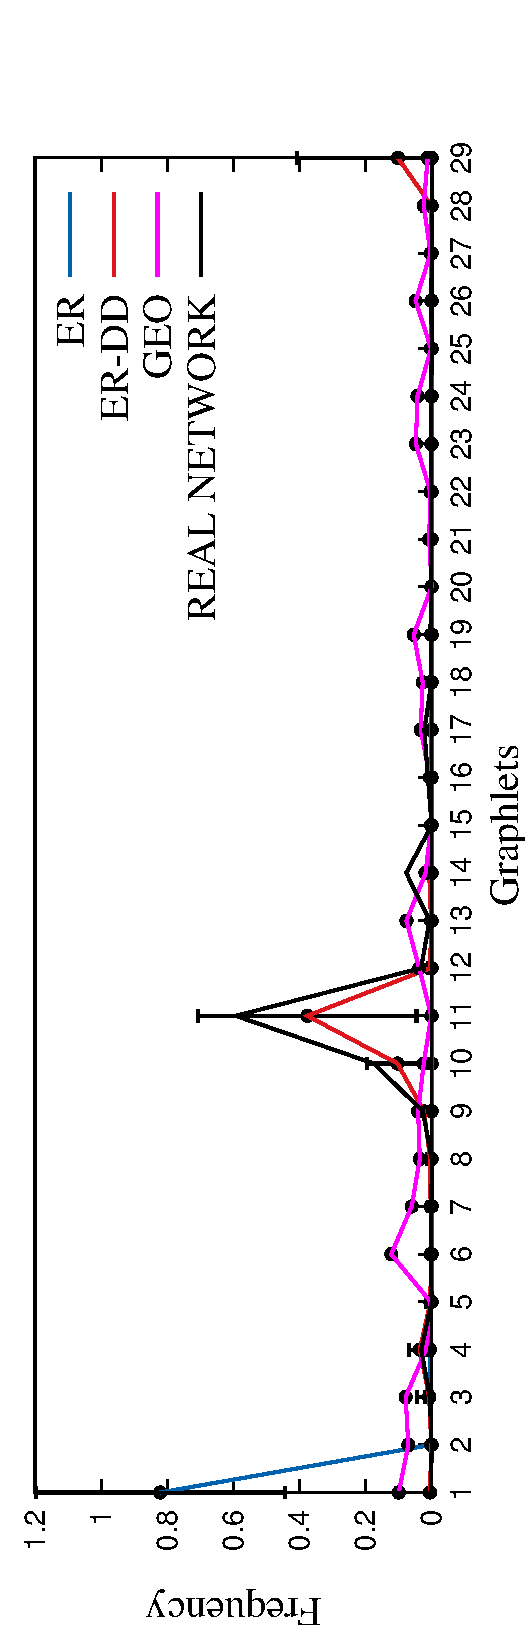
\includegraphics[angle=-90,scale=0.6]{../code/final_results/hsa_metabolic_network/avg_egdvs_rnd_spreads_figures/spreads_012_rnd2.pdf} 
  \end{subfigure}
  \begin{subfigure}[b]{1.0\textwidth}
    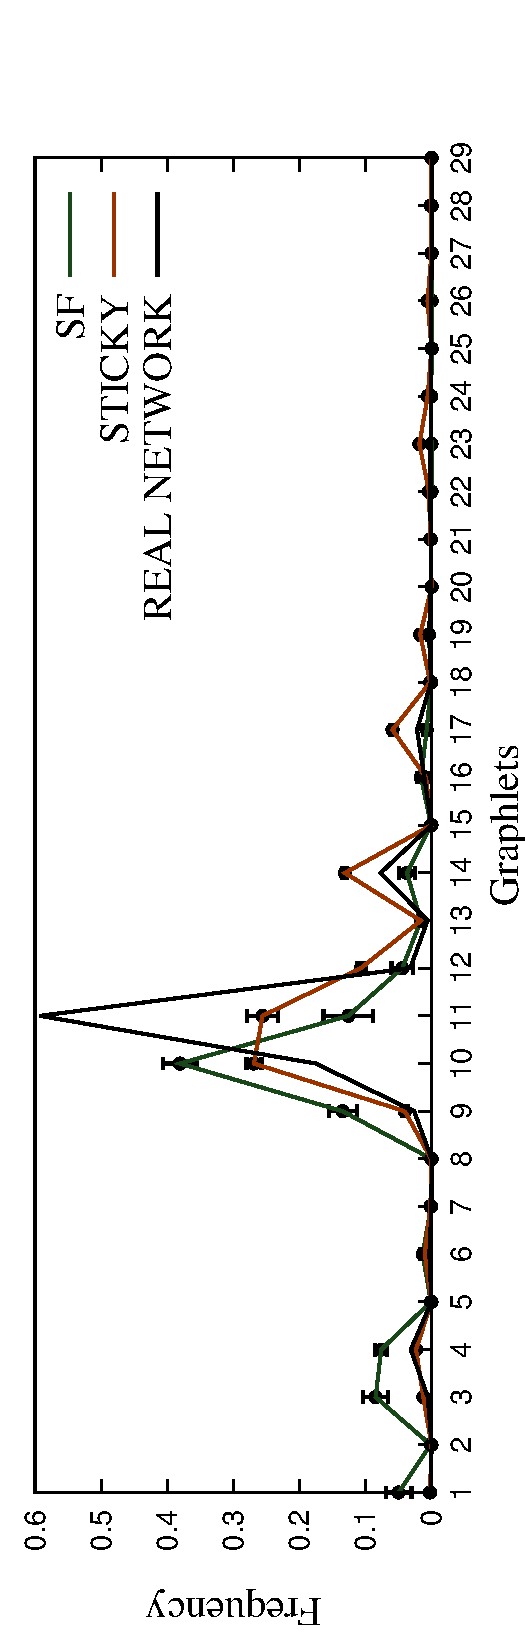
\includegraphics[angle=-90,scale=0.6]{../code/final_results/hsa_metabolic_network/avg_egdvs_rnd_spreads_figures/spreads_34_rnd2.pdf} 
  \end{subfigure}
  \caption[Average GCV for the Human Metabolic network and ER, ER-DD, GEO, SF and STICKY random models]{Average GCV for the Human Metabolic network, including the standard deviations displayed as vertical error bars. The random models analysed are: Erd\H{o}s-R\'{e}nyi (ER), Erd\H{o}s-R\'{e}nyi with preserved degree distribution (ER-DD), Geometric (GEO), Scale-free Barab\'{a}si-Albert -- Preferential Attachment (SF) and Stickiness-based (STICKY). The length of one vertical bar is equal to one standard deviation $\sigma$. We assume that the samples are normally distributed with mean $\mu$ and variance $\sigma^2$}
  \label{meta_spreads}
\end{figure}

Figure \ref{trade_spreads} shows the average GCVs for the WTNs and the corresponding random graphs. Surprisingly, for this type of networks we see a greater variety in the frequencies of graphlets, with graphlets in the 15--29 range now being much more represented than in the biological networks. The simple Erd\H{o}s-R\'{e}nyi model has a large variance for the frequency of graphlets \{3,9,10\}. On the other hand, the Erd\H{o}s-R\'{e}nyi graphs with preserved degree distribution offer a good GCV signature approximation, especially for graphlets in the range \{9-18\}, which are the 5-node graphlets at the sparse end of the spectrum. The Stickiness-based random graphs also offer a good approximation, a result that is confirmed by the \emph{Relative Cluster Frequency Agreement} in section \ref{rcfd_res}.

\begin{figure}[H]
  \centering
  \textbf{Average GCV for random models of the 2010 World Trade Networks}
  \begin{subfigure}[b]{1.0\textwidth}
    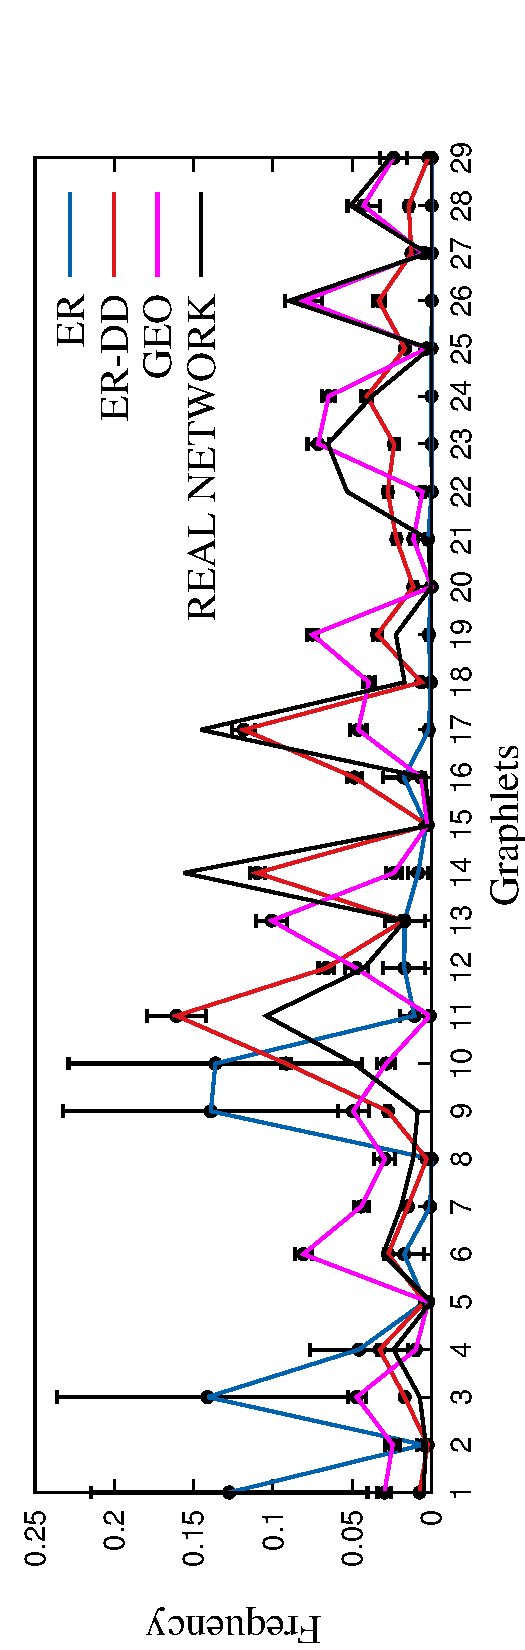
\includegraphics[angle=-90,scale=0.6]{../code/final_results/trade_2010_thresholded/avg_egdvs_rnd_spreads_figures/spreads_012_rnd2.pdf} 
  \end{subfigure}
  \begin{subfigure}[b]{1.0\textwidth}
    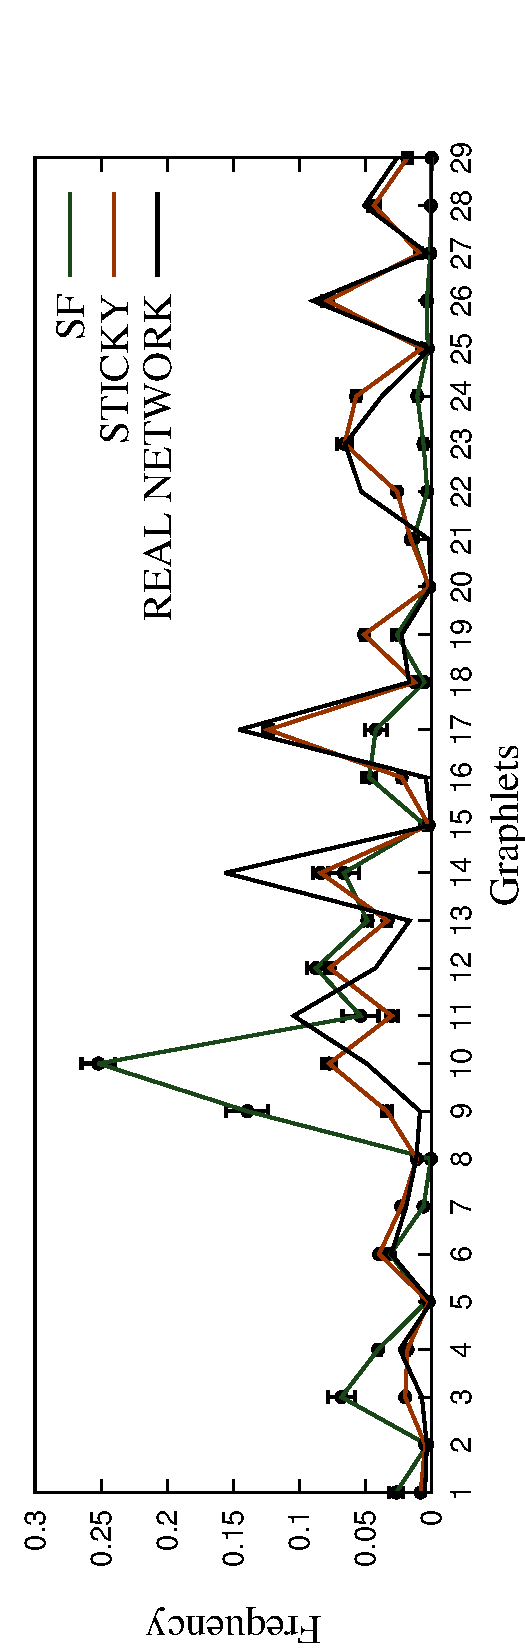
\includegraphics[angle=-90,scale=0.6]{../code/final_results/trade_2010_thresholded/avg_egdvs_rnd_spreads_figures/spreads_34_rnd2.pdf} 
  \end{subfigure}
  \caption[Average GCV for the World Trade network and ER, ER-DD, GEO, SF and STICKY random models]{Average GCV for the 2010 WTN, including the standard deviations displayed as vertical error bars. The random models analysed are: Erd\H{o}s-R\'{e}nyi (ER), Erd\H{o}s-R\'{e}nyi with preserved degree distribution (ER-DD), Geometric (GEO), Scale-free Barab\'{a}si-Albert -- Preferential Attachment (SF) and 
Stickiness-based (STICKY). The length of one vertical bar is equal to one standard deviation $\sigma$. We assume that the samples are normally distributed with mean $\mu$ and variance $\sigma^2$}
  \label{trade_spreads}
\end{figure}


\subsection{Relative Cluster Frequency Distance Results}
\label{rcfd_res}

The \emph{Relative Cluster Frequency Distance} (RCFD) between two GCV vectors is a measure of how different they are with each other. It it is defined as the Euclidean norm of the difference between the two GCV vectors. A low RCFD value means that the signatures are similar to each other, while a high value means that the signatures are different. See section \ref{rcfd} for the exact definition of RCFD. When applied to the average GCV signature of two networks, RCFD can tell us how similar or different the two networks are. The question we are trying to answer here is: according to the average GCV signature, which random graph is best for modelling the real underlying network? The three tables from figure \ref{gcv_agr} show the RCFD distances between the real network and random models\footnote{the real network has been used to generate these random models}, applied to our three main classes of networks: PPI, Metabolic and World Trade. 

For the Human PPI network (table (\subref{tab:rcfd_ppi}) from fig \ref{gcv_agr}), the random networks that best approximate the real network are the Stickiness-based (STICKY) random networks, having the smallest RCFD of 0.492, while the Scale-free Barab\'{a}si-Albert (SF) graphs also offer a good approximation of the original network, having a RCFD of 0.607. The other random models perform much worse in this respect because they cannot capture all the underlying complexity in the dataset. Moreover, we also notice that the difference between the SF and STICKY GCV signatures is really small (0.329), meaning that the generated networks are topologically similar to each other.

For the Human Metabolic network (table (\subref{tab:rcfd_meta}) from fig \ref{gcv_agr}), the results are slightly different. The best-performing random networks are the ER-DD (RCFD to the real network is 0.557), built using the "stubs" method (see section \ref{er-dd}). The second-best random network is the STICKY model which has an RCFD between itself and the Real network of 0.697. When analysing the 2010 WTN between countries(table (\subref{tab:rcfd_trade}) from fig \ref{gcv_agr}), the random network with the best approximation to the real network is again the Stickiness-based network, followed closely by Erd\H{o}s-R\'{e}nyi with preserved degree distribution.

We therefore conclude that the STICKY random model is best at modelling PPI and WTN networks, while ER-DD is best at modelling Metabolic networks.

\rowcolors{1}{blue1}{blue2}

%     Relative Cluster Frequency Distance for the Human PPI network\\
\newcommand{\humanppiagr}{% Just for this example
      \begin{tabular}{ c | c  c  c  c  c | c }
      Model & ER & ER DD & GEO & SF & STICKY & REAL\\
      \hline
      ER     & 0.000 & 1.296 & 1.889 & 1.963 & 1.995 & 1.995 \\
      ER DD  & 1.296 & 0.000 & 1.554 & 1.018 & 1.233 & 1.191 \\
      GEO    & 1.889 & 1.554 & 0.000 & 1.413 & 1.406 & 1.311 \\
      SF     & 1.963 & 1.018 & 1.413 & 0.000 & 0.329 & 0.607 \\
      STICKY & 1.995 & 1.233 & 1.406 & 0.329 & 0.000 & \textbf{0.492} \\
      \hline
      REAL   & 1.995 & 1.191 & 1.311 & 0.607 & \textbf{0.492} & 0.000\\
      \end{tabular}
}

%     Relative Cluster Frequency Distance for the Human Metabolic network\\
\newcommand{\hsametaagr}{% Just for this example
    \begin{tabular}{ c | c  c  c  c  c | c }
    Model & ER & ER DD & GEO & SF & STICKY & REAL\\
    \hline
    ER     & 0.000 & 1.499 & 1.610 & 1.709 & 1.804 & 1.807\\
    ER DD  & 1.499 & 0.000 & 1.430 & 1.040 & 0.799 & \textbf{0.557}\\ 
    GEO    & 1.610 & 1.430 & 0.000 & 1.356 & 1.438 & 1.648\\
    SF     & 1.709 & 1.040 & 1.356 & 0.000 & 0.784 & 1.054\\
    STICKY & 1.804 & 0.799 & 1.438 & 0.784 & 0.000 & 0.697\\
    \hline
    REAL   & 1.807 & \textbf{0.557} & 1.648 & 1.054 & 0.697 & 0.000\\
    \end{tabular}
}

%     Relative Cluster Frequency Distance for the Trade 2010 thresholded network\\
\newcommand{\tradeagr}{% Just for this example
    \begin{tabular}{ c | c  c  c  c  c | c }
    Model & ER & ER DD & GEO & SF & STICKY & REAL\\
    \hline
    ER     & 0.000 & 1.134 & 1.198 & 0.663 & 1.172 & 1.336 \\
    ER DD  & 1.134 & 0.000 & 1.065 & 0.819 & 0.490 & 0.572 \\
    GEO    & 1.198 & 1.065 & 0.000 & 1.099 & 0.609 & 0.873 \\
    SF     & 0.663 & 0.819 & 1.099 & 0.000 & 0.896 & 1.161 \\
    STICKY & 1.172 & 0.490 & 0.609 & 0.896 & 0.000 & \textbf{0.465} \\
    \hline
    REAL   & 1.336 & 0.572 & 0.873 & 1.161 & \textbf{0.465} & 0.000\\
    \end{tabular}

}


\begin{figure}[H]%
  \centering
  \vspace{1em}
  \begin{subfigure}{1.0\textwidth}
    \centering
    \humanppiagr   
    \caption{RCFD distances for the Human PPI network}
    \vspace{1.5em}
    \label{tab:rcfd_ppi}
  \end{subfigure}
%   \qquad
%   \hspace{5em}
  \begin{subfigure}{1.0\textwidth}
    \centering
    \hsametaagr   
    \caption{RCFD distances for the Human Metabolic network}
    \vspace{1.5em}
    \label{tab:rcfd_meta}
  \end{subfigure}
%   \vspace{1em}
  \begin{subfigure}{1.0\textwidth}
    \centering
    \tradeagr 
    \caption{RCFD distances for the 2010 World Trade network}
    \label{tab:rcfd_trade}
  \end{subfigure}
%   \subfloat[][]{}
%   \qquad
%   \subfloat[][]{}
  \caption[RCFD distances for the Human PPI, Human Metabolic and WTN networks.]{The RCFD distances for (\subref{tab:rcfd_ppi}) Human PPI network (\subref{tab:rcfd_meta}) Human Metabolic network (\subref{tab:rcfd_trade}) 2010 WTN and five model networks: Erd\H{o}s-R\'{e}nyi (ER), Erd\H{o}s-R\'{e}nyi with preserved degree distribution (ER DD), Geometric (GEO), Scale-Free - Barab\'{a}si-Albert Preferential Attachment (SF) and Stickiness-based (STICKY). For each network class, we have calculated not only the distance between every pair of random network models, but also the distance between every random network model and the real network which was used to generate the random models.}
  \label{gcv_agr}%
\end{figure}

% \begin{figure}[H]%
%   \centering
%   \subfloat[][]{\humanppiagr}
%   \qquad
%   \subfloat[][]{\hsametaagr}
%   \qquad
%   \subfloat[][]{\tradeagr}
%   \caption[RCFD distances for the Human PPI, Human Metabolic and WTN networks.]{The RCFD distances for (a) Human PPI network (b) Human Metabolic network (c) 2010 WTN and five model networks: Erd\H{o}s-R\'{e}nyi (ER), Erd\H{o}s-R\'{e}nyi with preserved degree distribution (ER DD), Geometric (GEO), Scale-Free - Barab\'{a}si-Albert Preferential Attachment (SF) and Stickiness-based (STICKY). For each network class, we have calculated not only the distance between every pair of random network models, but also between every random network model and the real network which was used to generate the random models}
%   \label{gcv_agr}%
% \end{figure}



\section{World Trade networks}
\label{trade_res_heatmaps}

After running initial experiments that study the average GCV of a network, we performed experiments that were specific to each of the network classes. In this section, we present the main results obtained for the World Trade Networks (WTNs). A brief summary of these networks is given in section \ref{sec:trade_bck}. 

\begin{figure}[H]
  \begin{center}
  \hbox{\hspace{-1cm}
  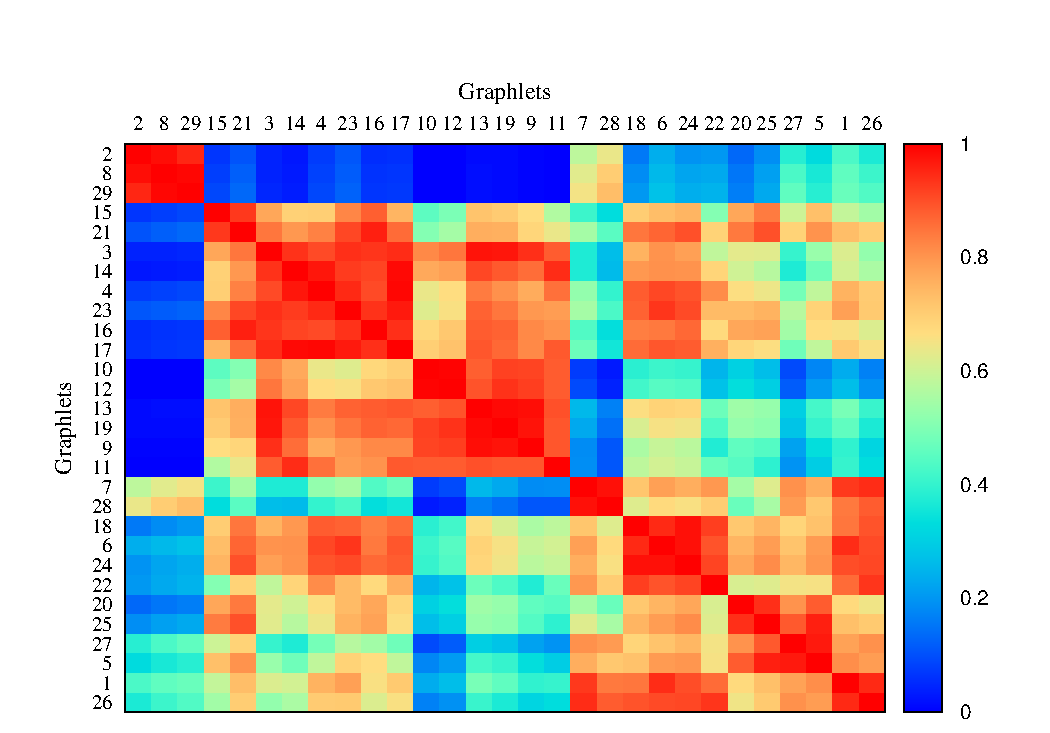
\includegraphics[scale=1.0]{../code/final_results/trade_2010_thresholded/heatmap_pearsons_hclust_trade_2010_thresholded-poly-32.pdf}} 
  \caption[Pearson's GCV correlation matrix for the 2010 WTN]{Pearson's GCV correlation matrix for the 2010 WTN. It has been normalised with feature scaling and a $3^{rd}$ degree polynomial, and then hierarchically clustered with complete linkage.}
  \label{fig:trade_heatmap}
  \end{center}
\end{figure}


Figure \ref{fig:trade_heatmap} shows the \emph{Pearson's GCV Correlation matrix} for the 2010 WTN. This correlation matrix was normalised with feature scaling and a $3^{rd}$ degree polynomial function. For details on how this has been calculated see the methodology section \ref{sec:metho_pears}. Other polynomial functions have been tested, but the $3^{rd}$ degree polynomial was the most effective in emphasising the clusters of graphlets that are formed on the diagonal. These clusters of graphlets are as follows:
\begin{itemize}
 \item Cliques cluster made of graphlets \{2,8,29\}.
 \item A cluster that is made of graphlets \{15,21,3,14,4,23,16,17,10,12,13,19,9,11\} which can be split into 2 further sub-clusters: 
    \begin{itemize}
     \item $P_4$ cluster made of graphlets \{15,21,3,14,4,23,16,17\}. These are all 
     graphlets that contain a $P_4$ (path of 4 nodes, graphlet $G_3$). 
     \item Claw\footnote{A claw $C_n$ is a graphlet that has a central node and $n-1$ satellite nodes connected to it. See section \ref{graph_terminology} for a full definition.} cluster made of \{10,12,13,19,9,11\}. These graphlets all contain a $C_3$ ( claw on 3 nodes, graphlet $G_4$)
    \end{itemize}
 \item A cluster that is made of graphlets \{20,25,27,5\}. These graphlets all contain an $S_4$ (cycle of 4 nodes).   
 \item Another set of graphlets that correlate is \{18,6,24,22,1,26\}. The reason why graphlets \{1,26\} have been added is because they also correlate with the other cluster, even if they are not right next to them in the heat map. These all contain at least one $P_3$ (path of 3 nodes).
\end{itemize}

Now that we know which graphlets cluster together, we will use these results in the subsequent CCA analysis in section \ref{sec:cca_orig}.

\subsection{Correlation matrix change during 1962--2010}
\label{trade_change_orig}

%gcv offset: -2   Spearman's rank coefficient: corr: -0.493973099551    p_value: 0.000485081849961
The results from the previous section were concerned with the correlation matrix of the 2010 WTN. However, we are also interested to see how graphlets correlate in WTNs from other years. We therefore compute the Pearson's GCV correlation matrix for all the yearly WTNs in the period 1962--2010. Using the 49 different correlation matrices, we then compute the \emph{change in the correlation matrix} during the respective time frame. In order to calculate the change in correlation matrix between year $Y$ and $Y+1$, we simply subtract in a pairwise manner the two matrices and then return the sum of squares of all the elements in the matrix. For the exact formula used see equation \ref{pears_matrix_diff} from section \ref{pearsons_background}. 

We then tried to find out if there is any correlation between the network topology and Crude Oil price. If one of these attributes changes, it might be possible that the other reacts. However, this might happen with a certain number of years delay. In order to account for this, we shift the vector of GCV correlation change by [-2,-1,0,1,2] years. For each of these 5 cases, we calculate the \emph{Spearman's rank correlation coefficient} and the respective p-value for the following vectors:
\begin{itemize}
 \item one 48-element vector containing the \emph{change in Pearson's GCV correlation matrix}
 \item one 48-element vector containing the \emph{change in the price of Crude Oil}
\end{itemize}


The best correlation is obtained when the vector of GCV correlation is shifted by -2 years. This scenario is plotted in figure \ref{change_over_time_orig}. Surprisingly, the oil change in inversely correlated with the change in network topology: the Spearman's rank correlation coefficient is -0.49, having a p-value of 0.0004. Since the p-value is smaller than 0.05, the result is statistically significant. The explanation for this is as follows: high oil prices generally have a large negative impact on the global economic growth. Slower growth leads to diminished investment-related activity in the countries affected, which in turn deters the creation of new trading partners. This implies that the network structure remains mostly unchanged, a fact that results in a low GCV correlation change. Moreover, because the best correlation is obtained when the change in GCV is shifted by -2 years, this might suggest that changes in network structure cause the Crude Oil price to change. However, we did not have time to 
perform more supporting experiments in order to validate the causality aspect of this claim.

Furthermore, there are several major economic events for which we do not have a big change in the topology of our network, such as the 2007 sub-prime mortgage crisis or the 1997 Asian financial crisis. This implies that the unnormalised Pearson's GCV correlation matrix is not affected by these major events. Similar results that use a normalised version of the GCV are better correlated with global economic and social events (see section \ref{rev_trade_change}).

\begin{figure}[H]
  \centering
  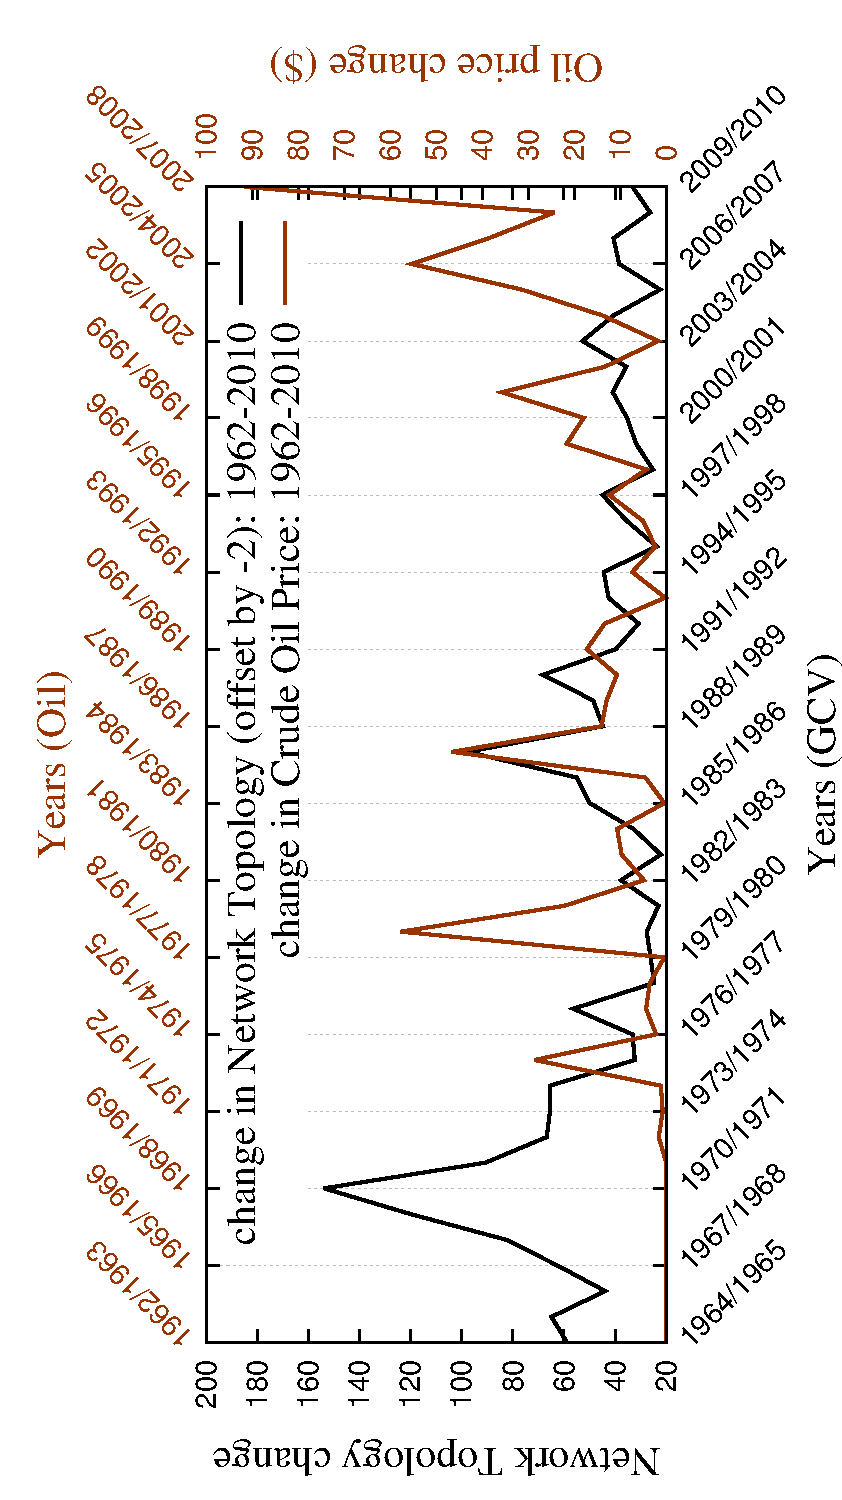
\includegraphics[angle=-90,scale=0.6]{../code/final_results/all_trade_thresh/change_over_time2}
% \mbox{\epsfbox{../code/final_results/all_trade_thresh/change_over_time}}
\caption[Evolution of WTN structure during 1962--2010 - unnormalised GCV]{Evolution of WTN structure during 1962--2010 using the unnormalised GCV. Plotted in black is the change in GCV correlation that has been offset by -2 years, while the change in Crude Oil Price is plotted in brown. Spearman's rank coefficient between oil price change and change in network topology is -0.49 with a p-value of 0.0004. This suggests that when the change in GCV correlation between countries changes, then the oil price stays the same. The top and left axis tics correspond to the Oil curve, while the bottom and the left axis tics correspond to the network topology curve.}
\label{change_over_time_orig}
\end{figure}

% Omer - 1993 is computed as (Price_{1993} - Price_{1992}). The graph however shows 1993/1992 or smth similar

\subsection{CCA - 1980--2010 World Trade networks}
\label{sec:cca_orig}
After correlating graphlets from the GCV vector with each other in order to see which one of them have a similar behaviour, the next step is to correlate the GCV vectors with the economic indicators of a country. This can be done using \emph{Canonical Correlation Analysis} (CCA) which is described in section \ref{cca_background}. The two variates we correlated are:
\begin{enumerate}
 \item the X variate containing economic indicators (GDP per Capita, Level of Employment). See section \ref{sec:trade_bck} for details about all the economic indicators used.
 \item the Y variate containing the unnormalised GCV vectors for each country.
\end{enumerate}

The CCA analysis uses data for 119 countries over a period of 30 years (1980-2010). Each country-year pair represents one sample for which we have both economic indicators (X variate) and the GCV (Y variate).



\newcommand{\ccaIndicatorsTradeUnnorm}{
  \begin{tabular}{r}
  \cellcolor{black}\textcolor{ccacol1}{POP}\\
  \cellcolor{black}\textcolor{ccacol1}{LE}\\
  \cellcolor{black}\textcolor{ccacol1}{KI x RGDPL x POP}\\
  \cellcolor{black}\textcolor{ccacol1}{RGDPCH x POP}\\
  \cellcolor{black}\textcolor{ccacol1}{RGDPL x POP}\\
  \cellcolor{black}\textcolor{ccacol1}{RGDPL2 x POP}\\
  \cellcolor{black}\textcolor{ccacol1}{KC x RGDPL x POP}\\
  \cellcolor{black}\textcolor{ccacol1}{KG x RGDPL x POP}\\
  \cellcolor{black}\textcolor{ccacol2}{KC x RGDPL}\\
  \cellcolor{black}\textcolor{ccacol3}{RGDPCH}\\
  \cellcolor{black}\textcolor{ccacol3}{RGDPL}\\
  \cellcolor{black}\textcolor{ccacol3}{RGDPL2}\\
  \cellcolor{black}\textcolor{ccacol3}{KG x RGDPL}\\
  \cellcolor{black}\textcolor{ccacol4}{KI x RGDPL}\\
  \cellcolor{black}\textcolor{ccacol4}{XRAT}\\
  \cellcolor{black}\textcolor{ccacol4}{KC}\\
  \cellcolor{black}\textcolor{ccacol5}{KI}\\
  \cellcolor{black}\textcolor{ccacol5}{BCA per RGDPL}\\
  \cellcolor{black}\textcolor{ccacol5}{KG}\\
  \cellcolor{black}\textcolor{ccacol6}{BCA}\\
  \cellcolor{black}\textcolor{ccacol6}{OPENK}
  \end{tabular}

}


\begin{figure}[H]
  \centering
    \begin{tikzpicture}[scale=\ccafigscale,show background rectangle, 
  background rectangle/.style={fill=black},
  color=white,help lines/.style={color=lightgray,line width=0.2pt},post/.style={->,shorten >=1pt,>=stealth',thick}]

    \node[upper left,inner sep=0,scale=\ccafigscale] (indicators) at (-2.0,0) {\ccaIndicatorsTradeUnnorm};	
    \shade[top color=green,bottom color=yellow] (4,0) rectangle (4.5,5);
    \shade[top color=yellow,bottom color=red] (4,-5) rectangle (4.5,0);
    \node[upper left,inner sep=0] (dummy) at (13.0,4) {}; % for extending the black bounding box
    \node[upper left,inner sep=0,scale=\ccafigscale * 1.3] (corr_text) at (4.25,-6.0) {Correlation};
    \node[upper left,inner sep=0,red] (corr_text) at (4.25,-5.5) {-1};
    \node[upper left,inner sep=0, green] (corr_text) at (4.25,5.5) {1};
    \node[upper left,inner sep=0] (corr_text) at (4.75,0) {0};
    
    \node[upper left,inner sep=0,scale=\ccafigscale] (g1) at (7.5,5) {\gonecca{ccacol1}};
    \node[upper left,inner sep=0,scale=\ccafigscale] (g2) at (10.5,3.5) {\gtwocca{ccacol1}};
    \node[upper left,inner sep=0,scale=\ccafigscale] (g6) at (7.5,2) {\gsixcca{ccacol1}};
    \node[upper left,inner sep=0,scale=\ccafigscale] (g16) at (10.5,-2.5) {\gsixteencca{ccacol3}};
    \node[upper left,inner sep=0,scale=\ccafigscale] (g15) at (7.5,-4) {\gfifteencca{ccacol3}};
    \node[upper left,inner sep=0,scale=\ccafigscale] (g20) at (10.5,-5.5) {\gtwentycca{ccacol3}};
    
    \draw[line,color=white] (6,0) -- (13.00,0);
    \node[upper left,inner sep=0,scale=\ccafigscale * 1.3] (strong_corr) at (10,0.5) {Highest correlations};    
    \node[upper left,inner sep=0,scale=\ccafigscale * 1.3] (strong_corr) at (10,-0.5) {Lowest correlations};    
    
    \draw[line,color=ccacol1] (0.00,4.80) -| (1.64,3.83) -- (4.00,3.83);
    \draw[line,color=ccacol1] (0.00,4.33) -| (1.15,3.79) -- (4.00,3.79);
    \draw[line,color=ccacol1] (0.00,3.85) -| (0.8,3.63) -- (4.00,3.63);
    \draw[line,color=ccacol1] (0.00,3.38) -| (0.8,3.59) -- (4.00,3.59);
    \draw[line,color=ccacol1] (0.00,2.90) -| (1.2,3.59) -- (4.00,3.59);
    \draw[line,color=ccacol1] (0.00,2.42) -| (1.3,3.58) -- (4.00,3.58);
    \draw[line,color=ccacol1] (0.00,1.95) -| (1.4,3.50) -- (4.00,3.50);
    \draw[line,color=ccacol1] (0.00,1.48) -| (1.5,3.47) -- (4.00,3.47);
    \draw[line,color=ccacol2] (0.00,1.00) -| (1.6,2.10) -- (4.00,2.10);
    \draw[line,color=ccacol3] (0.00,0.53) -| (1.7,1.33) -- (4.00,1.33);
    \draw[line,color=ccacol3] (0.00,0.05) -| (1.9,1.33) -- (4.00,1.33);
    \draw[line,color=ccacol3] (0.00,-0.42) -| (2.1,1.33) -- (4.00,1.33);
    \draw[line,color=ccacol3] (0.00,-0.90) -| (2.3,1.09) -- (4.00,1.09);
    \draw[line,color=ccacol4] (0.00,-1.38) -| (2.5,0.89) -- (4.00,0.89);
    \draw[line,color=ccacol4] (0.00,-1.85) -| (2.7,0.60) -- (4.00,0.60);
    \draw[line,color=ccacol4] (0.00,-2.33) -| (2.8,0.49) -- (4.00,0.49);
    \draw[line,color=ccacol5] (0.00,-2.80) -| (3,-0.30) -- (4.00,-0.30);
    \draw[line,color=ccacol5] (0.00,-3.27) -| (3.2,-0.74) -- (4.00,-0.74);
    \draw[line,color=ccacol5] (0.00,-3.75) -| (3.4,-0.87) -- (4.00,-0.87);
    \draw[line,color=ccacol6] (0.00,-4.23) -| (3.6,-1.00) -- (4.00,-1.00);
    \draw[line,color=ccacol6] (0.00,-4.70) -| (3.8,-1.24) -- (4.00,-1.24);



    
    
    \draw[line,color=ccacol1] (g1) -| (6.1,4.2) -- (4.5,4.2);
    \draw[line,color=ccacol1] (g2) -| (5.9,4.05) -- (4.5,4.05);
    \draw[line,color=ccacol1] (g6) -| (5.7,4.0) -- (4.5,4.0);

    \draw[line,color=ccacol3] (g16) -| (5.5,2.8) -- (4.5,2.8);
    \draw[line,color=ccacol3] (g15) -| (5.3,2.5) -- (4.5,2.5);
    \draw[line,color=ccacol3] (g20) -| (5.1,2.2) -- (4.5,2.2);
    
    \end{tikzpicture}
    \caption[CCA - World Trade networks - unnormalised GCV - Picture version]{Canonical Correlation Analysis between economic indicators and the GCV signature. Only the graphlets that have the highest respectively lowest cross-loadings are shown in the picture. However, all the graphlets have positive cross-loadings, with the lowest cross-loading having a value of 0.44. Openness (OPENK), Balance Current Account (BCA) and a few other indicators correlate negatively with all the graphlets, because their cross-loadings have different signs. On the other hand, the rest of the indicators such as Population (POP), Level of Employment (LE) and GDP per capita (RGPDL, RGDPCH) correlate positively with all the graphlets, since their cross-loadings have the same sign. The overall correlation is 0.89 with a p-value smaller than 0.0001. This result suggests that big and wealthy countries have a large network of trading partners that is rich in graphlets.}
    \label{fig:all_trade_cca_unnorm_black}	
\end{figure}


CCA results are presented in figure \ref{fig:all_trade_cca_unnorm_black}. A supplementary table with the list of all the cross-loadings can be found in figure \ref{all_trade_thresh_cca_orig} in the appendix. This result shows that all the graphlets correlate positively\footnote{An element from the $X$ variate correlates positively with another element from the $Y$ variate if and only if their cross-loadings have the same sign} with some indicators such as Population, Level of Employment or GDP per capita and negatively with Trade Openness and Balance of Current Account. This means that big and rich countries that have a high population and GDP per capita have a neighbourhood rich in graphlets, while small and poor countries with account deficits have a neighbourhood sparse in graphlets. The population of the country seems to be quite an important factor for determining whether it will have a rich neighbourhood because of the following two reasons:
\begin{itemize}
 \item In the $X$ variate, population has the weight with the highest magnitude: 0.766
 \item Most of the other economic indicators that have a high weight are obtained by multiplying population with other indicators. This is also the case in a similar CCA Analysis of Yavero\u{g}lu et al. using graphlet orbits \cite{yaverouglu2014revealing}.
\end{itemize}

\subsection{Economic Integration}
\label{sec:cca_integration}

We now try to find out if the level of \emph{Economic Integration} of a country is positively correlated with dense graphlets and negatively correlated with sparse graphlets. This is something to be expected, because when a country is part of a strong trading bloc, it's neighbours have a higher probability of doing heavy trade with one another. This is because there is incentive for the country to trade more with the partners from the same bloc, that are already trading a lot with each other. This would in turn result in denser graphlets in the neighbourhood of that country. The idea of correlating the GCV with the integration level of a country was entirely mine.

For a given country, there exist several stages of economic integration. One possible classification is the following:
\begin{enumerate}
 \item no economic integration 
 \item Multilateral Free Trade Area (e.g. AFTA, CEFTA, CISFTA)
 \item Customs union (e.g. EAC, EUCU, MERCOSUR)
 \item Common market (e.g. EEA, EFTA) 
 \item Customs and Monetary Union (e.g. CEMAC/franc, UEMOA/franc) 
 \item Economic union (e.g. CSME, EU) 
 \item Economic and monetary union (e.g. CSME + EC dollar, EU + euro)
\end{enumerate}

We found some preliminary data on the Internet which labels each country using the most advanced integration agreement it signed. Using this data, we computed an integration index (1-7) for each country and correlated it with the GCV signature using CCA.


\begin{figure}
  \begin{subfigure}{.65\textwidth}
  \centering
  \begin{tabular}{ c c | c c }
    \multicolumn{2}{c}{Canonical Correlation} &  \multicolumn{2}{c}{0.61882} \\
    \multicolumn{2}{c}{p-value} &  \multicolumn{2}{c}{0.01280} \\
    \hline
    \multicolumn{2}{c}{X variate} & \multicolumn{2}{c}{Y variate}\\
    \hline
  Integration & 0.61882 &  G29 & 0.28704\\
  & &  G8 & 0.28349\\
  & &  G2 & 0.27862\\
  & &  G22 & 0.26820\\
  & &  G28 & 0.26806\\
  & &  G7 & 0.26021\\
  & &  G26 & 0.26011\\
  & &  G18 & 0.24661\\
  & &  G1 & 0.23837\\
  & &  G24 & 0.23133\\
  & &  G6 & 0.22969\\
  & &  G4 & 0.22021\\
  & &  G27 & 0.22013\\
  & &  G17 & 0.21021\\
  & &  G14 & 0.20631\\
  & &  G23 & 0.20420\\
  & &  G5 & 0.20149\\
  & &  G20 & 0.19391\\
  & &  G25 & 0.19122\\
  & &  G21 & 0.19076\\
  & &  G16 & 0.19026\\
  & &  G11 & 0.18330\\
  & &  G3 & 0.17730\\
  & &  G15 & 0.16814\\
  & &  G13 & 0.16764\\
  & &  G19 & 0.16051\\
  & &  G9 & 0.15087\\
  & &  G12 & 0.14886\\
  & &  G10 & 0.14638\\
  \end{tabular}

  \end{subfigure}
  \begin{subfigure}{.25\textwidth}
    \centering 
    \rowcolors{1}{}{}		
    
    \gtwentynine
    \geight
    \gtwo
    \gdots
    \gnine
    \gtwelve
    \gten

  \end{subfigure}
  
\caption[CCA - World Trade Network - Integration index]{CCA results between the Integration index ($X$ variate) and the GCV ($Y$ variate). The Integration index of a country is positively correlated with all the graphlets. However, the strongest correlation is with dense graphlets such as cliques \{29,8,2\} because they have the highest weight, while sparser graphlets \{10,12,9\} have the lowest weight. The overall correlation is 0.61, with a p-value of 0.01, suggesting the correlation is statistically significant.}
\label{trade_2010_thresholded_cca}
\end{figure}


Figure \ref{trade_2010_thresholded_cca} presents these preliminary CCA results. They confirmed our initial expectations, with dense graphlets correlating most with the integration index, while the sparse graphlets correlating least. However, since the source of the data that was used for this experiment could not be verified, we searched for an official index that quantifies political integration for each country around the world. Although we haven't found an index that uses the 6-level scale that we previously mentioned, we found some indices on the \emph{World Trade Organisation} website that measure the number of \emph{Regional Trade Agreements} (RTAs) of a country \cite{rtas2014wto}. These RTAs are defined as trade agreements that are concluded between countries that are geographically close to each other\footnote{However, the countries do not strictly have to be geographically close in order to sign an RTA.}. For a given country, the number of RTAs gives us a measure of economic and political 
integration, since these agreements are mainly signed within trading blocks. The RTAs facilitate trade on a regional basis and can be of several types:
\begin{itemize}
 \item A Free Trade Agreement (FTA)
 \item A Customs Union (CU)
 \item Economic Integration Agreement (EIA)
 \item Partial Scope Agreement\footnote{Covers only certain types of products} (PS)
\end{itemize}

The \emph{World Trade Organisation} provides indices for each of the following classes of RTAs:
\begin{itemize}
 \item Goods RTAs: agreements that facilitate trade in goods.
 \item Services RTAs: agreements that facilitate liberalisation of the services market.
 \item Physical RTAs: actual agreements signed that cover both goods and services.\footnote{An RTA that covers both goods and services is also counted for Goods RTAs and Services RTAs.}
\end{itemize}


The results of the Canonical Correlation Analysis are shown in figure \ref{trade_integ_rtas}. As we expected, the Goods and Physical RTAs are correlating positively with dense graphlets such as cliques \{2,8,29\} and negatively with sparse graphlets such as \{10,11,9,12\}. This suggests that once a country is acceding to a trading block, its entire trade shifts towards its partners within the block, which trade mainly with each other, hence the dense graphlets in the neighbourhood structure. Surprisingly, the services EIAs are not showing this correlation, having a small but positive weight of 0.00187. This implies that when a country negotiates services EIAs, that doesn't result in the total trade getting redirected towards the signatories of the EIAs. Further research needs to be done in order to explain why this is the case.

\begin{figure}
  \begin{subfigure}{.65\textwidth}
  \centering
  \begin{tabular}{ c c | c c }
    \multicolumn{2}{c}{Canonical Correlation} &  \multicolumn{2}{c}{0.81460} \\
    \multicolumn{2}{c}{p-value} &  \multicolumn{2}{c}{0.00000} \\
    \hline
    \multicolumn{2}{c}{X variate} & \multicolumn{2}{c}{Y variate}\\
    \hline
  Services EIAs & 0.00187 &  G10 & 0.04910\\
  Physical RTAs & -0.14733 &  G11 & 0.04673\\
  Goods RTAs & -0.15447 &  G9 & 0.04035\\
  & &  G12 & 0.03890\\
  & &  G20 & 0.03736\\
  & &  G14 & 0.03384\\
  & &  G13 & 0.03298\\
  & &  G16 & 0.03295\\
  & &  G15 & 0.02992\\
  & &  G19 & 0.02690\\
  & &  G17 & 0.01933\\
  & &  G18 & 0.01594\\
  & &  G21 & 0.01429\\
  & &  G3 & 0.01405\\
  & &  G4 & 0.01362\\
  & &  G25 & 0.00856\\
  & &  G22 & 0.00484\\
  & &  G24 & 0.00225\\
  & &  G23 & -0.00702\\
  & &  G27 & -0.01388\\
  & &  G5 & -0.01887\\
  & &  G6 & -0.02347\\
  & &  G26 & -0.03082\\
  & &  G1 & -0.06278\\
  & &  G7 & -0.07024\\
  & &  G28 & -0.07331\\
  & &  G29 & -0.14967\\
  & &  G8 & -0.15671\\
  & &  G2 & -0.16970\\
  \end{tabular}

  \end{subfigure}
  \begin{subfigure}{.25\textwidth}
    \centering 
    \rowcolors{1}{}{}		
	
    \gten
    \geleven
    \gnine
    \gdots
    \gtwentynine
    \geight
    \gtwo

  \end{subfigure}
  
\caption[CCA - World Trade Network - Regional Trade Agreements]{Canonical Correlation Analysis on Trade Integration using the number of Regional Trade Agreements as an indicator of trade integration. The Goods and Physical RTAs correlate positively with dense graphlets such as \{2,8,29\} because the weights have the same signs. At the other end, sparse graphlets such as \{10,11,9,12\} correlate negatively with Goods and Physical RTAs. The canonical correlation is 0.81, having a p-value of 0.}
\label{trade_integ_rtas}
\end{figure}


\subsection{Revision of GCV - normalisation}

The results presented in previous sections used the un-normalised GCV vector which contained the total number of graphlets of each type found in the neighbourhood of a node. However, we also tried running all the experiments with the normalised GCV. See definitions \ref{def:unnorm_gcv} and \ref{def:norm_gcv} from section \ref{sec:math_model} for the un-normalised and normalised GCV respectively. The normalised GCV contains the proportion of each graphlet in the neighbourhood of a node. 

All the experiments performed in this project have been run with both the un-normalised and normalised GCV versions. However, the only insightful results with the normalised GCV have been obtained for the WTN. The next two sections present the Pearson's Correlation matrix and the Canonical Correlation Analysis results using the normalised GCV signature.

\subsection{Pearson's normalised GCV correlation matrix}
\label{sec:trade_pears_norm1}

\begin{figure}[H]
  \centering
  \hbox{\hspace{-1cm}
  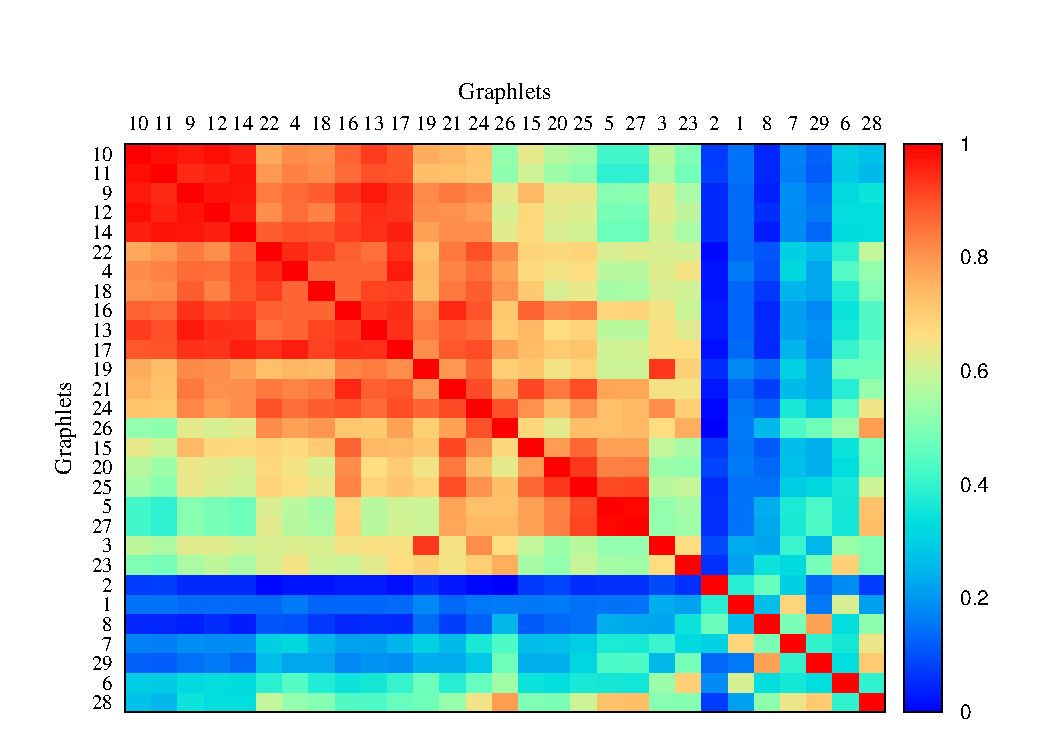
\includegraphics[scale=1.0]{../code/final_results_norm1/trade_2010_thresholded/heatmap_pearsons_hclust_trade_2010_thresholded2.pdf}}
  \caption[Pearson's GCV correlation matrix for the 2010 WTN using the normalised GCV]{Pearson's GCV correlation matrix for the 2010 WTN using the normalised GCV. The heat map is normalised only with feature scaling.}
  \label{fig:trade_norm1}
\end{figure}


% can also use \item[\textbf{A}]
Figure \ref{fig:trade_norm1} shows the Pearson's correlation matrix on the 2010 WTN that is calculated using the normalised GCV signature. We can observe several clusters of graphlets that have been formed along the diagonal:
\begin{itemize}
 \item \textbf{A}: Cluster made of graphlets \{10,11,9,12,14\}. These are all sparse graphlets that have 4 or 5 nodes.
 \item \textbf{B}: A slightly similar cluster that is also correlated with the one above is \{22,4,18,16,13,17\}. These graphlets all contain a $C_4$ as a subgraph.
 \item \textbf{C}: Another cluster is formed by graphlets \{5,25,27\}. These graphlets all contain a cycle of length 4 ($S_4$).  
\end{itemize}

However, we also notice that this time the cliques \{2,8,29\} do not cluster together. Cliques used to cluster together when using the un-normalised GCV signature (see figure \ref{fig:trade_heatmap}). We do not have a clear explanation for this behaviour and further research needs to be done into this. 

\subsection{Normalised GCV - Canonical Correlation Analysis}
\label{cca_trade_norm1}

After finding out which graphlets cluster together, we run Canonical Correlation Analysis using the same methodology described in section \ref{sec:cca_orig}, this time using the normalised GCV signature. Figure \ref{fig:all_trade_cca_black} shows the results of the CCA, while the supplementary table with all the correlations can be found in the appendix figure \ref{all_trade_thresh_cca}. The correlation is high $\rho = 0.94$ and the p-value is 0.0, suggesting that the result is statistically significant. 



% \rowcolors{1}{}

%                           red        green
% \definecolor{cca73p}{rgb}{0.13,0.87,0} % med blue
% \definecolor{cca29p}{rgb}{0.35,0.65,0} % med blue
% \definecolor{cca10n}{rgb}{0.55,0.45,0} % med blue
% % \definecolor{cca-26}{rgb}{1+0.26,0.29,0} % med blue
% 
% \definecolor{cca80n}{rgb}{0.90,0.10,0}



\newcommand{\ccaIndicatorsTradeNorm}{
  \begin{tabular}{r}
  \cellcolor{black}\textcolor{ccacol1}{POP}\\
  \cellcolor{black}\textcolor{ccacol1}{LE}\\
  \cellcolor{black}\textcolor{ccacol2}{KI}\\
  \cellcolor{black}\textcolor{ccacol2}{RGDPCH x POP}\\
  \cellcolor{black}\textcolor{ccacol2}{RGDPL x POP}\\
  \cellcolor{black}\textcolor{ccacol2}{RGDPL2 x POP}\\
  \cellcolor{black}\textcolor{ccacol2}{KG x RGDPL x POP}\\
  \cellcolor{black}\textcolor{ccacol2}{KC x RGDPL x POP}\\
  \cellcolor{black}\textcolor{ccacol3}{KC x RGDPL}\\
  \cellcolor{black}\textcolor{ccacol4}{XRAT}\\
  \cellcolor{black}\textcolor{ccacol4}{RGDPCH}\\
  \cellcolor{black}\textcolor{ccacol4}{RGDPL}\\
  \cellcolor{black}\textcolor{ccacol4}{RGDPL2}\\
  \cellcolor{black}\textcolor{ccacol4}{KG x RGDPL}\\
  \cellcolor{black}\textcolor{ccacol4}{KI x RGDPL}\\
  \cellcolor{black}\textcolor{ccacol4}{KC}\\
  \cellcolor{black}\textcolor{ccacol5}{KI}\\
  \cellcolor{black}\textcolor{ccacol5}{BCA per RGDPL}\\
  \cellcolor{black}\textcolor{ccacol5}{KG}\\
  \cellcolor{black}\textcolor{ccacol5}{BCA}\\
  \cellcolor{black}\textcolor{ccacol6}{OPENK}
  \end{tabular}

}


\begin{figure}[H]
  \centering
    \begin{tikzpicture}[scale=\ccafigscale,show background rectangle, 
  background rectangle/.style={fill=black},
  color=white,help lines/.style={color=lightgray,line width=0.2pt},post/.style={->,shorten >=1pt,>=stealth',thick}]

    \node[upper left,inner sep=0,scale=\ccafigscale] (indicators) at (-2.0,0) {\ccaIndicatorsTradeNorm};	
    \shade[top color=green,bottom color=yellow] (4,0) rectangle (4.5,5);
    \shade[top color=yellow,bottom color=red] (4,-5) rectangle (4.5,0);
    \node[upper left,inner sep=0] (dummy) at (13.0,4) {}; % for extending the black bounding box
    \node[upper left,inner sep=0] (corr_text) at (4.25,-6.0) {Correlation};
    \node[upper left,inner sep=0,red] (corr_text) at (4.25,-5.5) {-1};
    \node[upper left,inner sep=0, green] (corr_text) at (4.25,5.5) {1};
    \node[upper left,inner sep=0] (corr_text) at (4.75,0) {0};
    
    \node[upper left,inner sep=0,scale=\ccafigscale] (g12) at (7.5,4.0) {\gtwelvecca{ccacol1}};
    \node[upper left,inner sep=0,scale=\ccafigscale] (g10) at (10.5,2.5) {\gtencca{ccacol1}};
    \node[upper left,inner sep=0,scale=\ccafigscale] (g14) at (7.5,1.0) {\gfourteencca{ccacol1}};
    \node[upper left,inner sep=0,scale=\ccafigscale] (g2) at (10.5,-1.0) {\gtwocca{ccacol8}};
    \node[upper left,inner sep=0,scale=\ccafigscale] (g29) at (7.5,-2.5) {\gtwentyninecca{ccacol8}};
    \node[upper left,inner sep=0,scale=\ccafigscale] (g8) at (10.5,-4.0) {\geightcca{ccacol8}};
    
    
%     \draw[line,color=ccacol1] (0,4.8) -| (3,5) -- (4.25,5); % top-left elem
%     \draw[line,color=ccacol1] (0,4.35) -| (2,3.9) -- (4.25,3.9); % next in line
    
    \draw[line,color=ccacol1] (0.00,4.80) -| (1.75,3.68) -- (4.00,3.68);
    \draw[line,color=ccacol1] (0.00,4.33) -| (1.49,3.58) -- (4.00,3.58);
    \draw[line,color=ccacol1] (0.00,3.85) -| (1.37,3.30) -- (4.00,3.30);
    \draw[line,color=ccacol1] (0.00,3.38) -| (1.07,3.27) -- (4.00,3.27);
    \draw[line,color=ccacol1] (0.00,2.90) -| (1.25,3.27) -- (4.00,3.27);
    \draw[line,color=ccacol1] (0.00,2.42) -| (1.56,3.26) -- (4.00,3.26);
    \draw[line,color=ccacol1] (0.00,1.95) -| (1.84,3.21) -- (4.00,3.21);
    \draw[line,color=ccacol1] (0.00,1.48) -| (2.13,3.17) -- (4.00,3.17);
    \draw[line,color=ccacol3] (0.00,1.00) -| (1.31,1.46) -- (4.00,1.46);
    \draw[line,color=ccacol4] (0.00,0.53) -| (1.22,0.85) -- (4.00,0.85);
    \draw[line,color=ccacol4] (0.00,0.05) -| (1.50,0.80) -- (4.00,0.80);
    \draw[line,color=ccacol4] (0.00,-0.42) -| (1.82,0.80) -- (4.00,0.80);
    \draw[line,color=ccacol4] (0.00,-0.90) -| (2.13,0.80) -- (4.00,0.80);
    \draw[line,color=ccacol4] (0.00,-1.38) -| (2.30,0.79) -- (4.00,0.79);
    \draw[line,color=ccacol4] (0.00,-1.85) -| (2.58,0.52) -- (4.00,0.52);
    \draw[line,color=ccacol4] (0.00,-2.33) -| (2.68,0.43) -- (4.00,0.43);
    \draw[line,color=ccacol5] (0.00,-2.80) -| (2.77,-0.08) -- (4.00,-0.08);
    \draw[line,color=ccacol5] (0.00,-3.27) -| (2.92,-0.55) -- (4.00,-0.55);
    \draw[line,color=ccacol5] (0.00,-3.75) -| (3.07,-0.64) -- (4.00,-0.64);
    \draw[line,color=ccacol5] (0.00,-4.23) -| (3.32,-0.75) -- (4.00,-0.75);
    \draw[line,color=ccacol6] (0.00,-4.70) -| (3.55,-1.33) -- (4.00,-1.33);

    
    
    \draw[line,color=ccacol1] (g12) -| (5.5,4.5) -- (4.5,4.5);
    \draw[line,color=ccacol1] (g10) -| (5.3,4.47) -- (4.5,4.47);
    \draw[line,color=ccacol1] (g14) -| (5.1,4.43) -- (4.5,4.43);

    \draw[line,color=ccacol8] (g2) -| (5.3,-2.5) -- (4.5,-2.5);
    \draw[line,color=ccacol8] (g29) -| (5.5,-3) -- (4.5,-3);
    \draw[line,color=ccacol8] (g8) -| (5.1,-3.5) -- (4.5,-3.5);
    
    \end{tikzpicture}
    \caption[CCA - World Trade networks - normalised GCV - Picture version]{CCA between economic indicators and the normalised GCV signature. Only the graphlets that show the strongest respectively weakest correlations are shown. One can notice that graphlets \{12,10,14\} are relatively sparse, while graphlets \{2,29,8\} are dense, being cliques. The sparse graphlets are correlated with the good economic indicators (in green) such as Population (POP), Level of Employment (LE) and GDP per Capita (RGDPL), while dense graphlets are correlated with bad indicators (in red) such as the Balance of Current Account (BCA). The canonical correlation $\rho = 0.94$ and the p-value is smaller than 0.0001, suggesting that the result is statistically significant.}
    \label{fig:all_trade_cca_black}	
\end{figure}


The good indicators such as population (POP), level of employment (LE) and GDP per capita (RGDPL) are positively correlated with the graphlets \{12,10,14,17,9, \dots \}\footnote{The CCA figure \ref{fig:all_trade_cca_black} only shows the graphlets that have the strongest and weakest cross-loadings. See figure \ref{all_trade_thresh_cca} in the appendix for a list of cross-loadings for all the graphlets and economic indicators.}. On the other hand, the bad indicators such as the balance of current account (BCA) correlate positively with graphlets \{8,29,2,7,1,28\}. Graphlets \{10,12,14,9\} on the positive side of the spectrum have also clustered together in the Pearson's correlation matrix (section \ref{sec:trade_pears_norm1}). We first notice that graphlets \{8,29,2,7,1,28\} represent cliques \{8,29,2\} or almost cliques \{7,1,28\}. Since these graphlets are very densely connected, this suggests that the trading partners of small and poor countries are trading heavily with each other or form highly connected 
clusters. As a result, we deduce that \emph{the majority of the trading partners of small and poor countries are the big and rich countries that are always trading heavily with each other}. 

This theory seems to be confirmed by taking a few small and poor countries and looking at their trading partners. Note that since the network has only 119 countries, the poorest countries from Africa or South Asia have already been filtered out.\footnote{This is the case because the network has been thresholded at an 85\% level. See section \ref{sec:trade_bck} for more details.} Therefore, let us consider Morocco a small and poor country relative to the others, although in reality it considered to have a medium level of development. Morocco's main trading partners are: Saudi Arabia, China, France, USA, Spain, Germany and Italy. These countries are big and rich and every single pair of them clearly trade with each other. Similar results have been observed for other countries such as Uruguay. Moreover, all of Morocco's trading partners are part of G20, a club of big and wealthy countries that collaborate with each other on economic matters. This leads us to a second theory: \emph{since the trading 
partners of a small and poor country form highly connected clusters, these clusters represent big and rich economic groups such as G8, G20, OECD\footnote{Organisation for Economic Co-operation and Development} or Paris-club\footnote{A group of countries that provide debt relief and debt restructuring to indebted countries and their creditors.}}. This theory can be validated by selecting a few countries and looking at their neighbours. For example, the biggest trading partners of Tunisia are Germany, France and Italy, all part of G8, G20, OECD and Paris-club. 

Regarding the first group of graphlets (i.e.\ \{12,10,14, \dots \}), we notice that all of them are sparse graphlets that contain relatively few edges. Having the sparse graphlets at one end of the spectrum and the dense graphlets at the other suggests that the graphlets are roughly ordered according to their density. Therefore, CCA shows that the sparse graphlets correlate with the good indicators such as population (POP), level of employment (LE) and GDP per capita (RGDPL) while dense graphlets correlate with bad indicators such as the balance of current account (BCA).

Now that we now know to interpret the positively weighted part of the graphlet vector as sparse graphlets, canonical correlation tells us that the trading partners of big and wealthy countries have a lot of sparse graphlets in their neighbourhood. The economic reason for this is because \emph{big and rich countries like USA, China, Russia are trading with a lot of small, isolated countries which in turn do not trade with each other}. This theory is supported by a closer analysis with Cytoscape\footnote{A network analysis software that can provide useful statistics of the network data.}. Using this software we found that the clustering coefficient of a country is inversely correlated with the wealth and size of that country, suggesting that big and rich countries indeed have a relatively sparse neighbourhood.


\subsection{Normalised GCV - Correlation matrix change during 1962--2010}
\label{rev_trade_change}

% Put them when the report is ready
% gcv offset: -1   Spearman's rank coefficient: corr: 0.340675635498    p_value: 0.0191171684701

We also calculated the changes in Pearson's correlation matrix using the normalised GCV for the WTNs over the period 1962--2010. The results are plotted in figure \ref{change_over_time_norm1} along with the changes in Crude Oil price. For this experiment we follow the same methodology as in section \ref{trade_change_orig}. We find that for the normalised GCV, the best results are obtained when the GCV vector is shifted with -1 year and yields a positive correlation $\rho = 0.34$ and a p-value of $p = 0.01$. These results are in contrast to the ones obtained using the original GCV signature in section \ref{trade_change_orig} and at the moment we cannot give a reason why this is happening. Since the best correlation is obtained when the GCV vector is shifted with -1, this again suggests that the changes in the network structure might cause the changes in the price of Crude Oil.

\begin{figure}[H]
  \centering
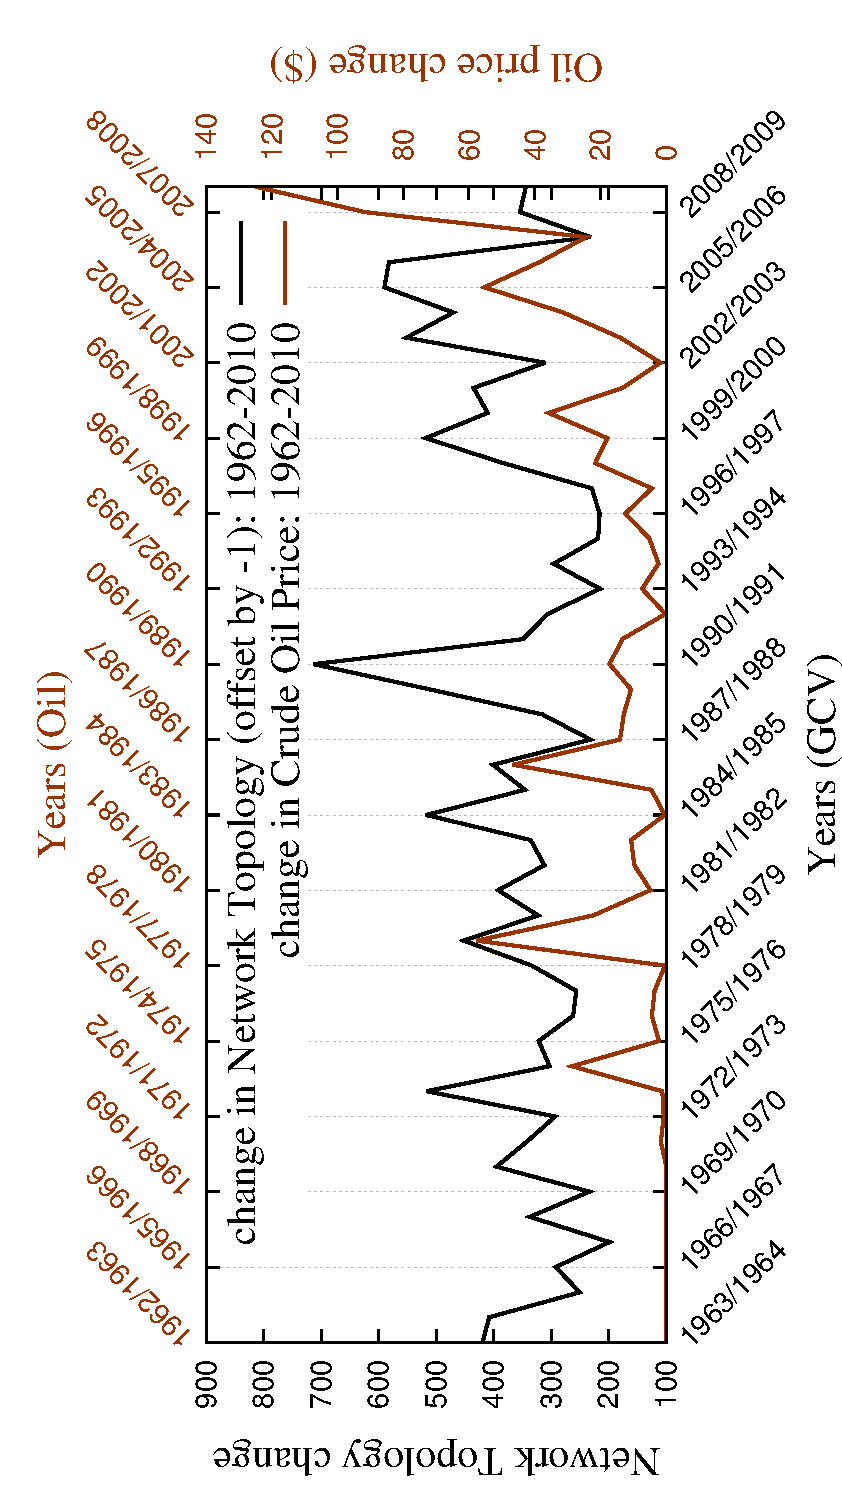
\includegraphics[angle=-90,scale=0.6]{../code/final_results_norm1/all_trade_thresh/change_over_time2}
\caption[Change in WTN topology - normalised GCV]{Change in WTN topology (as measured by the normalised GCV correlation matrix) versus change in crude oil price. The two plots are positively correlated, having a Spearman's rank correlation coefficient of 0.34 and p-value of 0.01. The best correlation coefficient is obtained when the change in network topology is shifted by -1 years. The top and left axis tics correspond to the Oil curve, while the bottom and the left axis tics correspond to the network topology curve.}
\label{change_over_time_norm1}
\end{figure}

There are several major economic and social events that have clearly affected the WTN structure. The 1970s were marked by two energy crises (1973 and 1979) that explain the two small peaks in both the topology change but also in the oil price change. Afterwards, the 1983/1984 peak in network topology change might have been caused by the early 1980s recession, which affected most of the developed world. A revival of neoliberalist economic policies around the world occurred in this period which led to reduced government intervention, lower taxes and deregulation. The peak in 1989 might be explained by the fall of communist/socialist governments in Russia, Eastern Europe and around the world accompanied by a fall in heavy industries and increased trade openness. These events have been accompanied by changes in government for some former left-wing or right-wing countries such as Russia, Poland, Chile and South Africa.

The early 1990s appear as a period of relatively low changes in oil and network topology, which reflects the overall economic stability at that time. However, bigger changes are noticed in the late 1990s, possibly started by the 1997 Asian financial crisis. By the 2000s, even bigger changes can be observed in the network topology plot that were caused by the commodities boom and rising oil prices and inflation. 

\subsection{Trade partners sparsity index}
\label{sec:sparsity_index}

Using a combination of graphlet frequencies that are part of the GCV, we are now interested to create an index that is positively correlated with the good indicators from section \ref{cca_trade_norm1} such as GDP per Capita (RGDPL) or Level of Employment (LE). Therefore, we take the three graphlets that have the highest correlation with the economic indicators variate \{12,10,14\} and the three that have the lowest correlation \{8,29,2\} (see figure \ref{all_trade_thresh_cca}). Multiplying each of these by their respective CCA cross-loading and summing up the results gives us a \emph{trading partner sparsity index}. The index $T$ can formally be defined as:

$$ T = w_{12}F_{12} + w_{10}F_{10} + w_{14}F_{14} + w_{8}F_{8} + w_{29}F_{29} + w_{2}F_{2}$$
where $F_i$, $w_i$ are the frequency respectively the canonical cross-loading of $G_i$. In order to compute the index, we use the cross-loadings obtained from CCA in figure \ref{all_trade_thresh_cca}.

This index can be calculated for every country and for every year and can have both positive and negative values. It gives a measure of the sparsity of the network of the trading partners: the higher the value the sparser the neighbourhood, because the sparse graphlets have positive weights while the dense graphlets have negative weights. CCA has shown us that for a certain country a network of trading partners that 
has sparse graphlets indicates a healthy economy, so we expect the \emph{trading partner sparsity index} to be high for big and wealthy countries and low for small and poor countries. We also expect the index to fluctuate during periods of economic uncertainty.

\begin{figure}[H]
  \centering
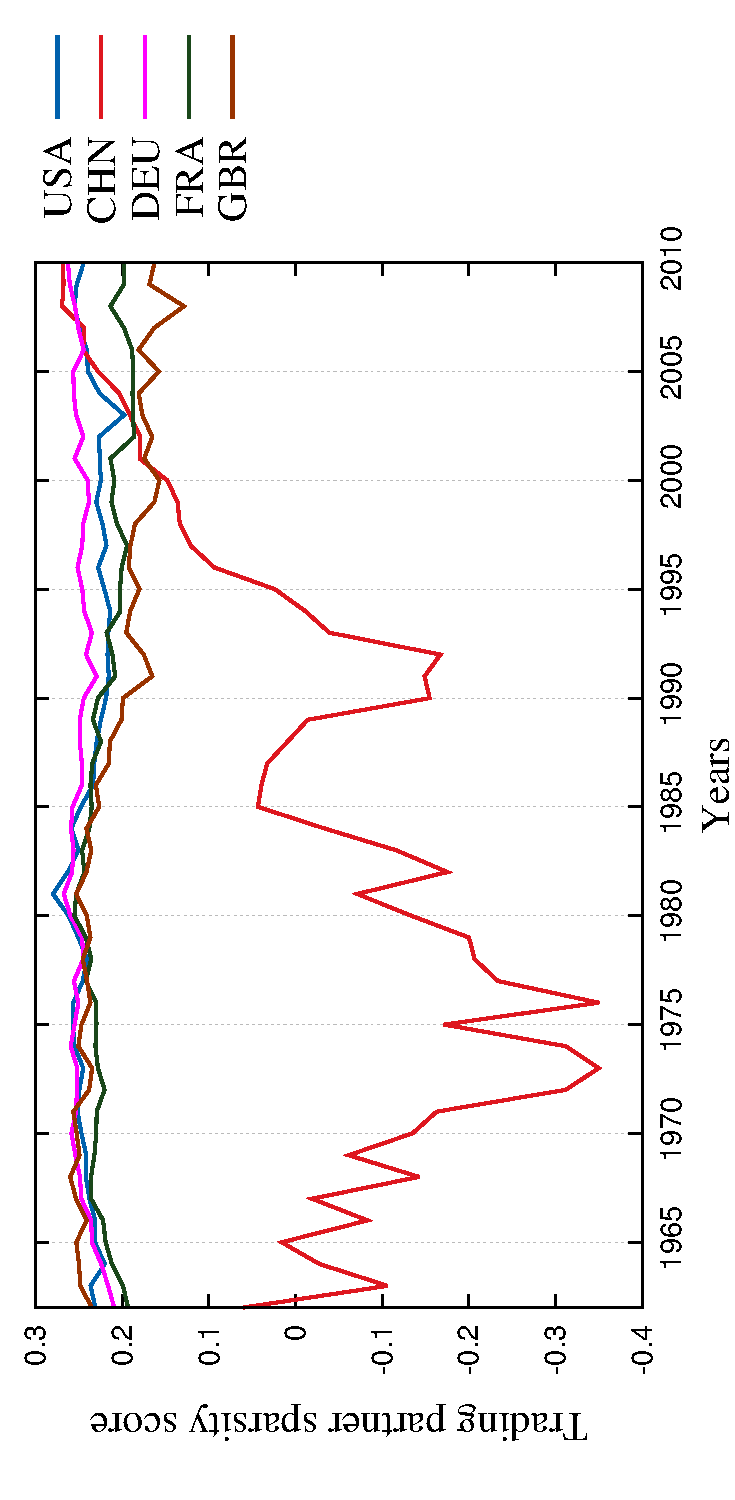
\includegraphics[angle=-90,scale=0.6]{../code/extra_results/trading_partner_density/scores/g72.pdf}
\caption[Trading partners sparsity index -- United States (USA), China (CHN), Germany (DEU), France(FRA) and the United Kingdom (GBR)]{Trading partners sparsity index measured for 5 big economies: United States (USA), China (CHN), Germany (DEU), France(FRA) and the United Kingdom (GBR). The index for US, Germany, France and the UK is approximately flat over the 49-year period. However, the index of China has a downward trend over the time period 1963--1973 due to Mao Zedong's policies that harmed the economy of the country. However, the period after 1975 shows a surge that was boosted by economic reforms and growth. There is one exception in 1990--1992 right after the Fall of Communism in Eastern Europe, a global event that affected a socialist country such as China.}
\label{g7_sparsity_index}
\end{figure}

Figure \ref{g7_sparsity_index} shows the \emph{trading partners sparsity index} for several influential countries: United States (USA), China (CHN), Germany (DEU), France(FRA) and the United Kingdom (GBR). Throughout the 1965--2010 period, the corresponding index for the United States, Germany, France and the United Kingdom has been approximately flat, having a value of 0.2. Some small variation can be seen starting from 1990, with Germany and the United States having a slightly bigger index than France and the United Kingdom. Furthermore, for these four countries we don't observe any shocks during economic crises. On the other hand, China suffers a decrease in the trading partners sparsity index during 1965--1976, due to Mao Zedong's Cultural Revolution that resulted in a period of economic decline. However, the index increases again during 1976--1985, probably due to economic reforms that were initiated by Deng Xiaoping which helped revive the economy. Another low point is noticed in 1990--1992 right at 
the Fall of Communism in USSR and Eastern Europe, a global event that deeply affected a socialist state such as China.

\begin{figure}[H]
  \centering
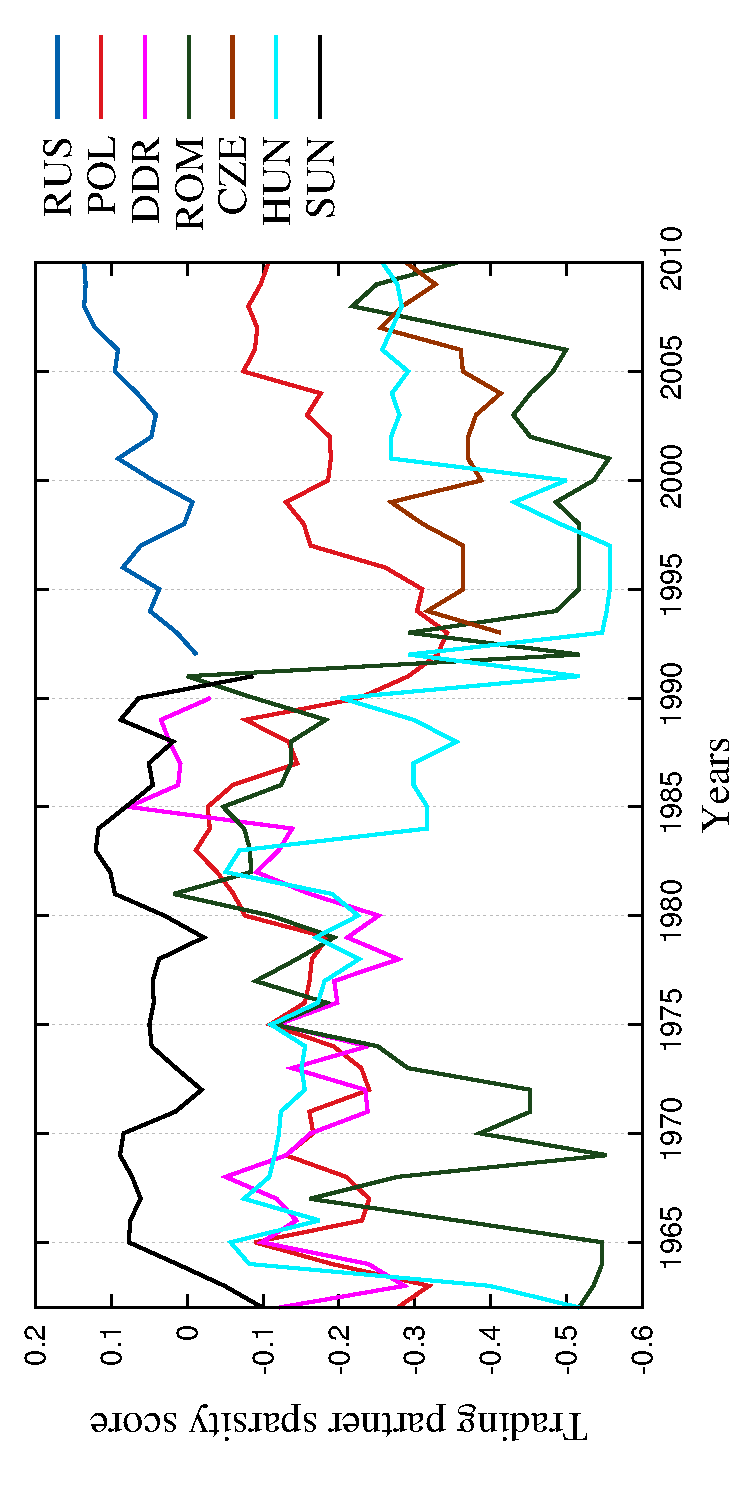
\includegraphics[angle=-90,scale=0.6]{../code/extra_results/trading_partner_density/scores/eastern_europe2.pdf}
\caption[Trading partners sparsity index -- Russia (RUS), Poland (POL), East Germany (DDR), Romania (ROM), Czech Republic (CZE), Hungary (HUN) and the USSR (SUN)]{Trading partners sparsity index measured for countries from Eastern Europe: Russia (RUS), Poland (POL), East Germany (DDR), Romania (ROM), Czech Republic (CZE), Hungary (HUN) and the USSR (SUN). Most of the countries show a drop in the index after 1990 because of the Fall of Communism and the economic restructuring that took place at that time.}
\label{eastern_europe_sparsity_index}
\end{figure}

Figure \ref{eastern_europe_sparsity_index} shows the \emph{trading partners sparsity index} for several countries in Eastern Europe: Russia (RUS), Poland (POL), East Germany (DDR), Romania (ROM), Czech Republic (CZE), Hungary (HUN) and the USSR (SUN). In the period leading to 1990, the USSR had the highest index since it was a world superpower, while it's satellite states had a lower index. However, the Revolutions in December 1989 in Eastern Europe led to a large drop in the \emph{trading partners sparsity index} for all these countries, a fact that is reflected by the economic situation at that time: unemployment skyrocketed and living standards fell considerably. It took some countries such as Poland of Hungary around approximately 10--15 years to reach the pre-revolutions level in the \emph{trading partners sparsity index}.

\begin{figure}[H]
  \centering
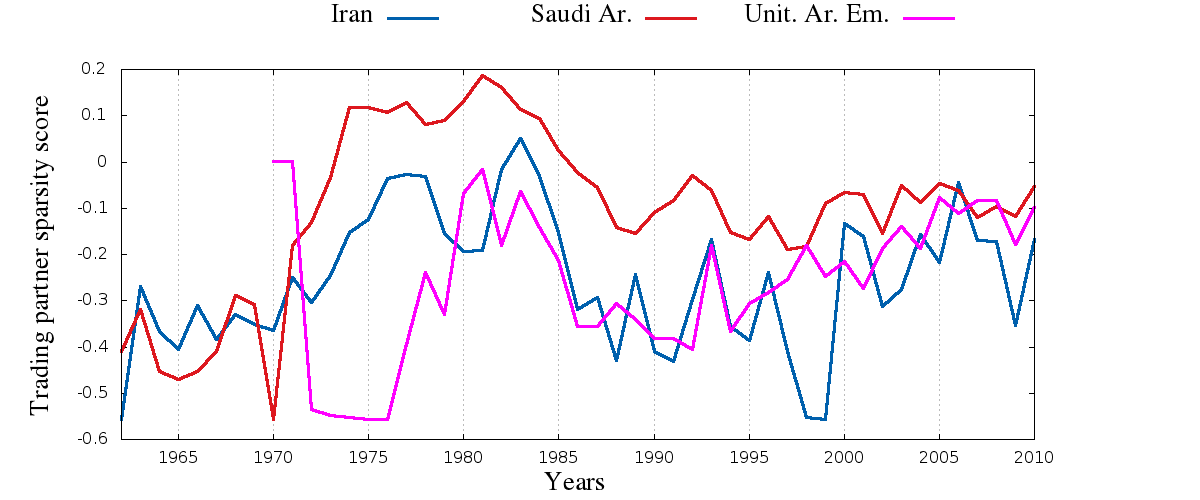
\includegraphics[angle=-90,scale=0.6]
{../code/extra_results/trading_partner_density/scores/opec2}
\caption[Trading partners sparsity index -- Iran (IRN), Saudi Arabia (SAU) and United Arab Emirates (ARE)]{Trading partners sparsity index measured for 3 OPEC members: Iran (IRN), Saudi Arabia (SAU) and United Arab Emirates (ARE). The rise in petroleum prices and the Oil crisis in 1973 has led to a surge in the index for Saudi Arabia and Iran. Moreover, the Oil crisis of 1979 has also led to an increase in United Arab Emirate's index. However, the 1980s Oil glut that was caused by a serious surplus of oil had detrimental effects on all OPEC members, which is reflected in the drop of their trading partners density index.}
\label{opec_sparsity_index}
\end{figure}

Figure \ref{opec_sparsity_index} shows the \emph{trading partners sparsity index} for three main OPEC members: Iran, Saudi Arabia and United Arab Emirates. For Saudi Arabia and Iran, the rise in petroleum prices in 1970s led to a surge in it's index. However, during the 1980s the oil glut that was caused by a serious surplus of crude oil and a drop in demand had detrimental effects on all OPEC members, which are heavily dependent on the price of oil. It can also be noticed that the 1973 Oil Crisis has led to an increase in the index only for Saudi Arabia and Iran, while the 1979 Oil crisis has led to an increase in the index only for the United Arab Emirates.

\subsection{Case study: Saudi Arabia}
\label{case_study_saudi}
% norm1 GCV vector results

%gcv offset: -1   Spearman's rank coefficient: corr: -0.323529495316    p_value: 0.0265331450245
% offset 1 gives the best results .. tried [-2,-1,0,1,2]

% orig GCV results are all bad, even if offset by +- 0-2 years

As we have seen in previous sections, the GCV signature can indeed capture the changes in Crude Oil prices and correlate with key economic and social events around the world. In this section we are trying to apply the same analysis but on a smaller scale, at a country level. We have selected Saudi Arabia as a major oil-exporting country, whose economy is heavily dependent on the price of oil. We are trying to find the answer to the following questions:
\begin{itemize}
 \item Are the partners of Saudi Arabia affected by changes in Crude Oil price?
 \item Is the GCV of Saudi Arabia positively or negatively correlated with the Crude Oil Price?
\end{itemize}

Saudi Arabia is the world's largest oil-exporting economy and has the largest proven petroleum reserves. It is also a very influential member of the \emph{Organisation of the Petroleum Exporting Countries} (OPEC). It's main export partners are the United States, China and Japan, while it's main import partners are China, United States and South Korea. Around 90\% of it's exports consist of petroleum and related products. 

We therefore calculate the normalised GCV of Saudi Arabia for each year in the period 1962--2009. Afterwards, the change in GCV between every two consecutive years is calculated using the Euclidean distance between the two vectors. Results of the GCV change along with the Crude Oil price are plotted in figure \ref{saudi_oil}. The two plots are negatively correlated, having a Spearman's rank correlation coefficient of -0.32 with a p-value of 0.026, which resembles the results we got for the original GCV change for the overall trade network in section \ref{trade_change_orig}. First of all, it must be noted that since Saudi Arabia is an oil-exporting country, it benefits massively from a rise in oil prices. However, high oil prices on the energy markets lead to less demand for petrol and provides other oil-poor countries an incentive for developing alternative sources of energy. The fact that Saudi Arabia benefits from high oil prices might explain why the change in it's trading partner network topology is 
inversely correlated with oil price: when the price of oil is low, Saudi Arabia always looks for new export markets and thus has a move volatile network of trading partners. On the other hand, when the price of oil is high, it means that the demand is much higher than the supply available, so Saudi Arabian oil companies prefer to export to their old trading partners, since there is no need for extra contracts, negotiations and bureaucracy.

Figure \ref{saudi_oil} shows that big changes in the trading partners of Saudi Arabia occurred between 1968/1969 and 1969/1970, which subsumed shortly afterwards. These might be explained as a consequence of the 1967 Oil Embargo, when Saudi Arabia and several Middle Eastern countries limited or completely stopped their oil supplies to Western countries such as the USA, UK and other European states. The result was that Saudi Arabia had to look for different export partners and that led to a change in its trading partner structure.

This experiment has also been run using the un-normalised GCV change, but it hasn't yielded a good correlation between the GCV change and the change in crude oil price. The associated p-value was also high, meaning that the result was not statistically significant. A plot and the equivalent results are given in figure \ref{saudi_oil_orig} in the appendix.

\begin{figure}[H]
  \centering
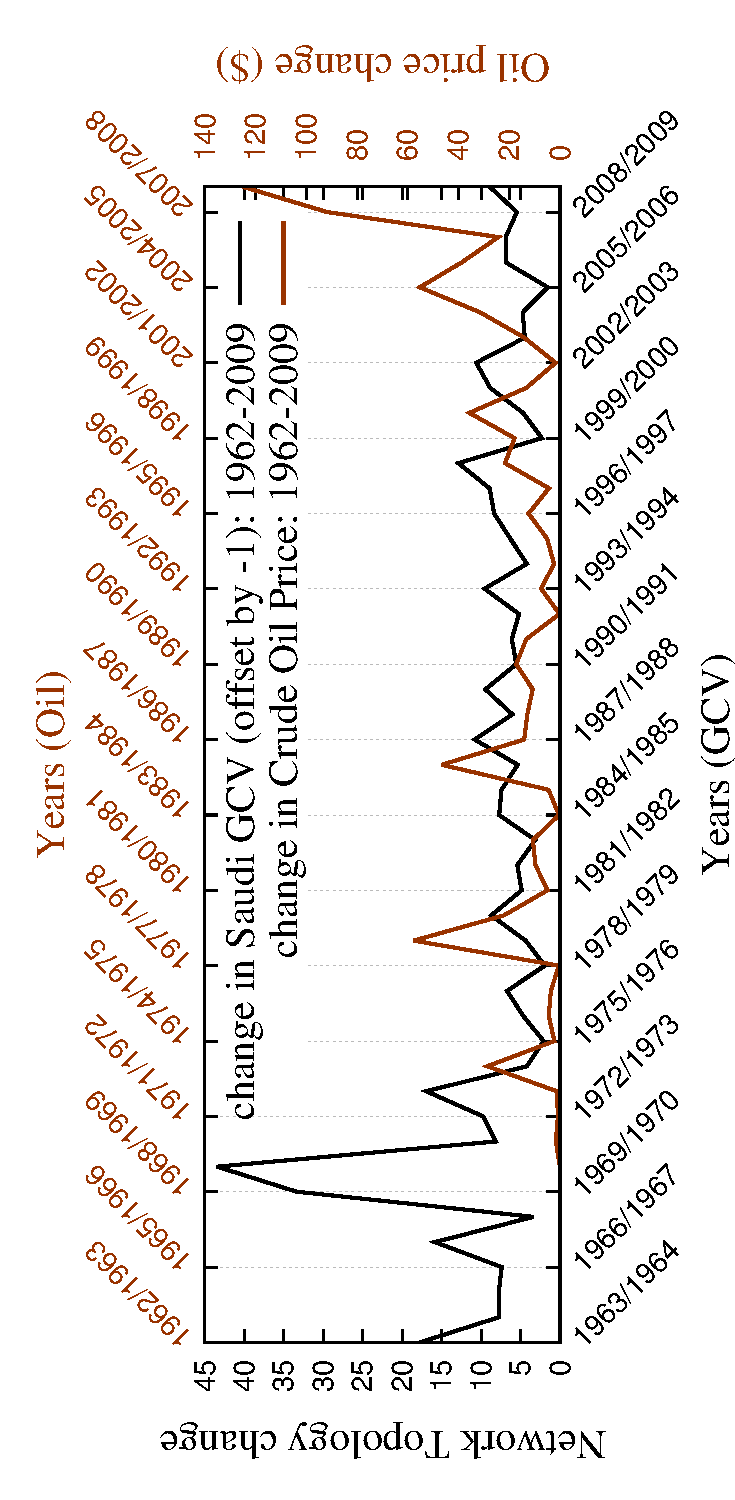
\includegraphics[angle=-90,scale=0.6]
{../code/extra_results/saudi_oil/saudi_norm1_gcv_oil2}
\caption[The change in the GCV of Saudi Arabia along with the change in Crude Oil price.]{The change in the GCV of Saudi Arabia along with the change in Crude Oil price. The two plots are negatively correlated, having a Spearman's rank correlation coefficient of -0.32 with a p-value of 0.026. This correlation is obtained when the vector of changes in Saudi GCV is shifted by -1. Top and left axis tics correspond to the Oil curve, while the bottom and the right axis tics correspond to the Saudi GCV curve.}
\label{saudi_oil}
\end{figure}


%cca_oil/CCA_out/saudi_oil.txt

In order to find out how each of the individual elements of the GCV vector are influenced by the oil price, we apply Canonical Correlation between the GCV of Saudi Arabia and the Crude Oil price index. However, this proves to be problematic since we only have 49 samples to run the CCA on, one for every year during 1962--2010\footnote{In previous CCA experiments, we used all country-year pairs that gave us in total around $119 * 29 = 3451$ samples, where $119$ is the average number of countries in the network and $29$ is the number of years CCA was run on (period 1980-2010). The reason CCA was run from 1980 is because we did not have data for the economic indicators prior to 1980.}. On the other hand, there are $29 (\text{GCV}) + 1(\text{Oil Price}) = 30$ parameters that need to be estimated. This could easily overfit or yield singularities in our algorithm. Therefore, we trim down the GCV vector to only contain the essential graphlets 1-8, discarding all the 5-node graphlets. The final CCA variates  are as 
follows:
\begin{itemize}
 \item[X] - short 8-element GCV of Saudi Arabia that only contains the essential graphlets (i.e.\ $G_1-G_8$)
 \item[Y] - a single-element vector containing the Oil price 
\end{itemize}

Results for the CCA analysis are shown in figure \ref{saudi_oil_cca}. It is shown that graphlet $G_3$ correlates positively with the increase in Oil price, while graphlets \{1,2,8\} correlate negatively. One property that separates the two ends of the graphlet spectrum is their density. Graphlet $G_3$ is a sparse graphlet, while graphlets \{1,2,8\} are dense graphlets having a density of at least 0.66. 

Using the results we got earlier from section \ref{cca_trade_norm1}, we know that sparse graphlets correlate with good economic indicators such as GDP per Capita (RGDPL), while dense graphlets correlate with bad economic indicators such as Balance of Current Account (BCA). Using this observation and the fact that sparse graphlets correlate positively with the oil price and dense graphlets vice versa, we can conclude that for Saudi Arabia the good economic indicators such as GDP per Capita, a result of a healthy economy, must correlate with the Oil price\footnote{if the correlation of XY is strictly positive and the correlation of YZ is likewise, then the correlation of X and Z is not necessarily strictly positive. This is however the case if the correlations of XY respectively YZ are close to 1 \cite{langford2001property}.}. This is confirmed by the fact that Saudi Arabia is an Oil-exporting economy, and it's GDP per Capita has been shown to strongly correlate with the Oil price \cite{
lescaroux2008influence}. We expect similar behaviour for other oil-exporting economies such as Libya, Venezuela, Qatar or Russia.

\begin{figure}[H]
\centering
\begin{tabular}{ c c | c c }
  \multicolumn{2}{c}{Canonical Correlation} &  \multicolumn{2}{c}{0.82353} \\
  \multicolumn{2}{c}{p-value} &  \multicolumn{2}{c}{0.00000} \\
  \hline
  \multicolumn{2}{c}{X variate} & \multicolumn{2}{c}{Y variate}\\
  \hline
 G3 & 0.49265 &  Crude Oil price & 0.83032\\
 G6 & 0.09838 &  & \\
 G4 & 0.05294 &  & \\
 G5 & 0.03942 &  & \\
 G7 & -0.23884 &  & \\
 G8 & -0.46603 &  & \\
 G2 & -0.50725 &  & \\
 G1 & -0.52241 &  & \\
\end{tabular}
\caption[Canonical Correlation Analysis between the short GCV vector of Saudi Arabia and the price of Crude Oil.]{Canonical Correlation Analysis between the short GCV vector of Saudi Arabia and the price of Crude Oil. Only the short GCV-8 vector has been used because of the lack of samples. The results show that graphlet $G_3$ is has a strong positive correlation with the price of Crude Oil, while graphlets \{1,2,8,7\} have a negative correlation. This suggests that when the price of Oil is high, the trading partners of Saudi Arabia tend to form paths of 4 nodes ($P_4$). On the other hand, when the price of Oil is low, the trading partner network of Saudi Arabia tends to cluster (\{1,2,8,7\} are dense graphlets with a density of at least 0.66). This might be explained by the fact that when the price of Oil is high, Saudi Arabia starts new trading partnerships with isolated countries that are not part of a clustered network.}
\label{saudi_oil_cca}
\end{figure}


\section{Protein-protein Interaction Networks}
\label{ppi_res_heatmaps}

In this section we apply our methodology for various PPI Networks. For more background information about how these networks are built and their properties, see section \ref{sec:ppi_bck}. We now present the Pearson's correlation matrix for a Human PPI network and Canonical Correlation Analysis results for six different Human and Yeast PPI networks using two annotation files: Boone's and von Mering's (see annotation descriptions in section \ref{sec:ppi_bck}). In short, the heat map of the Pearson's GCV correlation matrix did not give us any useful information, since graphlets formed faint clusters. However, the CCA results have helped us get some interesting insights into the interactions of the proteins present in these networks. 

\subsection{Analysis of Pearson's GCV Correlation Matrix}

\begin{figure}
  \centering
  \hbox{\hspace{-1cm}
  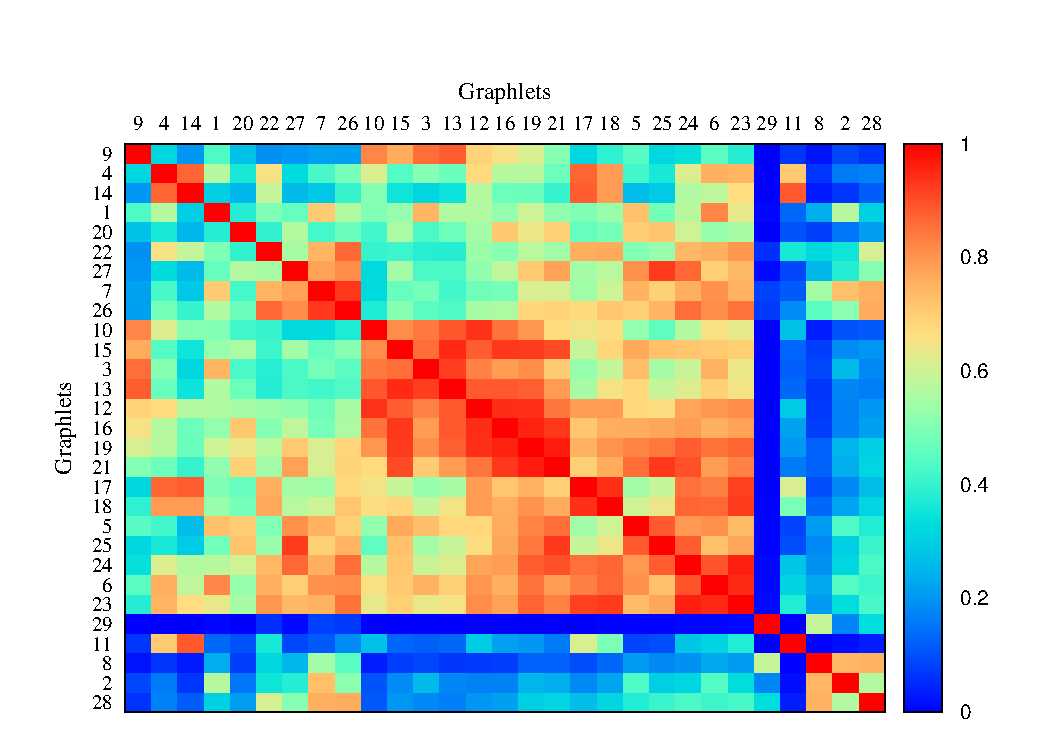
\includegraphics[scale=1.0]
  {../code/final_results/human_ppi/heatmap_pearsons_hclust_human_ppi-poly-42.pdf}}
  \caption[Heat map for the Pearson's GCV correlation matrix of the Human PPI network]{Heat map for the Pearson's GCV correlation matrix of the Human PPI network. The heat map has been first normalised with feature scaling and a $4^{th}$ degree polynomial and then hierarchically clustered.}
  \label{fig:human_ppi}
\end{figure}



The heat map from figure \ref{fig:human_ppi} represents the Pearsons's correlation heat map for the Human PPI 
network. It was first normalised with a simple feature scaling and then with a $4^{th}$ degree polynomial\footnote{Other polynomial functions have also been tested, but the $4^{th}$ degree polynomial offers the best results.}, because the original correlation matrix yielded correlations that were too strong\footnote{Having all correlations close to 1 made the identification of clusters impossible}. There are a few faint clusters formed on the diagonal:
\begin{itemize}
 \item \{10,15,3,13,12,16,19 and 21\}. These graphlets all contain a $P_4$\footnote{Path on 4 nodes, graphlet $G_3$}.  
 \item \{7,26\} contain a $G_7$.
 \item \{4,14\} contain a $G_4$.
 \item \{17,18\} contain 2 $G_2$'s (triangles).
 \item \{5,25\} contain a $G_5$.
 \item \{24,6,23\} contain a $G_6$.
\end{itemize}

The lack of clear graphlet clusters in the Human PPI is something that we cannot 
explain at the current time. Because of this, it has not been possible for us to get any actual insights from the Human PPI correlation matrix. Other human and yeast PPI networks have yielded similar results. Further research needs to be done into this area in order to explain the lack of graphlet clustering.

\subsection{Canonical Correlation Analysis}


The next step after the Pearson's GCV correlation matrix is to run CCA on the PPI network. We set the $X$ variate to be the GCV and the $Y$ variate to be a vector of values of Boone's annotation. For setting up the $Y$ variate, we label each protein with a vector of binary entries, where the $i^{th}$ entry is as follows:

\rowcolors{1}{}{}
$$ Y_i = \begin{cases} 1, & \mbox{if the protein is annotated with the } i^{th}\mbox{ annotation} \\ 0, & \mbox{otherwise} \end{cases}$$

Since each protein had only one annotation, each sample from $Y$ only contained one non-null entry. The results of the CCA on this network were unfortunately not good, since the correlation is low and the p-value is above 0.05, suggesting that the correlation is not statistically significant. In the next section we will explain the subsequent experiments that have been performed on other PPI networks.

\subsection{Results for other PPI networks}
\label{sec:cca_ppi_intro}

\subsection*{The 17 experiments}


Since the CCA applied to the Human PPI network didn't give us any meaningful information, we thought of exhaustively running it on several types of Human and Yeast PPI networks. We ran the same process on 5 other Human PPI networks with Boone's annotation file and on 6 Yeast networks using the two different annotation files: von Mering's and Boone's (see section \ref{ppi_annotations}). For these experiments we have also used high-confidence networks, which contain only protein interactions that have been confirmed by two independent sources. The networks analysed are as follows:
\begin{itemize}
 \item 5 Human networks
 \begin{itemize}
    \item A high-quality Human PPI network determined by Stitch-seq protocol \cite{yu2011next}, CCA results are not statistically significant.\footnote{In this subsection by statistically significant we mean that either the p-value was above 0.05 or the total correlation was below 0.2}
    \item Two networks from I2D, a database of PPI networks maintained by Jurisca lab \cite{brown2007unequal} at Ontario Cancer Institute:
    \begin{itemize}
      \item Full version, CCA results are not statistically significant.
      \item High-confidence version, CCA results are not statistically significant.
    \end{itemize}
    \item Two networks from BioGRID: 
    \begin{itemize}
      \item Full version, CCA results are not statistically significant.
      \item High-confidence version, CCA results are not statistically significant.
    \end{itemize}
  \end{itemize}
 \item 6 Yeast networks x 2 annotation files
  \begin{itemize}
    \item A network obtained through \emph{affinity-purification mass spectroscopy} (AP-MS) by Collin's et al \cite{collins2007toward} - Co-complex membership associations, CCA results in figures  \ref{yeast_apms_collins_cca}, \ref{all_ppi12}
    \item A genetic network from BioGRID, CCA results in figures   \ref{all_ppi7}, \ref{all_ppi13}
    \item Literature-curated PPI network by Reguly et al. \cite{reguly2006comprehensive}, CCA results are not statistically significant.
    \item Yeast two-hybrid network made from the union of CCSB-YI1, Ito-core and Uetz-screen  \cite{yu2008high}, CCA results are not statistically significant.
    \item Two PPI networks from BioGRID:
    \begin{itemize}
      \item Full version, CCA results in figures  \ref{all_ppi10}, \ref{all_ppi16}
      \item High-confidence version, CCA results in figures   \ref{all_ppi11}, \ref{all_ppi17}
    \end{itemize}
  \end{itemize}
\end{itemize}

The best results have been obtained for the following Yeast networks, for both von Mering's and Boone's annotation files:
  \begin{enumerate}
    \item Collin's AP-MS network
    \item BioGRID Full
    \item BioGRID High-confidence.
  \end{enumerate}

Detailed interpretations of these results are given in the following section. The overall CCA correlations for these networks have been around 0.45-0.5, all having p-values smaller than 0.05. The other combinations of networks and annotation files have yielded much weaker correlations (only approx 0.2) and high p-values above 0.5. Therefore we could not get any insights from the human PPI networks or the other Yeast networks. One of the reason for this might be the amount of noise present in the PPI data. In the next section we present the key Yeast PPI results and provide biological interpretations for the observed phenomena. The other CCA results for all the 17 experiments are shown in the Appendix section 2.

\subsection{Summary of the CCA Results from the 17 experiments}
\label{sec:18_ppi_cca_results}

\subsubsection{Ribosome translation}
% Ribosome translation
Figure \ref{fig:ppi_cca_black} shows the CCA results for Collin's AP-MS\footnote{affinity-purification mass spectroscopy} PPI network. A full list of all the cross-loadings is given in appendix figure \ref{yeast_apms_collins_cca}. The results mainly show that Ribosome Translation is correlated with all the graphlets, since their cross-loadings have the same sign. The spectrum of graphlets runs from the most dense graphlets \{2,8,29\} on top, having the highest cross-loading magnitude of around 1 to the sparser \{9,10,13,11,12\} graphlets at the bottom, having cross-loading magnitudes of approximately 0.46. The observation we can make is the following: \emph{proteins involved in Ribosome translation generally interact more with clusters of other proteins and less with individual proteins}. This result is also confirmed by the same experiment that was run using Von Mering's annotation, with \emph{Translation} also correlating positively with all the graphlets (see figure \ref{all_ppi12}). The explanation for 
this is that these clusters are found in the \emph{Ribosome complex}, a molecular machine that serves as the site for protein synthesis. It is usually made up of dozens of distinct proteins that interact with each other. 

\rowcolors{1}{blue1}{blue2}

\newcommand{\ccaIndicatorsPPI}{
% \begin{table}
%   \small
  \begin{tabular}{>{\large}r}
  \cellcolor{black}\textcolor{ccacol0}{Ribosome translation}\\
  \cellcolor{black}\textcolor{ccacol4}{RNA processing}\\
  \cellcolor{black}\textcolor{ccacol5}{Protein degradation}\\
  \cellcolor{black}\textcolor{ccacol5}{Cell cycle}\\
  \cellcolor{black}\textcolor{ccacol5}{Nuclear transport}\\
  \cellcolor{black}\textcolor{ccacol5}{ER Golgi traffic}\\
  \cellcolor{black}\textcolor{ccacol5}{Protein folding}\\
  \cellcolor{black}\textcolor{ccacol5}{Chromatin segmentation}\\
  \cellcolor{black}\textcolor{ccacol5}{Signalling stress response}\\
  \cellcolor{black}\textcolor{ccacol5}{Cell polarity morphogenesis}\\
  \cellcolor{black}\textcolor{ccacol5}{Chromatin transcription}\\
  \cellcolor{black}\textcolor{ccacol5}{DNA replication}\\
  \cellcolor{black}\textcolor{ccacol5}{Metabolism -- mitochondria}\\
  \cellcolor{black}\textcolor{ccacol6}{Golgi endosome sorting}
  \end{tabular}
% \end{table}
}


\begin{figure}[H]
  \centering
    \begin{tikzpicture}[scale=\ccafigscale,show background rectangle, 
  background rectangle/.style={fill=black},
  color=white,help lines/.style={color=lightgray,line width=0.2pt},post/.style={->,shorten >=1pt,>=stealth',thick}]

    \node[upper left,inner sep=0,scale=\ccafigscale * 1.3] (indicators) at (-2.5,0) {\ccaIndicatorsPPI};	
    \shade[top color=green,bottom color=yellow] (4,0) rectangle (4.5,5);
    \shade[top color=yellow,bottom color=red] (4,-5) rectangle (4.5,0);
    \node[upper left,inner sep=0] (dummy) at (14.0,4) {}; % for extending the black bounding box
%     \node[upper left,inner sep=0] (dummy2) at (-8.0,4) {}; % for extending the black bounding box
    \node[upper left,inner sep=0,scale=\ccafigscale * 1.3] (corr_text) at (4.25,-6.0) {Correlation};
    \node[upper left,inner sep=0,red] (corr_text) at (4.25,-5.5) {-1};
    \node[upper left,inner sep=0, green] (corr_text) at (4.25,5.5) {1};
    \node[upper left,inner sep=0] (corr_text) at (4.75,0) {0};
    
    \node[upper left,inner sep=0,scale=\ccafigscale] (g2) at (7.5,5) {\gtwocca{ccacol1}};
    \node[upper left,inner sep=0,scale=\ccafigscale] (g8) at (10.5,3.5) {\geightcca{ccacol1}};
    \node[upper left,inner sep=0,scale=\ccafigscale] (g29) at (7.5,2) {\gtwentyninecca{ccacol1}};
    \node[upper left,inner sep=0,scale=\ccafigscale] (g13) at (10.5,-2.5) {\gthirteencca{ccacol3}};
    \node[upper left,inner sep=0,scale=\ccafigscale] (g10) at (7.5,-4) {\gtencca{ccacol3}};
    \node[upper left,inner sep=0,scale=\ccafigscale] (g9) at (11.5,-5.5) {\gninecca{ccacol3}};
    
    \draw[line,color=white] (6,0) -- (13.00,0);
    \node[upper left,inner sep=0,scale=\ccafigscale * 1.3] (strong_corr) at (10,0.5) {Highest correlations};    
    \node[upper left,inner sep=0,scale=\ccafigscale * 1.3] (strong_corr) at (10,-0.5) {Lowest correlations};    
    
%     \draw[line,color=ccacol0] (0.85,4.10) -| (1.15,4.58) -- (4.00,4.58);
%     \draw[line,color=ccacol0] (0.85,3) -| (1.15,4.58) -- (4.00,4.58);

    \draw[line,color=ccacol0] (0.85,4.10) -| (1.89,4.58) -- (4.00,4.58);
    \draw[line,color=ccacol4] (0.85,3.47) -| (3.73,0.43) -- (4.00,0.43);
    \draw[line,color=ccacol5] (0.85,2.84) -| (3.16,-0.07) -- (4.00,-0.07);
    \draw[line,color=ccacol5] (0.85,2.21) -| (2.85,-0.09) -- (4.00,-0.09);
    \draw[line,color=ccacol5] (0.85,1.58) -| (2.67,-0.38) -- (4.00,-0.38);
    \draw[line,color=ccacol5] (0.85,0.95) -| (2.40,-0.51) -- (4.00,-0.51);
    \draw[line,color=ccacol5] (0.85,0.32) -| (2.07,-0.51) -- (4.00,-0.51);
    \draw[line,color=ccacol5] (0.85,-0.31) -| (1.79,-0.60) -- (4.00,-0.60);
    \draw[line,color=ccacol5] (0.85,-0.94) -| (1.79,-0.64) -- (4.00,-0.64);
    \draw[line,color=ccacol5] (0.85,-1.57) -| (2.08,-0.72) -- (4.00,-0.72);
    \draw[line,color=ccacol5] (0.85,-2.20) -| (2.41,-0.73) -- (4.00,-0.73);
    \draw[line,color=ccacol5] (0.85,-2.83) -| (2.67,-0.85) -- (4.00,-0.85);
    \draw[line,color=ccacol5] (0.85,-3.46) -| (3.40,-0.86) -- (4.00,-0.86);
    \draw[line,color=ccacol6] (0.85,-4.09) -| (3.66,-1.00) -- (4.00,-1.00);


    
    
    \draw[line,color=ccacol1] (g2) -| (5.5,4.5) -- (4.5,4.5);
    \draw[line,color=ccacol1] (g8) -| (5.9,4.4) -- (4.5,4.4);
    \draw[line,color=ccacol1] (g29) -| (5.7,4.3) -- (4.5,4.3);

    \draw[line,color=ccacol3] (g13) -| (5.5,2.3) -- (4.5,2.3);
    \draw[line,color=ccacol3] (g10) -| (5.3,2.2) -- (4.5,2.2);
    \draw[line,color=ccacol3] (g9) -| (5.1,2.1) -- (4.5,2.1);
    
    \end{tikzpicture}
    \caption[CCA results on Collin's AP-MS Yeast PPI network - Picture version]{CCA Analysis on Collin's AP-MS Yeast PPI network using Boone's protein annotations (see section \ref{ppi_annotations}) and the GCV signature. The correlation value is 0.53 and the p-value is 0. Ribosome translation and RNA processing correlate positively with all the graphlets, while the rest of the protein annotations correlate negatively. On the annotation side, the correlation is dominated by Ribosome translation, which has the largest correlation by far. This suggests that proteins that are involved in Ribosome translation have a neighbourhood full of cliques and other graphlets. The explanation for this is that these clusters are part of the Ribosome complex. Other experiments have also confirmed the correlations of Ribosome translation, RNA processing , Metabolism -- mitochondria and Golgi endosome sorting (figures \ref{all_ppi10}, \ref{all_ppi11} and \ref{all_ppi12}). However, correlations for rest of the annotations were 
not consistent in results from other experiments, so we conclude that they are not statistically significant.}
    \label{fig:ppi_cca_black}	
\end{figure}



\subsubsection{RNA processing}
% RNA processing
RNA processing, formally known as \emph{Post-transcriptional modification} is a biological process in which primary transcript RNA is converted into mature RNA. CCA results also show that RNA processing is correlated with dense graphlets such as cliques \{2,8,29\}. Although the magnitude of the cross-loading for RNA processing is not extremely high (-0.08), other experiments (see figures \ref{all_ppi10} and \ref{all_ppi11}) have actually yielded a higher-magnitude cross-loading of around -0.2, which means that the correlation cannot be attributed to chance or noise. If we try to understand the RNA processing a bit further, we find out that there are three main tasks that occur in the cell nucleus before the RNA is translated \cite{berg2008bioquimica}:
\begin{itemize}
 \item 5' capping
 \item 3' polyadenylation
 \item RNA splicing
\end{itemize}

The second step in RNA processing, 3' polyadenylation, is a process in which a segment of the newly made pre-mRNA is first cleaved off by a \emph{set of proteins}. This protein complex then synthesises the poly(A) tail at the RNA's 3' end. We believe that this protein complex might be one of the reasons why cliques correlate highly with proteins involved in the polyadenylation step of RNA processing. The third step of the RNA processing, referred to as RNA splicing, is a process in which regions of the RNA that do not code for protein (i.e.\ introns) are removed and the remaining nucleotide sequence (i.e.\ exon) is re-connected to form a single continuous molecule. This splicing reaction is also catalysed by a large protein complex called the \emph{Spliceosome} that is assembled from several smaller protein complexes and small nuclear RNA molecules. The presence of these protein complexes in RNA processing results in proteins interacting with dense clusters of other proteins that are 
part of these complexes.

\subsubsection{Golgi Endosome vacuole sorting}
% Golgi endosome sorting
At the other end of the Y variate we have Golgi Endosome vacuole sorting with a weight of -0.2. Golgi endosome vacuole sorting is an environment where material is sorted before it reaches the degradative state. CCA analysis shows that proteins involved in the Golgi endosome have a sparse environment, since all the graphlets correlate negatively with the Golgi endosome index\footnote{they correlate negatively since their weights have different signs: Golgi endosome has a weight of 0.2, while all the graphlets have negative weights}. The explanation for this is that proteins involved in Golgi endosome sorting mainly interact with the proteins that need to be sorted, but these don't interact with each other. This result is also confirmed by similar experiments run on the Yeast Biogrid networks, both full and high-confidence versions (see figures \ref{all_ppi10} and \ref{all_ppi11} in the appendix).

\subsubsection{Metabolism - mitochondria}
%% Write about the Metabolism - mitochondria
Figure \ref{yeast_apms_collins_cca} shows that the Metabolism/mitochondria index is negatively correlated with all the graphlets. This suggests that the proteins present in mitochondria interact with other proteins which in turn don't interact much with each other. This could be explained by the fact that the proteins present in mitochondria each have a variety of different functions and therefore their partner proteins are unlikely to interact because they have different functions. The main functions of the proteins found in mitochondria are related to:
\begin{itemize}
 \item Energy production and cellular metabolism - the main function of a large number of mitochondria proteins is the production of Adenosine triphosphate (ATP), commonly referred to as the energy currency of the cell. \cite{voet1999fundamentals}
 \item Pyruvate and the citric acid cycle \cite{voet1999fundamentals}
 \item Electron transport chain \cite{voet1999fundamentals}
 \item Heat production \cite{voet1999fundamentals}
 \item Storage of calcium ions \cite{siegel1999basic}
 \item Signalling through mitochondrial reactive oxygen species \cite{li2013targeting}
 \item Regulation of the membrane potential \cite{voet1999fundamentals}
 \item Apoptosis (programmed cell death) \cite{green1998apoptotic}
 \item Calcium signalling (including calcium-evoked apoptosis) \cite{hajnoczky2006mitochondrial}
 \item Regulation of cellular metabolism \cite{mcbride2006mitochondria}
 \item Certain heme synthesis reactions \cite{oh1997evolutionary}
 \item Steroid synthesis \cite{rossier2006t}
\end{itemize}

We can illustrate our last argument using a small, simple example. \emph{Cytochrome c} is a small protein found in the inner membrane of the mitochondrion. It is an essential protein in the Electron transport chain, where it carries one electron. Apart from electron transportation, it is also involved in the initiation of apoptosis, that is the programmed cell death. However, the interacting partners of \emph{Cytochrome c} are less likely to interact with each other, since they are split in two different functional groups: electron transportation and apoptosis. Now, from a topological point of view, that is why the network of partners of \emph{Cytochrome c} is more likely to form sparser graphlets such as \{9,10,13,11,12\} as opposed to dense graphlets such as \{29,28\}.


Ribosome translation, RNA processing, Golgi endoscope sorting and Metabolism/mitochondria are the annotations that have consistently shown up with strong correlations in all our relevant\footnote{i.e.\ experiments with the Biogrid and Collin's yeast networks, since they have a p-value below 0.05 and relatively high canonical correlations} experiments. The other annotations varied in their correlation, so their weights are not reliable. We conclude that our GCV signature coupled with Canonical Correlation Analysis cannot capture any patterns in proteins that are part of those processes. 

\section{Metabolic networks}
\label{meta_res_heatmaps}

We computed the Pearson's correlation matrix and CCA for metabolic networks belonging to several different organisms: Homo sapiens (human), C. elegans (worm), D. melanogaster (fruit fly), E. coli (bacteria), M. musculus (mouse) and S. cerevisiae (baker's yeast). Most of the experiments showed consistent results consistent across the spectrum of organisms, so only the heat maps and CCA figures/tables for the human metabolic network are presented. For background information on metabolic networks see section \ref{sec:meta_bck}.

\subsection{Analysis of Pearson's Correlation Matrix}

Figure \ref{meta_heatmap_hclust_3} illustrates the Pearson's GCV correlation matrix for the compound-based Human metabolic network, normalised with feature scaling and a $3^{rd}$ degree polynomial. We clearly distinguish several clusters of graphlets that formed along the main diagonal. Section \ref{graph_terminology} describes the graphlet terminology in detail. The main clusters are as follows:
\begin{enumerate}
 \item[\textbf{A}] \textbf{Claw} cluster made of graphlets \{4,16,5,25,1,17,14,22\}. These graphlets all have a $C_4$ (claw of 4 nodes) as a subgraph.
 \item[\textbf{B}] \textbf{Paths} cluster made of graphlets \{9,13,21,10,15,12,3,19\}. These graphlets all have a $P_4$ (path of 4 nodes) as a subgraph.
 \item[\textbf{C}] \textbf{Triangles} cluster made of graphlets \{2,26,24,18,23,27,6,7\}. These graphlets all have triangles (graphlet $G_2$) as subgraphs
 \item[\textbf{D}] \textbf{Dense graphlets} cluster made of graphlets \{29,8,28\}. Graphlets \{8,29\} are cliques, while $G_{28}$ is almost a clique because it has one missing edge. Note that the 3-node clique (graphlet $G_2$) is missing, because it is more correlated with the triangle group above.
 \end{enumerate}

 
\begin{figure}[H]
  \centering
  \hbox{\hspace{-1cm}
  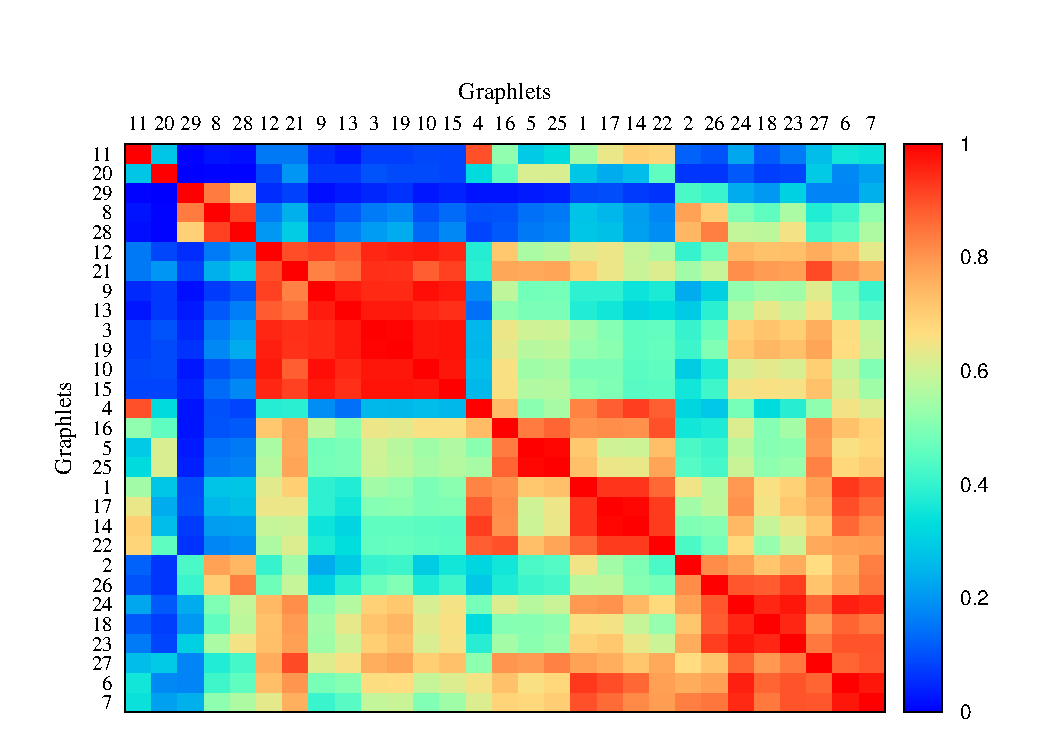
\includegraphics[scale=1.0]{../code/final_results/hsa_metabolic_network/heatmap_pearsons_hclust_hsa_metabolic_network-poly-32.pdf}}
  \caption[Pearson's GCV correlation matrix heat map for the compound-based Human Metabolic network.]{Pearson's GCV correlation matrix heat map for the compound-based Human Metabolic network. The heat map has been normalised with feature scaling and a $3^{rd}$ degree polynomial and hierarchically clustered.}
  \label{meta_heatmap_hclust_3}
\end{figure}

 
Furthermore, we notice that graphlets from clusters $A$,$B$ and $C$ also have a certain amount of inter-correlation between them, with inter-correlation values of at least 0.5. However, this is not the case for cluster $D$, which is made of cliques. The cliques only bear some correlation with cluster $C$ made of triangle-like graphlets, which is not surprising for the following reasons:
\begin{itemize}
 \item Cliques contain a lot of triangles
 \item Cliques do not contain claws $C_n$ or paths $P_n$, which miss several edges.
\end{itemize}

It should also be noted that graphlets $G_{11}$ and $G_{20}$ have been left outside, as they don't strongly correlate with any of the other groups. The cluster closest to these 2 graphlets is the claw cluster. To sum up, we conclude that graphlets cluster together according to what basic shapes they contain.

\subsection{Canonical Correlation Analysis}

In order to run Canonical Correlation Analysis on the metabolic networks we used \emph{Enzyme Commission} (EC) numbers as annotations for the network nodes. More information about EC numbers can be found in background section \ref{metabolic_annotations}. Basically, EC numbers are used to annotate each enzyme in the metabolic network according to the type of reaction it catalyses. The results of the CCA analysis using EC numbers is presented in figure \ref{hsa_metabolic_network_cca}.

\begin{figure}
  \begin{subfigure}{.65\textwidth}
  \centering
  \begin{tabular}{ c c | c c }
    \multicolumn{2}{c}{Canonical Correlation} &  \multicolumn{2}{c}{0.51769} \\
    \multicolumn{2}{c}{p-value} &  \multicolumn{2}{c}{0.00000} \\
    \hline
    \multicolumn{2}{c}{X variate} & \multicolumn{2}{c}{Y variate}\\
    \hline
  EC5 & -0.11422 &  G20 & -0.13839\\
  EC2 & -0.12601 &  G11 & -0.17646\\
  EC4 & -0.16144 &  G9 & -0.17733\\
  EC1 & -0.16156 &  G10 & -0.18420\\
  EC3 & -0.21057 &  G13 & -0.18757\\
  EC6 & -0.40615 &  G16 & -0.20243\\
  & &  G12 & -0.20399\\
  & &  G4 & -0.20521\\
  & &  G15 & -0.20553\\
  & &  G3 & -0.20671\\
  & &  G19 & -0.20956\\
  & &  G22 & -0.21329\\
  & &  G5 & -0.21897\\
  & &  G25 & -0.22033\\
  & &  G14 & -0.22256\\
  & &  G17 & -0.23125\\
  & &  G21 & -0.23144\\
  & &  G18 & -0.24860\\
  & &  G1 & -0.25408\\
  & &  G27 & -0.25641\\
  & &  G6 & -0.26110\\
  & &  G24 & -0.26365\\
  & &  G23 & -0.26813\\
  & &  G7 & -0.28239\\
  & &  G26 & -0.28362\\
  & &  G28 & -0.32754\\
  & &  G29 & -0.34583\\
  & &  G2 & -0.36785\\
  & &  G8 & -0.37442\\
  \end{tabular}

  \end{subfigure}
  \begin{subfigure}{.25\textwidth}
    \centering 
    \rowcolors{1}{}{}		
	
    \gtwenty
    \geleven
    \gnine
    \gdots
    \gtwentynine
    \gtwo
    \geight

  \end{subfigure}
  
\caption[CCA analysis on the compound-based Human Metabolic network.]{CCA analysis on the compound-based Human Metabolic network. The CCA is 0.51, with a p-value smaller than 0.0001. We notice that all EC numbers correlate positively with all the graphlets because their cross-loadings have the same sign. In the $X$ variate EC6 shows the highest correlation while in the $Y$ variate cliques \{8,2,29\} show the highest correlation. Note that the p-value is not exactly zero, but it was truncated to zero because of floating point approximations.}
\label{hsa_metabolic_network_cca}
\end{figure}

There is some degree of correlation between the Graphlets and the EC numbers ($\rho = 0.517 $), with a p-value smaller than 0.05. All the cross-loadings from both the graphlets and the EC numbers have the same sign, which suggests that they are positively correlated. Cliques \{8,2,29\} have the highest magnitude in their weights, while EC6 (ligands) have the highest magnitude in the EC vector. 

EC6 refers to Ligases, which are enzymes that can catalyse the joining of two large molecules by forming a new chemical bond. The reason why the magnitude of EC6 is quite high (0.4) compared to the other indicators is because the two large molecules catalysed by EC6 enzymes are represented in the metabolic network by cliques or dense clusters which have a lot of interactions and feedback loops between them. This is why cliques \{8,2,29\} or dense graphlets such as $G_{28}$ have the cross-loadings with the highest magnitude. However, this doesn't exclude other sparser protein groups to be part of the two molecules catalysed by the Ligase, since graphlets such as \{9,10,11 or 12\} also correlate positively with EC6. Regarding the other functional groups, we cannot say much about them because the magnitude of their cross-loading is relatively smaller compared to the cross-loading of EC6. 


\subsection{CCA Results for other model organisms}

We have analysed other compound-based metabolic networks that belong to the following organisms: C. elegans, D.melanogaster, E.coli, M.musculus, S.cerevisiae. These experiments confirm the results obtained for the human metabolic network. Average CCA correlation is around 0.5, EC6 has the highest magnitude at around 0.4 and cliques \{2,8,29\} are the graphlets most correlated with EC6 ($\rho = 0.35$).

The same methodology has also been applied to enzyme-based metabolic networks for all the 6 different organisms. However, these display a much lower CCA correlation (around 0.25), having p-values that are above 0.05, suggesting that the results are not statistically significant. This is the case for all the organisms, including humans. The graphlet signatures have very low signatures, while EC numbers don't have magnitudes above 0.22. These results have not been included in the report, but are available in the source code, under the \lstinline|code/final_results/| folder\footnote{The relevant folders are: \lstinline|hsa_meta_ec_omer|, \lstinline|cel_metabolic|, \lstinline|dme_metabolic|, \lstinline|eco_metabolic|, \lstinline|mmu_metabolic|, \lstinline|sce_metabolic|, }.

\subsection{CCA on the KEGG categories}

We have also tried to use the KEGG categories as annotations for the enzymes in the metabolic network. We have initially annotated the enzymes with the following high-level categories:
\begin{itemize}
 \item Metabolism
 \item Genetic Information Processing
 \item Environmental Information Processing
 \item Cellular Processes
 \item Organismal Systems
 \item Human Diseases
\end{itemize}

The CCA correlation obtained was only around 0.6, so we tried running CCA on the lower-level categories. That is, for each of those 6 high-level categories, we ran CCA on its subcategories. The best results were obtained for Human Diseases, Cellular Processes and Organismal Systems and are presented in the following subsections.

\subsection{Cellular Processes}
\label{cca_kegg_cellular}

The overall CCA correlation for Cellular Processes is 0.98, which is quite high compared to previous CCAs, and the p-value is smaller than 0.00001.  Figure \ref{cellular_cca} shows the CCA for Cellular Processes. We observe that graphlet $G_9$ correlates positively with \emph{Transport and Catabolism}. The reason for this is because in Catabolism, large molecules such as polysaccharides, lipids and nucleic acids are broken down into smaller units such as monosaccharides, fatty acids or nucleotides. Since molecules such as polysaccharides are made up of long chains of small monomer units, graphlets that are made of long paths such as $G_9$ will be overly represented in these processes. Similarly, enzymes involved in transport are transporting nutrients from one chemical to another, so their interactions will be characterised by long "transportation" paths that are best represented by graphlet $G_9$. 
At the other end of the spectrum, \emph{Cell growth and death} and \emph{Cell communication} are correlated with graphlets \{1,2,7,8\}. The reason for this is because in Cell Communication, if a cell is stimulated, it's needs to send signals to its neighbours through the use of molecules. First of all, in order to ensure that a signal is successfully transmitted, several molecules carrying the same message could be transmitted and there must be different possible paths to reach the destination. If this is not the case, then the message will get lost when the path is disrupted or the messenger molecule stops functioning. This is why a graphlet like $G_9$ correlates negatively with these, because $G_9$ is made of a long path of 5 nodes and if one of the nodes fails, then the whole signal is lost. Graphlets \{2,7,8\} correlate positively because these are highly connected (\{2,8\} are cliques) or because they contain several alternative paths for message transmission ($G_7$). However, the reason why graphlet $G_
1$ correlates with Cell Communication is still a matter or research.


\begin{figure}
  \begin{subfigure}{.65\textwidth}
  \centering
  \textbf{Cellular Processes CCA}\par\medskip
  \begin{tabular}{ c c | c c }
    \multicolumn{2}{c}{Canonical Correlation} &  \multicolumn{2}{c}{0.98633} \\
    \multicolumn{2}{c}{p-value} &  \multicolumn{2}{c}{0.00000} \\
    \hline
    \multicolumn{2}{c}{X variate} & \multicolumn{2}{c}{Y variate}\\
    \hline
  Transport and catabolism & 0.52121 &  G9 & 0.04828\\
  Cell motility & 0.20502 &  G21 & 0.01960\\
  Cell communication & -0.40751 &  G25 & 0.01441\\
  Cell growth and death & -0.69712 &  G5 & 0.01434\\
  & &  G16 & 0.00969\\
  & &  G13 & 0.00199\\
  & &  G12 & -0.00048\\
  & &  G27 & -0.00134\\
  & &  G20 & -0.00256\\
  & &  G3 & -0.00412\\
  & &  G24 & -0.01287\\
  & &  G19 & -0.01528\\
  & &  G10 & -0.01623\\
  & &  G18 & -0.01681\\
  & &  G14 & -0.02579\\
  & &  G11 & -0.02667\\
  & &  G23 & -0.02851\\
  & &  G15 & -0.03092\\
  & &  G17 & -0.03201\\
  & &  G29 & -0.04271\\
  & &  G6 & -0.04386\\
  & &  G28 & -0.04750\\
  & &  G4 & -0.05059\\
  & &  G26 & -0.05235\\
  & &  G22 & -0.05877\\
  & &  G8 & -0.05881\\
  & &  G7 & -0.07069\\
  & &  G2 & -0.07388\\
  & &  G1 & -0.07463\\
  \end{tabular}

  \end{subfigure}
  \begin{subfigure}{.25\textwidth}
    \centering 
    \rowcolors{1}{}{}		
	
    \gnine
    \gtwentyone
    \gtwentyfive
    \gdots
    \gseven
    \gtwo
    \gone

  \end{subfigure}
  
\caption[CCA on the Human Metabolic network using Cellular Processes from KEGG]{CCA on the Human Metabolic network using Cellular Processes from KEGG. The correlation value is high ($\rho = 0.98$) and the p-value is smaller than 0.00001, suggesting a very strong correlation. Transport and catabolism and cell motility correlate with the upper part of the graphlet spectrum: \{9,21,25,5, \dots\} because their cross-loadings have the same sign. Similarly, Cell Communication and Cell growth and death correlate with the lower end of the graphlet spectrum: \{1,2,7,8, \dots\}. }
\label{cellular_cca}
\end{figure}



\subsection{Organismal Systems}
\label{cca_kegg_organismal}

Figure \ref{organismal_cca} shows the CCA for \emph{Organismal Systems}. The CCA correlation is also very high (0.96) and the p-value smaller than 0.0001. These cross-loadings suggest that enzymes involved in Environmental Adaptation and Excretory systems are usually rich in interactions and their neighbours are also highly clustered, since all the graphlets correlate positively with these systems. On the other hand, enzymes involved in Circulatory and Digestive metabolic pathways have sparse  neighbourhoods that would ideally contain few graphlets. One explanation for this is because in these systems enzymes, proteins and metabolites have to circulate throughout the whole body and interact with distant enzymes, which don't cluster together. Enzymes at the other end of the spectrum (Environmental Adaptation and Excretory system) are much more localised in the body. For instance, excretory system enzymes are mainly active in the kidney or liver. Moreover, the enzymes involved in the Circulatory and Digestive 
systems will probably have less interactions compared to their counterparts in the Environmental Adaptation and Excretory systems, because a neighbourhood sparse in graphlets is usually an indication of it being small.



\begin{figure}
  \centering
  \textbf{Organismal Systems CCA}\par\medskip
  \begin{subfigure}{.65\textwidth}
  \centering
  \begin{tabular}{ c c | c c }
    \multicolumn{2}{c}{Canonical Correlation} &  \multicolumn{2}{c}{0.96925} \\
    \multicolumn{2}{c}{p-value} &  \multicolumn{2}{c}{0.00000} \\
    \hline
    \multicolumn{2}{c}{X variate} & \multicolumn{2}{c}{Y variate}\\
    \hline
  Environmental adaptation & 0.20426 &  G26 & 0.30978\\
  Excretory system & 0.19729 &  G24 & 0.29818\\
  Development & 0.07461 &  G23 & 0.29308\\
  Endocrine system & 0.04192 &  G18 & 0.28901\\
  Nervous system & -0.01315 &  G6 & 0.27857\\
  Sensory system & -0.06276 &  G12 & 0.26520\\
  Immune system & -0.15192 &  G19 & 0.25419\\
  Digestive system & -0.23211 &  G3 & 0.24988\\
  Circulatory system & -0.37659 &  G14 & 0.23274\\
  & &  G13 & 0.23155\\
  & &  G1 & 0.22611\\
  & &  G17 & 0.22546\\
  & &  G7 & 0.21225\\
  & &  G27 & 0.20440\\
  & &  G10 & 0.19976\\
  & &  G9 & 0.19547\\
  & &  G25 & 0.19422\\
  & &  G16 & 0.19135\\
  & &  G28 & 0.18874\\
  & &  G4 & 0.18421\\
  & &  G5 & 0.18381\\
  & &  G20 & 0.17359\\
  & &  G11 & 0.15537\\
  & &  G21 & 0.14453\\
  & &  G29 & 0.11208\\
  & &  G8 & 0.10681\\
  & &  G2 & 0.10369\\
  & &  G22 & 0.08192\\
  & &  G15 & 0.01276\\
  \end{tabular}

  \end{subfigure}
  \begin{subfigure}{.25\textwidth}
    \centering 
    \rowcolors{1}{}{}		
	
    \gtwentysix
    \gtwentyfour
    \gtwentythree
    \gdots
    \gtwo
    \gtwentytwo
    \gfifteen

  \end{subfigure}
  
\caption[CCA on the Human Metabolic network between different Organismal Systems and the GCV signature of enzymes.]{CCA on the Human Metabolic network between different Organismal Systems and the GCV signature of enzymes. The correlation value is again high ($\rho = 0.96$) and the p-value is small ($p < 0.00001$). Environmental adaptation, Excretory system, Development and the Endocrine system correlate positively with all the graphlets, while the Circulatory, Digestive, Immune, Sensory and Nervous systems correlate negatively. The actual p-value is not exactly zero but it is shown as zero because of floating point approximations.}
\label{organismal_cca}
\end{figure}




\subsection{Human Diseases}
\label{cca_kegg_human}

Figure \ref{fig:metabolic_diseases_cca} shows the CCA for various Human Diseases such as Cancers, Immune diseases, Neurodegenerative diseases or Cardiovascular diseases. The result that is most striking here is that Cardiovascular diseases and Substance dependence correlate negatively with almost all the graphlets (apart from \{2,8\}). This implies that the enzymes and proteins involved in these Human Diseases have a low number of interactions and when they do have interactions, their neighbourhood only contains small clusters of 3--4 nodes maximum. The explanation for this might be the same as for the Organismal Systems: the enzymes involved in Cardiovascular diseases and Substance dependence travel across long pathways throughout the body and end up interacting with distant chemicals that do not interact with each other because of their distant location in the body. However, the small clusters of interactions might occur because of locality, that is all chemicals involved will be in the same area and 
therefore inevitably interact with each other. In the case of the Cardiovascular diseases, the enzymes travel long distances because they are transported through the blood vessels, while the ones involved in Substance dependence are again transported through the blood vessels or other channels. We cannot say anything about the rest of the diseases (Cancers, Immune Diseases, etc \dots) because their relative cross-loadings have a very low magnitude relative to the others.


\begin{figure}
  \centering
  \textbf{Human Diseases CCA}\par\medskip
  \begin{subfigure}{.65\textwidth}
  \centering
  \begin{tabular}{ c c | c c }
    \multicolumn{2}{c}{Canonical Correlation} &  \multicolumn{2}{c}{0.99479} \\
    \multicolumn{2}{c}{p-value} &  \multicolumn{2}{c}{0.00000} \\
    \hline
    \multicolumn{2}{c}{X variate} & \multicolumn{2}{c}{Y variate}\\
    \hline
  Cardiovascular diseases & 0.99171 &  G2 & 0.01681\\
  Substance dependence & 0.57989 &  G8 & 0.00462\\
  Infectious diseases & 0.21844 &  G29 & -0.00737\\
  Neurodegenerative diseases & 0.00366 &  G7 & -0.00812\\
  Endocrine and metabolic diseases & -0.02545 &  G1 & -0.00989\\
  Immune diseases & -0.03029 &  G26 & -0.01077\\
  Cancers & -0.08682 &  G24 & -0.01274\\
  & &  G6 & -0.01321\\
  & &  G28 & -0.01321\\
  & &  G15 & -0.01342\\
  & &  G23 & -0.01369\\
  & &  G22 & -0.01420\\
  & &  G21 & -0.01438\\
  & &  G14 & -0.01449\\
  & &  G12 & -0.01465\\
  & &  G17 & -0.01516\\
  & &  G16 & -0.01521\\
  & &  G18 & -0.01526\\
  & &  G13 & -0.01528\\
  & &  G19 & -0.01562\\
  & &  G9 & -0.01565\\
  & &  G10 & -0.01641\\
  & &  G4 & -0.01727\\
  & &  G3 & -0.01742\\
  & &  G11 & -0.01781\\
  & &  G20 & -0.01936\\
  & &  G25 & -0.02017\\
  & &  G5 & -0.02438\\
  & &  G27 & -0.02731\\
  \end{tabular}


  \end{subfigure}
  \begin{subfigure}{.25\textwidth}
    \centering 
    \rowcolors{1}{}{}		
	
    \gtwo
    \geight
    \gtwentynine
    \gdots
    \gtwentyfive
    \gfive
    \gtwentyseven

  \end{subfigure}
  
\caption[CCA Analysis on the Human Metabolic network between Human Diseases and the GCV signature.]{CCA Analysis on the Human Metabolic network between Human Diseases and the GCV signature. The correlation value is high ($\rho = 0.96$) while the p-value is very small ($p < 0.00001$). The actual p-value outputted by the program is 0.0 due to floating-point approximations. Cardiovascular diseases, Substance dependence, Infectious and Neurodegenerative diseases correlate positively with all the graphlets, while the Endocrine and Metabolic diseases, Immune diseases and Cancers correlate negatively.}
\label{fig:metabolic_diseases_cca}
\end{figure}







% Chapter 5
\chapter{Evaluation}
\label{chp:evaluation}
% Be warned that many projects fall down through poor evaluation. Simply building a system and documenting its design and functionality is not enough to gain top marks. It is extremely important that you evaluate what you have done both in absolute terms and in comparison with existing techniques, software, hardware etc. This might involve quantitative evaluation, for example based on numerical results, performance etc. or something more qualitative such as expressibility, functionality, ease-of-use etc. At some point you should also evaluate the strengths and weaknesses of what you have done. Avoid statements like "The project has been a complete success and we have solved all the problems asssociated with blah...; - you will be shot down immediately! It is important to understand that there is no such thing as a perfect project. Even the very best pieces of work have their limitations and you are expected to provide a proper critical appraisal of what you have done.

\section{Strengths and weaknesses}

The GCV signature has been successfully used on some of the networks and it helped us get valuable insights. The best results have been obtained on the WTN networks, followed by the PPI and metabolic networks. Overall, the main achievements of this project are as follows:
\begin{itemize}
 \item The development of the mathematical model of the GCV signature followed by the implementation and parallelisation of the algorithm that computes it.
 \item The use of a rigorous methodology for the analysis of GCV correlations that helped us uncover insights from the network data.
 \item The results and interpretations presented for the economic, protein interaction and metabolic networks.
 \item The quantitative evaluation of the GCV signature (sections \ref{sec:eval_clust} and \ref{sec:eval_classify}).
\end{itemize}

However, the GCV signature has inherent limitations and weaknesses. The main deficiencies with our methodology are:
\begin{itemize}
 \item A more effective normalisation method of the GCV can be designed. Such a normalisation method can take into account the size of the neighbourhood subgraph.
 \item A redundancy analysis of each GCV frequency has not been made. This could tell us whether elements in the GCV vector are redundant and eliminating these will improve the GCV performance and remove noise.
 \item The GCV signature is only able to quantify the structure between the immediate neighbours of a node. It cannot capture the structure between nodes that are further away from the source node, at distances of 2 or more. 
 \item The implementation of the GCV computation is not parallelisable on a cluster of computers. The program is only able to spawn processes that run on multiple cores. Moreover, when using multiple processes for parallel GCV computation, most of the processes finish their share early while a few processes get stuck with computing GCVs for hub nodes. This problem could be overcome by redistributing the workload to the processes that finish early.
 \item The GCV signature is not able to capture any information in some of the networks, such as the enzyme-based metabolic network. Further research needs to be done in order to understand why that is the case.
 \item The results we got for the WTN, PPI and Metabolic networks need more supporting experiments in order to validate the interpretations. 
\end{itemize}


\section{Evaluation of network clustering}
\label{sec:eval_clust}

Although the focus of this project is on using the GCV signature for uncovering hidden structures in the data analysed, we are also interested to find out whether the GCV can be used for clustering networks of different types. In this section, we evaluate the performance of the GCV signature on clustering the following types of random graphs:
\begin{itemize}
 \item Erd\H{o}s-R\'{e}nyi graphs (ER)
 \item Erd\H{o}s-R\'{e}nyi graphs with preserved degree distribution (ER-DD)
 \item Geometric graphs (GEO)
 \item Scale-free Barab\'{a}si-Albert graphs (preferential attachment) (SF-BA)
 \item Stickiness index-based graphs (STICKY)
\end{itemize}

For each model, we generate 30 different networks that are modelled from the 2010 World Trade network. These random networks have also been used in section \ref{sec:initial_experiments_rnd_nets} for computing the average network GCVs. For each one of the 150 generated networks, we compute 6 different signatures:
\begin{enumerate}
 \item Graphlet Cluster Vector (GCV)
 \item Degree Distribution
 \item Average clustering coefficient
 \item Spectral distribution
 \item Graphlet Frequency Vector (GFV).
 \item Graphlet Distribution Vector (GDV).  
\end{enumerate}

Calculating each of the 6 signatures requires a considerable amount of computation. This is the reason why we have chosen to generate the random networks from the WTNs, because these networks are small in comparison to the metabolic or PPI networks. Other networks such as the PPI networks are much larger and computation of all the signatures on 150 of these networks is very intense. 

After all signatures for the 150 networks have been calculated, the distance between each pair of networks is computed. All these entries are placed in a 150x150 distance matrix and 6 distance matrices are finally obtained, one for each signature. The distance matrices can be used for visualising the distances using \emph{Multi-dimensional scaling} or for performing Precision-Recall curve analysis or Receiver-Operating Characteristic (ROC) curve analysis. These results are presented in the next sections. 

The Relative Graphlet Frequency distance (RGFD) defined in section \ref{sec:rgfd} has been used as the distance metric between two Graphlet Frequency Vectors. For the distance metric between two Graphlet Distribution Vectors, we have used the Graphlet Correlation Distance defined in section \ref{pearsons_background}. This will be denoted as GCD73, because it uses information from all 73 orbits and in order to distinguish it from a similar metric called GCD-11 that has been developed by Yavero\u{g}lu et al \cite{yaverouglu2014revealing}. For the degree and spectral distributions, we have used as the Euclidean distance between the first 60 elements.\footnote{These distributions are in theory infinite so we decided to cap them at 60, since very little information is retained after this threshold.}

\section{Multi-dimensional scaling results}

Multi-dimensional scaling (MDS) refers to a series of visualisation techniques which attempts to represent $n$-dimensional data points into a 2D or 3D space such that the distances between them are preserved as much as possible. We computed 3D MDS plots for each of the 6 signatures using the \lstinline|Python Scikit| library which provides the function \lstinline|sklearn.manifold.MDS| that can perform the MDS transformation. 

Figures \ref{fig:gcv_mds} and \ref{fig:clust_coeff_mds} provide the 3D MDS plots for the GCV and the Clustering coefficient. For the GCV MDS plot, the ER networks are more spread compared to the other random graphs and clearly distanced from them. On the other hand, the distances between the ER-DD, STICKY and SF-BA graphs are really small, suggesting that the GCV signature cannot easily distinguish between these random networks. We also notice that the SF-BA random graphs have formed two different clusters. This phenomena might be explained by the fact that the SF-BA random graphs are very sensitive to the initial starting graph.  We therefore conclude that the GCV signature can only distinguish the ER networks from the rest. 

For the Clustering coefficient MDS, the data points are positioned in a nearly collinear fashion, because the clustering coefficient is a 1-dimensional signature. The ER-DD and Stickiness graphs show some degree of overlap\footnote{this fact is not completely obvious from the graph because the STICKY data points are covering the corresponding ER-DD data points.}, while the rest of the random graphs are clearly separated from each other. This means that the clustering coefficient is able to distinguish any two pairs of random graphs apart from a STICKY, ER-DD network pair.


\begin{figure}[H] 
  \captionsetup{width=8cm}
  \hspace{-2.0em}
  \begin{minipage}[b]{0.55\linewidth}
    \centering
    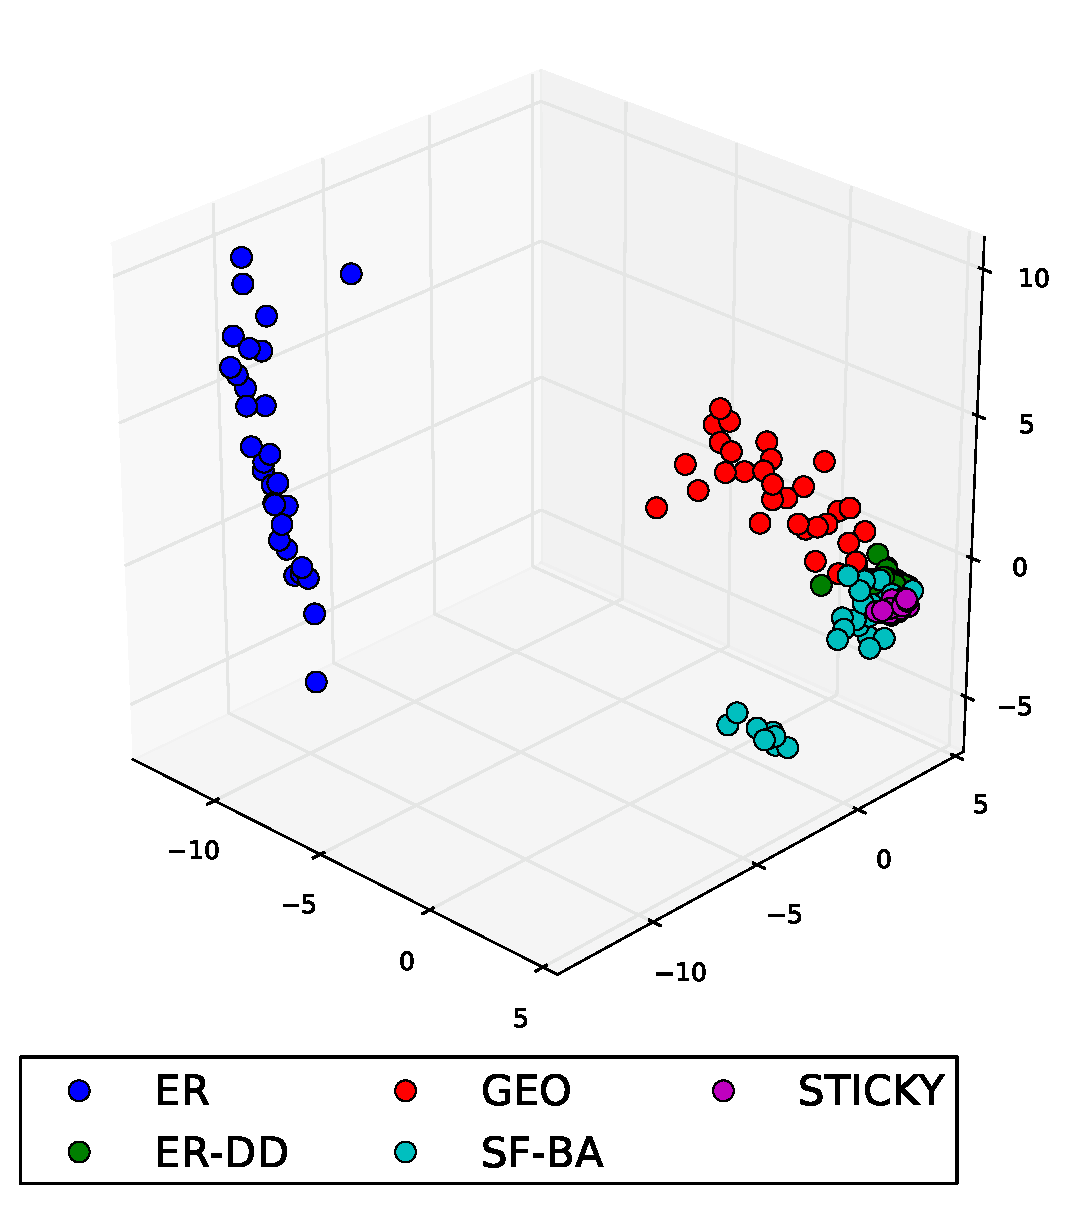
\includegraphics[scale=0.45]
    {../code/final_results/trade_2010_thresholded/eval_results/gcv_mds.pdf}
    \caption[Graphlet Cluster Vector MDS]{GCV MDS: The GCV signature cannot distinguish between ER-DD, GEO, SF and STICKY random graphs. The intra-cluster variance for ER networks is high.}
    \label{fig:gcv_mds}
%     \vspace{0.0ex}
  \end{minipage}%%
%   \hspace{0.5cm}
  \begin{minipage}[b]{0.55\linewidth}
    \centering
    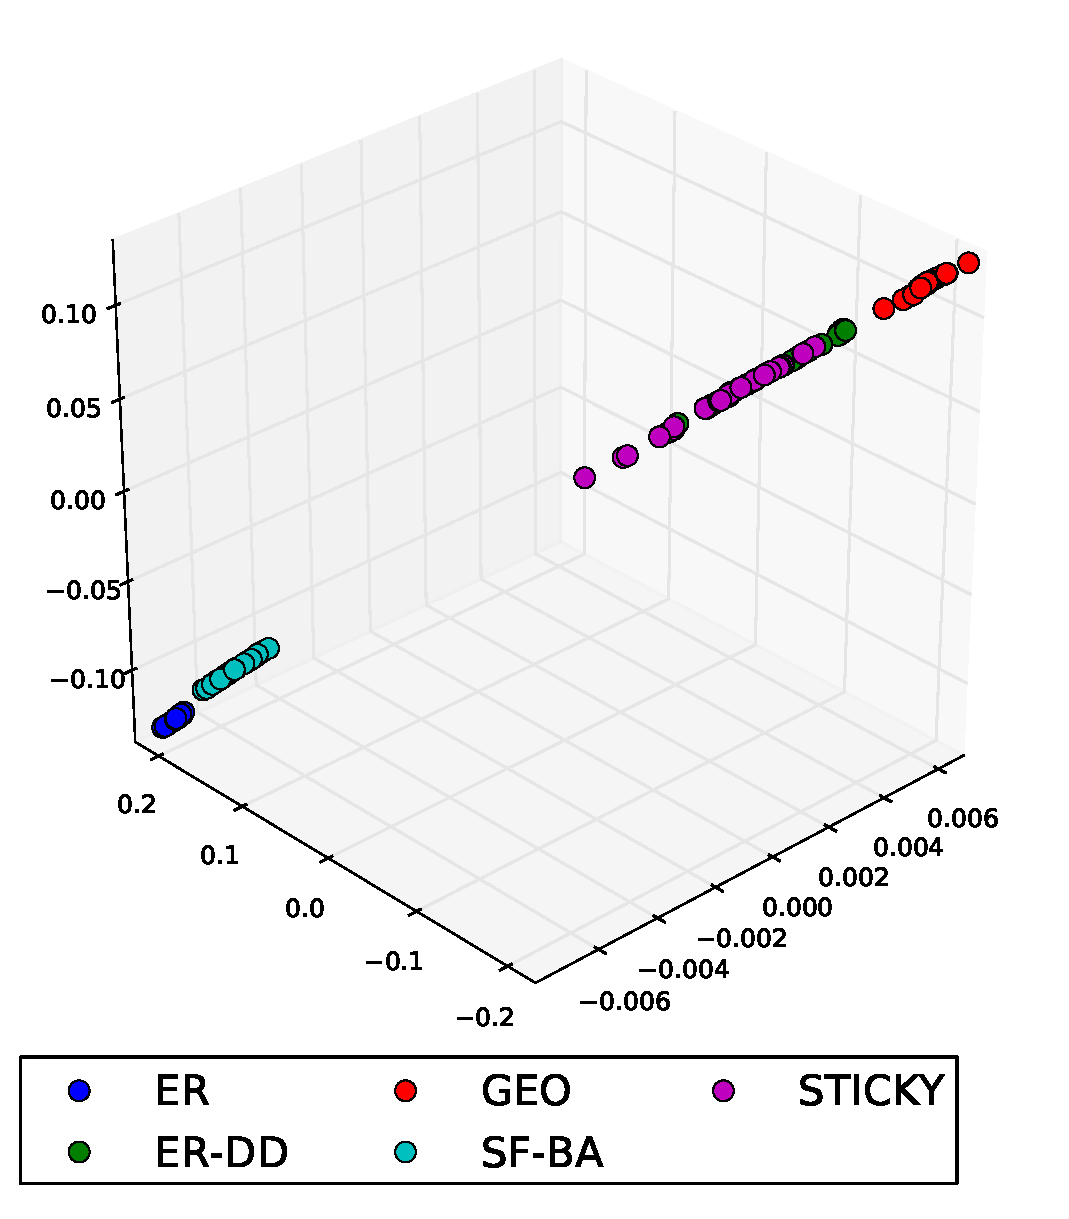
\includegraphics[scale=0.45]
    {../code/final_results/trade_2010_thresholded/eval_results/clust_coeff_mds.pdf}
    \caption[Clustering Coefficient MDS]{Clustering Coefficient MDS: The clustering coefficient cannot distinguish between ER-DD and STICKY random graphs (ER-DD points are hidden behind the STICKY points).}
    \label{fig:clust_coeff_mds}
%      \vspace{-1.0ex}
  \end{minipage} 
\label{fig:gcv_clust_mds} 
\end{figure}

The RGFD and GCD73 MDS plots are shown in figures \ref{fig:gfv_mds} and \ref{fig:gcd73_mds} respectively. The RGFD MDS shows that each of the clusters is clearly separated from the other, suggesting that RGFD is highly suitable for separating these types of networks. The GCD-73 metric is also suitable for clustering random networks, but the clusters display a higher variance.

\begin{figure}[H]
  \captionsetup{width=8cm}
  \hspace{-2.0em}
  \begin{minipage}[b]{0.55\linewidth}
    \centering
    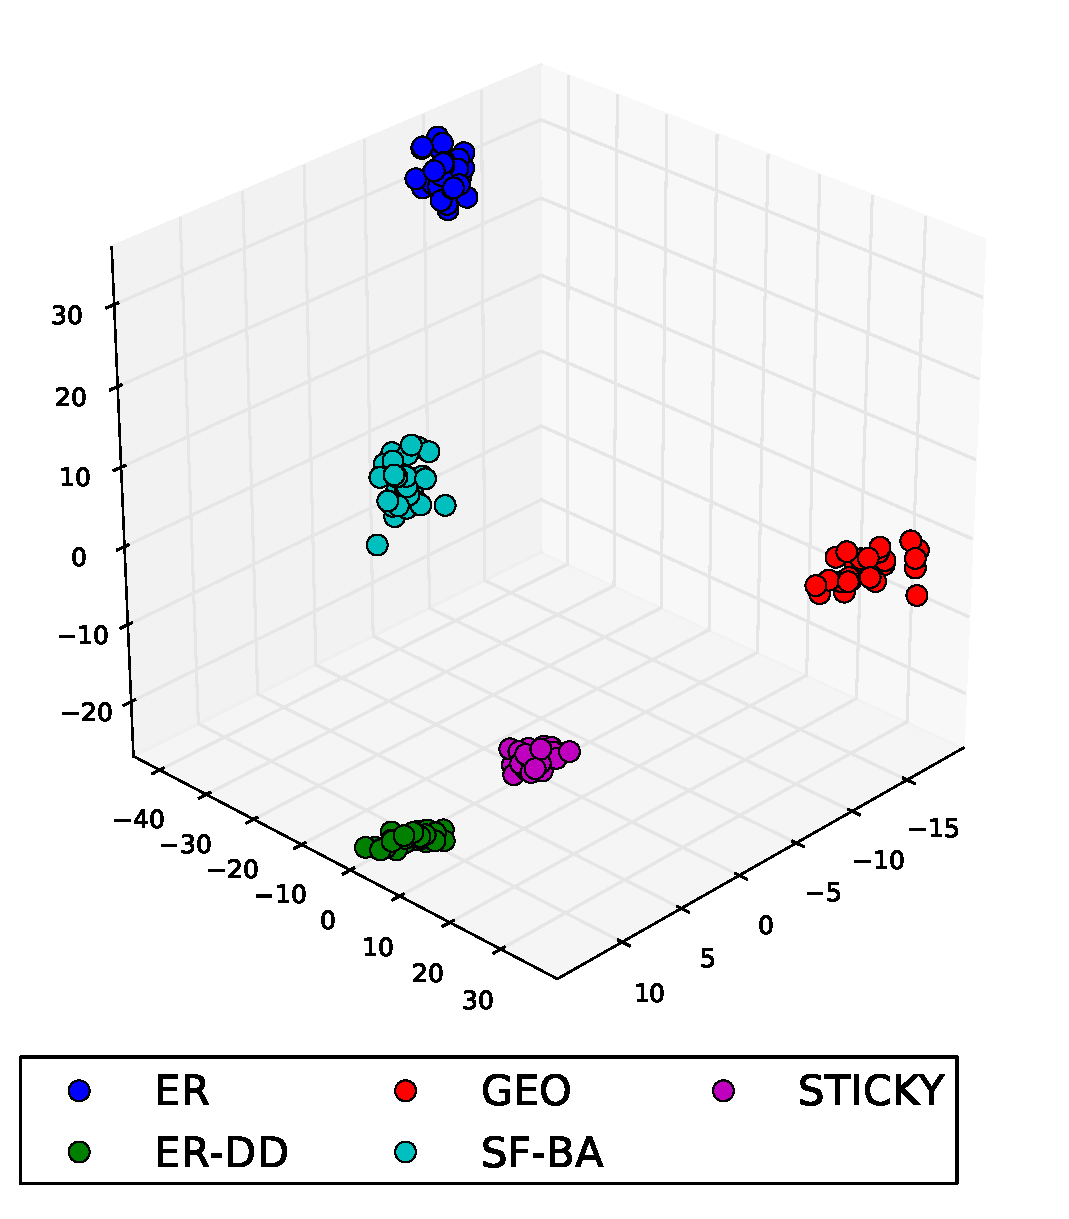
\includegraphics[scale=0.45]
    {../code/final_results/trade_2010_thresholded/eval_results/rgfd_mds.pdf}
    \caption[Relative Graphlet Frequency distance MDS]{RGFD MDS: The RGFD is clearly able to separate all the random network models. The intra-cluster variance is low.}
    \label{fig:gfv_mds}
  \end{minipage}%% 
%   \hspace{1.0em}
  \begin{minipage}[b]{0.55\linewidth}
    \centering
    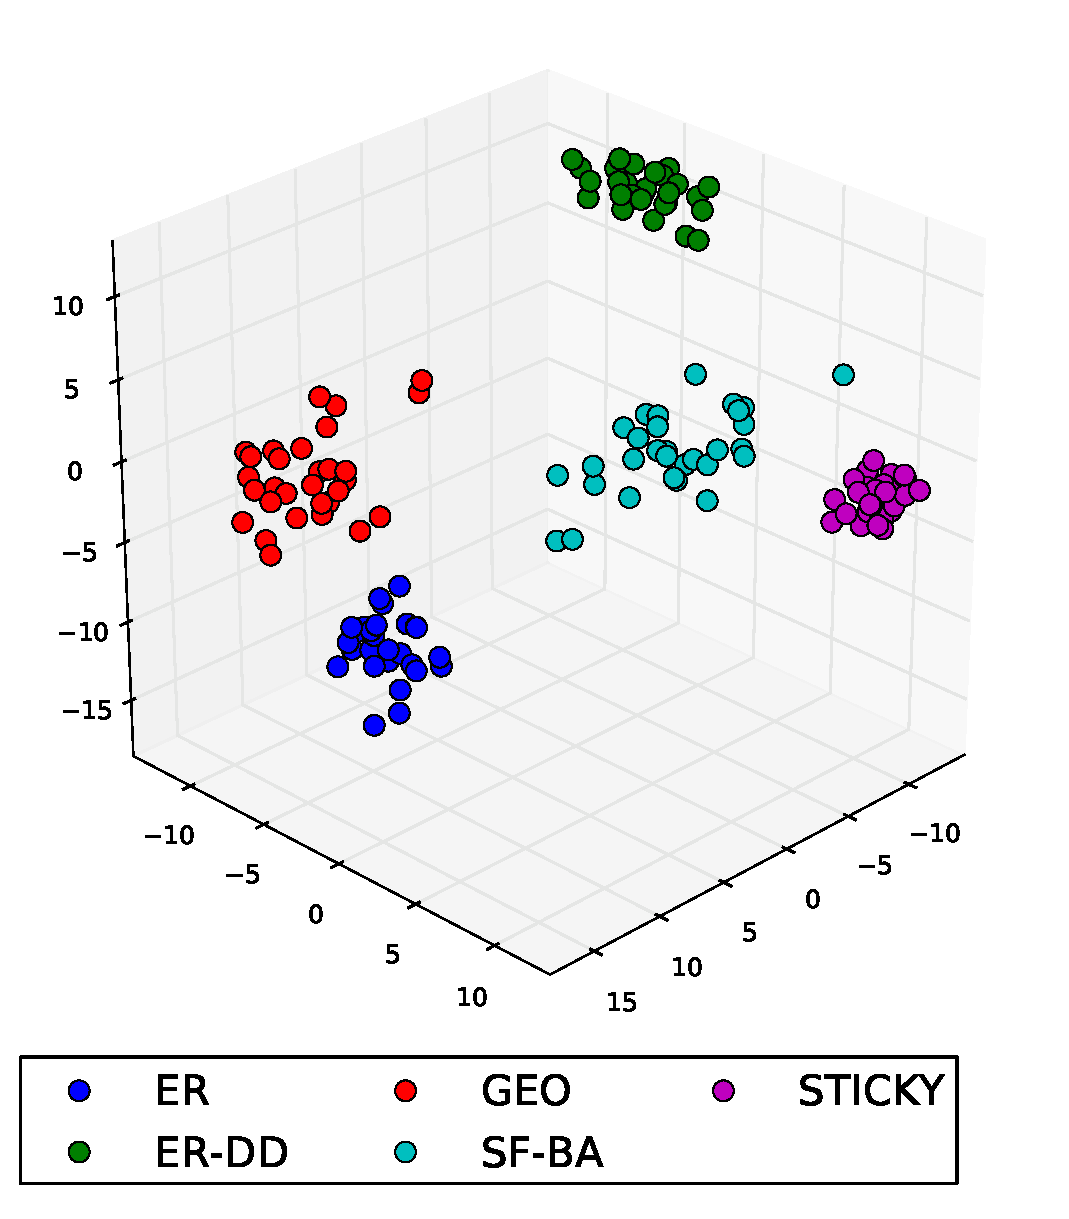
\includegraphics[scale=0.45]
    {../code/final_results/trade_2010_thresholded/eval_results/gcd73_mds.pdf}
    \caption[Graphlet correlation distance (GCD73) MDS]{GCD73 MDS: The GCD73 metric is also efficient at clustering random networks although the clusters are more spread around.}
    \label{fig:gcd73_mds}
%     \vspace{-1.0ex}
  \end{minipage} 
  \label{fig:rgfd_gdv_mds}
\end{figure}

Figures \ref{fig:degree_distrib_mds} and \ref{fig:spectral_distrib_mds} provide the 3D MDS plots for the Degree distribution and the Spectral Distribution signatures. The GEO and ER clusters in the Degree distribution MDS show a certain degree of overlap, although in reality there is much less overlap because the viewing angle is unsuitable\footnote{We tried to capture the image from other angles but that resulted in other clusters colliding.}. In the Spectral Distribution MDS, we notice that the ER and GEO clusters are very close to each other, suggesting that the Spectral Distribution cannot easily distinguish between these two types of random networks. However, the other clusters are clearly separated from each other.  

\begin{figure}[H]
  \captionsetup{width=8cm}
  \hspace{-2.0em}
  \begin{minipage}[b]{0.55\linewidth}
    \centering
    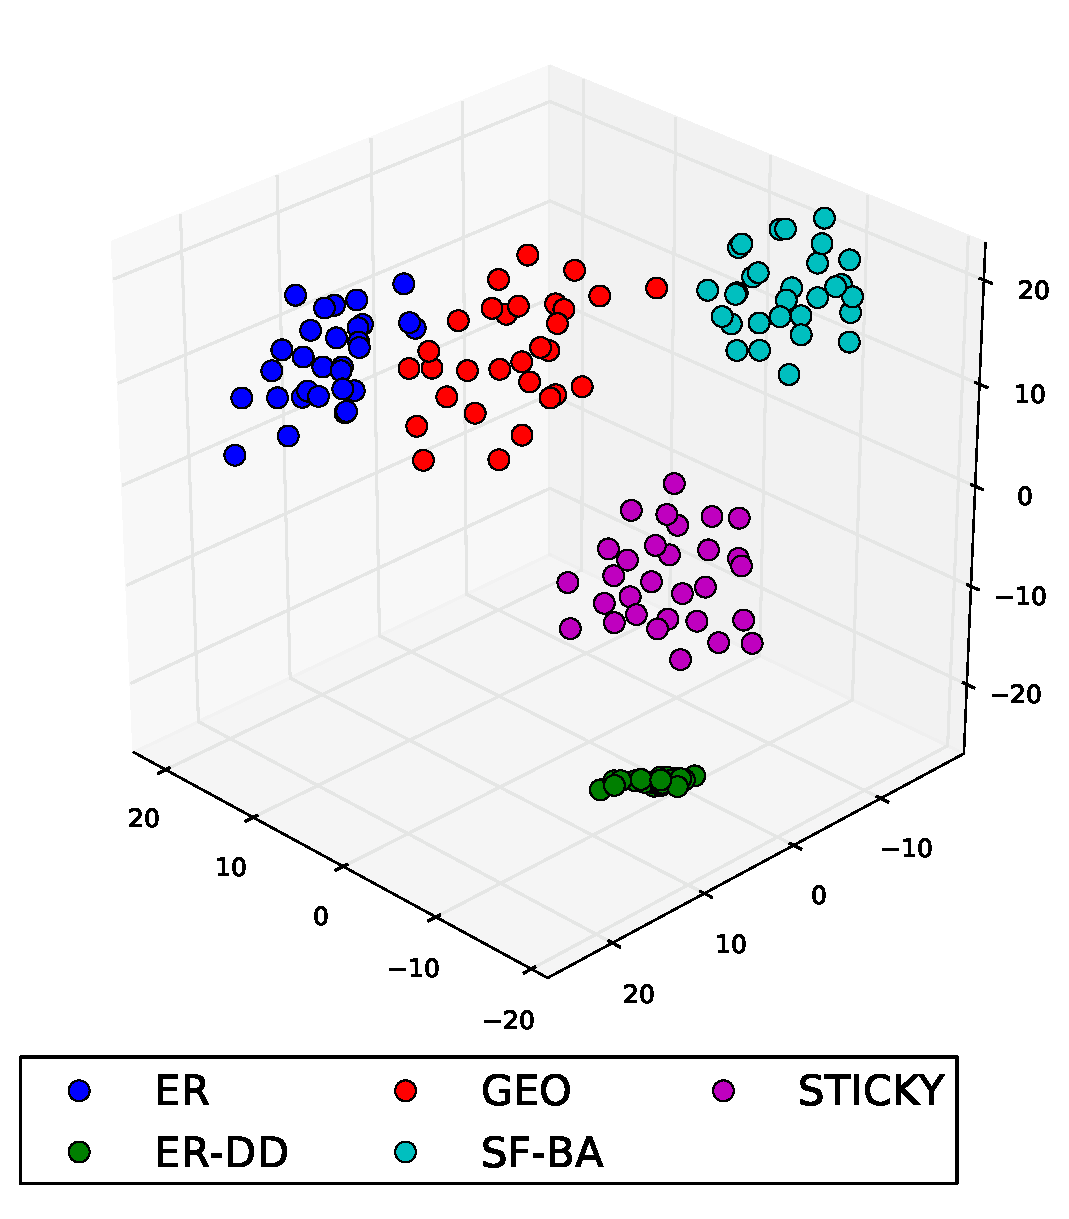
\includegraphics[scale=0.45]
    {../code/final_results/trade_2010_thresholded/eval_results/deg_distrib_mds.pdf}
    \caption[Degree Distribution MDS]{Degree Distribution MDS: Most of the clusters are clearly separated although the intra-cluster variance for ER, GEO, SF-BA and STICKY is high.}
    \label{fig:degree_distrib_mds}
  \end{minipage}%% 
  \begin{minipage}[b]{0.55\linewidth}
    \centering
    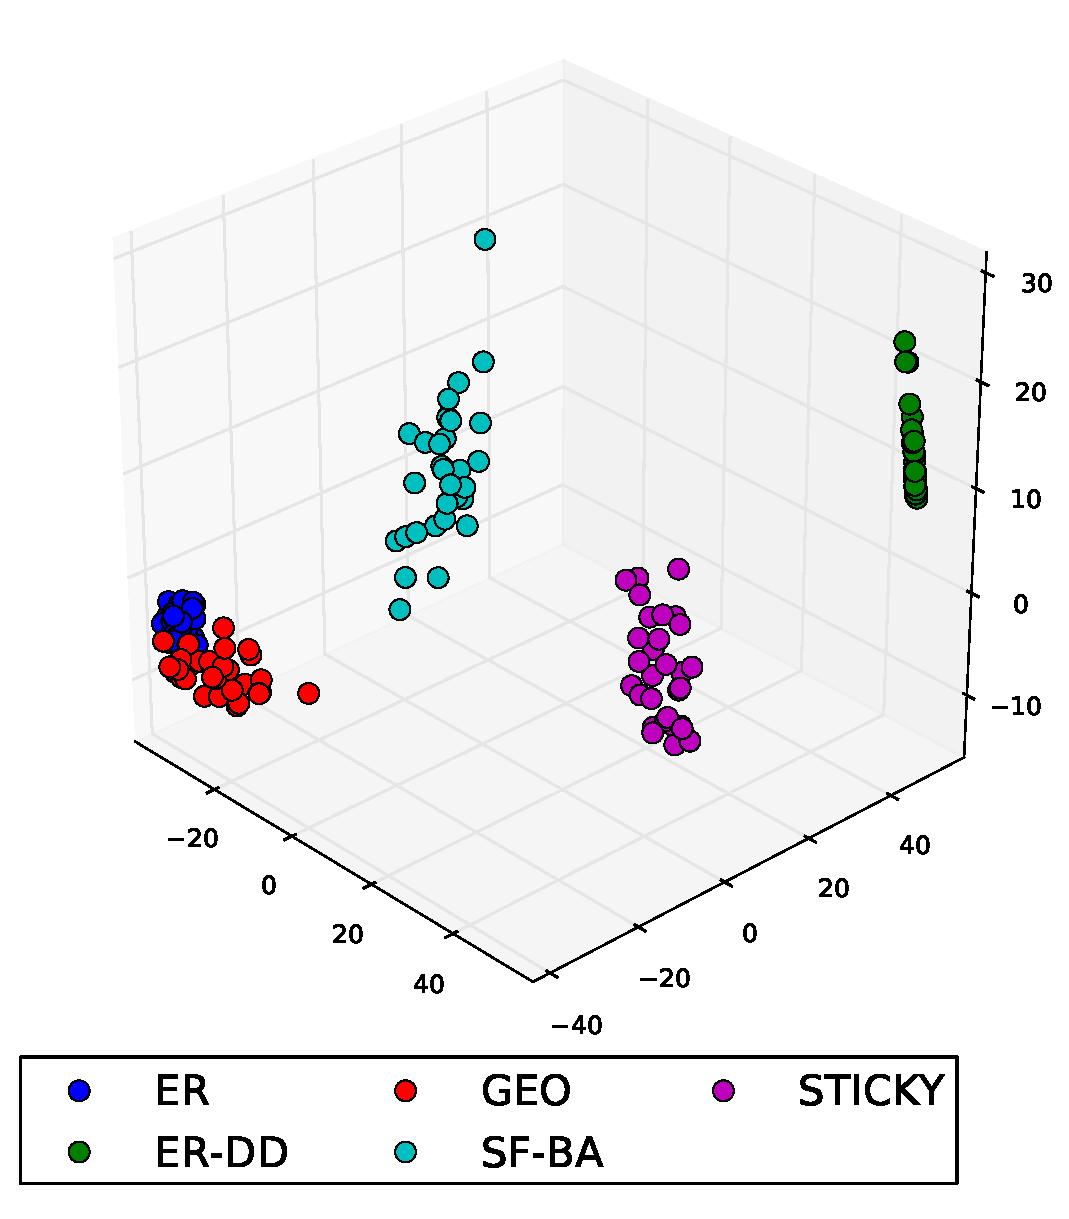
\includegraphics[scale=0.45]
    {../code/final_results/trade_2010_thresholded/eval_results/spectral_distrib_mds.pdf}
    \caption[Spectral Distribution MDS]{Spectral Distribution MDS: The spectral distribution cannot distinguish between ER and GEO random graphs. The other pairs of clusters are clearly separated.}
    \label{fig:spectral_distrib_mds}
%     \vspace{-1.0ex}
  \end{minipage} 
\end{figure}

\section{Precision-Recall curve}

MDS plots are only useful for visualising the distance matrices. However, one can test how well a distance measure groups networks of the same type by using the Precision-Recall curve. Starting from the 150x150 distance matrix, a Precision-Recall curve analysis can be performed in the following manner:
\begin{enumerate}
 \item one searches for the minimum and maximum distance in the distance matrix.
 \item for small increments of parameter $\epsilon$ such that $ min \le \epsilon \le max$, if the distance between two networks is smaller than $\epsilon$ then the pair of networks is retrieved
  \begin{enumerate}
  \item Precision is calculated as the fraction of the correctly retrieved pairs (i.e.\ grouping networks from the same model)
  \item Recall is calculated as the fraction of the correctly retrieved pairs over all the correct ones. 
  \end{enumerate}
 \item The Precision-Recall curve is plotted using the values calculated so far. 
 \item The Area under Precision-Recall (AUPR) can be calculated using the following formula:
	$$ AUPR = AUPR + 0.5 * (REC[k]-REC[k-1])*(PREC[k]+PREC[k-1]) $$
\end{enumerate}

We chose to perform a Precision-Recall curve analysis because it is known to be more robust to large numbers of negatives than Receiver Operator Characteristic (ROC) curve analysis \cite{davis2006relationship}. In our case negatives are pairs of networks that are grouped together although they belong to different random models.

Figure \ref{fig:prec_rec} shows the precision-recall curve for the six signatures calculated from their distance matrices. Our novel GCV signature has a generally low precision compared to the other signatures, as the precision decreases a lot in the recall range [0.2 -- 0.5]. This result was expected from our signature, since the MDS plots showed that it cannot easily distinguish between ER-DD, STICKY, SF-BA and GEO random graphs (figure \ref{fig:gcv_mds}). The best-performing signature is actually the RGFD, which has a precision of 1 for any recall value in range [0 -- 1]. Note that this is only faintly seen on the plot, because the GCD73 line overwrites it.
\begin{figure}[H]
  \hspace{-1.5em}
%   \centering
  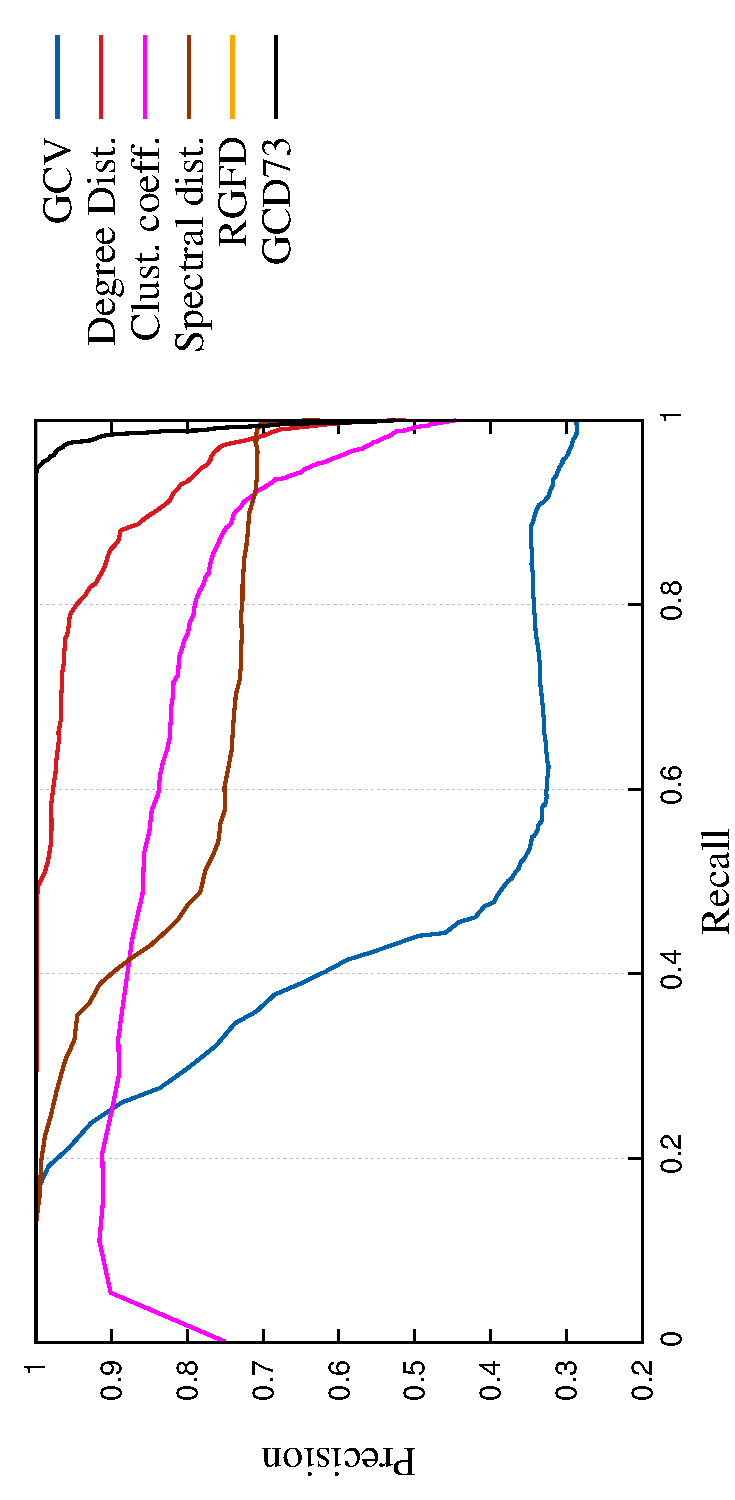
\includegraphics[scale=0.7, angle=-90]
  {../code/final_results/trade_2010_thresholded/eval_results/prec_rec_all_rnd_rew_02.pdf}
  \caption[Precision-Recall curves for GCV and 5 other signatures]{Precision-Recall curves for 6 different signatures: Graphlet Cluster Vector (GCV), Degree Distribution, Clustering Coefficient, Spectral Distribution, the Relative Graphlet Frequency distance (RGFD) and the Graphlet Correlation distance which uses the 73 automorphism orbits (GCD73). The best performing signature is the RGFD which has a value of 1 for any recall value. However, this is not clearly seen in the plot because the GCD73 line overwrites it. The GCV signature has the worst performance particularly in the range [0.25--1].}
  \label{fig:prec_rec}
\end{figure}

Table \ref{tab:aupr} shows the table of AUPR values for each of the signatures. The higher the AUPR, the better the signature is at distinguishing between different clusters. The best-performing distance measure is the RGFD that uses the \emph{Graphlet Frequency Vector} of the random network. It has a perfect AUPR of 1.0, which is expected because the RGFD MDS plot showed it can clearly distinguish all the random graphs generated. On the opposite end, our GCV signature has the worst AUPR of only 0.575. This suggests that the GCV signature is not suitable for clustering random networks generated from the WTN. 

\begin{table}[H]
  \centering
  \begin{tabular}{  c | c }
    GCV & 0.575\\
    \hline
    Degree Distribution & 0.949\\
    Clustering Coefficient & 0.829\\
    Spectral Distribution & 0.840\\
    RGFD & \textbf{1.0}\\
    GCD73 & 0.994\\
  \end{tabular}
  \caption{AUPR table for the GCV and other signatures. The best AUPR has been obtained using the GCD73 signature, which has an AUPR of 0.994. On the other hand, our GCV signature performed worst with an AUPR of 0.575.}
  \label{tab:aupr}
\end{table}


\section{Robustness testing}

This section evaluates the robustness of the six signatures. The same Precision-Recall curve analysis is performed, this time with data that is noisy, incomplete or when the signatures are approximated. However, because of the sheer number of experiments performed, only the final AUPR values are plotted. The methodology is similar to that performed by Yavero\u{g}lu et al. on the short GCD-11 signature \cite{yaverouglu2014revealing}. 

\subsection{Network Rewiring}

In most real-life scenarios the data we have to work with is noisy. In order to evaluate the GCV robustness to noise, we take each of our initial 150 generated random networks and rewire the edges with a probability $p$, for different values of $p$ between 0 and 1. When rewiring an edge $(i,j)$, we find a target node $k$ such that there is no edge between nodes $i$ and $k$. For each rewiring probability $p$ we get 150 different networks that have been rewired. Afterwards, we calculate the AUPR for this set of networks. Figure \ref{fig:rew_aupr} shows the AUPR for each signature as $p$ increases from 0\% to 90\%. All signatures apart from GCV and clustering coefficient show a general downward trend. The GCV reaches a low point in AUPR for a rewiring rate of $50\%$, but it increases again shortly afterwards. On the other hand, the clustering coefficient reaches a maximal AUPR when $p = 0.3$, followed by a sharp drop afterwards. When the networks are almost random ($p = 0.9$), the values of the AUPR converge to 
the range [0.5,0.7] for all signatures. 

We therefore conclude that the GCV signature is not robust to noisy data either, with other signatures such as RGFD always having an AUPR that is higher, for all rewiring rates. The best performing signature is again the RGFD which always has an AUPR above 0.6.
\begin{figure}[H]
  \hspace{-1.5em}
  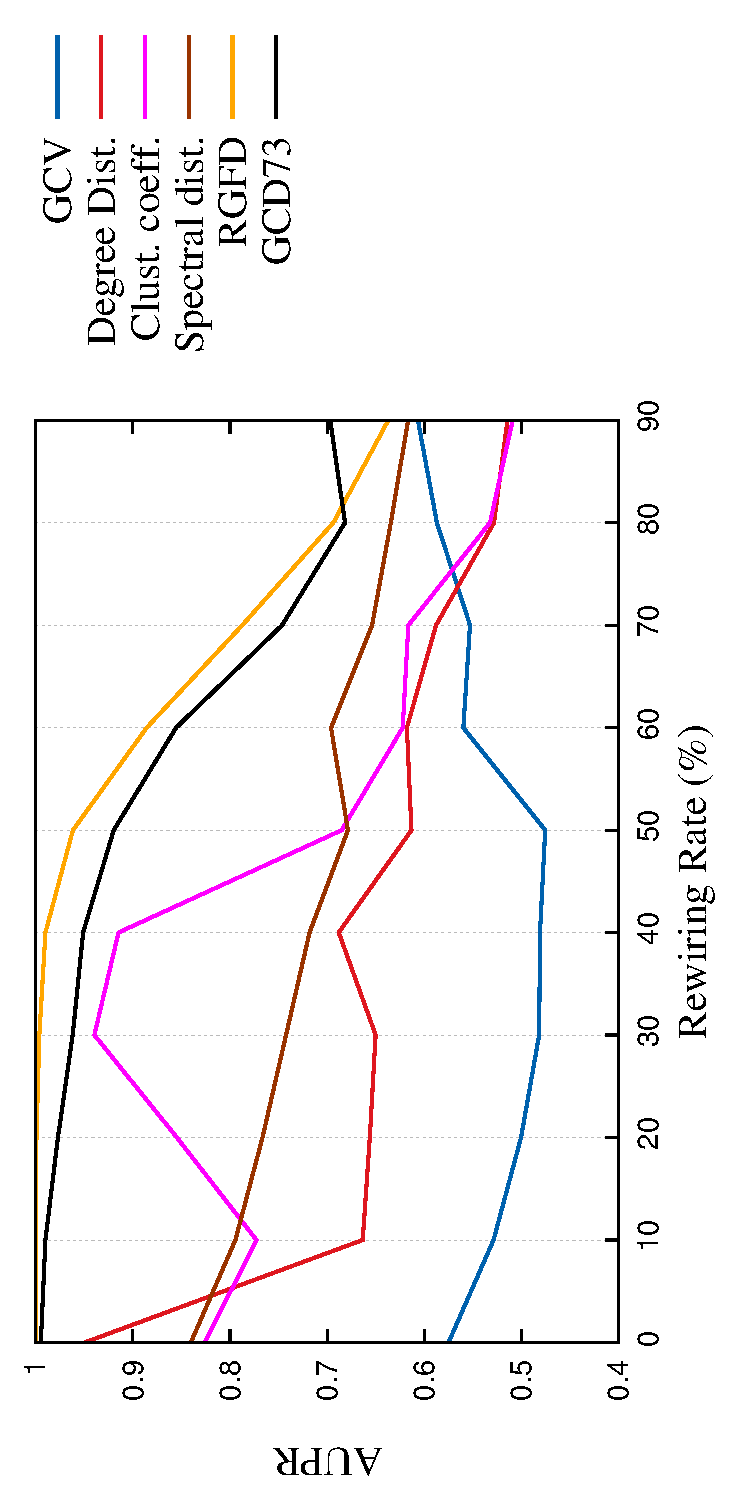
\includegraphics[scale=0.7, angle=-90]
  {../code/final_results/trade_2010_thresholded/eval_results/rew_aupr_all_sigs2.pdf}
  \caption[The AUPR for different percentages of noise in the model networks]{The AUPR for different percentages of noise in the model networks. The rewiring probability increases from 0 to 90\%. The GCV signature has a poor performance when dealing with noisy data, having the lowest AUPR when the rewiring parameter is in the [0--70] range.}
  \label{fig:rew_aupr}
\end{figure}

\subsection{Edge completeness}

In real-life situations, one also has to deal with incomplete data. In order to simulate incomplete data in our networks, we remove $q\%$ of the edges from the networks, where $q$ varies from 100\% (full network) to 10\% (incomplete network). Moreover, in order to simulate both noisy and incomplete data, we choose the 40\% rewired networks as the starting point and then start removing edges from these networks. We evaluate the performance of the signatures on these noisy and incomplete networks. 

\hilight{fix the p and q percentages fonts}

Figure \ref{fig:compl_aupr} shows the AUPR of the networks as the edge completeness parameter varies from 100\% to 10\%. The initial networks have been rewired with a 40\% probability. All the signatures display a general downward trend. The GCV signature performs poorly also in this experiment, always having an AUPR that is smaller than the AUPR of the other signatures. Some signatures such as the RGFD have a sharper drop in their AUPR than other signatures such as the Spectral Distribution. This suggests that RGFD is not as robust to incomplete data as the Spectral Distribution is. We conclude that the GCV signature is unable to deal with incomplete data either.

\begin{figure}[H]
  \hspace{-1.5em}
  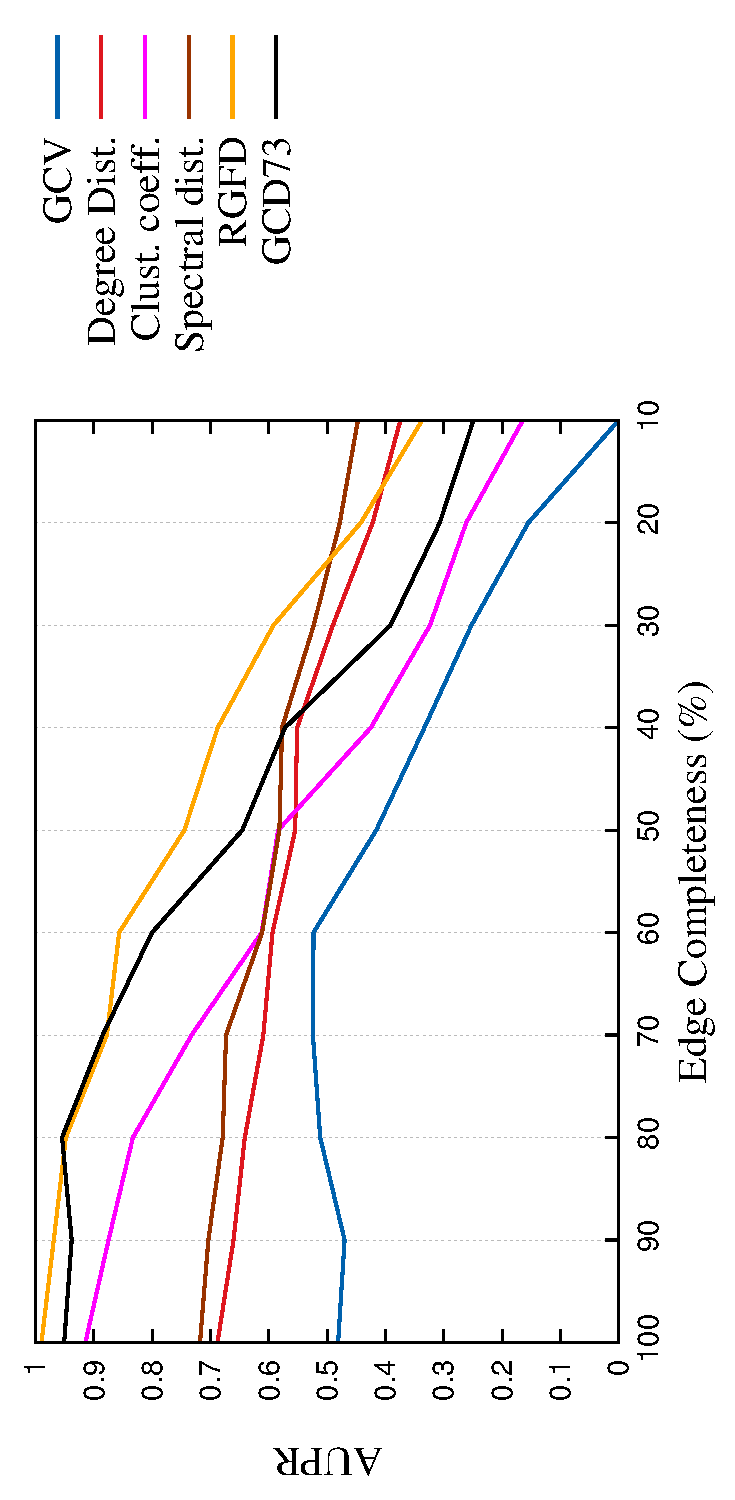
\includegraphics[scale=0.7, angle=-90]
  {../code/final_results/trade_2010_thresholded/eval_results/compl_aupr_all_sigs2.pdf}
  \caption[The AUPR for different percentages of edge completeness in the model networks]{The AUPR for different percentages of edge completeness in the model networks. The GCV signature also has a poor performance when dealing with incomplete data, always having the lowest AUPR compared to the other signatures.}
  \label{fig:compl_aupr}
\end{figure}

\subsection{Signature approximation}

In order to speed up computation, sometimes we have to approximate the signatures that are computed for all the random networks. In this section we try to evaluate the robustness of each signature to approximation. For each network, we only use a percentage $p\%$ of nodes to calculate the signatures. This is done for each signature/metric in the following manner:
\begin{enumerate}
 \item Graphlet Cluster Vector (GCV): We compute the Pearson's GCV correlation matrix using the GCV signatures of only $p\%$ of the nodes.
 \item Degree Distribution: We calculate the degree distribution from $p\%$ of the nodes in the graph.
 \item Average clustering coefficient: We average only the clustering coefficient of $p\%$ of the nodes.
 \item Spectral distribution: We compute the Laplacian matrix $L$ of the original network, then randomly sample $p\%$ nodes and take the submatrix $L'$ of $L$ that corresponds to the sampled nodes. We compute the spectral distribution from the submatrix $L'$.
 \item Graphlet Frequency Vector (used for computing RGFD): We randomly sample $p\%$ of the nodes and take the induced subgraph $S$ on these nodes. We then compute the GFV in $S$.
 \item GCD73: We compute the Graphlet correlation matrices using the GDV signatures of only $p\%$ of the nodes.  
\end{enumerate}

The experiments for signature approximation have also been run using the 40\% rewired networks, which simulate noisy data. The results are presented in figure \ref{fig:sampl_aupr}. For the GCV signature, we notice that it is actually robust to signature approximation, showing a very small but steady drop in the AUPR as less nodes are sampled. Other metrics such as the RGFD show a sharp drop in AUPR from 1.0 to 0.2, suggesting that RGFD is not robust to approximations. The Spectral distribution can also be considered robust, showing a peak AUPR of 0.7 when 50\% of the nodes are sampled. 

\begin{figure}[H]
  \hspace{-1.5em}
  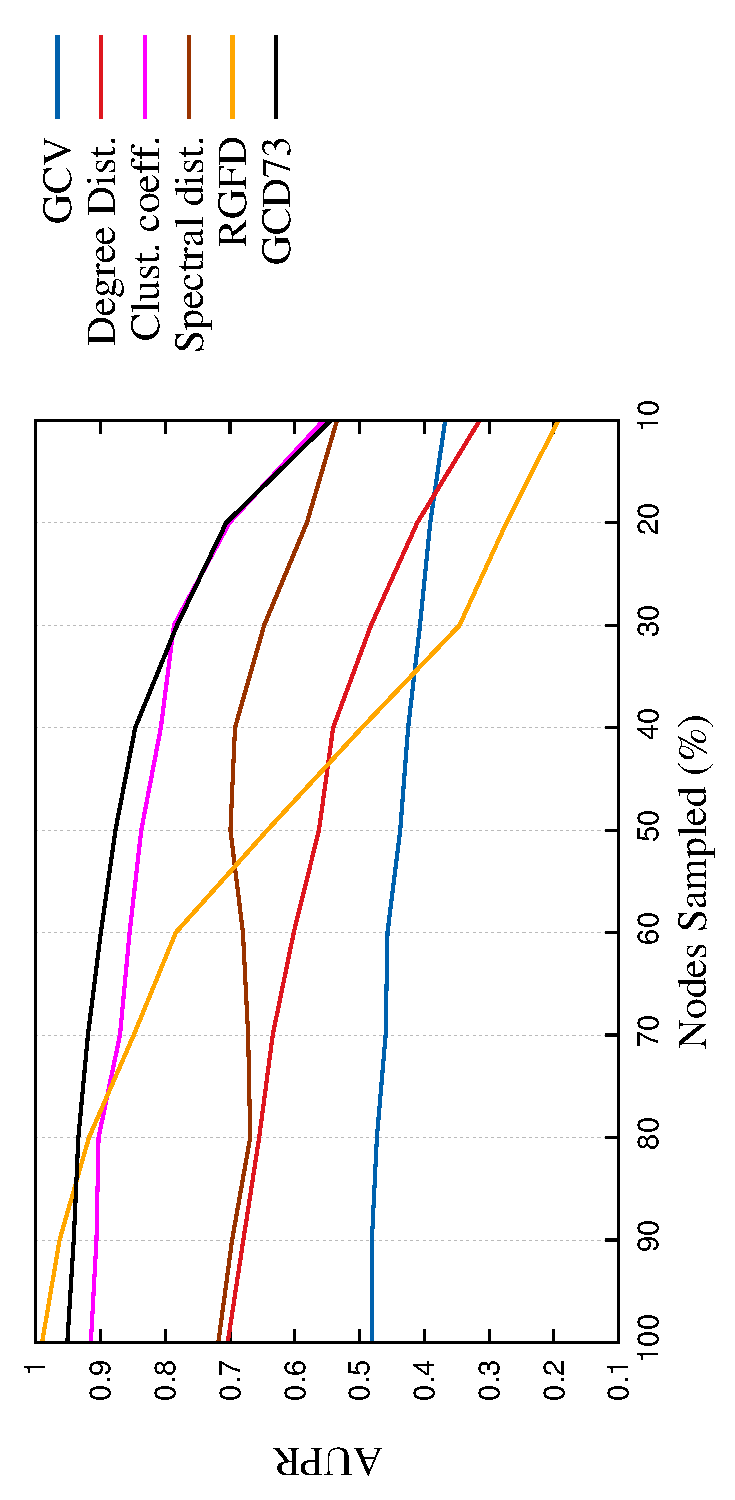
\includegraphics[scale=0.7, angle=-90]
  {../code/final_results/trade_2010_thresholded/eval_results/sampl_aupr_all_sigs2.pdf}
  \caption[The AUPR for different percentages of nodes sampled in the model networks]{The AUPR for different percentages of nodes sampled in the model networks. The GCV signature is robust to approximation, showing only a slight but steady drop in AUPR as the percentage of nodes sampled varies from 100\% to 10\%. On the other hand, the RGFD shows a sharp drop, suggesting that it is not robust to signature approximation.}
  \label{fig:sampl_aupr}
\end{figure}

In conclusion, the novel GCV signature is not robust to noisy or incomplete data, but it is robust to signature approximation. The signatures that performed best on our tests are the RGFD and GCD73, which are mostly robust to noisy and incomplete data.

\section{GCV-based Classifier}
\label{sec:eval_classify}

In this section we evaluate the performance of the GCV signature at classifying proteins into functional classes. We use Collin's Yeast AP-MS PPI network for computing the GCV of each protein.\footnote{The reason we run it on Collin's AP-MS network is because CCA analysis has given a high correlation on this dataset (see section \ref{sec:18_ppi_cca_results}).} Separately, we label each protein using Boone's annotation that comprises 14 different classes. The classifier we wrote uses a K-nearest neighbours (K-NN) method for predicting the function of a protein in the following manner:
\begin{itemize}
 \item Compute the GCV signature for all the proteins in the input network.
 \item For predicting the function of a given protein, compute the Euclidean distances between the GCV of the protein and the GCV of all the other proteins in the training data set. Store the distances in an array and sort it. 
 \item Find the closest $K$ data points to the input protein according to the computed distances.
 \item Perform majority voting\footnote{In majority voting, the class that has the highest frequency is the one that is returned. If two or more classes have the same highest frequency, one of them is chosen at random.} on the classes of the $K$ nearest neighbours and return the result as the predicted class.
\end{itemize}

This process is run inside a Cross-validation framework, where the protein dataset is split into two groups:
\begin{itemize}
 \item training data: this is stored in a data structure and is used for predicting the class of proteins using K-NN
 \item test data: this dataset is used for the actual prediction.
\end{itemize}

We split the dataset into 10 different chunks and run 10-fold cross-validation. We also choose $N = 5$ as the number of neighbours on which majority voting is performed. At each fold, 90\% of the data is used for training and 10\% for testing. For each fold during cross-validation, we compute a confusion matrix $M$ for all the classes, where entry $M(i,j)$ corresponds to the number of data points that have actual label $i$, but the classifier predicted them as having label $j$. The confusion matrices for each fold are added together and a final confusion matrix is obtained at the end of the cross-validation process. From the final confusion matrix, we then count for each class $C$ the following types of data points:
 \begin{itemize}
  \item \textbf{True Positives} ($TP$) are the data points that belong to $C$ and have also been correctly predicted as belonging to class $C$.
  \item \textbf{False Positives} ($FP$) the data points that do not belong to $C$ but have been incorrectly predicted as belonging to class $C$.
  \item \textbf{True Negatives} ($TN$) are the data points that not belong to $C$ and have also been correctly predicted as not belonging to class $C$.
  \item \textbf{False Negatives} ($FP$) the data points that do not belong to $C$ but have been incorrectly predicted as belonging to class $C$.
 \end{itemize}

After we compute the number of $TP$, $FP$, $TN$ and $FN$ data points, we can calculate for each class $C$ the following 3 statistics:
\begin{itemize}
 \item Precision: the percentage of data points that have been correctly classified in $C$ out of all the data points that have been classified in $C$. The exact formula for precision is:
 $$ Precision = \frac{TP}{TP + FP}$$
  \item Recall: the percentage of data points that have been correctly classified in $C$ out of all the data points are in $C$. It is formally defined as:
 $$ Recall = \frac{TP}{TP + FN}$$
  \item $F_1$ score: it is a measure of the test's accuracy that combines both precision and recall. The formula for $F_1$ is as follows:
 $$ F_1 = \frac{2 * Precision * Recall}{Precision + Recall}$$
 
\end{itemize}

\subsection{Classifier Results}

\definecolor{header}{HTML}{9DE6E6} % 
\definecolor{diag}{HTML}{05D1FF} % 

Figure \ref{fig:conf_matrix} shows the confusion matrix obtained for Collin's AP-MS Yeast PPI network using Boone's annotations. Note that only part of the classes have been tested in our classifier. The reason for this is because there were not enough data points for some classes to allow our algorithm to run properly. For example, there was only one sample belonging to the class \emph{Cell cycle progression/meiosis} in our dataset. As a result, we ran our classifier only on 9 classes that did not originally give an $F_1$ score of zero.\footnote{We first ran our classifier using all the classes and removed the classes for which the final $F_1$ score was zero.}

We observe that although our classifier correctly classified some data points (diagonal entries), there are considerable errors, especially in the first column (Nuclear transport). A considerable number of data entries have been incorrectly predicted as belonging to Nuclear transport, and we attribute this to the following bias in our methodology: during the majority voting phase, if two or more frequencies have the same highest score, the class with the lowest index is ultimately selected. As a result, the first class (Nuclear transport) is more likely to be selected as 
opposed to others. A closer look at the data further explains why some of the proteins are wrongly classified: there are many proteins that have the exact same GCV signature but different functional annotations. Most of these proteins tend to have a sparse neighbourhood, a fact that is easily noticed in the GCV signature, with many frequencies set to zero. 

On the other hand, we also notice that there is a large number of True Positives for RNA processing (RNA proc.), Chromatin transcription (Chrom. transc.) and Ribosome translation (Rib. transl.). Ribosome Translation and Chromatin transcription also had a large cross-loading magnitude in the CCA analysis (see figure \ref{yeast_apms_collins_cca}). We can therefore conclude that the GCV signature is particularly suitable for analysing proteins that are involved in Ribosome translation and Chromatin transcription.

Finally, the classifier has not correctly classified any protein labelled with DNA replication, as there are no True Positives for this class. The reason for this might be because we only use $N = 5$ nearest neighbours, and if the classifier finds at least 3 proteins from Nuclear Transport (Nucl. trans.) that have the same GCV signature as a protein that belongs to DNA replication, it will instead be assigned a Nuclear Transport label instead. We have tried using a value of $K$ that is bigger than 5, but that did not result in a better classification, having the final $F_1$ score approximately the same or lower.

\begin{figure}[H]
\centering
\begin{tabular}{p{2.7cm} p{1.0cm} p{1.0cm} p{1.0cm} p{1.0cm} p{1.0cm} p{1.0cm} p{1.0cm} p{1.0cm} p{1.0cm} }
\cellcolor{header} \backslashbox{actual}{pred.}  & \cellcolor{header} Nucl. trans.  & \cellcolor{header} Chrom. seg.  & \cellcolor{header} RNA proc.  & \cellcolor{header} Chrom. transc.  & \cellcolor{header} DNA repl.  & \cellcolor{header} Prot. deg.  & \cellcolor{header} Golgi sort.  & \cellcolor{header} Metab.  & \cellcolor{header} Rib. transl. \\

\cellcolor{header} Nucl. trans. &  \cellcolor{diag}  24 &  3 &  5 &  2 &  0 &  0 &  4 &  1 &  1\\ 

\cellcolor{header} Chrom. seg. &  41 &  \cellcolor{diag}  23 &  5 &  3 &  0 &  3 &  1 &  0 &  1\\ 

\cellcolor{header} RNA proc. &  42 &  11 &  \cellcolor{diag}  99 &  26 &  0 &  5 &  7 &  1 &  18\\ 

\cellcolor{header} Chrom. transc. &  62 &  21 &  20 &  \cellcolor{diag}  95 &  0 &  6 &  6 &  1 &  11\\ 

\cellcolor{header} DNA repl. &  67 &  10 &  1 &  3 &  \cellcolor{diag}  0 &  0 &  1 &  1 &  1\\ 

\cellcolor{header} Prot. deg. &  19 &  5 &  3 &  6 &  0 &  \cellcolor{diag}  18 &  0 &  0 &  0\\ 

\cellcolor{header} Golgi sort. &  63 &  21 &  2 &  13 &  0 &  0 &  \cellcolor{diag}  23 &  0 &  0\\ 

\cellcolor{header} Metab. &  72 &  4 &  4 &  2 &  0 &  0 &  2 &  \cellcolor{diag}  7 &  4\\ 

\cellcolor{header} Rib. transl. &  35 &  10 &  31 &  23 &  0 &  0 &  0 &  1 &  \cellcolor{diag}  60\\ 

\end{tabular}
\caption[Confusion matrix obtained on Collins AP-MS Yeast PPI network after 10-fold cross-validation.]{Confusion matrix obtained on Collins AP-MS Yeast PPI network after 10-fold cross-validation, using Boone's annotations as classes. The rows represent actual classes, while columns represent predicted classes. The classes used were: Nuclear transport (Nucl. trans.), Chromatin segmentation (Chrom. seg.), RNA processing (RNA proc.), Chromatin transcription (Chrom. transc.), DNA replication, repair, HR cohesion (DNA repl.), Protein degradation (Prot. deg.), Golgi endosome vacuole sorting (Golgi sort.), Metabolism - mitochondria (Metab.) and Ribosome translation (Rib. transl).}
\label{fig:conf_matrix}
\end{figure}

Table \ref{tab:prec_rec_f1_table} shows the Precision, Recall and $F_1$ rates for each of the 9 classes used by our classifier. At the bottom of the table, the average precision, recall and $F_1$ rates across all classes are shown. The results in the table show that the GCV-based classifier is not efficient at classifying proteins according to their function. The average precision and recall rates are only 0.41 and 0.31 respectively, while the average $F_1$ rate is 0.29. However, there is considerable variance in precision, recall and $F_1$ rates across the classes. For example, the classifier has a relatively high precision for classes such as Ribosome translation, Protein degradation, Golgi Endosome sorting and RNA processing. On the other hand, a class such as DNA replication has zero precision, meaning that no protein has been correctly classified to this class.

Overall, we conclude that the GCV-based K-NN classifier is not suitable for labelling proteins from PPI networks according to their function. Nevertheless, it still performs 3-4 times better than a random classifier, which would have average precision, recall and $F_1$ rates of around $\frac{1}{9} = 0.11$, when 9 classes are used. Last but not least, we also tried running the same classifier with different parameters $N$ -- nearest neighbours and $F$ -- fold numbers. When varying $N$, we got the best results when $N$ was in the range [5,10], although the performance decreases only slightly for $N$ greater than 10.

\begin{table}[H]
  \centering
  \begin{tabular}{  c | c  c  c }
    Class & Precision & Recall & F1\\
    \hline
    Nuclear-cytoplasmic transport & 0.056 & 0.600 & 0.103\\
    Chromatin segmentation  & 0.213 & 0.299 & 0.249\\
    RNA processing & 0.582 & 0.474 & 0.522\\
    Chromatin transcription & 0.549 & 0.428 & 0.481\\
    DNA replication, repair, HR cohesion & 0.000 & 0.000 & 0.000\\
    Protein degradation proteosome & 0.562 & 0.353 & 0.434\\
    Golgi endosome vacuole sorting & 0.523 & 0.189 & 0.277\\
    Metabolism - mitochondria & 0.583 & 0.074 & 0.131\\
    Ribosome translation & 0.625 & 0.375 & 0.469\\
    \hline
    Average & 0.410 & 0.310 & 0.296\\
  \end{tabular}
  \caption[Precision, recall and $F_1$ rates for each class used by the protein annotation classifier.]{Precision, recall and $F_1$ rates for each class used by the protein annotation classifier. At the bottom of the table, the overall average precision, recall and $F_1$ rates are given. The low scores in average precision (0.41), recall (0.31) and $F_1$ (0.29) suggest that our GCV-based classifier is not suitable for classifying proteins according to their function.}
  \label{tab:prec_rec_f1_table}
\end{table}

\section{Evaluation Summary}

We conclude that when clustering random networks generated with different algorithms, the GCV signature is not as efficient as other signatures or metrics. Nevertheless, the GCV can still be successfully used for data analysis and it helped us uncover interesting insights from the economic and biological networks. Moreover, the GCV might still be successfully used for clustering, if combined with other signatures such as the GDV.

Furthermore, our results do not precisely resemble those obtained by Yavero\u{g}lu et al. in 2014 \cite{yaverouglu2014revealing}. The reason for this is because we have not used the same source network to generate the random networks. Moreover, Yavero\u{g}lu et al. have also done the precision-recall curve analysis on a larger number of networks. In our case, we considered that 150 generated networks are sufficient to perform the analysis and draw our conclusions.

Section \ref{sec:eval_classify} also showed that the GCV signature cannot be directly used as a classifier without further modifications. The K-NN classifier we built for Collin's AP-MS Yeast PPI network using Boone's annotations is not precise and has a low $F_1$ score of 0.29. The reason for this is because there are several proteins that have the exact same GCV signature but different functional labels. We therefore suggest an improved GCV signature that captures more information about the protein's neighbourhood. One possibility is the combination of GDV and GCV signatures into one vector of frequencies. 



% Chapter 6
\chapter{Conclusion}

% Summary of achievements and Future work

This interim report offers a clear perspective on the work done on this project
so far. I have successfully developed the mathematical model for the GCV
signature and I have implemented in an efficient manner the core algorithms
necessary for the project. I have also performed some early experiments that
showed some interesting properties of the metric. 

Nonetheless, I also encountered several problems that I could not really
foresee, which delayed the usual progress of the project. For instance, right
at the very beginning I when I was working on the mathematical model, I could
not mathematically find what the maximum possible number of graphlets of a
particular type in a graph of N nodes. After I finished the mathematical model,
I also had to spend some time reformatting the graphlet counting function that I
was given. Although it took me a while to solve these tasks, I believe it was
good that I tackled them in this manner, as it helped me better understand the
nature of the project I was working on, both from a mathematical and a
computational perspective.
 
\section{Future work}

As I have previously mentioned, our future work mainly consists in performing
more experiments with the GCV signature in order to find out its properties.
Our group is fairly confident that we will get a lot of interesting results. We
are therefore planning to publish one paper with these results in a
Bioinformatics journal.

One other idea we could explore is to try to derive several related metrics
using different normalisation procedures or even combine the GCV with the older
GDV metric. This could allow us to effectively use the power of both metrics at
the same time. 

Another idea that I had while discussing with Zoran, one of Dr. Przulj's
collaborators, was to find out how important each of the elements from the
\emph{Graphlet Cluster Vector} was by assigning a weight to each of them. Using
some machine learning techniques or linear regression, some optimal weights
could be derived which would make the signatures more efficient when comparing
them with each other or when calculating the \emph{Relative Cluster Frequency
Distance}. Unfortunately, these tasks are outside the scope of our project, as
they can take a few months to complete and I wouldn't have enough time to finish
them by July. 

Finally, we hope that our work will help us better understand local properties
of biological or economic networks and that it will make an impact in the
Bioinformatics community. Ultimately, network analysis is a never-ending task:
one can always find better ways to explain phenomena or behaviour, and even
more, as this phenomena or behaviour changes over time, new models need to be
developed that model then as closely as possible.



\nocite{*} % Show all Bib-entries
\bibliographystyle{unsrt}
\bibliography{gcv}



\appendix
% these do NOT count as part of the suggested page count
% This is probably a good place to explain the models in some detail for example

\chapter{Statistical results}


\begin{figure}[H]
  \centering
\includegraphics[angle=-90,scale=0.6]
{../code/extra_results/saudi_oil/saudi_orig_gcv_oil2}
\caption[The change in the un-normalised GCV of Saudi Arabia along with the change in Crude Oil price.]{The change in the un-normalised GCV of Saudi Arabia along with the change in Crude Oil price. The un-normalised GCV is not suitable for correlating the GCV of Saudi Arabia with the change in crude oil price, because Spearman's rank correlation coefficient is small (less than 0.13), while the p-value is large (bigger than 0.35). This is the case for all shifts in GCV in the range $[-2,2]$}
\label{saudi_oil_orig}
\end{figure}

\chapter{Canonical Correlation Tables}


\definecolor{col1}{HTML}{5752FF} % blue
\definecolor{col2}{HTML}{05D1FF} % 
\definecolor{col3}{HTML}{85FFA3} % 
\definecolor{col4}{HTML}{C8FF85} % 
\definecolor{col5}{HTML}{F5FF85} % 
\definecolor{col6}{HTML}{FFA985} % 
\definecolor{col7}{HTML}{FF8585} % red



\begin{figure}[H]
  \begin{subfigure}{.7\textwidth}
  \centering
  \begin{tabular}{ c c | c c }
    \multicolumn{2}{c}{Canonical Correlation} &  \multicolumn{2}{c}{0.89595} \\
    \multicolumn{2}{c}{p-value} &  \multicolumn{2}{c}{0.00000} \\
    \hline
    \multicolumn{2}{c}{X variate} & \multicolumn{2}{c}{Y variate}\\
    \hline
  POP & 0.76667 &  G1 & 0.82332\\
  LE & 0.75818 &  G2 & 0.80569\\
  KIxRGDPLxPOP & 0.72552 &  G6 & 0.80315\\
  RGDPCHxPOP & 0.71889 &  G7 & 0.79365\\
  RGDPLxPOP & 0.71877 &  G3 & 0.78361\\
  RGDPL2xPOP & 0.71683 &  G4 & 0.78270\\
  KCxRGDPLxPOP & 0.69962 &  G17 & 0.77813\\
  KGxRGDPLxPOP & 0.69344 &  G22 & 0.76781\\
  KCxRGDPL & 0.42077 &  G23 & 0.76656\\
  RGDPCH & 0.26634 &  G24 & 0.76458\\
  RGDPL & 0.26629 &  G14 & 0.76293\\
  RGDPL2 & 0.26616 &  G26 & 0.75734\\
  KGxRGDPL & 0.21884 &  G8 & 0.75020\\
  KIxRGDPL & 0.17869 &  G13 & 0.74857\\
  XRAT & 0.11999 &  G19 & 0.74581\\
  KC & 0.09780 &  G28 & 0.74525\\
  KI & -0.05999 &  G18 & 0.74056\\
  BCAperRGDPL & -0.14775 &  G12 & 0.74053\\
  KG & -0.17422 &  G11 & 0.73369\\
  BCA & -0.20019 &  G10 & 0.72915\\
  OPENK & -0.24745 &  G9 & 0.72424\\
  & &  G27 & 0.70899\\
  & &  G29 & 0.68727\\
  & &  G21 & 0.67142\\
  & &  G5 & 0.66142\\
  & &  G25 & 0.63754\\
  & &  G16 & 0.62203\\
  & &  G15 & 0.57546\\
  & &  G20 & 0.44454\\
  \end{tabular}
  \end{subfigure}
  \begin{subfigure}{.25\textwidth}
    \centering 
    \rowcolors{1}{}{}		
    
    \gone
    \gtwo
    \gsix
    \gdots
    \gsixteen
    \gfifteen
    \gtwenty
    
  \end{subfigure}
  
  \caption[CCA - World Trade Network - unnormalised GCV]{Canonical Correlation Analysis between economic indicators ($X$ variate) and the unnormalised GCV signature ($Y$ variate) on the 2010 World Trade network. Openness (OPENK), Balance Current Account (BCA) a few other indicators correlate negatively with all the graphlets, because their cross-loadings have different signs. On the other hand, the rest of the indicators such as Population (POP), Level of Employment (LE) and GDP per capita (RGPDL, RGDPCH) correlate positively with all the graphlets, since their cross-loadings have the same sign. The overall correlation is 0.89 with a p-value of 0.0. In reality, the p-value is extremely small but it has been truncated to zero because of floating point approximations.}
  \label{all_trade_thresh_cca_orig}
\end{figure}




\begin{figure}[H]
  \begin{subfigure}{.65\textwidth}
  \centering
  \begin{tabular}{ c c | c c }
    \multicolumn{2}{c}{Canonical Correlation} &  \multicolumn{2}{c}{0.94594} \\
    \multicolumn{2}{c}{p-value} &  \multicolumn{2}{c}{0.00000} \\
    \hline
    \multicolumn{2}{c}{X variate} & \multicolumn{2}{c}{Y variate}\\
    \hline
  POP & 0.73628 &  \cellcolor{col2} G12 & 0.90456\\
  LE & 0.71650 &  \cellcolor{col1} G10 & 0.89337\\
  KI x RGDPL x POP & 0.66038 &  \cellcolor{col2}G14 & 0.87536\\
  RGDPCH x POP & 0.65383 &  \cellcolor{col3}G17 & 0.85955\\
  RGDPL x POP & 0.65376 &  \cellcolor{col1}G9 & 0.84692\\
  RGDPL2 x POP & 0.65226 &  \cellcolor{col1}G11 & 0.83708\\
  KG x RGDPL x POP & 0.64238 &  \cellcolor{col3}G19 & 0.70966\\
  KC x RGDPL x POP & 0.63303 &  \cellcolor{col1}G4 & 0.69198\\
  KC x RGDPL & 0.29252 &  \cellcolor{col2}G16 & 0.67490\\
  XRAT & 0.17083 &  \cellcolor{col1}G3 & 0.63019\\
  RGDPCH & 0.16079 &  \cellcolor{col3}G18 & 0.60564\\
  RGDPL & 0.16071 &  \cellcolor{col4}G24 & 0.59760\\
  RGDPL2 & 0.16038 &  \cellcolor{col2}G13 & 0.59247\\
  KG x RGDPL & 0.15848 &  \cellcolor{col4}G22 & 0.54531\\
  KI x RGDPL & 0.10411 &  \cellcolor{col4}G23 & 0.47154\\
  KC & 0.08634 &  \cellcolor{col2}G15 & 0.43876\\
  KI & -0.01620 &  \cellcolor{col3}G21 & 0.32221\\
  BCA per RGDPL & -0.10953 &  \cellcolor{col3}G20 & 0.28966\\
  KG & -0.12868 &  \cellcolor{col5}G26 & 0.27068\\
  BCA & -0.14935 &  \cellcolor{col3}G6 & 0.23057\\
  OPENK & -0.26502 &  \cellcolor{col5}G27 & 0.15386\\
  & &  \cellcolor{col4}G25 & 0.14823\\
  & &  \cellcolor{col3}G5 & 0.11232\\
  & &  \cellcolor{col6}G28 & -0.15016\\
  & &  \cellcolor{col5}G1 & -0.16367\\
  & &  \cellcolor{col6}G7 & -0.21277\\
  & &  \cellcolor{col7}G2 & -0.48656\\
  & &  \cellcolor{col7}G29 & -0.52462\\
  & &  \cellcolor{col7}G8 & -0.63741\\
  \end{tabular}

  \end{subfigure}
  \begin{subfigure}{.25\textwidth}
    \centering 
    \rowcolors{1}{}{}		
	
    \gtwelve
    \gten
    \gfourteen
    \gdots
    \gtwo
    \gtwentynine
    \geight

  \end{subfigure}
  
\caption[CCA - World Trade networks - normalised GCV]{CCA between the economic indicators and the normalised GCV signature on the 2010 World Trade network. Each graphlet has been colour-coded according to its density, from sparse graphlets in blue to dense graphlets and cliques in red. One can notice how the sparse graphlets have a positive cross-loading, while the dense graphlets have a negative cross-loading. Sparse graphlets are correlated with good economic indicators such as Population (POP), Level of Employment (LE) and GDP per Capita (RGDPL), while dense graphlets are correlated with bad indicators such as the Balance of Current Account (BCA).\hilight{Add a bar showing what the colours mean}}
\label{all_trade_thresh_cca}
\end{figure}


\begin{figure}
  \begin{subfigure}{.65\textwidth}
  \centering
  \begin{tabular}{ c c | c c }
    \multicolumn{2}{c}{Canonical Correlation} &  \multicolumn{2}{c}{0.53013} \\
    \multicolumn{2}{c}{p-value} &  \multicolumn{2}{c}{0.00000} \\
    \hline
    \multicolumn{2}{c}{X variate} & \multicolumn{2}{c}{Y variate}\\
    \hline
  Ribosome translation & 0.91618 &  G2 & 0.89916\\
  RNA processing & 0.08561 &  G8 & 0.86246\\
  Protein degredation  & -0.01381 &  G29 & 0.83575\\
  Cell cycle & -0.01819 &  G7 & 0.81776\\
  Nuclear cytoplasmic transport & -0.07635 &  G1 & 0.81549\\
  ER Golgi traffic & -0.10132 &  G28 & 0.79973\\
  Protein folding & -0.10205 &  G26 & 0.76710\\
  Chromatin  segmentation & -0.12005 &  G27 & 0.75955\\
  Signaling stress response & -0.12897 &  G5 & 0.74980\\
  Cell polarity morphogenesis & -0.14394 &  G6 & 0.73719\\
  Chromatin transcription & -0.14560 &  G22 & 0.72618\\
  DNA replication & -0.17095 &  G24 & 0.71387\\
  Metabolism mitochondria & -0.17109 &  G25 & 0.70796\\
  Golgi endosome vacuole sorting & -0.20098 &  G23 & 0.67823\\
  & &  G4 & 0.65612\\
  & &  G20 & 0.65406\\
  & &  G17 & 0.63899\\
  & &  G21 & 0.61750\\
  & &  G19 & 0.59378\\
  & &  G3 & 0.59369\\
  & &  G16 & 0.54884\\
  & &  G14 & 0.54406\\
  & &  G18 & 0.53288\\
  & &  G15 & 0.52898\\
  & &  G12 & 0.52683\\
  & &  G11 & 0.49169\\
  & &  G13 & 0.41908\\
  & &  G10 & 0.41706\\
  & &  G9 & 0.38194\\

  \end{tabular}

  \end{subfigure}
  \begin{subfigure}{.25\textwidth}
    \centering 
    \rowcolors{1}{}{}		
	
	
    \gtwo
    \geight
    \gtwentynine
    \gdots
    \gthirteen
    \gten
    \gnine
    
    
    


  \end{subfigure}
  
\caption[CCA Analysis on Collin's AP-MS Yeast PPI network.]{CCA Analysis on Collin's AP-MS Yeast PPI network. The $X$ variate is represented by Boone's protein annotations (see section \ref{ppi_annotations}), while the $Y$ variate is represented by the GCV signature. The correlation value is 0.53 and the p-value is shown as 0.0 due to floating point approximations, although in reality it is very low but not exactly 0.0. RNA processing and Ribosome translation correlate positively with all the graphlets because their weights have the same sign, while the rest of the protein annotations correlate negatively with all the graphlets.}
\label{yeast_apms_collins_cca}
\end{figure}


\section{The 17 experiments}

In this section we only show the results that were statistically significant. All the other results can be found in the source code under \lstinline|final_results/all_ppi/|


% ./6-yeast_apms_collins_boone_CCA/CCA_out/yeast_apms_collins.txt

% \begin{figure}[H]
% \centering
% \begin{tabular}{ c c | c c }
%   \multicolumn{2}{c}{Canonical Correlation} &  \multicolumn{2}{c}{0.53013} \\
%   \multicolumn{2}{c}{p-value} &  \multicolumn{2}{c}{0.00000} \\
%   \hline
%   \multicolumn{2}{c}{X variate} & \multicolumn{2}{c}{Y variate}\\
%   \hline
%  Golgi endosome vacuole sorting & 0.11166 &  G9 & -0.21219\\
%  Metabolism mitochondria & 0.09505 &  G10 & -0.23170\\
%  DNA replication   repair HR cohesion & 0.09497 &  G13 & -0.23282\\
%  Chromatin transcription & 0.08089 &  G11 & -0.27316\\
%  Cell polarity morphogenesis & 0.07997 &  G12 & -0.29269\\
%  Signaling stress response & 0.07165 &  G15 & -0.29388\\
%  Chrom  seg  kinetoch  spindle microtub  & 0.06670 &  G18 & -0.29605\\
%  Protein folding   glycosylation cell wall & 0.05669 &  G14 & -0.30226\\
%  ER Golgi traffic & 0.05629 &  G16 & -0.30491\\
%  Nuclear cytoplasmic transport & 0.04242 &  G3 & -0.32983\\
%  Cell cycle progression meiosis & 0.01010 &  G19 & -0.32988\\
%  Protein degredation proteosome & 0.00767 &  G21 & -0.34306\\
%  RNA processing & -0.04756 &  G17 & -0.35499\\
%  Ribosome translation & -0.50899 &  G20 & -0.36336\\
%  & &  G4 & -0.36451\\
%  & &  G23 & -0.37679\\
%  & &  G25 & -0.39331\\
%  & &  G24 & -0.39659\\
%  & &  G22 & -0.40344\\
%  & &  G6 & -0.40955\\
%  & &  G5 & -0.41656\\
%  & &  G27 & -0.42197\\
%  & &  G26 & -0.42617\\
%  & &  G28 & -0.44430\\
%  & &  G1 & -0.45305\\
%  & &  G7 & -0.45431\\
%  & &  G29 & -0.46431\\
%  & &  G8 & -0.47914\\
%  & &  G2 & -0.49953\\
% \end{tabular}
% \caption[CCA Analysis on Collin's AP-MS Yeast PPI network  -- Boone's annotations]{CCA Analysis on Collin's AP-MS Yeast PPI network \cite{collins2007toward}. The $X$ variate is represented by Boone's protein annotations (see section \ref{ppi_annotations}), while the $Y$ variate is represented by the GCV signature. The correlation value is 0.53 and the p-value is shown as 0.0 due to floating point approximations, although in reality it is very low but not exactly 0.0. RNA processing and Ribosome translation correlate positively with all the graphlets because their weights have the same sign, while the rest of the protein annotations correlate negatively with all the graphlets.}
% \label{all_ppi6}
% \end{figure}


% ./7-yeast_biogrid_genetic_boone_CCA/CCA_out/yeast_biogrid_genetic.txt


\begin{figure}[H]
\centering
\begin{tabular}{ c c | c c }
  \multicolumn{2}{c}{Canonical Correlation} &  \multicolumn{2}{c}{0.34590} \\
  \multicolumn{2}{c}{p-value} &  \multicolumn{2}{c}{0.00000} \\
  \hline
  \multicolumn{2}{c}{X variate} & \multicolumn{2}{c}{Y variate}\\
  \hline
 Metabolism mitochondria & 0.14787 &  G11 & -0.05518\\
 Ribosome translation & 0.07535 &  G10 & -0.08810\\
 Cell polarity morphogenesis & 0.05944 &  G9 & -0.09217\\
 RNA processing & 0.05671 &  G14 & -0.10260\\
 Protein folding   glycosylation cell wall & 0.04637 &  G16 & -0.11486\\
 Signaling stress response & 0.04030 &  G13 & -0.11736\\
 Cell cycle progression meiosis & 0.03541 &  G12 & -0.11781\\
 Nuclear cytoplasmic transport & 0.01806 &  G15 & -0.11783\\
 Golgi endosome vacuole sorting & 0.01673 &  G4 & -0.12001\\
 Protein degredation proteosome & -0.00325 &  G3 & -0.13304\\
 ER Golgi traffic & -0.01553 &  G20 & -0.13733\\
 Chrom  seg  kinetoch  spindle microtub  & -0.03107 &  G18 & -0.13930\\
 DNA replication   repair HR cohesion & -0.21915 &  G17 & -0.13935\\
 Chromatin transcription & -0.23242 &  G21 & -0.14204\\
 & &  G19 & -0.14416\\
 & &  G25 & -0.16429\\
 & &  G5 & -0.16538\\
 & &  G22 & -0.16542\\
 & &  G24 & -0.16634\\
 & &  G6 & -0.16798\\
 & &  G23 & -0.16926\\
 & &  G1 & -0.17776\\
 & &  G27 & -0.18491\\
 & &  G26 & -0.19023\\
 & &  G7 & -0.20120\\
 & &  G28 & -0.20952\\
 & &  G2 & -0.23224\\
 & &  G29 & -0.23269\\
 & &  G8 & -0.23425\\
\end{tabular}
\caption[CCA Analysis on the BioGRID Yeast genetic network -- Boone's annotations]{CCA Analysis on the BioGRID Yeast genetic network. The $X$ variate is represented by Boone's protein annotations (see section \ref{ppi_annotations}), while the $Y$ variate is represented by the GCV signature. The correlation value is 0.34 and the p-value is shown as 0.0 due to floating point approximations, although in reality it is very low but not exactly 0.0. Chromatin transcription and DNA replication correlate positively with all the graphlets because their weights have the same sign while Metabolism mitochondria correlates negatively. This suggests that genes involved in Chromatin transcription and DNA replication have a relatively dense neighbourhood, while genes involved in Metabolism mitochondria have a relatively sparse neighbourhood.}
\label{all_ppi7}
\end{figure}


% ./8-yeast_lc_boone_CCA/CCA_out/yeast_lc.txt

% not statistically significant



% ./9-whatever
% not statistically significant


% ./10-biogrid_yeast_ppi_noYLL039C_full_boone_CCA/CCA_out/biogrid_yeast_ppi_noYLL039C_full.txt


\begin{figure}[H]
\centering
\begin{tabular}{ c c | c c }
  \multicolumn{2}{c}{Canonical Correlation} &  \multicolumn{2}{c}{0.45880} \\
  \multicolumn{2}{c}{p-value} &  \multicolumn{2}{c}{0.00000} \\
  \hline
  \multicolumn{2}{c}{X variate} & \multicolumn{2}{c}{Y variate}\\
  \hline
 Metabolism mitochondria & 0.15861 &  G11 & -0.03350\\
 Golgi endosome vacuole sorting & 0.09172 &  G14 & -0.03915\\
 Protein folding   glycosylation cell wall & 0.08794 &  G10 & -0.04096\\
 Cell polarity morphogenesis & 0.07806 &  G4 & -0.04261\\
 DNA replication   repair HR cohesion & 0.07679 &  G9 & -0.04999\\
 Signaling stress response & 0.06513 &  G16 & -0.05459\\
 ER Golgi traffic & 0.05000 &  G20 & -0.05641\\
 Chrom  seg  kinetoch  spindle microtub  & 0.04864 &  G12 & -0.05703\\
 Cell cycle progression meiosis & 0.03944 &  G17 & -0.06682\\
 Nuclear cytoplasmic transport & -0.01002 &  G3 & -0.07415\\
 Protein degredation proteosome & -0.01574 &  G13 & -0.07585\\
 Chromatin transcription & -0.02837 &  G22 & -0.08361\\
 RNA processing & -0.24003 &  G15 & -0.08681\\
 Ribosome translation & -0.35281 &  G18 & -0.10240\\
 & &  G19 & -0.10562\\
 & &  G1 & -0.11901\\
 & &  G21 & -0.12887\\
 & &  G6 & -0.13115\\
 & &  G23 & -0.14507\\
 & &  G5 & -0.17207\\
 & &  G24 & -0.19117\\
 & &  G25 & -0.19158\\
 & &  G26 & -0.25346\\
 & &  G27 & -0.26491\\
 & &  G7 & -0.27551\\
 & &  G28 & -0.28974\\
 & &  G29 & -0.29937\\
 & &  G8 & -0.32430\\
 & &  G2 & -0.34523\\
\end{tabular}
\caption[CCA on the BioGRID Yeast Full PPI network -- Boone's annotations]{CCA on the BioGRID Yeast Full PPI network using Boone's annotations. Ribosome translation and RNA processing correlate positively with all the graphlets, while Metabolism mitochondria correlates negatively.}
\label{all_ppi10}
\end{figure}


% ./11-biogrid_yeast_ppi_hc_boone_CCA/CCA_out/biogrid_yeast_ppi_hc.txt


\begin{figure}[H]
\centering
\begin{tabular}{ c c | c c }
  \multicolumn{2}{c}{Canonical Correlation} &  \multicolumn{2}{c}{0.48063} \\
  \multicolumn{2}{c}{p-value} &  \multicolumn{2}{c}{0.00000} \\
  \hline
  \multicolumn{2}{c}{X variate} & \multicolumn{2}{c}{Y variate}\\
  \hline
 Metabolism mitochondria & 0.17069 &  G11 & -0.01198\\
 Cell polarity morphogenesis & 0.10073 &  G4 & -0.01502\\
 Protein folding   glycosylation cell wall & 0.09465 &  G14 & -0.01640\\
 Golgi endosome vacuole sorting & 0.08758 &  G10 & -0.02782\\
 Signaling stress response & 0.08547 &  G17 & -0.09114\\
 DNA replication   repair HR cohesion & 0.08337 &  G1 & -0.11310\\
 ER Golgi traffic & 0.05669 &  G23 & -0.11908\\
 Chrom  seg  kinetoch  spindle microtub  & 0.05617 &  G12 & -0.12373\\
 Cell cycle progression meiosis & 0.04399 &  G19 & -0.12738\\
 Nuclear cytoplasmic transport & 0.01631 &  G16 & -0.13678\\
 Ribosome translation & 0.00935 &  G9 & -0.13785\\
 Protein degredation proteosome & -0.05797 &  G18 & -0.13982\\
 Chromatin transcription & -0.24617 &  G15 & -0.13997\\
 RNA processing & -0.35707 &  G6 & -0.14677\\
 & &  G20 & -0.14790\\
 & &  G13 & -0.15208\\
 & &  G22 & -0.15693\\
 & &  G21 & -0.16237\\
 & &  G3 & -0.16500\\
 & &  G25 & -0.16723\\
 & &  G24 & -0.17420\\
 & &  G27 & -0.17604\\
 & &  G26 & -0.18436\\
 & &  G28 & -0.18795\\
 & &  G29 & -0.19033\\
 & &  G5 & -0.19553\\
 & &  G7 & -0.23313\\
 & &  G8 & -0.25140\\
 & &  G2 & -0.32264\\
\end{tabular}
\caption[CCA on the BioGRID Yeast high-confidence PPI network -- Boone's annotations]{CCA on the BioGRID Yeast high-confidence PPI network using Boone's annotations. Chromatin transcription and RNA processing correlate positively with all the graphlets, while Metabolism mitochondria and cell polarity morphogenesis correlate negatively.}
\label{all_ppi11}
\end{figure}


% ./12-yeast_apms_collins_merin_CCA/CCA_out/yeast_apms_collins.txt


\begin{figure}[H]
\centering
\begin{tabular}{ c c | c c }
  \multicolumn{2}{c}{Canonical Correlation} &  \multicolumn{2}{c}{0.54489} \\
  \multicolumn{2}{c}{p-value} &  \multicolumn{2}{c}{0.00000} \\
  \hline
  \multicolumn{2}{c}{X variate} & \multicolumn{2}{c}{Y variate}\\
  \hline
 Cellular organisation & 0.10410 &  G9 & -0.21203\\
 Uncharacterised & 0.10038 &  G13 & -0.23080\\
 Genome maintenance & 0.09481 &  G10 & -0.23560\\
 Other - metabolism & 0.07261 &  G11 & -0.27911\\
 Cellular fate / organisation & 0.06208 &  G15 & -0.28931\\
 Energy production & 0.05791 &  G18 & -0.29083\\
 Protein fate & 0.04958 &  G12 & -0.29679\\
 Amino acid metabolism & 0.04792 &  G14 & -0.30518\\
 Transcriptional control & 0.04232 &  G16 & -0.30604\\
 Stress and defence & 0.03592 &  G3 & -0.32479\\
 Transport and sensing & 0.03174 &  G19 & -0.32981\\
 Transcription & 0.02139 &  G21 & -0.34018\\
 Translation & -0.54273 &  G17 & -0.35616\\
 & &  G4 & -0.36201\\
 & &  G20 & -0.36383\\
 & &  G23 & -0.38103\\
 & &  G25 & -0.39269\\
 & &  G24 & -0.39272\\
 & &  G22 & -0.39991\\
 & &  G6 & -0.40577\\
 & &  G5 & -0.41118\\
 & &  G27 & -0.42175\\
 & &  G26 & -0.42604\\
 & &  G1 & -0.44139\\
 & &  G28 & -0.44763\\
 & &  G7 & -0.45248\\
 & &  G29 & -0.47622\\
 & &  G8 & -0.48968\\
 & &  G2 & -0.50543\\
\end{tabular}
\caption[CCA Analysis on Collin's AP-MS Yeast PPI network -- von Mering's annotations]{CCA Analysis on Collin's AP-MS Yeast PPI network \cite{collins2007toward}. The $X$ variate is represented by von Mering's protein annotations (see section \ref{ppi_annotations}), while the $Y$ variate is represented by the GCV signature. The correlation value is 0.54 and the p-value is shown as 0.0 due to floating point approximations, although in reality it is very low but not exactly 0.0. Translation has the strongest negative cross-loading and is the only annotation possitively correlated with all the graphlets from the $Y$ variate. All other annotations are negatively correlated with all the graphlets.}
\label{all_ppi12}
\end{figure}


% ./13-yeast_biogrid_genetic_merin_CCA/CCA_out/yeast_biogrid_genetic.txt


\begin{figure}[H]
\centering
\begin{tabular}{ c c | c c }
  \multicolumn{2}{c}{Canonical Correlation} &  \multicolumn{2}{c}{0.27203} \\
  \multicolumn{2}{c}{p-value} &  \multicolumn{2}{c}{0.00000} \\
  \hline
  \multicolumn{2}{c}{X variate} & \multicolumn{2}{c}{Y variate}\\
  \hline
 Uncharacterised & 0.11238 &  G11 & -0.00263\\
 Translation & 0.07793 &  G14 & -0.04931\\
 Other - metabolism & 0.06314 &  G4 & -0.05327\\
 Transport and sensing & 0.06161 &  G10 & -0.06615\\
 Energy production & 0.04926 &  G9 & -0.07092\\
 Amino acid metabolism & 0.04349 &  G16 & -0.08171\\
 Stress and defence & 0.02417 &  G13 & -0.08263\\
 Cellular fate / organisation & -0.02093 &  G12 & -0.08266\\
 Transcription & -0.03456 &  G15 & -0.08365\\
 Protein fate & -0.04871 &  G17 & -0.08782\\
 Cellular organisation & -0.05765 &  G18 & -0.08831\\
 Transcriptional control & -0.15356 &  G20 & -0.09333\\
 Genome maintenance & -0.17739 &  G21 & -0.09469\\
 & &  G19 & -0.09568\\
 & &  G22 & -0.09842\\
 & &  G3 & -0.09996\\
 & &  G24 & -0.10265\\
 & &  G23 & -0.10486\\
 & &  G25 & -0.10563\\
 & &  G26 & -0.11266\\
 & &  G27 & -0.11286\\
 & &  G6 & -0.11476\\
 & &  G5 & -0.11659\\
 & &  G28 & -0.12217\\
 & &  G7 & -0.13098\\
 & &  G29 & -0.13446\\
 & &  G1 & -0.13664\\
 & &  G8 & -0.14762\\
 & &  G2 & -0.16769\\
\end{tabular}
\caption[CCA Analysis on the BioGRID Yeast genetic network -- von Mering's annotations]{CCA Analysis on the BioGRID Yeast genetic network. The $X$ variate is represented by von Mering's protein annotations (see section \ref{ppi_annotations}), while the $Y$ variate is represented by the GCV signature. The correlation value is 0.27 and the p-value is shown as 0.0 due to floating point approximations, although in reality it is very low but not exactly 0.0. Genome maintenance and Transcriptional have a strong positive correlation with all the graphlets, while Uncharacterised, Translation and Other - metabolism have the strongest negative correlation with all the graphlets.}
\label{all_ppi13}
\end{figure}


% ./14-yeast_lc_merin_CCA/CCA_out/yeast_lc.txt

% not statistically significant



% ./15-yeast_y2h_union_yu_ito_uetz_merin_CCA/CCA_out/yeast_y2h_union_yu_ito_uetz.txt

% not statistically significant


% ./16-biogrid_yeast_ppi_noYLL039C_full_merin_CCA/CCA_out/biogrid_yeast_ppi_noYLL039C_full.txt


\begin{figure}[H]
\centering
\begin{tabular}{ c c | c c }
  \multicolumn{2}{c}{Canonical Correlation} &  \multicolumn{2}{c}{0.45779} \\
  \multicolumn{2}{c}{p-value} &  \multicolumn{2}{c}{0.00000} \\
  \hline
  \multicolumn{2}{c}{X variate} & \multicolumn{2}{c}{Y variate}\\
  \hline
 Uncharacterised & 0.10778 &  G10 & -0.03270\\
 Other - metabolism & 0.07615 &  G11 & -0.03591\\
 Transport and sensing & 0.05434 &  G14 & -0.03844\\
 Energy production & 0.04007 &  G4 & -0.03870\\
 Amino acid metabolism & 0.03615 &  G9 & -0.03897\\
 Stress and defence & 0.03498 &  G12 & -0.05272\\
 Cellular organisation & 0.03431 &  G16 & -0.05320\\
 Cellular fate / organisation & 0.03385 &  G20 & -0.06397\\
 Genome maintenance & 0.02838 &  G3 & -0.06528\\
 Protein fate & 0.02763 &  G17 & -0.06662\\
 Transcriptional control & 0.01393 &  G13 & -0.07353\\
 Transcription & -0.11721 &  G22 & -0.08133\\
 Translation & -0.44068 &  G15 & -0.08314\\
 & &  G18 & -0.10240\\
 & &  G1 & -0.11299\\
 & &  G19 & -0.12026\\
 & &  G6 & -0.13576\\
 & &  G21 & -0.13844\\
 & &  G23 & -0.17370\\
 & &  G5 & -0.18434\\
 & &  G24 & -0.21368\\
 & &  G25 & -0.22380\\
 & &  G26 & -0.29604\\
 & &  G7 & -0.30569\\
 & &  G27 & -0.31089\\
 & &  G28 & -0.34844\\
 & &  G2 & -0.37043\\
 & &  G29 & -0.37099\\
 & &  G8 & -0.37849\\
\end{tabular}
\caption[CCA on the BioGRID Yeast Full PPI network -- von Mering's annotations]{CCA on the BioGRID Yeast Full PPI network using von Mering's annotations. The p-value is smaller than 0.05, suggesting that the correlation is statistically significant. Transcription and Translation correlate positively with all the graphlets, while Uncharacterised and Other - metabolism have the strongest negative correlation with the $Y$ variate.}
\label{all_ppi16}
\end{figure}


% ./17-biogrid_yeast_ppi_hc_merin_CCA/CCA_out/biogrid_yeast_ppi_hc.txt


\begin{figure}[H]
\centering
\begin{tabular}{ c c | c c }
  \multicolumn{2}{c}{Canonical Correlation} &  \multicolumn{2}{c}{0.42449} \\
  \multicolumn{2}{c}{p-value} &  \multicolumn{2}{c}{0.00000} \\
  \hline
  \multicolumn{2}{c}{X variate} & \multicolumn{2}{c}{Y variate}\\
  \hline
 Other - metabolism & 0.09993 &  G11 & 0.00615\\
 Transport and sensing & 0.07195 &  G4 & 0.00505\\
 Energy production & 0.06707 &  G14 & 0.00443\\
 Uncharacterised & 0.06638 &  G10 & 0.00385\\
 Cellular fate / organisation & 0.05957 &  G9 & 0.00132\\
 Amino acid metabolism & 0.05531 &  G16 & 0.00025\\
 Stress and defence & 0.04321 &  G20 & -0.00029\\
 Cellular organisation & 0.03877 &  G12 & -0.01000\\
 Protein fate & 0.03514 &  G3 & -0.01132\\
 Genome maintenance & 0.00376 &  G15 & -0.01285\\
 Translation & 0.00362 &  G13 & -0.01787\\
 Transcriptional control & -0.08091 &  G17 & -0.02307\\
 Transcription & -0.40724 &  G1 & -0.03294\\
 & &  G23 & -0.04304\\
 & &  G19 & -0.04477\\
 & &  G6 & -0.05256\\
 & &  G21 & -0.05642\\
 & &  G5 & -0.05950\\
 & &  G25 & -0.06383\\
 & &  G18 & -0.07042\\
 & &  G27 & -0.07725\\
 & &  G22 & -0.07798\\
 & &  G24 & -0.09178\\
 & &  G26 & -0.10001\\
 & &  G28 & -0.10303\\
 & &  G29 & -0.11274\\
 & &  G7 & -0.13958\\
 & &  G8 & -0.16503\\
 & &  G2 & -0.22352\\
\end{tabular}
\caption[CCA on the BioGRID Yeast high-confidence PPI network -- von Mering's annotations]{CCA on the BioGRID Yeast high-confidence PPI network using von Mering's annotations. The p-value is smaller than 0.05, suggesting that the correlation is statistically significant. Transcription and Transcriptional control correlate positively with all the graphlets, while Other - metabolism and Transport and sensing have the strongest negative correlation with the $Y$ variate.}
\label{all_ppi17}
\end{figure}




\end{document}
